% !TEX encoding = IsoLatin

% La riga soprastante serve per configurare gli editor TeXShop, TeXWorks
% e TeXstudio per gestire questo file con la codifica IsoLatin o Latin 1
% o ISO 8859-1.

% per commentare una riga mettere % al suo inizio
% per s-commentare una riga (ossia attivarla) togliere il % al suo inizio
%
\documentclass[pdfa% formato PDF/A, obbligatorio per l'archiviazione delle tesi di Polito
,cucitura%lascia margine per la rilegatura
%,twoside% per stampa fronte-retro (fortemente consigliato per tesi voluminose, opzionale per le altre)
%,12pt% font pi� grande (12pt) rispetto a quello normalmente usato (11pt)
]{toptesi}
%
\usepackage{hyperref}
\hypersetup{%
    pdfpagemode={UseOutlines},
    bookmarksopen,
    pdfstartview={FitH},
    colorlinks,
    linkcolor={blue},
    citecolor={red},
    urlcolor={blue}
  }
% \documentclass[11pt,twoside,oldstyle,autoretitolo,classica,greek]{toptesi}
% \usepackage[or]{teubner}
%%%%%%%%%%%%%%%%%%%%%%%%%%%%%%%%%%%%%%%%%%%%%%%%%%%%
%
% Esempio di composizione di tesi di laurea.
%
% Questo esempio e' stato preparato inizialmente 13-marzo-1989
% e poi e' stato modificato via via che TOPtesi andava
% arricchendosi di altre possibilita'.
%
% Nel seguito laurea "quinquennale" sta anche per "specialistica" o "magistrale"

% Cambiare encoding a piacere; oppure non caricare nessun encoding se si usano
% solo caratteri a 7 bit (ASCII) nei file d'entrata.
%
\usepackage[latin1]{inputenc}% IMPORTANTE! usare codifica ISO-8859-1 per le lettere accentate

% temporaneo
\usepackage[dvipsnames]{xcolor}

\usepackage{amssymb}
\usepackage{amsmath}
\usepackage{algorithm}
\usepackage{algpseudocode}
\usepackage{graphicx}
\usepackage{longtable}
\usepackage{xcolor}
\usepackage{caption}
\usepackage{multirow}
\usepackage{array}

\usepackage{subcaption}
\usepackage{mwe}

% !TEX encoding = IsoLatin

% per inserire uno spazio "fantasma" nella definizione di un'abbreviazione
\usepackage{xspace}

% per inserire un DOI senza problemi coi caratteri "strani" ivi presenti
\usepackage{doi}
\renewcommand{\doitext}{DOI }% originally was "doi:"

% per inserire correttamente le unit� di misura SI (incluse quelle binarie)
\usepackage[binary-units]{siunitx}
% se si desidera usare / invece che la potenza -1 per indicare "al secondo"
\sisetup{per-mode=symbol}

% per inserire codice di programmazione complesso
\usepackage{listings}% per inserire codice di programmazione complesso
\lstset{
basicstyle=\ttfamily,
columns=fullflexible,
xleftmargin=3ex,
breaklines,
breakatwhitespace,
escapechar=`
}

% modify some page parameters
\setlength{\parskip}{\medskipamount}

% riga orizzontale
\newcommand{\HRule}{\rule{\linewidth}{0.2mm}}
% esempio di creazione di semplici abbreviazioni
\newcommand{\ltx}{\LaTeX\xspace}
\newcommand{\txw}{TeXworks\xspace}
\newcommand{\mik}{MikTex\xspace}
\newcommand{\html}{HTML\xspace}
\newcommand{\xhtml}{XHTML\xspace}

% esempio di creazione di un'abbreviazione con un parametro (il cui uso � indicato da #1)
\newcommand{\cmd}[1]{\texttt{#1}\xspace}
% per citare un RFC, es. \rfc{822}
\newcommand{\rfc}[1]{RFC-#1\xspace}
% per citare un file (es. \file{autoexec.bat}) o una URI fittizia (es. \file{http://www.lioy.it/})
% per le URI vere usare \url o \href
\newcommand{\file}[1]{\texttt{#1}\xspace}
% per inserire codice di esempio in-line
\newcommand{\code}[1]{\lstinline|#1|}
% importante per i pathname Windows perch� non si pu� usare \ essendo un carattere riservato di Latex
\newcommand{\bs}{\textbackslash}
% definizione di un termine: formattazione ed inserimento nell'indice
\newcommand{\tdef}[1]{\textit{#1}\index{#1}}
% meta-termine, usato tipicamente nelle definizioni dei tag
\newcommand{\meta}[1]{\textit{#1}}
% abbreviazioni in inglese
\newcommand{\ie}{i.e.\xspace}
\newcommand{\eg}{e.g.\xspace}

\newcommand{\malwareResultsAucTable}{
    \begin{table}[H]
        \centering
        \begin{tabular}{|p{2,8cm}||p{2,8cm} p{2,8cm} p{2,8cm}|}
            \hline
            Malware Label & ALOHA & Joint Embedding & Proposed Model \\
            \hline
            AUC-ROC & \textBF{0.646$\pm$0.016} & - & 0.631$\pm$0.013 \\
            \hline
        \end{tabular}
        \caption{AUC-ROC (Area Under Curve) of the different models for the \textbf{Malware Label} prediction task. Results were aggregated over \textBF{3} training runs with different weight initializations and minibatch orderings. Best results are shown in \textbf{bold}.} \label{tab:malware_auc}
    \end{table}
}

\newcommand{\malwareResultsAtFprTable}{
    \begin{center}
        \begin{longtable}[c]{|p{3,2cm}||p{1,8cm} p{1,8cm} p{1,8cm} p{1,8cm} p{1,8cm}|}
            \hline
            Malware Label & \multicolumn{5}{c|}{{FPR}} \\
            & $10^{-5}$ & $10^{-4}$ & $10^{-3}$ & $10^{-2}$ & $10^{-1}$ \\
            \hline
            \endfirsthead

            \caption*{\raggedright ...continued from previous page} \\
            \hline
            Malware Label & \multicolumn{5}{c|}{\textbf{FPR}} \\
            & $10^{-5}$ & $10^{-4}$ & $10^{-3}$ & $10^{-2}$ & $10^{-1}$ \\
            \hline
            \endhead

            \caption*{\raggedleft ...continued on next page} \\
            \endfoot

            \caption{Mean and standard deviation results (TPR, Accuracy, Recall, Precision and F1-Score) of the different models for the \textbf{Malware Label} prediction task at different \textbf{FPR}s (\textit{False Positive Rates}). Results were aggregated over \textBF{3} training runs with different weight initializations and minibatch orderings. Best results are shown in \textbf{bold}. Under \textbf{TPR} results are also presented the percentage reduction in mean detection error and in ROC curve standard deviation introduced by the \textit{Proposed Model} with respect to both \textit{ALOHA} model and \textit{Joint Embedding}.} \label{tab:malware_results_at_fpr} \\
            \endlastfoot

            \multicolumn{6}{|c|}{\textbf{TPR}} \\
            \hline
            ALOHA & \textBF{0.014$\pm$0.008} & \textBF{0.014$\pm$0.008} & \textBF{0.014$\pm$0.008} & \textBF{0.039$\pm$0.015} & \textBF{0.212$\pm$0.017} \\
            Joint Embedding & - & - & - & - & - \\
            Proposed Model & 0.001$\pm$0.000 & 0.001$\pm$0.000 & 0.004$\pm$0.002 & 0.031$\pm$0.003 & 0.174$\pm$0.008 \\
            \hline
            Error Reduction wrt \newline ALOHA & -1.3\% & -1.3\% & -1.0\% & -0.8\% & -4.8\% \\
            Error Reduction wrt \newline Joint Embedding & - & - & - & - & - \\
            \hline
            Std Reduction wrt \newline ALOHA & 100.0\% & 100.0\% & 75.0\% & 80.0\% & 52.9\% \\
            Std Reduction wrt \newline Joint Embedding & - & - & - & - & - \\
            \hline
            \multicolumn{6}{|c|}{\textbf{Accuracy}} \\
            \hline
            ALOHA & \textBF{0.716$\pm$0.002} & \textBF{0.716$\pm$0.002} & \textBF{0.716$\pm$0.002} & \textBF{0.717$\pm$0.004} & \textBF{0.703$\pm$0.005} \\
            Joint Embedding & - & - & - & - & - \\
            Proposed Model & 0.713$\pm$0.000 & 0.713$\pm$0.000 & 0.713$\pm$0.001 & 0.714$\pm$0.001 & 0.691$\pm$0.002 \\
            \hline
            \multicolumn{6}{|c|}{\textbf{Recall}} \\
            \hline
            ALOHA & \textBF{0.014$\pm$0.008} & \textBF{0.014$\pm$0.008} & \textBF{0.014$\pm$0.008} & \textBF{0.039$\pm$0.015} & \textBF{0.212$\pm$0.017} \\
            Joint Embedding & - & - & - & - & - \\
            Proposed Model & 0.001$\pm$0.000 & 0.001$\pm$0.000 & 0.004$\pm$0.002 & 0.031$\pm$0.003 & 0.174$\pm$0.008 \\
            \hline
            \multicolumn{6}{|c|}{\textbf{Precision}} \\
            \hline
            ALOHA & \textBF{1.000$\pm$0.000} & \textBF{1.000$\pm$0.000} & \textBF{0.852$\pm$0.073} & \textBF{0.598$\pm$0.097} & \textBF{0.463$\pm$0.020} \\
            Joint Embedding & - & - & - & - & - \\
            Proposed Model & \textBF{1.000$\pm$0.000} & \textBF{1.000$\pm$0.000} & 0.667$\pm$0.136 & 0.558$\pm$0.021 & 0.413$\pm$0.012 \\
            \hline
            \multicolumn{6}{|c|}{\textbf{F1 Score}} \\
            \hline
            ALOHA & \textBF{0.027$\pm$0.016} & \textBF{0.027$\pm$0.016} & \textBF{0.028$\pm$0.015} & \textBF{0.074$\pm$0.026} & \textBF{0.291$\pm$0.020} \\
            Joint Embedding & - & - & - & - & - \\
            Proposed Model & 0.003$\pm$0.000 & 0.003$\pm$0.000 & 0.008$\pm$0.005 & 0.059$\pm$0.006 & 0.245$\pm$0.010 \\
            \hline
        \end{longtable}
    \end{center}
}

\newcommand{\malwareResultsSummaryTable}{
    \begin{table}[H]
        \centering
        \begin{tabular}{|p{3,2cm}||p{1,8cm} p{1,8cm} p{1,8cm} p{1,8cm} p{1,8cm}|}
            \hline
            \multicolumn{6}{|c|}{Malware Label (at FPR $=1\%$)} \\
            \hline
            Model & TPR & Accuracy & Precision & Recall & F1 score \\
            \hline
            ALOHA & \textBF{0.039$\pm$0.015} & \textBF{0.717$\pm$0.004} & \textBF{0.598$\pm$0.097} & \textBF{0.039$\pm$0.015} & \textBF{0.074$\pm$0.026} \\
            Joint Embedding & - & - & - & - & - \\
            Proposed Model & 0.031$\pm$0.003 & 0.714$\pm$0.001 & 0.558$\pm$0.021 & 0.031$\pm$0.003 & 0.059$\pm$0.006 \\
            \hline
        \end{tabular}
        \caption{Summary of the mean and standard deviation results of the different models for the \textbf{Malware Label} prediction task at \textbf{FPR} $=1\%$. Results were aggregated over \textBF{3} training runs with different weight initializations and minibatch orderings. Best results are shown in \textbf{bold}.} \label{tab:malware_result_summary}
    \end{table}
}

\newcommand{\malwareRocAloha}{
    \begin{figure}[H]
    	\vspace*{-0.7cm}
        \centering
        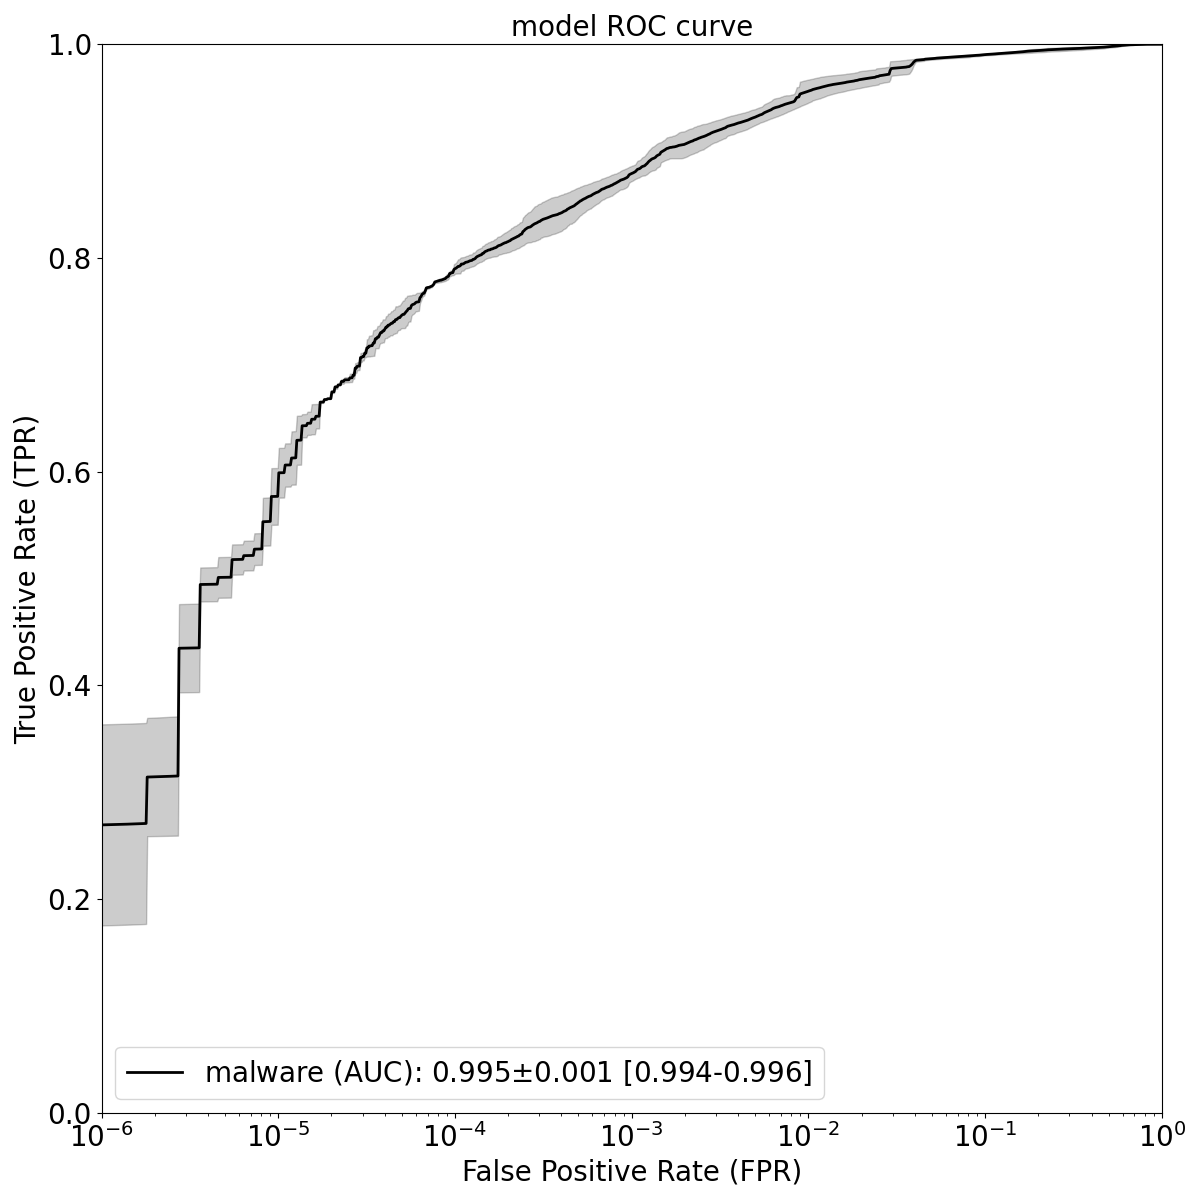
\includegraphics[width=0.78\textwidth]{./results/malware_roc_aloha.png}
        \vspace*{-1cm}
        \caption{ROC curve and AUC statistics of \textBF{ALOHA} model for the \textbf{Malware Label}. The line represents the \textit{mean} TPR at a given FPR, while the shaded region represents the \textit{standard deviation}. Statistics were computed over \textBF{3} training runs, each with random parameter initialization.}
        \label{fig:malwareRocAloha}
    \end{figure}
}

\newcommand{\malwareRocJointEmbedding}{
    \begin{figure}[H]
    	\vspace*{-0.7cm}
        \centering
        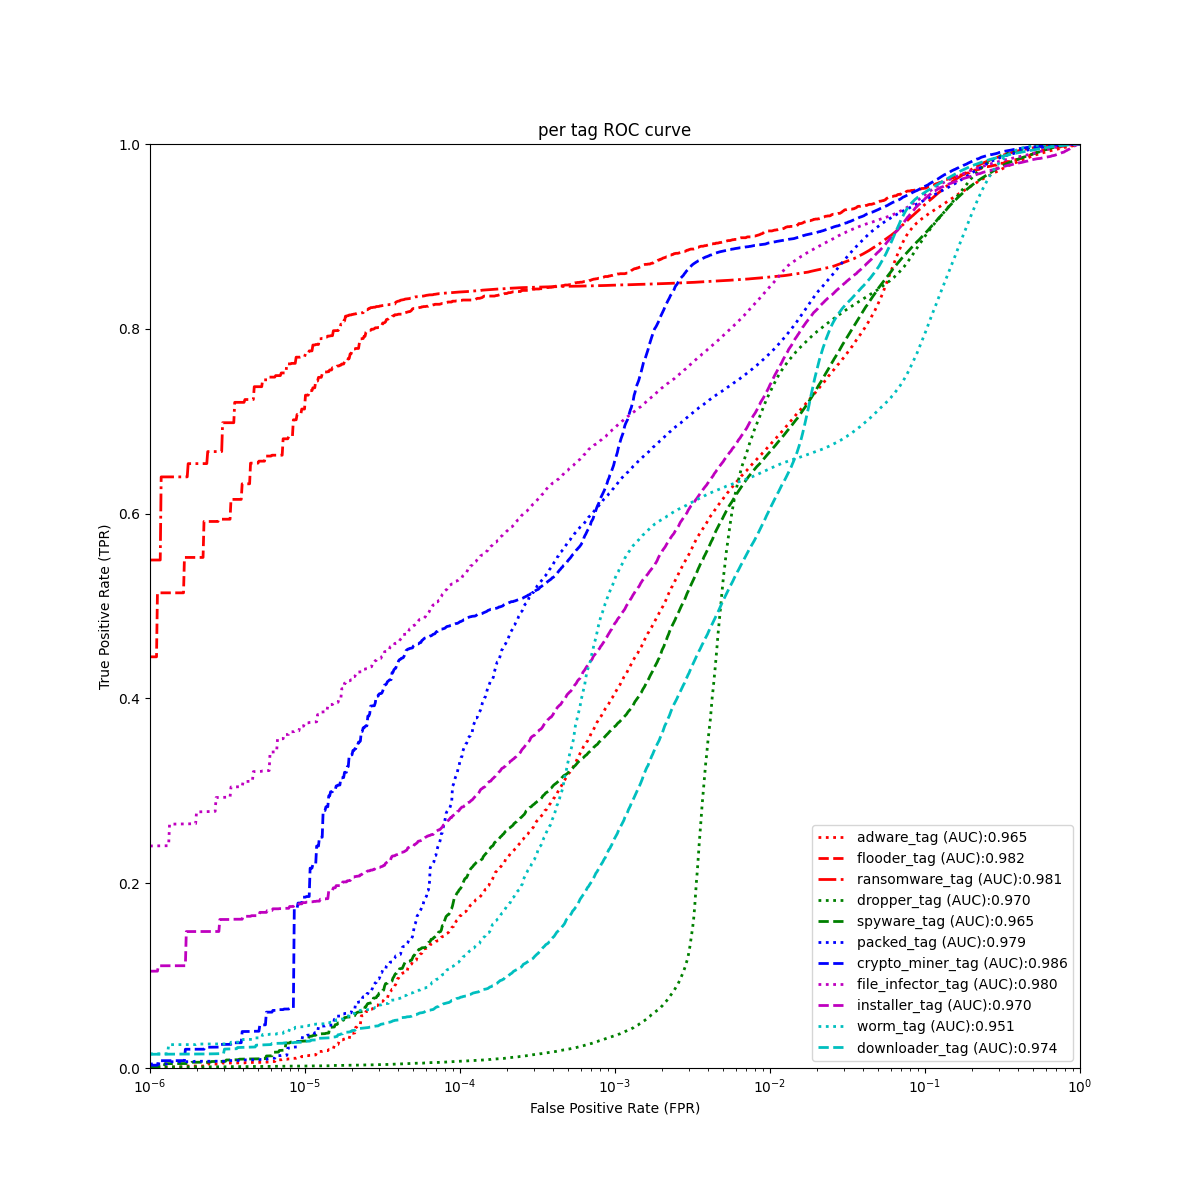
\includegraphics[width=0.78\textwidth]{./results/malware_roc_jointEmbedding.png}
        \vspace*{-1cm}
        \caption{ROC curve and AUC statistics of \textBF{Joint Embedding} model for the \textbf{Malware Label}. The line represents the \textit{mean} TPR at a given FPR, while the shaded region represents the \textit{standard deviation}. Statistics were computed over \textBF{3} training runs, each with random parameter initialization.}
        \label{fig:malwareRocJointEmbedding}
    \end{figure}
}

\newcommand{\malwareRocProposedMethod}{
    \begin{figure}[H]
    	\vspace*{-0.7cm}
        \centering
        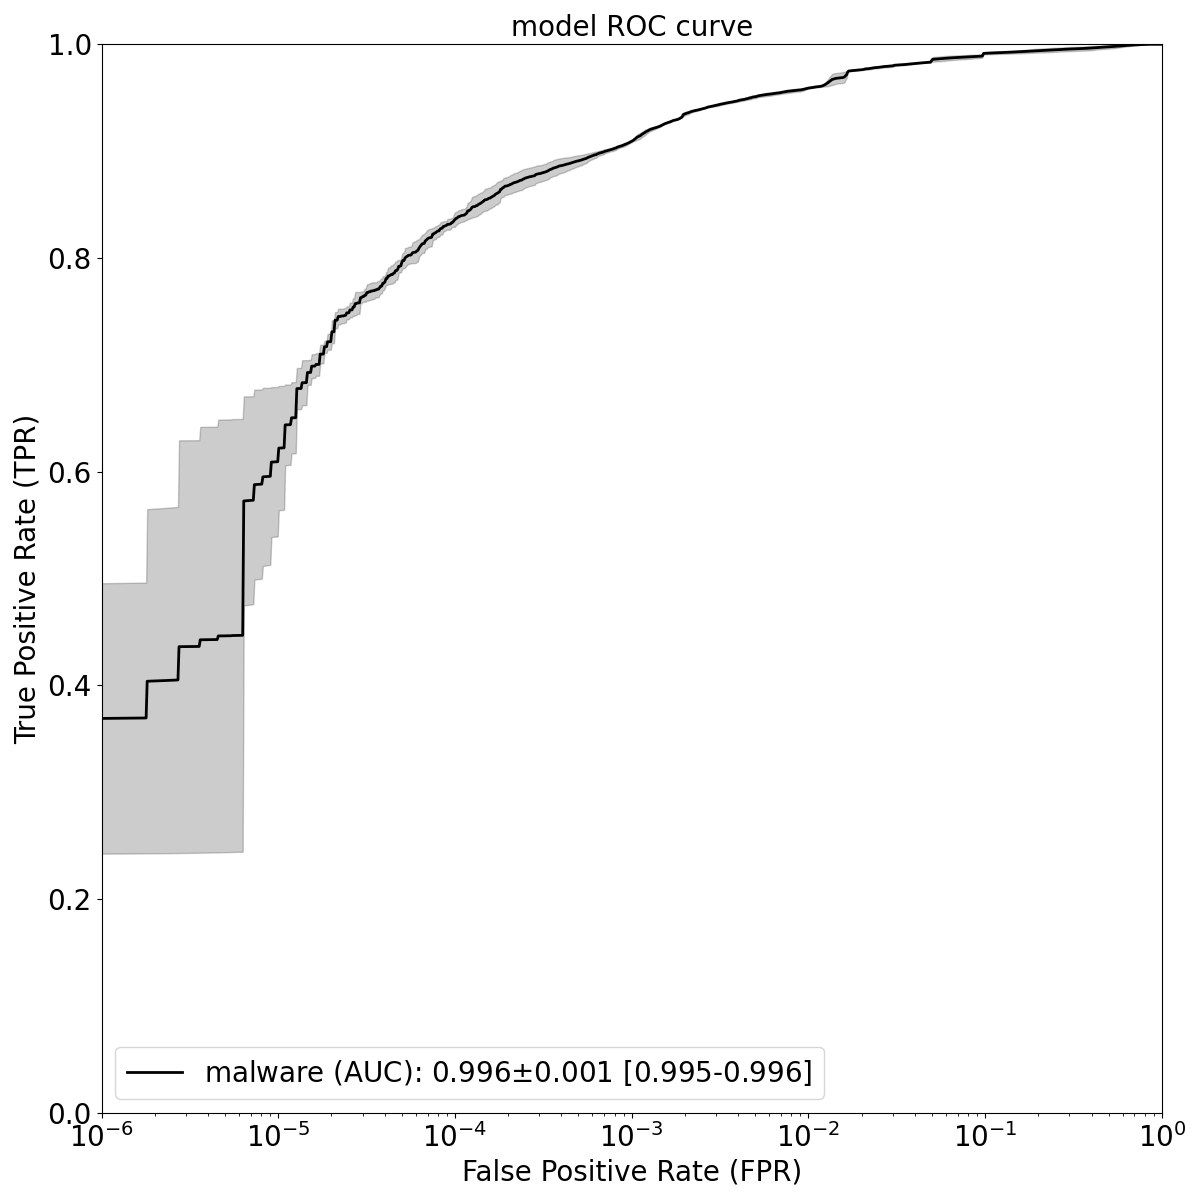
\includegraphics[width=0.78\textwidth]{./results/malware_roc_proposedModel.png}
        \vspace*{-1cm}
        \caption{ROC curve and AUC statistics of \textBF{Proposed Model} for the \textbf{Malware Label}. The line represents the \textit{mean} TPR at a given FPR, while the shaded region represents the \textit{standard deviation}. Statistics were computed over \textBF{3} training runs, each with random parameter initialization.}
        \label{fig:malwareRocProposedModel}
    \end{figure}
}

\newcommand{\tagResultsAucTable}{
    \begin{center}
        \begin{longtable}[c]{|P{2,8cm}||P{2,2cm} P{2,2cm} P{2,2cm} P{2,2cm}|}
            \hline
            AUC-ROC & ALOHA\newline (M/B only) & ALOHA & Joint\newline Embedding & Proposed\newline Model \\
            \hline
            \endfirsthead
            
            \caption*{\raggedright ...continued from previous page} \\
            \hline
            AUC-ROC & ALOHA\newline (M/B only) & ALOHA & Joint\newline Embedding & Proposed\newline Model \\
            \hline
            \endhead
            
            \caption*{\raggedleft ...continued on next page} \\
            \endfoot
            
            \caption{Mean and standard deviation AUC-ROC (Area Under Curve) of the different models for the the prediction of the different Tags. Results were aggregated over \textBF{3} training runs with different weight initializations and minibatch orderings. Best results are shown in \textbf{bold}.} \label{tab:tag_aucs}
            \endlastfoot
            
            Adware Tag & - & \textBF{0.973$\pm$0.000} & 0.971$\pm$0.002 & 0.972$\pm$0.002 \\
            Crypto-miner Tag & - & 0.985$\pm$0.002 & \textBF{0.990$\pm$0.001} & \textBF{0.990$\pm$0.001} \\
            Downloader Tag & - & 0.973$\pm$0.003 & \textBF{0.977$\pm$0.002} & 0.975$\pm$0.003 \\
            Dropper Tag & - & 0.972$\pm$0.001 & 0.973$\pm$0.001 & \textBF{0.976$\pm$0.001} \\
            File-infector Tag & - & 0.982$\pm$0.002 & 0.983$\pm$0.001 & \textBF{0.986$\pm$0.001} \\
            Flooder Tag & - & 0.985$\pm$0.001 & 0.985$\pm$0.000 & \textBF{0.988$\pm$0.001} \\
            Installer Tag & - & \textBF{0.976$\pm$0.001} & 0.974$\pm$0.000 & \textBF{0.976$\pm$0.001} \\
            Packed Tag & - & 0.978$\pm$0.001 & 0.978$\pm$0.003 & \textBF{0.983$\pm$0.002} \\
            Ransomware Tag & - & 0.979$\pm$0.003 & 0.979$\pm$0.004 & \textBF{0.984$\pm$0.005} \\
            Spyware Tag & - & 0.960$\pm$0.002 & 0.970$\pm$0.002 & \textBF{0.970$\pm$0.000} \\
            Worm Tag & - & \textBF{0.962$\pm$0.003} & 0.940$\pm$0.002 & 0.939$\pm$0.012 \\
            \hline
        \end{longtable}
    \end{center}
}

\newcommand{\tagResultsSummaryTable}{
    \begin{center}
        \begin{longtable}[c]{|P{3,2cm}||P{1,8cm} P{1,8cm} P{1,8cm} P{1,8cm} P{1,8cm}|}
            \hline
            & TPR & Accuracy & Precision & Recall & F1 score \\
            \hline
            \endfirsthead
            
            \caption*{\raggedright ...continued from previous page} \\
            \hline
            & TPR & Accuracy & Precision & Recall & F1 score \\
            \hline
            \endhead
            
            \caption*{\raggedleft ...continued on next page} \\
            \endfoot
            
            \caption{Summary of the mean and standard deviation results of the different models for the prediction of the different tags at \textbf{FPR} $=1\%$. Results were aggregated over \textBF{3} training runs with different weight initializations and minibatch orderings. Best results are shown in \textbf{bold}.} \label{tab:tag_results_summary}
            \endlastfoot
            
            \multicolumn{6}{|c|}{\textbf{Adware Tag} (at FPR $=1\%$)} \\
            \hline
            ALOHA (M/B only) & - & - & - & - & - \\
            ALOHA & \textBF{0.719$\pm$0.006} & \textBF{0.974$\pm$0.000} & \textBF{0.814$\pm$0.001} & \textBF{0.719$\pm$0.006} & \textBF{0.764$\pm$0.004} \\
            Joint Embedding & 0.696$\pm$0.016 & 0.973$\pm$0.001 & 0.809$\pm$0.003 & 0.696$\pm$0.016 & 0.748$\pm$0.010 \\
            Proposed Model & 0.684$\pm$0.013 & 0.972$\pm$0.001 & 0.807$\pm$0.003 & 0.684$\pm$0.013 & 0.741$\pm$0.009 \\
            \hline
            \multicolumn{6}{|c|}{\textbf{Crypto-miner Tag} (at FPR $=1\%$)} \\
            \hline
            ALOHA (M/B only) & - & - & - & - & - \\
            ALOHA & 0.879$\pm$0.000 & 0.988$\pm$0.000 & 0.552$\pm$0.000 & 0.879$\pm$0.000 & 0.678$\pm$0.000 \\
            Joint Embedding & 0.901$\pm$0.006 & \textBF{0.989$\pm$0.000} & 0.558$\pm$0.002 & 0.901$\pm$0.006 & 0.689$\pm$0.003 \\
            Proposed Model & \textBF{0.919$\pm$0.014} & \textBF{0.989$\pm$0.000} & \textBF{0.563$\pm$0.004} & \textBF{0.919$\pm$0.014} & \textBF{0.698$\pm$0.007} \\
            \hline
            \multicolumn{6}{|c|}{\textbf{Downloader Tag} (at FPR $=1\%$)} \\
            \hline
            ALOHA (M/B only) & - & - & - & - & - \\
            ALOHA & 0.619$\pm$0.020 & 0.959$\pm$0.002 & 0.850$\pm$0.004 & 0.619$\pm$0.020 & 0.716$\pm$0.014 \\
            Joint Embedding & \textBF{0.638$\pm$0.008} & \textBF{0.961$\pm$0.001} & \textBF{0.853$\pm$0.002} & \textBF{0.638$\pm$0.008} & \textBF{0.730$\pm$0.006} \\
            Proposed Model & 0.638$\pm$0.019 & 0.961$\pm$0.002 & 0.853$\pm$0.004 & 0.638$\pm$0.019 & 0.730$\pm$0.014 \\
            \hline
            \multicolumn{6}{|c|}{\textbf{Dropper Tag} (at FPR $=1\%$)} \\
            \hline
            ALOHA (M/B only) & - & - & - & - & - \\
            ALOHA & 0.672$\pm$0.026 & 0.949$\pm$0.003 & 0.908$\pm$0.003 & 0.672$\pm$0.026 & 0.772$\pm$0.019 \\
            Joint Embedding & \textBF{0.730$\pm$0.011} & \textBF{0.957$\pm$0.001} & \textBF{0.914$\pm$0.001} & \textBF{0.730$\pm$0.011} & \textBF{0.812$\pm$0.007} \\
            Proposed Model & 0.724$\pm$0.016 & 0.956$\pm$0.002 & 0.914$\pm$0.002 & 0.724$\pm$0.016 & 0.808$\pm$0.011 \\
            \hline
            \multicolumn{6}{|c|}{\textbf{File-infector Tag} (at FPR $=1\%$)} \\
            \hline
            ALOHA (M/B only) & - & - & - & - & - \\
            ALOHA & 0.851$\pm$0.008 & 0.968$\pm$0.001 & 0.943$\pm$0.000 & 0.851$\pm$0.008 & 0.894$\pm$0.004 \\
            Joint Embedding & 0.857$\pm$0.009 & 0.969$\pm$0.001 & 0.943$\pm$0.001 & 0.857$\pm$0.009 & 0.898$\pm$0.005 \\
            Proposed Model & \textBF{0.872$\pm$0.011} & \textBF{0.971$\pm$0.002} & \textBF{0.944$\pm$0.001} & \textBF{0.872$\pm$0.011} & \textBF{0.907$\pm$0.006} \\
            \hline
            \multicolumn{6}{|c|}{\textbf{Flooder Tag} (at FPR $=1\%$)} \\
            \hline
            ALOHA (M/B only) & - & - & - & - & - \\
            ALOHA & 0.897$\pm$0.013 & \textBF{0.990$\pm$0.000} & 0.140$\pm$0.002 & 0.897$\pm$0.013 & 0.242$\pm$0.003 \\
            Joint Embedding & 0.910$\pm$0.006 & \textBF{0.990$\pm$0.000} & 0.141$\pm$0.001 & 0.910$\pm$0.006 & \textBF{0.245$\pm$0.001} \\
            Proposed Model & \textBF{0.913$\pm$0.005} & \textBF{0.990$\pm$0.000} & \textBF{0.142$\pm$0.001} & \textBF{0.913$\pm$0.005} & \textBF{0.245$\pm$0.001} \\
            \hline
            \multicolumn{6}{|c|}{\textbf{Installer Tag} (at FPR $=1\%$)} \\
            \hline
            ALOHA (M/B only) & - & - & - & - & - \\
            ALOHA & 0.755$\pm$0.009 & \textBF{0.986$\pm$0.000} & \textBF{0.578$\pm$0.003} & 0.755$\pm$0.009 & 0.655$\pm$0.005 \\
            Joint Embedding & 0.752$\pm$0.021 & \textBF{0.986$\pm$0.000} & 0.576$\pm$0.007 & 0.752$\pm$0.021 & 0.653$\pm$0.012 \\
            Proposed Model & \textBF{0.759$\pm$0.052} & 0.986$\pm$0.001 & 0.578$\pm$0.017 & \textBF{0.759$\pm$0.052} & \textBF{0.656$\pm$0.030} \\
            \hline
            \multicolumn{6}{|c|}{\textbf{Packed Tag} (at FPR $=1\%$)} \\
            \hline
            ALOHA (M/B only) & - & - & - & - & - \\
            ALOHA & 0.675$\pm$0.017 & 0.947$\pm$0.002 & 0.914$\pm$0.002 & 0.675$\pm$0.017 & 0.776$\pm$0.012 \\
            Joint Embedding & 0.731$\pm$0.019 & 0.955$\pm$0.003 & 0.920$\pm$0.002 & 0.731$\pm$0.019 & 0.815$\pm$0.012 \\
            Proposed Model & \textBF{0.758$\pm$0.016} & \textBF{0.958$\pm$0.002} & \textBF{0.923$\pm$0.002} & \textBF{0.758$\pm$0.016} & \textBF{0.832$\pm$0.010} \\
            \hline
            \multicolumn{6}{|c|}{\textbf{Ransomware Tag} (at FPR $=1\%$)} \\
            \hline
            ALOHA (M/B only) & - & - & - & - & - \\
            ALOHA & 0.849$\pm$0.001 & \textBF{0.983$\pm$0.000} & 0.824$\pm$0.000 & 0.849$\pm$0.001 & 0.836$\pm$0.001 \\
            Joint Embedding & 0.855$\pm$0.002 & \textBF{0.983$\pm$0.000} & 0.825$\pm$0.000 & 0.855$\pm$0.002 & 0.840$\pm$0.001 \\
            Proposed Model & \textBF{0.858$\pm$0.003} & \textBF{0.983$\pm$0.000} & \textBF{0.826$\pm$0.001} & \textBF{0.858$\pm$0.003} & \textBF{0.841$\pm$0.002} \\
            \hline
            \multicolumn{6}{|c|}{\textbf{Spyware Tag} (at FPR $=1\%$)} \\
            \hline
            ALOHA (M/B only) & - & - & - & - & - \\
            ALOHA & 0.604$\pm$0.007 & 0.949$\pm$0.001 & 0.878$\pm$0.001 & 0.604$\pm$0.007 & 0.716$\pm$0.005 \\
            Joint Embedding & \textBF{0.662$\pm$0.017} & \textBF{0.955$\pm$0.002} & \textBF{0.888$\pm$0.003} & \textBF{0.662$\pm$0.017} & \textBF{0.759$\pm$0.012} \\
            Proposed Model & 0.651$\pm$0.007 & 0.954$\pm$0.001 & 0.886$\pm$0.001 & 0.651$\pm$0.007 & 0.751$\pm$0.005 \\
            \hline
            \multicolumn{6}{|c|}{\textbf{Worm Tag} (at FPR $=1\%$)} \\
            \hline
            ALOHA (M/B only) & - & - & - & - & - \\
            ALOHA & \textBF{0.652$\pm$0.014} & \textBF{0.936$\pm$0.002} & \textBF{0.925$\pm$0.002} & \textBF{0.652$\pm$0.014} & \textBF{0.764$\pm$0.010} \\
            Joint Embedding & 0.647$\pm$0.017 & 0.936$\pm$0.003 & 0.924$\pm$0.002 & 0.647$\pm$0.017 & 0.761$\pm$0.013 \\
            Proposed Model & 0.641$\pm$0.021 & 0.935$\pm$0.003 & 0.923$\pm$0.002 & 0.641$\pm$0.021 & 0.757$\pm$0.016 \\
            \hline
        \end{longtable}
    \end{center}
}
%\newcommand{\adwareTagResultsAucTable}{
    \begin{table}[H]
        \centering
        \begin{tabular}{|p{2,8cm}||P{2,4cm} P{2,4cm} P{2,4cm}|}
            \hline
            Adware Tag & ALOHA\newline (M/B only) & ALOHA & Proposed\newline Model \\
            \hline
            AUC-ROC & - & 0.618$\pm$0.017 & 0.544$\pm$0.056 \\
            \hline
        \end{tabular}
        \caption[Adware Tag prediction task AUC-ROC results]{AUC-ROC (Area Under Curve) of the different models for the \textbf{Adware Tag} prediction task. Results were aggregated over \textBF{2} training runs with different weight initializations and minibatch orderings. Best results are shown in \textbf{bold}.} \label{tab:adwareTag_auc}
    \end{table}
}

\newcommand{\adwareTagResultsAtFprTable}{
    \begin{center}
        \begin{longtable}[c]{|P{3,2cm}||P{1,8cm} P{1,8cm} P{1,8cm} P{1,8cm} P{1,8cm}|}
            \hline
            Adware Tag & \multicolumn{5}{c|}{{FPR}} \\
            & $10^{-5}$ & $10^{-4}$ & $10^{-3}$ & $10^{-2}$ & $10^{-1}$ \\
            \hline
            \endfirsthead

            \caption*{\raggedright ...continued from previous page} \\
            \hline
            Adware Tag & \multicolumn{5}{c|}{\textbf{FPR}} \\
            & $10^{-5}$ & $10^{-4}$ & $10^{-3}$ & $10^{-2}$ & $10^{-1}$ \\
            \hline
            \endhead

            \caption*{\raggedleft ...continued on next page} \\
            \endfoot

            \caption[Adware Tag prediction task results]{Mean and standard deviation results (TPR, Accuracy, Recall, Precision and F1-Score) of the different models for the \textbf{Adware Tag} prediction task at different \textbf{FPR}s (\textit{False Positive Rates}). Results were aggregated over \textBF{2} training runs with different weight initializations and minibatch orderings. Best results are shown in \textbf{bold}. Under \textbf{TPR} results are also presented the percentage reduction in mean detection error and in ROC curve standard deviation introduced by the \textit{Proposed Model} with respect to both \textit{ALOHA} model and \textit{Joint Embedding}.} \label{tab:adwareTag_results_at_fpr} \\
            \endlastfoot

            \multicolumn{6}{|c|}{\textbf{TPR}} \\
            \hline
            ALOHA (M/B only) & - & - & - & - & - \\
            ALOHA & \textBF{0.002$\pm$0.002} & \textBF{0.002$\pm$0.002} & \textBF{0.002$\pm$0.002} & \textBF{0.011$\pm$0.011} & 0.068$\pm$0.014 \\
            Proposed Model & 0.000$\pm$0.000 & 0.000$\pm$0.000 & 0.000$\pm$0.000 & 0.005$\pm$0.005 & 0.043$\pm$0.039 \\
            \hline
            Error Reduction wrt\newline ALOHA (M/B only) & - & - & - & - & - \\
            Error Reduction wrt\newline ALOHA & -0.2\% & -0.2\% & -0.2\% & -0.6\% & -2.7\% \\
            \hline
            Std Reduction wrt\newline ALOHA (M/B only) & - & - & - & - & - \\
            Std Reduction wrt\newline ALOHA & 100.0\% & 100.0\% & 100.0\% & 54.5\% & -178.6\% \\
            \hline
            \multicolumn{6}{|c|}{\textbf{Accuracy}} \\
            \hline
            ALOHA (M/B only) & - & - & - & - & - \\
            ALOHA & \textBF{0.910$\pm$0.000} & \textBF{0.910$\pm$0.000} & \textBF{0.910$\pm$0.000} & 0.904$\pm$0.005 & 0.825$\pm$0.001 \\
            Proposed Model & \textBF{0.910$\pm$0.000} & \textBF{0.910$\pm$0.000} & 0.908$\pm$0.001 & 0.903$\pm$0.000 & 0.823$\pm$0.004 \\
            \hline
            \multicolumn{6}{|c|}{\textbf{Recall}} \\
            \hline
            ALOHA (M/B only) & - & - & - & - & - \\
            ALOHA & \textBF{0.002$\pm$0.002} & \textBF{0.002$\pm$0.002} & \textBF{0.002$\pm$0.002} & \textBF{0.011$\pm$0.011} & 0.068$\pm$0.014 \\
            Proposed Model & 0.000$\pm$0.000 & 0.000$\pm$0.000 & 0.000$\pm$0.000 & 0.005$\pm$0.005 & 0.043$\pm$0.039 \\
            \hline
            \multicolumn{6}{|c|}{\textbf{Precision}} \\
            \hline
            ALOHA (M/B only) & - & - & - & - & - \\
            ALOHA & \textBF{1.000$\pm$0.000} & \textBF{1.000$\pm$0.000} & \textBF{0.167$\pm$0.167} & \textBF{0.066$\pm$0.066} & 0.063$\pm$0.012 \\
            Proposed Model & \textBF{1.000$\pm$0.000} & \textBF{1.000$\pm$0.000} & 0.000$\pm$0.000 & 0.045$\pm$0.045 & 0.040$\pm$0.035 \\
            \hline
            \multicolumn{6}{|c|}{\textbf{F1 Score}} \\
            \hline
            ALOHA (M/B only) & - & - & - & - & - \\
            ALOHA & \textBF{0.005$\pm$0.005} & \textBF{0.005$\pm$0.005} & \textBF{0.004$\pm$0.004} & \textBF{0.019$\pm$0.019} & 0.065$\pm$0.013 \\
            Proposed Model & 0.000$\pm$0.000 & 0.000$\pm$0.000 & 0.000$\pm$0.000 & 0.008$\pm$0.008 & 0.041$\pm$0.037 \\
            \hline
        \end{longtable}
    \end{center}
}

\newcommand{\adwareTagResultsSummaryTable}{
    \begin{table}[H]
        \centering
        \begin{tabular}{|P{3,2cm}||P{1,8cm} P{1,8cm} P{1,8cm} P{1,8cm} P{1,8cm}|}
            \hline
            \multicolumn{6}{|c|}{Adware Tag (at FPR $=1\%$)} \\
            \hline
            Model & TPR & Accuracy & Precision & Recall & F1 score \\
            \hline
            ALOHA (M/B only) & - & - & - & - & - \\
            ALOHA & \textBF{0.011$\pm$0.011} & 0.904$\pm$0.005 & \textBF{0.066$\pm$0.066} & \textBF{0.011$\pm$0.011} & \textBF{0.019$\pm$0.019} \\
            Proposed Model & 0.005$\pm$0.005 & 0.903$\pm$0.000 & 0.045$\pm$0.045 & 0.005$\pm$0.005 & 0.008$\pm$0.008 \\
            \hline
        \end{tabular}
        \caption[Summary of Adware Tag prediction task results]{Summary of the mean and standard deviation results of the different models for the \textbf{Adware Tag} prediction task at \textbf{FPR} $=1\%$. Results were aggregated over \textBF{2} training runs with different weight initializations and minibatch orderings. Best results are shown in \textbf{bold}.} \label{tab:adwareTag_result_summary}
    \end{table}
}

\newcommand{\adwareTagRocAlohaMB}{
    \begin{figure}[H]
        \vspace*{-0.5cm}
        \centering
        \includegraphics[width=0.6\textwidth]{./results/adware_tag_roc_alohaMB.png}
        \vspace*{-0.2cm}
        \caption[Adware Tag prediction task ALOHA (M/B only) ROC curve]{ROC curve and AUC statistics of \textBF{ALOHA (M/B only)} model for the \textbf{Adware Tag}. The line represents the \textit{mean} TPR at a given FPR, while the shaded region represents the \textit{standard deviation}. Statistics were computed over \textBF{2} training runs, each with random parameter initialization.}
        \label{fig:adwareTagRocAlohaMB}
    \end{figure}
}

\newcommand{\adwareTagRocAloha}{
    \begin{figure}[H]
        \vspace*{-0.5cm}
        \centering
        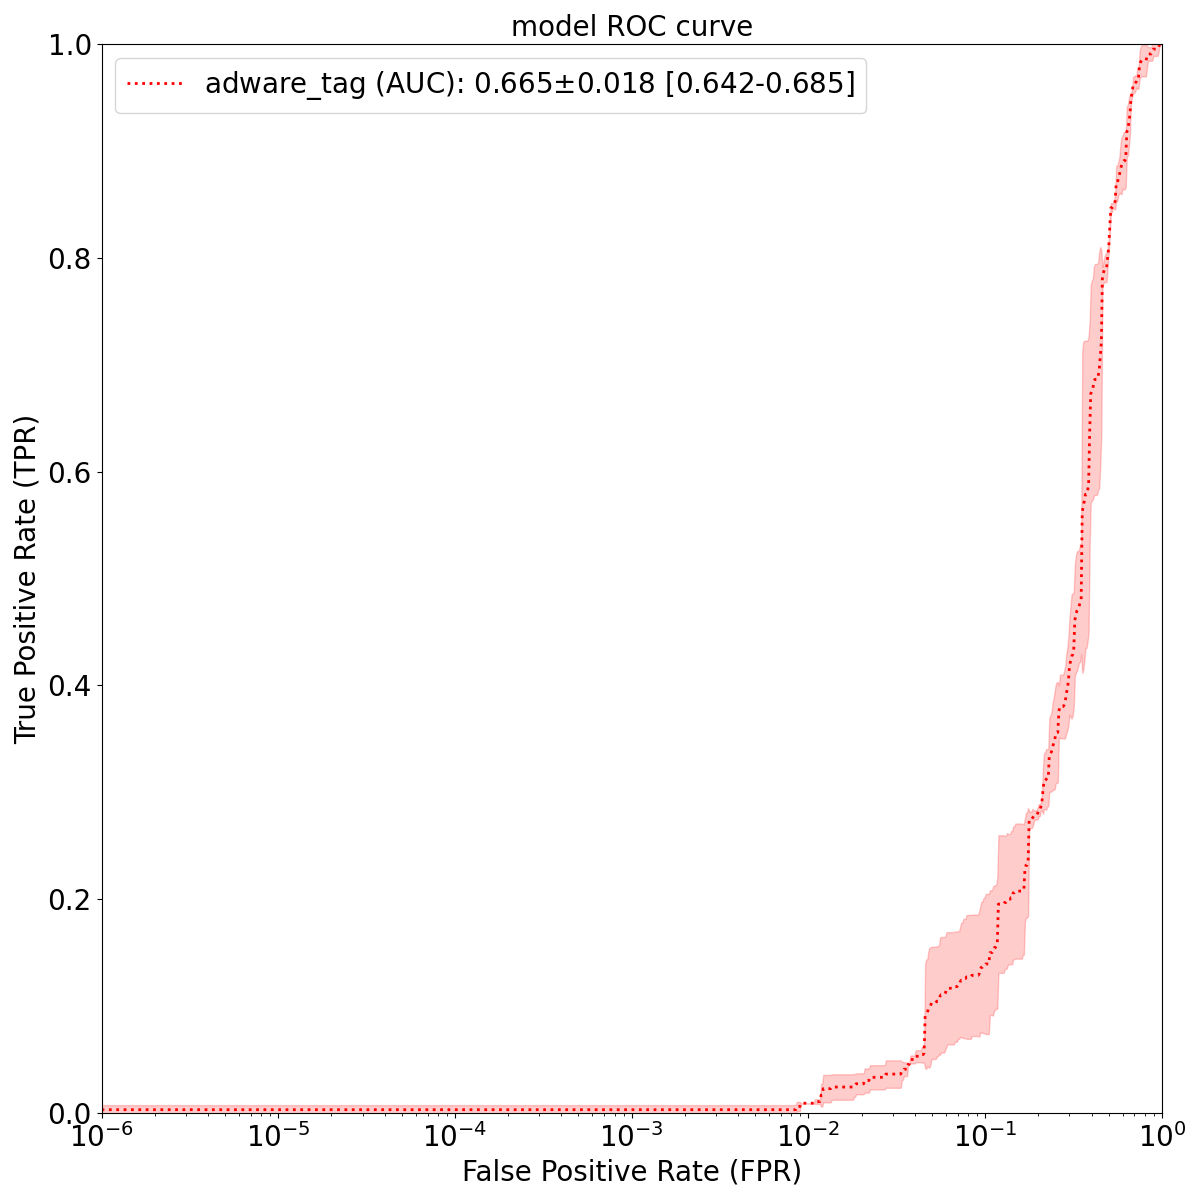
\includegraphics[width=0.6\textwidth]{./results/adware_tag_roc_aloha.png}
        \vspace*{-0.2cm}
        \caption[Adware Tag prediction task ALOHA ROC curve]{ROC curve and AUC statistics of \textBF{ALOHA} model for the \textbf{Adware Tag}. The line represents the \textit{mean} TPR at a given FPR, while the shaded region represents the \textit{standard deviation}. Statistics were computed over \textBF{2} training runs, each with random parameter initialization.}
        \label{fig:adwareTagRocAloha}
    \end{figure}
}

\newcommand{\adwareTagRocProposedMethod}{
    \begin{figure}[H]
        \vspace*{-0.5cm}
        \centering
        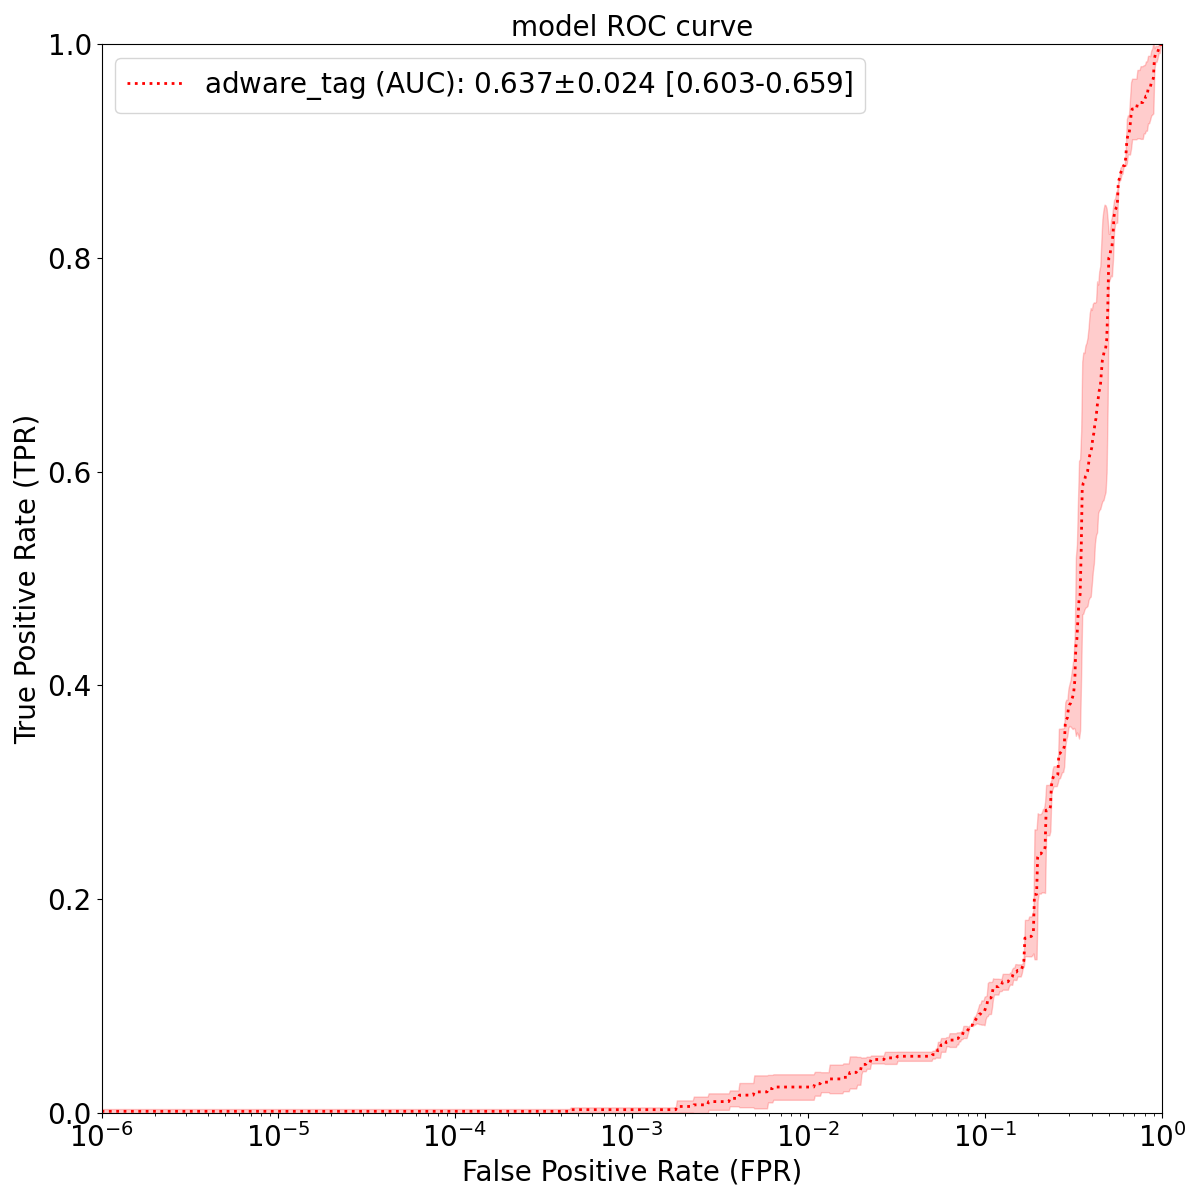
\includegraphics[width=0.6\textwidth]{./results/adware_tag_roc_proposedModel.png}
        \vspace*{-0.2cm}
        \caption[Adware Tag prediction task Proposed Model ROC curve]{ROC curve and AUC statistics of \textBF{Proposed Model} for the \textbf{Adware Tag}. The line represents the \textit{mean} TPR at a given FPR, while the shaded region represents the \textit{standard deviation}. Statistics were computed over \textBF{2} training runs, each with random parameter initialization.}
        \label{fig:adwareTagRocProposedModel}
    \end{figure}
}

%\newcommand{\cryptoMinerTagResultsAucTable}{
    \begin{table}[H]
        \centering
        \begin{tabular}{|p{2,8cm}||p{2,8cm} p{2,8cm} p{2,8cm}|}
            \hline
            Crypto-miner Tag & ALOHA & Joint Embedding & Proposed Model \\
            \hline
            AUC-ROC & \textBF{0.639$\pm$0.039} & 0.496$\pm$0.020 & 0.468$\pm$0.025 \\
            \hline
        \end{tabular}
        \caption{AUC-ROC (Area Under Curve) of the different models for the \textbf{Crypto-miner Tag} prediction task. Results were aggregated over \textBF{3} training runs with different weight initializations and minibatch orderings. Best results are shown in \textbf{bold}.} \label{tab:cryptoMinerTag_auc}
    \end{table}
}

\newcommand{\cryptoMinerTagResultsAtFprTable}{
    \begin{center}
        \begin{longtable}[c]{|p{3,2cm}||p{1,8cm} p{1,8cm} p{1,8cm} p{1,8cm} p{1,8cm}|}
            \hline
            Crypto-miner Tag & \multicolumn{5}{c|}{{FPR}} \\
            & $10^{-5}$ & $10^{-4}$ & $10^{-3}$ & $10^{-2}$ & $10^{-1}$ \\
            \hline
            \endfirsthead

            \caption*{\raggedright ...continued from previous page} \\
            \hline
            Crypto-miner Tag & \multicolumn{5}{c|}{\textbf{FPR}} \\
            & $10^{-5}$ & $10^{-4}$ & $10^{-3}$ & $10^{-2}$ & $10^{-1}$ \\
            \hline
            \endhead

            \caption*{\raggedleft ...continued on next page} \\
            \endfoot

            \caption{Mean and standard deviation results (TPR, Accuracy, Recall, Precision and F1-Score) of the different models for the \textbf{Crypto-miner Tag} prediction task at different \textbf{FPR}s (\textit{False Positive Rates}). Results were aggregated over \textBF{3} training runs with different weight initializations and minibatch orderings. Best results are shown in \textbf{bold}. Under \textbf{TPR} results are also presented the percentage reduction in mean detection error and in ROC curve standard deviation introduced by the \textit{Proposed Model} with respect to both \textit{ALOHA} model and \textit{Joint Embedding}.} \label{tab:cryptoMinerTag_results_at_fpr} \\
            \endlastfoot

            \multicolumn{6}{|c|}{\textbf{TPR}} \\
            \hline
            ALOHA & 0.000$\pm$0.000 & 0.000$\pm$0.000 & 0.000$\pm$0.000 & 0.027$\pm$0.000 & \textBF{0.198$\pm$0.025} \\
            Joint Embedding & \textBF{0.009$\pm$0.013} & \textBF{0.009$\pm$0.013} & \textBF{0.009$\pm$0.013} & \textBF{0.036$\pm$0.051} & 0.144$\pm$0.034 \\
            Proposed Model & 0.000$\pm$0.000 & 0.000$\pm$0.000 & 0.000$\pm$0.000 & 0.009$\pm$0.013 & 0.072$\pm$0.034 \\
            \hline
            Error Reduction wrt \newline ALOHA & 0.0\% & 0.0\% & 0.0\% & -1.8\% & -15.7\% \\
            Error Reduction wrt \newline Joint Embedding & -0.9\% & -0.9\% & -0.9\% & -2.8\% & -8.4\% \\
            \hline
            Std Reduction wrt \newline ALOHA & 0.0\% & 0.0\% & 0.0\% & 0.0\% & -36.0\% \\
            Std Reduction wrt \newline Joint Embedding & 100.0\% & 100.0\% & 100.0\% & 74.5\% & 0.0\% \\
            \hline
            \multicolumn{6}{|c|}{\textbf{Accuracy}} \\
            \hline
            ALOHA & \textBF{0.985$\pm$0.000} & \textBF{0.985$\pm$0.000} & 0.984$\pm$0.000 & 0.977$\pm$0.001 & 0.892$\pm$0.001 \\
            Joint Embedding & \textBF{0.985$\pm$0.000} & \textBF{0.985$\pm$0.000} & \textBF{0.985$\pm$0.000} & 0.982$\pm$0.002 & 0.891$\pm$0.003 \\
            Proposed Model & \textBF{0.985$\pm$0.000} & \textBF{0.985$\pm$0.000} & 0.984$\pm$0.000 & \textBF{0.983$\pm$0.002} & \textBF{0.894$\pm$0.009} \\
            \hline
            \multicolumn{6}{|c|}{\textbf{Recall}} \\
            \hline
            ALOHA & 0.000$\pm$0.000 & 0.000$\pm$0.000 & 0.000$\pm$0.000 & 0.027$\pm$0.000 & \textBF{0.198$\pm$0.025} \\
            Joint Embedding & \textBF{0.009$\pm$0.013} & \textBF{0.009$\pm$0.013} & \textBF{0.009$\pm$0.013} & \textBF{0.036$\pm$0.051} & 0.144$\pm$0.034 \\
            Proposed Model & 0.000$\pm$0.000 & 0.000$\pm$0.000 & 0.000$\pm$0.000 & 0.009$\pm$0.013 & 0.072$\pm$0.034 \\
            \hline
            \multicolumn{6}{|c|}{\textbf{Precision}} \\
            \hline
            ALOHA & \textBF{1.000$\pm$0.000} & \textBF{1.000$\pm$0.000} & 0.000$\pm$0.000 & 0.048$\pm$0.008 & \textBF{0.030$\pm$0.004} \\
            Joint Embedding & \textBF{1.000$\pm$0.000} & \textBF{1.000$\pm$0.000} & \textBF{0.333$\pm$0.471} & \textBF{0.067$\pm$0.094} & 0.022$\pm$0.006 \\
            Proposed Model & \textBF{1.000$\pm$0.000} & \textBF{1.000$\pm$0.000} & 0.000$\pm$0.000 & 0.022$\pm$0.031 & 0.011$\pm$0.005 \\
            \hline
            \multicolumn{6}{|c|}{\textbf{F1 Score}} \\
            \hline
            ALOHA & 0.000$\pm$0.000 & 0.000$\pm$0.000 & 0.000$\pm$0.000 & 0.034$\pm$0.002 & \textBF{0.052$\pm$0.007} \\
            Joint Embedding & \textBF{0.018$\pm$0.025} & \textBF{0.018$\pm$0.025} & \textBF{0.018$\pm$0.025} & \textBF{0.047$\pm$0.066} & 0.039$\pm$0.010 \\
            Proposed Model & 0.000$\pm$0.000 & 0.000$\pm$0.000 & 0.000$\pm$0.000 & 0.013$\pm$0.018 & 0.019$\pm$0.008 \\
            \hline
        \end{longtable}
    \end{center}
}

\newcommand{\cryptoMinerTagResultsSummaryTable}{
    \begin{table}[H]
        \centering
        \begin{tabular}{|p{3,2cm}||p{1,8cm} p{1,8cm} p{1,8cm} p{1,8cm} p{1,8cm}|}
            \hline
            \multicolumn{6}{|c|}{Crypto-miner Tag (at FPR $=1\%$)} \\
            \hline
            Model & TPR & Accuracy & Precision & Recall & F1 score \\
            \hline
            ALOHA & 0.027$\pm$0.000 & 0.977$\pm$0.001 & 0.048$\pm$0.008 & 0.027$\pm$0.000 & 0.034$\pm$0.002 \\
            Joint Embedding & \textBF{0.036$\pm$0.051} & 0.982$\pm$0.002 & \textBF{0.067$\pm$0.094} & \textBF{0.036$\pm$0.051} & \textBF{0.047$\pm$0.066} \\
            Proposed Model & 0.009$\pm$0.013 & \textBF{0.983$\pm$0.002} & 0.022$\pm$0.031 & 0.009$\pm$0.013 & 0.013$\pm$0.018 \\
            \hline
        \end{tabular}
        \caption{Summary of the mean and standard deviation results of the different models for the \textbf{Crypto-miner Tag} prediction task at \textbf{FPR} $=1\%$. Results were aggregated over \textBF{3} training runs with different weight initializations and minibatch orderings. Best results are shown in \textbf{bold}.} \label{tab:cryptoMinerTag_result_summary}
    \end{table}
}

\newcommand{\cryptoMinerTagRocAloha}{
    \begin{figure}[H]
        \vspace*{-0.5cm}
        \centering
        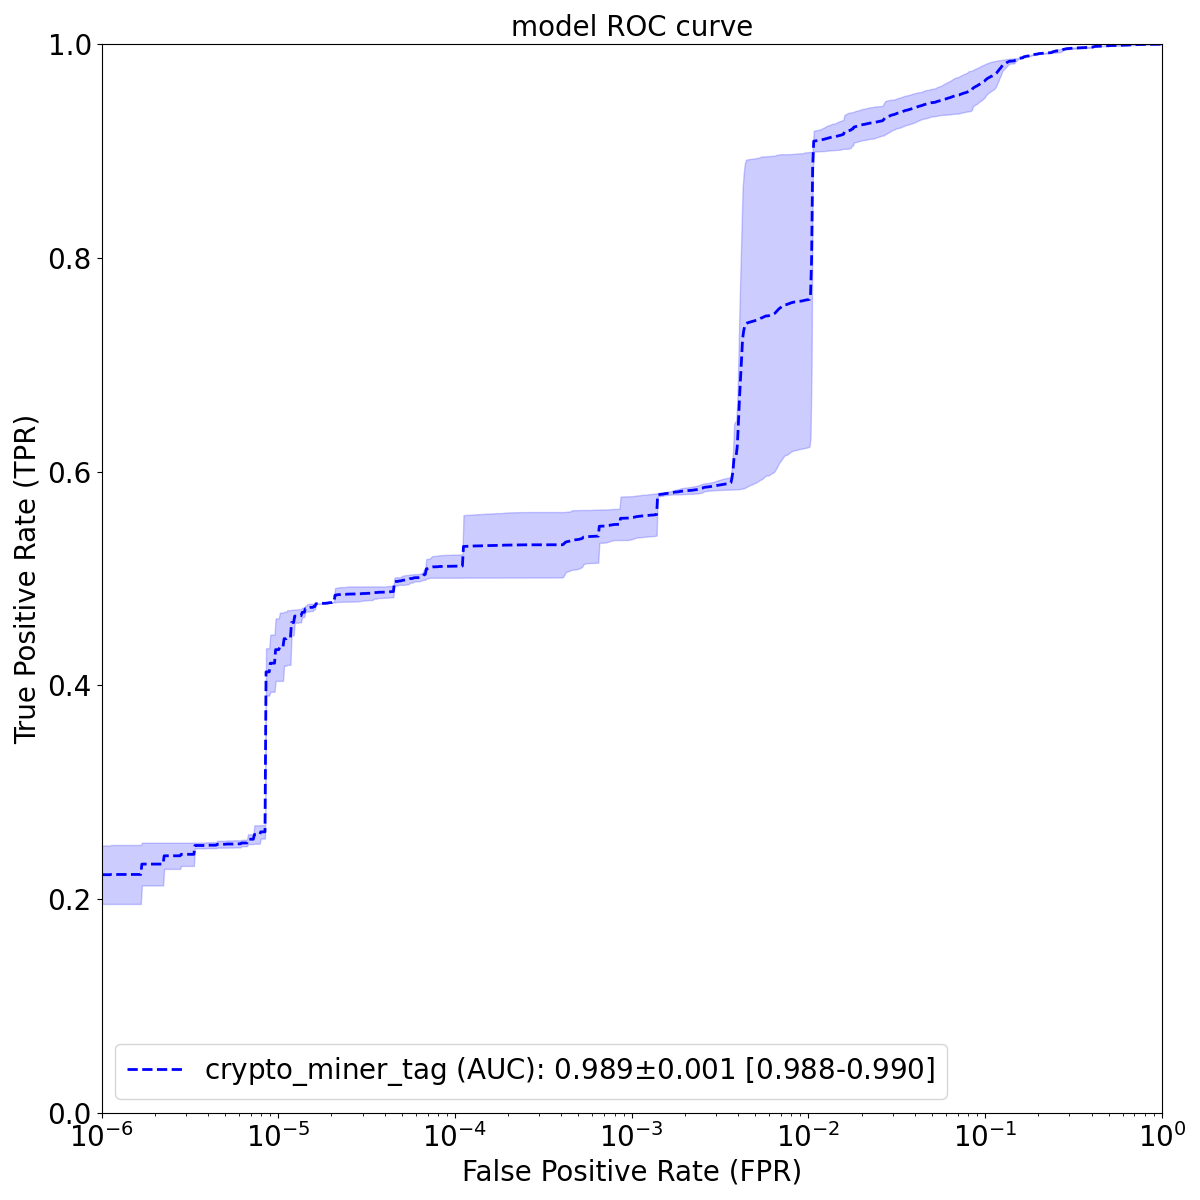
\includegraphics[width=0.6\textwidth]{./results/crypto_miner_tag_roc_aloha.png}
        \vspace*{-0.2cm}
        \caption{ROC curve and AUC statistics of \textBF{ALOHA} model for the \textbf{Crypto-miner Tag}. The line represents the \textit{mean} TPR at a given FPR, while the shaded region represents the \textit{standard deviation}. Statistics were computed over \textBF{3} training runs, each with random parameter initialization.}
        \label{fig:cryptoMinerTagRocAloha}
    \end{figure}
}

\newcommand{\cryptoMinerTagRocJointEmbedding}{
    \begin{figure}[H]
        \vspace*{-0.5cm}
        \centering
        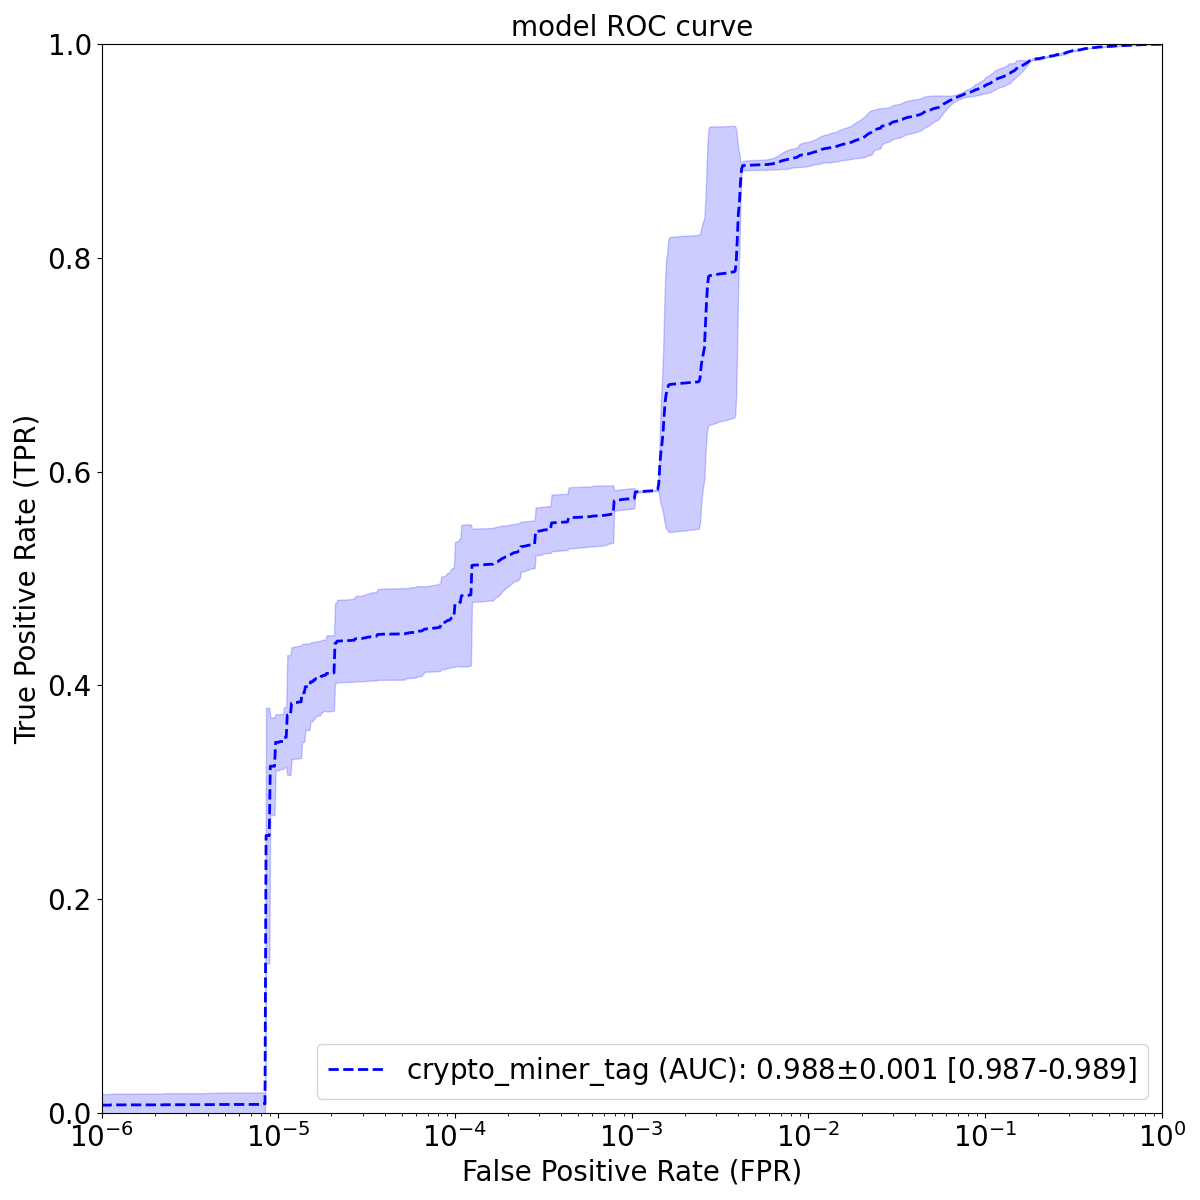
\includegraphics[width=0.6\textwidth]{./results/crypto_miner_tag_roc_jointEmbedding.png}
        \vspace*{-0.2cm}
        \caption{ROC curve and AUC statistics of \textBF{Joint Embedding} model for the \textbf{Crypto-miner Tag}. The line represents the \textit{mean} TPR at a given FPR, while the shaded region represents the \textit{standard deviation}. Statistics were computed over \textBF{3} training runs, each with random parameter initialization.}
        \label{fig:cryptoMinerTagRocJointEmbedding}
    \end{figure}
}

\newcommand{\cryptoMinerTagRocProposedMethod}{
    \begin{figure}[H]
        \vspace*{-0.5cm}
        \centering
        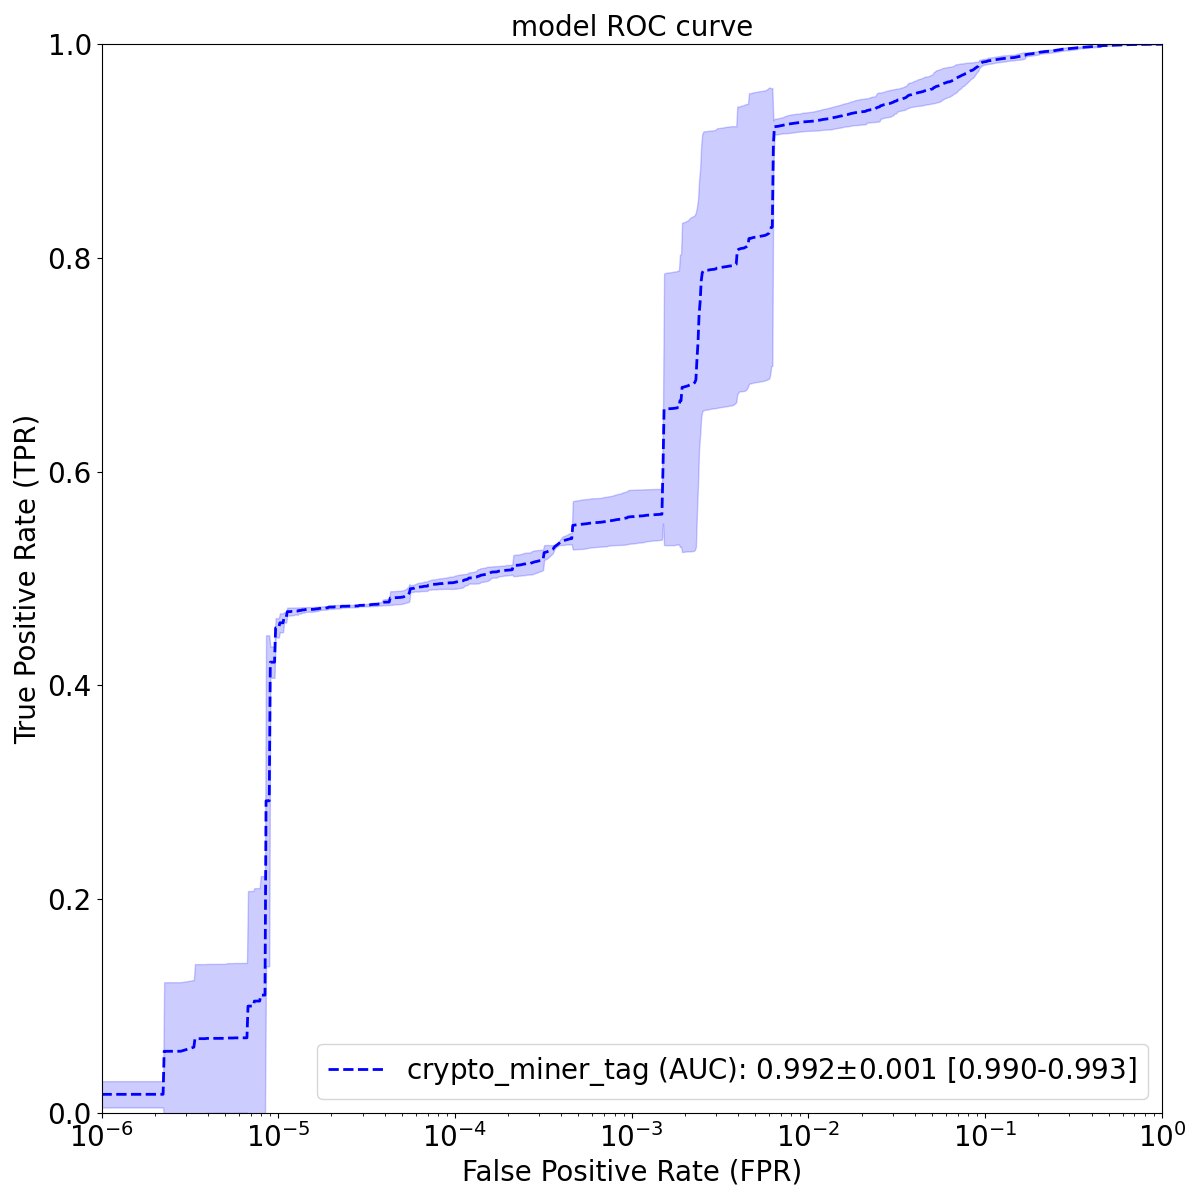
\includegraphics[width=0.6\textwidth]{./results/crypto_miner_tag_roc_proposedModel.png}
        \vspace*{-0.2cm}
        \caption{ROC curve and AUC statistics of \textBF{Proposed Model} for the \textbf{Crypto-miner Tag}. The line represents the \textit{mean} TPR at a given FPR, while the shaded region represents the \textit{standard deviation}. Statistics were computed over \textBF{3} training runs, each with random parameter initialization.}
        \label{fig:cryptoMinerTagRocProposedModel}
    \end{figure}
}

%\newcommand{\downloaderTagResultsAucTable}{
    \begin{table}[h!]
        \centering
        \begin{tabular}{|p{2,8cm}||P{2,2cm} P{2,2cm} P{2,2cm} P{2,2cm}|}
            \hline
            Downloader Tag & ALOHA\newline (M/B only) & ALOHA & Joint\newline Embedding & Proposed\newline Model \\
            \hline
            AUC-ROC & - & 0.973$\pm$0.003 & \textBF{0.977$\pm$0.002} & 0.975$\pm$0.003 \\
            \hline
        \end{tabular}
        \caption[Downloader Tag prediction task AUC-ROC results]{AUC-ROC (Area Under Curve) of the different models for the \textbf{Downloader Tag} prediction task. Results were aggregated over \textBF{3} training runs with different weight initializations and minibatch orderings. Best results are shown in \textbf{bold}.} \label{tab:downloaderTag_auc}
    \end{table}
}

\newcommand{\downloaderTagResultsAtFprTable}{
    \begin{center}
        \begin{longtable}[c]{|P{3,2cm}||P{1,8cm} P{1,8cm} P{1,8cm} P{1,8cm} P{1,8cm}|}
            \hline
            Downloader Tag & \multicolumn{5}{c|}{{FPR}} \\
            & $10^{-5}$ & $10^{-4}$ & $10^{-3}$ & $10^{-2}$ & $10^{-1}$ \\
            \hline
            \endfirsthead

            \caption*{\raggedright ...continued from previous page} \\
            \hline
            Downloader Tag & \multicolumn{5}{c|}{\textbf{FPR}} \\
            & $10^{-5}$ & $10^{-4}$ & $10^{-3}$ & $10^{-2}$ & $10^{-1}$ \\
            \hline
            \endhead

            \caption*{\raggedleft ...continued on next page} \\
            \endfoot

            \caption[Downloader Tag prediction task results]{Mean and standard deviation results (TPR, Accuracy, Recall, Precision and F1-Score) of the different models for the \textbf{Downloader Tag} prediction task at different \textbf{FPR}s (\textit{False Positive Rates}). Results were aggregated over \textBF{3} training runs with different weight initializations and minibatch orderings. Best results are shown in \textbf{bold}. Under \textbf{TPR} results are also presented the percentage reduction in mean detection error and in ROC curve standard deviation introduced by the \textit{Proposed Model} with respect to both \textit{ALOHA} model and \textit{Joint Embedding}.} \label{tab:downloaderTag_results_at_fpr} \\
            \endlastfoot

            \multicolumn{6}{|c|}{\textbf{TPR}} \\
            \hline
            ALOHA (M/B only) & - & - & - & - & - \\
            ALOHA & \textBF{0.227$\pm$0.103} & \textBF{0.439$\pm$0.061} & \textBF{0.550$\pm$0.045} & 0.619$\pm$0.020 & 0.942$\pm$0.002 \\
            Joint Embedding & 0.130$\pm$0.031 & 0.296$\pm$0.071 & 0.543$\pm$0.044 & \textBF{0.638$\pm$0.008} & 0.957$\pm$0.003 \\
            Proposed Model & 0.030$\pm$0.034 & 0.330$\pm$0.067 & 0.530$\pm$0.047 & 0.638$\pm$0.019 & \textBF{0.957$\pm$0.001} \\
            \hline
            Error Reduction wrt\newline ALOHA (M/B only) & - & - & - & - & - \\
            Error Reduction wrt\newline ALOHA & -25.5\% & -19.4\% & -4.4\% & 5.0\% & 25.9\% \\
            Error Reduction wrt\newline Joint Embedding & -11.5\% & 4.8\% & -2.8\% & 0.0\% & 0.0\% \\
            \hline
            Std Reduction wrt\newline ALOHA (M/B only) & - & - & - & - & - \\
            Std Reduction wrt\newline ALOHA & 67.0\% & -9.8\% & -4.4\% & 5.0\% & 50.0\% \\
            Std Reduction wrt\newline Joint Embedding & -9.7\% & 5.6\% & -6.8\% & -137.5\% & 66.7\% \\
            \hline
            \multicolumn{6}{|c|}{\textbf{Accuracy}} \\
            \hline
            ALOHA (M/B only) & - & - & - & - & - \\
            ALOHA & \textBF{0.935$\pm$0.009} & \textBF{0.953$\pm$0.005} & \textBF{0.961$\pm$0.004} & 0.959$\pm$0.002 & 0.904$\pm$0.000 \\
            Joint Embedding & 0.927$\pm$0.003 & 0.941$\pm$0.006 & \textBF{0.961$\pm$0.004} & \textBF{0.961$\pm$0.001} & \textBF{0.905$\pm$0.000} \\
            Proposed Model & 0.919$\pm$0.003 & 0.944$\pm$0.006 & 0.960$\pm$0.004 & 0.961$\pm$0.002 & \textBF{0.905$\pm$0.000} \\
            \hline
            \multicolumn{6}{|c|}{\textbf{Recall}} \\
            \hline
            ALOHA (M/B only) & - & - & - & - & - \\
            ALOHA & \textBF{0.227$\pm$0.103} & \textBF{0.439$\pm$0.061} & \textBF{0.550$\pm$0.045} & 0.619$\pm$0.020 & 0.942$\pm$0.002 \\
            Joint Embedding & 0.130$\pm$0.031 & 0.296$\pm$0.071 & 0.543$\pm$0.044 & \textBF{0.638$\pm$0.008} & 0.957$\pm$0.003 \\
            Proposed Model & 0.030$\pm$0.033 & 0.330$\pm$0.067 & 0.530$\pm$0.047 & 0.638$\pm$0.019 & \textBF{0.957$\pm$0.001} \\
            \hline
            \multicolumn{6}{|c|}{\textbf{Precision}} \\
            \hline
            ALOHA (M/B only) & - & - & - & - & - \\
            ALOHA & \textBF{0.999$\pm$0.000} & \textBF{0.997$\pm$0.000} & \textBF{0.980$\pm$0.002} & 0.850$\pm$0.004 & 0.462$\pm$0.001 \\
            Joint Embedding & \textBF{0.999$\pm$0.000} & 0.996$\pm$0.001 & \textBF{0.980$\pm$0.002} & \textBF{0.853$\pm$0.002} & 0.466$\pm$0.001 \\
            Proposed Model & 0.999$\pm$0.001 & 0.997$\pm$0.001 & \textBF{0.980$\pm$0.002} & 0.853$\pm$0.004 & \textBF{0.466$\pm$0.000} \\
            \hline
            \multicolumn{6}{|c|}{\textbf{F1 Score}} \\
            \hline
            ALOHA (M/B only) & - & - & - & - & - \\
            ALOHA & \textBF{0.358$\pm$0.146} & \textBF{0.607$\pm$0.061} & \textBF{0.704$\pm$0.037} & 0.716$\pm$0.014 & 0.620$\pm$0.001 \\
            Joint Embedding & 0.229$\pm$0.049 & 0.452$\pm$0.083 & 0.698$\pm$0.037 & \textBF{0.730$\pm$0.006} & 0.627$\pm$0.001 \\
            Proposed Model & 0.057$\pm$0.062 & 0.492$\pm$0.074 & 0.687$\pm$0.040 & 0.730$\pm$0.014 & \textBF{0.627$\pm$0.000} \\
            \hline
        \end{longtable}
    \end{center}
}

\newcommand{\downloaderTagResultsSummaryTable}{
    \begin{table}[h!]
        \centering
        \begin{tabular}{|P{3,2cm}||P{1,8cm} P{1,8cm} P{1,8cm} P{1,8cm} P{1,8cm}|}
            \hline
            \multicolumn{6}{|c|}{Downloader Tag (at FPR $=1\%$)} \\
            \hline
            Model & TPR & Accuracy & Precision & Recall & F1 score \\
            \hline
            ALOHA (M/B only) & - & - & - & - & - \\
            ALOHA & 0.619$\pm$0.020 & 0.959$\pm$0.002 & 0.850$\pm$0.004 & 0.619$\pm$0.020 & 0.716$\pm$0.014 \\
            Joint Embedding & \textBF{0.638$\pm$0.008} & \textBF{0.961$\pm$0.001} & \textBF{0.853$\pm$0.002} & \textBF{0.638$\pm$0.008} & \textBF{0.730$\pm$0.006} \\
            Proposed Model & 0.638$\pm$0.019 & 0.961$\pm$0.002 & 0.853$\pm$0.004 & 0.638$\pm$0.019 & 0.730$\pm$0.014 \\
            \hline
        \end{tabular}
        \caption[Summary of Downloader Tag prediction task results]{Summary of the mean and standard deviation results of the different models for the \textbf{Downloader Tag} prediction task at \textbf{FPR} $=1\%$. Results were aggregated over \textBF{3} training runs with different weight initializations and minibatch orderings. Best results are shown in \textbf{bold}.} \label{tab:downloaderTag_result_summary}
    \end{table}
}

\newcommand{\downloaderTagRocAlohaMB}{
    \begin{figure}[h!]
        \vspace*{-0.5cm}
        \centering
        \includegraphics[width=0.6\textwidth]{./results/downloader_tag_roc_alohaMB.png}
        \vspace*{-0.2cm}
        \caption[Downloader Tag prediction task ALOHA (M/B only) ROC curve]{ROC curve and AUC statistics of \textBF{ALOHA (M/B only)} model for the \textbf{Downloader Tag}. The line represents the \textit{mean} TPR at a given FPR, while the shaded region represents the \textit{standard deviation}. Statistics were computed over \textBF{3} training runs, each with random parameter initialization.}
        \label{fig:downloaderTagRocAlohaMB}
    \end{figure}
}

\newcommand{\downloaderTagRocAloha}{
    \begin{figure}[h!]
        \vspace*{-0.5cm}
        \centering
        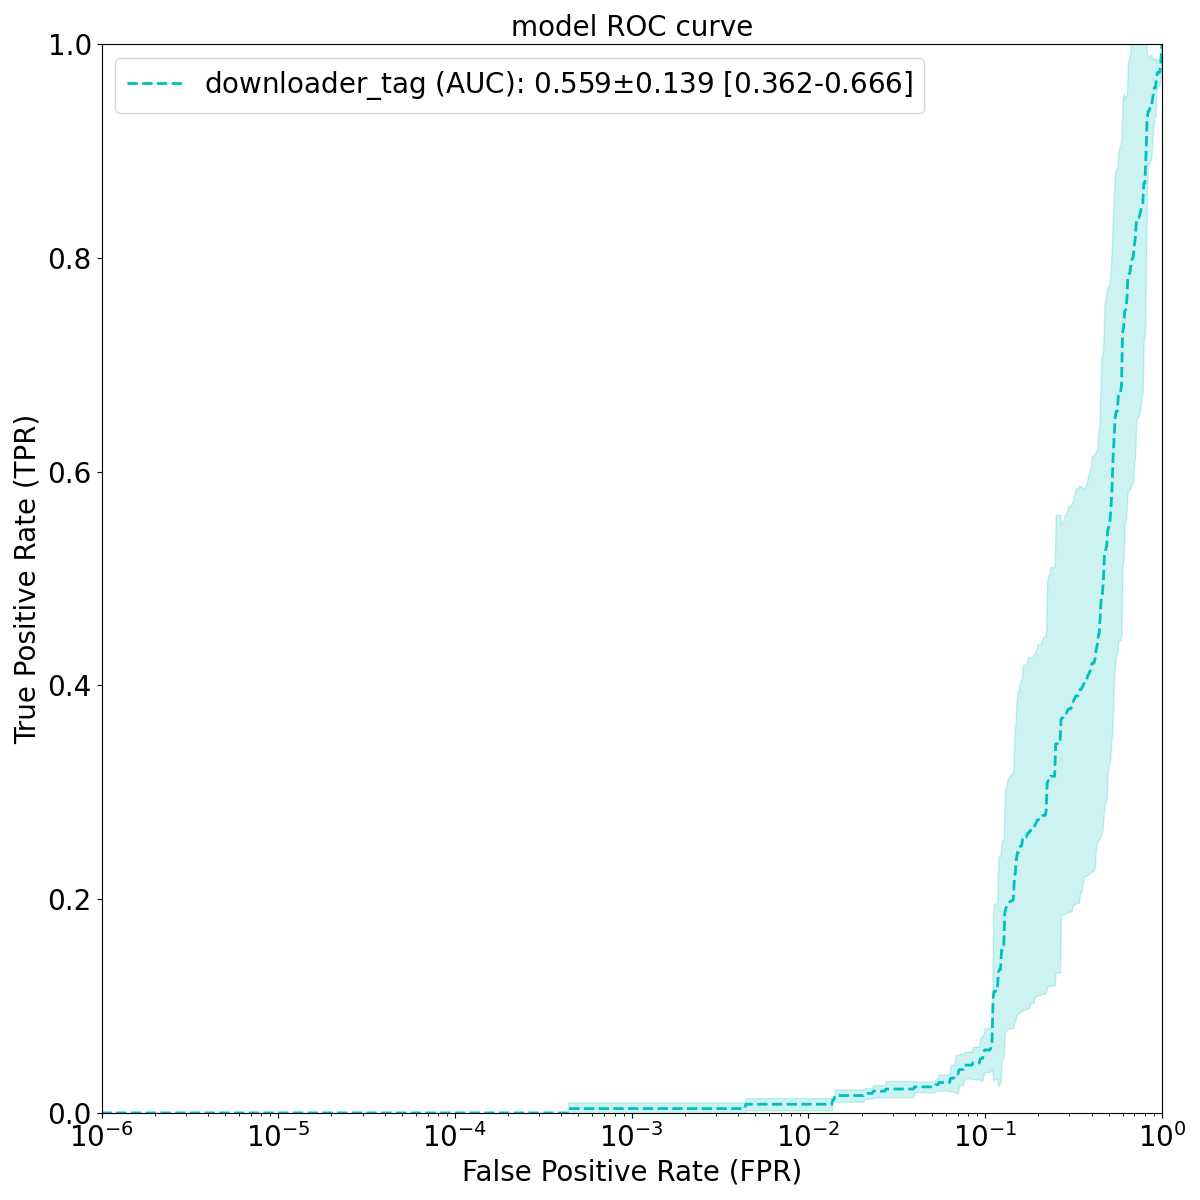
\includegraphics[width=0.6\textwidth]{./results/downloader_tag_roc_aloha.png}
        \vspace*{-0.2cm}
        \caption[Downloader Tag prediction task ALOHA ROC curve]{ROC curve and AUC statistics of \textBF{ALOHA} model for the \textbf{Downloader Tag}. The line represents the \textit{mean} TPR at a given FPR, while the shaded region represents the \textit{standard deviation}. Statistics were computed over \textBF{3} training runs, each with random parameter initialization.}
        \label{fig:downloaderTagRocAloha}
    \end{figure}
}

\newcommand{\downloaderTagRocJointEmbedding}{
    \begin{figure}[h!]
        \vspace*{-0.5cm}
        \centering
        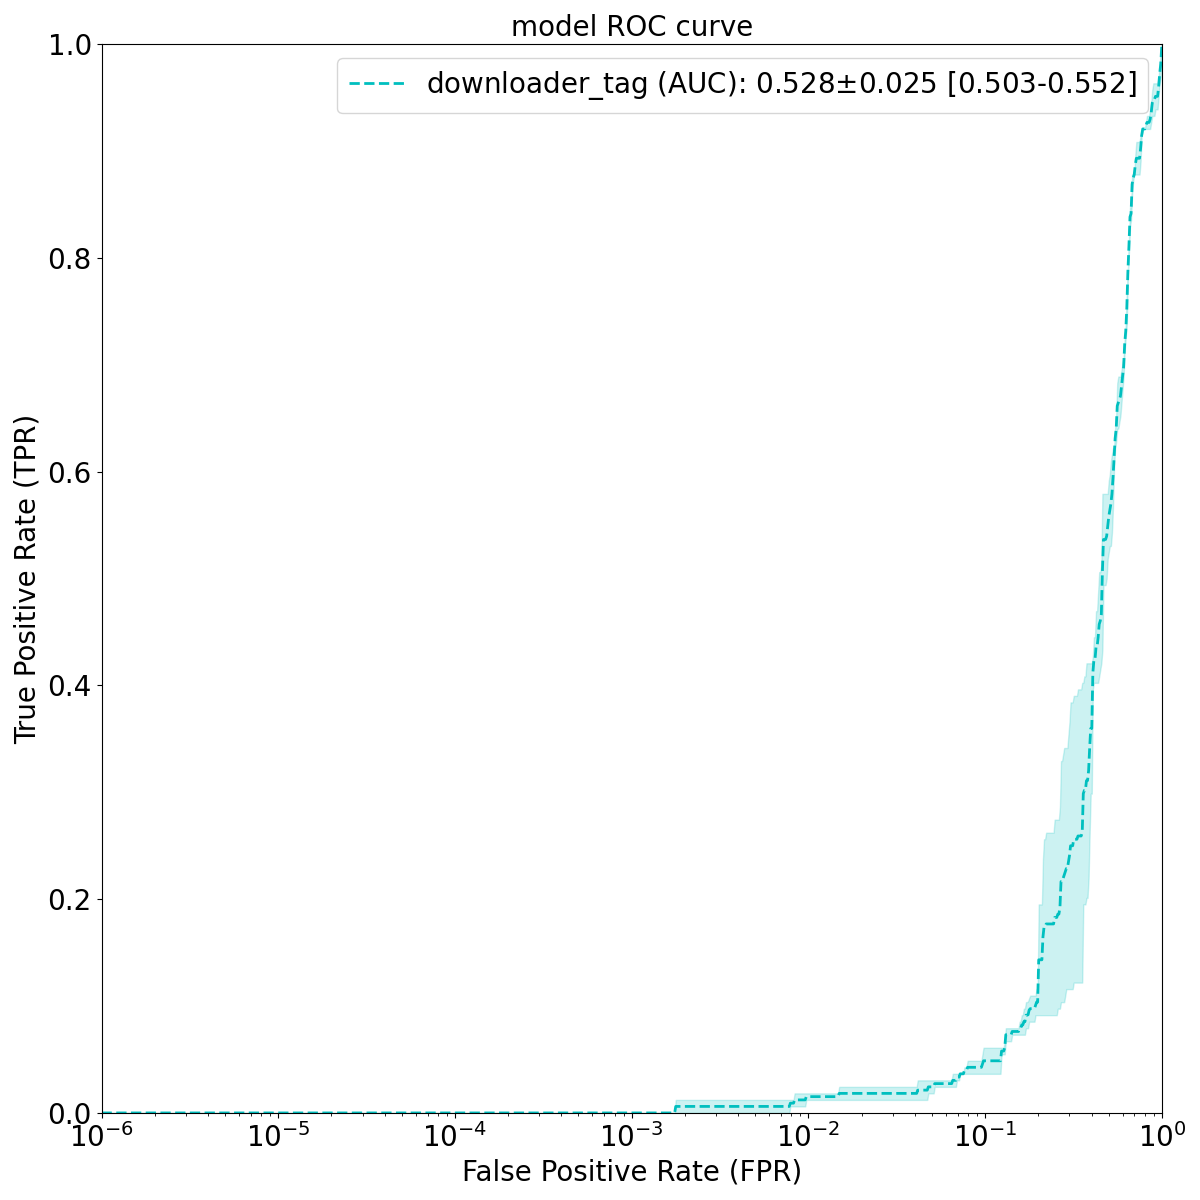
\includegraphics[width=0.6\textwidth]{./results/downloader_tag_roc_jointEmbedding.png}
        \vspace*{-0.2cm}
        \caption[Downloader Tag prediction task Joint Embedding ROC curve]{ROC curve and AUC statistics of \textBF{Joint Embedding} model for the \textbf{Downloader Tag}. The line represents the \textit{mean} TPR at a given FPR, while the shaded region represents the \textit{standard deviation}. Statistics were computed over \textBF{3} training runs, each with random parameter initialization.}
        \label{fig:downloaderTagRocJointEmbedding}
    \end{figure}
}

\newcommand{\downloaderTagRocProposedMethod}{
    \begin{figure}[h!]
        \vspace*{-0.5cm}
        \centering
        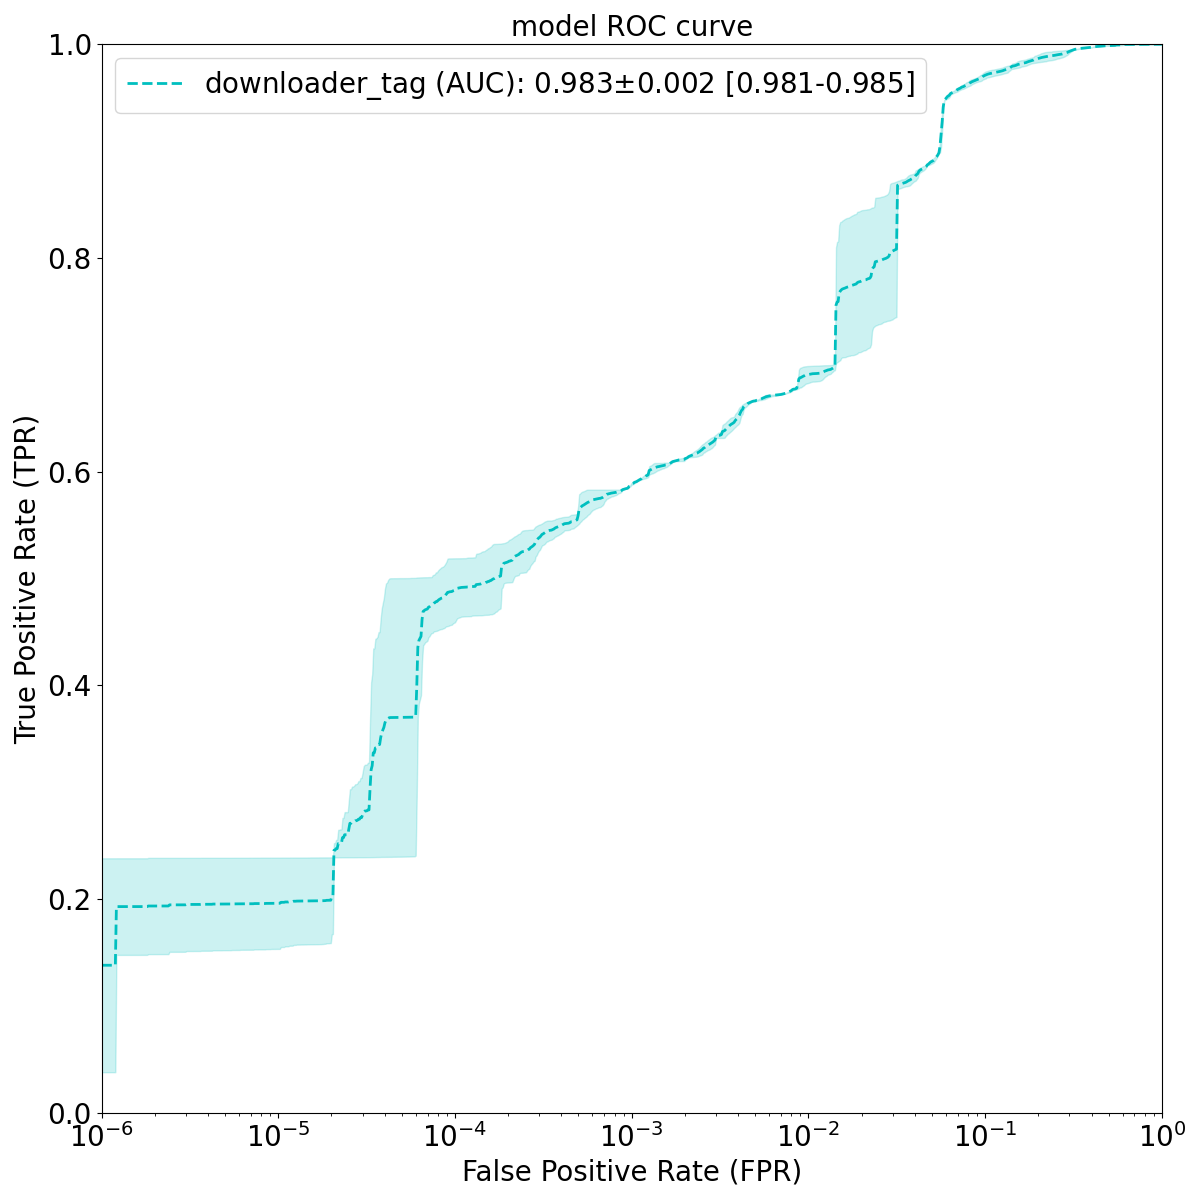
\includegraphics[width=0.6\textwidth]{./results/downloader_tag_roc_proposedModel.png}
        \vspace*{-0.2cm}
        \caption[Downloader Tag prediction task Proposed Model ROC curve]{ROC curve and AUC statistics of \textBF{Proposed Model} for the \textbf{Downloader Tag}. The line represents the \textit{mean} TPR at a given FPR, while the shaded region represents the \textit{standard deviation}. Statistics were computed over \textBF{3} training runs, each with random parameter initialization.}
        \label{fig:downloaderTagRocProposedModel}
    \end{figure}
}

%\newcommand{\dropperTagResultsAucTable}{
    \begin{table}[h!]
        \centering
        \begin{tabular}{|p{2,8cm}||P{2,2cm} P{2,2cm} P{2,2cm} P{2,2cm}|}
            \hline
            Dropper Tag & ALOHA\newline (M/B only) & ALOHA & Joint\newline Embedding & Proposed\newline Model \\
            \hline
            AUC-ROC & - & 0.972$\pm$0.001 & 0.973$\pm$0.001 & \textBF{0.976$\pm$0.001} \\
            \hline
        \end{tabular}
        \caption[Dropper Tag prediction task AUC-ROC results]{AUC-ROC (Area Under Curve) of the different models for the \textbf{Dropper Tag} prediction task. Results were aggregated over \textBF{3} training runs with different weight initializations and minibatch orderings. Best results are shown in \textbf{bold}.} \label{tab:dropperTag_auc}
    \end{table}
}

\newcommand{\dropperTagResultsAtFprTable}{
    \begin{center}
        \begin{longtable}[c]{|P{3,2cm}||P{1,8cm} P{1,8cm} P{1,8cm} P{1,8cm} P{1,8cm}|}
            \hline
            Dropper Tag & \multicolumn{5}{c|}{{FPR}} \\
            & $10^{-5}$ & $10^{-4}$ & $10^{-3}$ & $10^{-2}$ & $10^{-1}$ \\
            \hline
            \endfirsthead

            \caption*{\raggedright ...continued from previous page} \\
            \hline
            Dropper Tag & \multicolumn{5}{c|}{\textbf{FPR}} \\
            & $10^{-5}$ & $10^{-4}$ & $10^{-3}$ & $10^{-2}$ & $10^{-1}$ \\
            \hline
            \endhead

            \caption*{\raggedleft ...continued on next page} \\
            \endfoot

            \caption[Dropper Tag prediction task results]{Mean and standard deviation results (TPR, Accuracy, Recall, Precision and F1-Score) of the different models for the \textbf{Dropper Tag} prediction task at different \textbf{FPR}s (\textit{False Positive Rates}). Results were aggregated over \textBF{3} training runs with different weight initializations and minibatch orderings. Best results are shown in \textbf{bold}. Under \textbf{TPR} results are also presented the percentage reduction in mean detection error and in ROC curve standard deviation introduced by the \textit{Proposed Model} with respect to both \textit{ALOHA} model and \textit{Joint Embedding}.} \label{tab:dropperTag_results_at_fpr} \\
            \endlastfoot

            \multicolumn{6}{|c|}{\textbf{TPR}} \\
            \hline
            ALOHA (M/B only) & - & - & - & - & - \\
            ALOHA & 0.045$\pm$0.007 & 0.068$\pm$0.021 & 0.121$\pm$0.063 & 0.672$\pm$0.026 & 0.921$\pm$0.011 \\
            Joint Embedding & \textBF{0.118$\pm$0.078} & \textBF{0.159$\pm$0.132} & 0.179$\pm$0.131 & \textBF{0.730$\pm$0.011} & 0.910$\pm$0.015 \\
            Proposed Model & 0.042$\pm$0.020 & 0.128$\pm$0.051 & \textBF{0.206$\pm$0.076} & 0.724$\pm$0.016 & \textBF{0.933$\pm$0.015} \\
            \hline
            Error Reduction wrt\newline ALOHA (M/B only) & - & - & - & - & - \\
            Error Reduction wrt\newline ALOHA & -0.3\% & 6.4\% & 9.7\% & 15.9\% & 15.2\% \\
            Error Reduction wrt\newline Joint Embedding & -8.6\% & -3.7\% & 3.3\% & -2.2\% & 25.6\% \\
            \hline
            Std Reduction wrt\newline ALOHA (M/B only) & - & - & - & - & - \\
            Std Reduction wrt\newline ALOHA & -185.7\% & -142.9\% & -20.6\% & 38.5\% & -36.4\% \\
            Std Reduction wrt\newline Joint Embedding & 74.4\% & 61.4\% & 42.0\% & -45.5\% & 0.0\% \\
            \hline
            \multicolumn{6}{|c|}{\textbf{Accuracy}} \\
            \hline
            ALOHA (M/B only) & - & - & - & - & - \\
            ALOHA & 0.878$\pm$0.001 & 0.881$\pm$0.003 & 0.887$\pm$0.008 & 0.949$\pm$0.003 & 0.903$\pm$0.001 \\
            Joint Embedding & \textBF{0.887$\pm$0.010} & \textBF{0.893$\pm$0.017} & 0.894$\pm$0.017 & \textBF{0.957$\pm$0.001} & 0.901$\pm$0.002 \\
            Proposed Model & 0.878$\pm$0.003 & 0.889$\pm$0.007 & \textBF{0.898$\pm$0.010} & 0.956$\pm$0.002 & \textBF{0.904$\pm$0.002} \\
            \hline
            \multicolumn{6}{|c|}{\textbf{Recall}} \\
            \hline
            ALOHA (M/B only) & - & - & - & - & - \\
            ALOHA & 0.045$\pm$0.007 & 0.068$\pm$0.021 & 0.121$\pm$0.063 & 0.672$\pm$0.026 & 0.921$\pm$0.011 \\
            Joint Embedding & \textBF{0.118$\pm$0.078} & \textBF{0.159$\pm$0.132} & 0.179$\pm$0.131 & \textBF{0.730$\pm$0.011} & 0.910$\pm$0.015 \\
            Proposed Model & 0.042$\pm$0.020 & 0.128$\pm$0.051 & \textBF{0.206$\pm$0.076} & 0.724$\pm$0.016 & \textBF{0.933$\pm$0.015} \\
            \hline
            \multicolumn{6}{|c|}{\textbf{Precision}} \\
            \hline
            ALOHA (M/B only) & - & - & - & - & - \\
            ALOHA & \textBF{0.999$\pm$0.000} & 0.989$\pm$0.004 & 0.931$\pm$0.035 & 0.908$\pm$0.003 & 0.574$\pm$0.003 \\
            Joint Embedding & 0.999$\pm$0.001 & 0.992$\pm$0.005 & 0.944$\pm$0.029 & \textBF{0.914$\pm$0.001} & 0.571$\pm$0.004 \\
            Proposed Model & 0.998$\pm$0.001 & \textBF{0.994$\pm$0.002} & \textBF{0.963$\pm$0.015} & 0.914$\pm$0.002 & \textBF{0.577$\pm$0.004} \\
            \hline
            \multicolumn{6}{|c|}{\textbf{F1 Score}} \\
            \hline
            ALOHA (M/B only) & - & - & - & - & - \\
            ALOHA & 0.086$\pm$0.013 & 0.127$\pm$0.038 & 0.210$\pm$0.098 & 0.772$\pm$0.019 & 0.707$\pm$0.005 \\
            Joint Embedding & \textBF{0.203$\pm$0.121} & \textBF{0.253$\pm$0.186} & 0.282$\pm$0.177 & \textBF{0.812$\pm$0.007} & 0.702$\pm$0.007 \\
            Proposed Model & 0.080$\pm$0.036 & 0.222$\pm$0.079 & \textBF{0.332$\pm$0.106} & 0.808$\pm$0.011 & \textBF{0.713$\pm$0.007} \\
            \hline
        \end{longtable}
    \end{center}
}

\newcommand{\dropperTagResultsSummaryTable}{
    \begin{table}[h!]
        \centering
        \begin{tabular}{|P{3,2cm}||P{1,8cm} P{1,8cm} P{1,8cm} P{1,8cm} P{1,8cm}|}
            \hline
            \multicolumn{6}{|c|}{Dropper Tag (at FPR $=1\%$)} \\
            \hline
            Model & TPR & Accuracy & Precision & Recall & F1 score \\
            \hline
            ALOHA (M/B only) & - & - & - & - & - \\
            ALOHA & 0.672$\pm$0.026 & 0.949$\pm$0.003 & 0.908$\pm$0.003 & 0.672$\pm$0.026 & 0.772$\pm$0.019 \\
            Joint Embedding & \textBF{0.730$\pm$0.011} & \textBF{0.957$\pm$0.001} & \textBF{0.914$\pm$0.001} & \textBF{0.730$\pm$0.011} & \textBF{0.812$\pm$0.007} \\
            Proposed Model & 0.724$\pm$0.016 & 0.956$\pm$0.002 & 0.914$\pm$0.002 & 0.724$\pm$0.016 & 0.808$\pm$0.011 \\
            \hline
        \end{tabular}
        \caption[Summary of Dropper Tag prediction task results]{Summary of the mean and standard deviation results of the different models for the \textbf{Dropper Tag} prediction task at \textbf{FPR} $=1\%$. Results were aggregated over \textBF{3} training runs with different weight initializations and minibatch orderings. Best results are shown in \textbf{bold}.} \label{tab:dropperTag_result_summary}
    \end{table}
}

\newcommand{\dropperTagRocAlohaMB}{
    \begin{figure}[h!]
        \vspace*{-0.5cm}
        \centering
        \includegraphics[width=0.6\textwidth]{./results/dropper_tag_roc_alohaMB.png}
        \vspace*{-0.2cm}
        \caption[Dropper Tag prediction task ALOHA (M/B only) ROC curve]{ROC curve and AUC statistics of \textBF{ALOHA (M/B only)} model for the \textbf{Dropper Tag}. The line represents the \textit{mean} TPR at a given FPR, while the shaded region represents the \textit{standard deviation}. Statistics were computed over \textBF{3} training runs, each with random parameter initialization.}
        \label{fig:dropperTagRocAlohaMB}
    \end{figure}
}

\newcommand{\dropperTagRocAloha}{
    \begin{figure}[h!]
        \vspace*{-0.5cm}
        \centering
        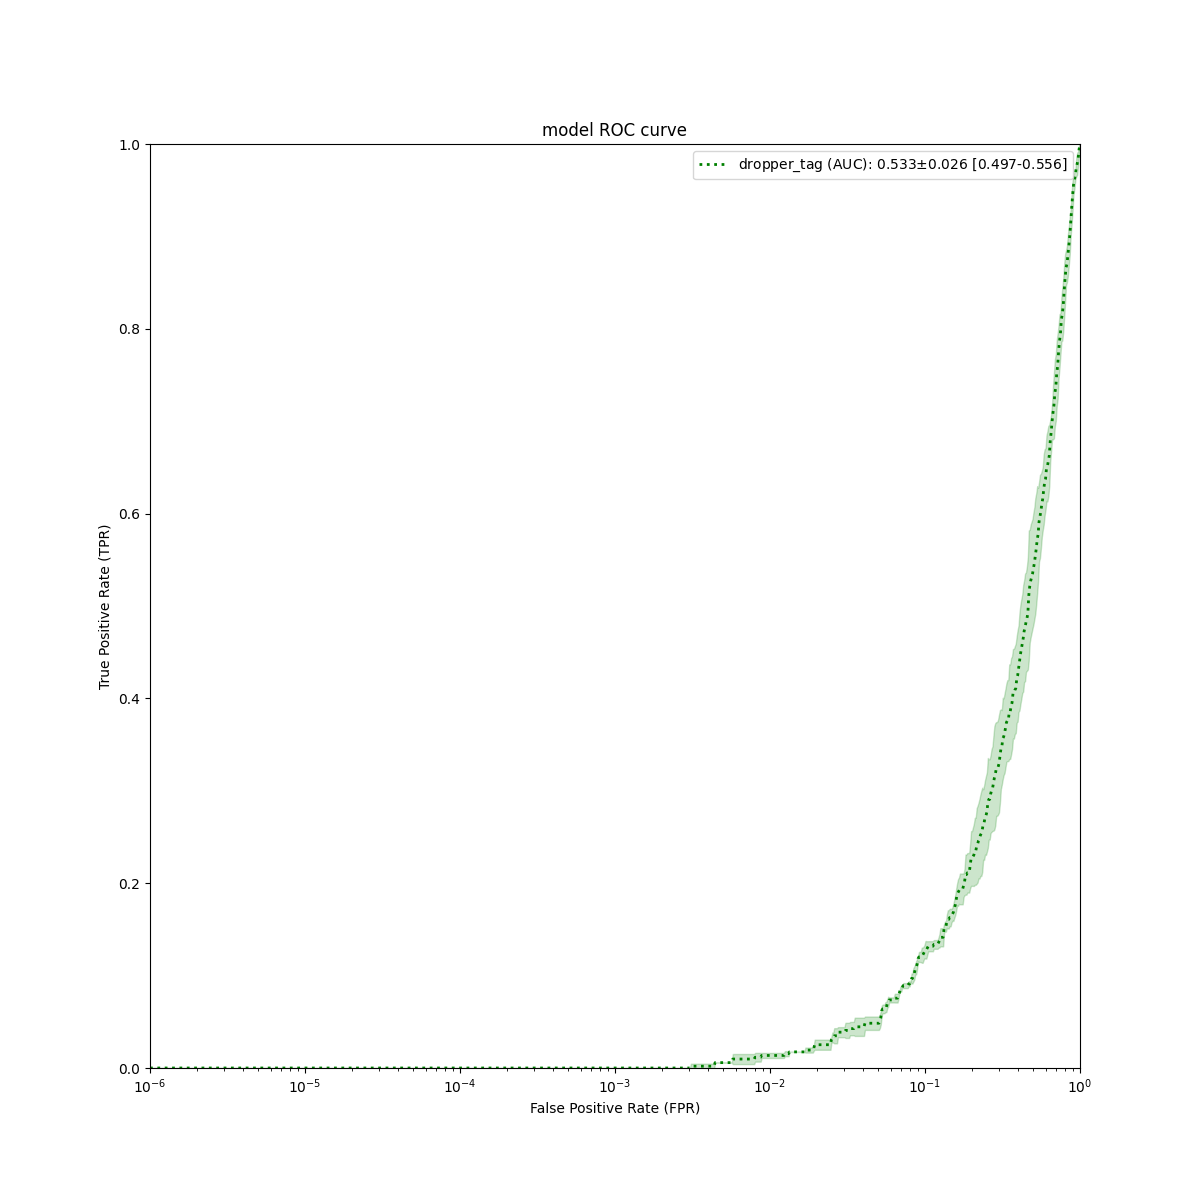
\includegraphics[width=0.6\textwidth]{./results/dropper_tag_roc_aloha.png}
        \vspace*{-0.2cm}
        \caption[Dropper Tag prediction task ALOHA ROC curve]{ROC curve and AUC statistics of \textBF{ALOHA} model for the \textbf{Dropper Tag}. The line represents the \textit{mean} TPR at a given FPR, while the shaded region represents the \textit{standard deviation}. Statistics were computed over \textBF{3} training runs, each with random parameter initialization.}
        \label{fig:dropperTagRocAloha}
    \end{figure}
}

\newcommand{\dropperTagRocJointEmbedding}{
    \begin{figure}[h!]
        \vspace*{-0.5cm}
        \centering
        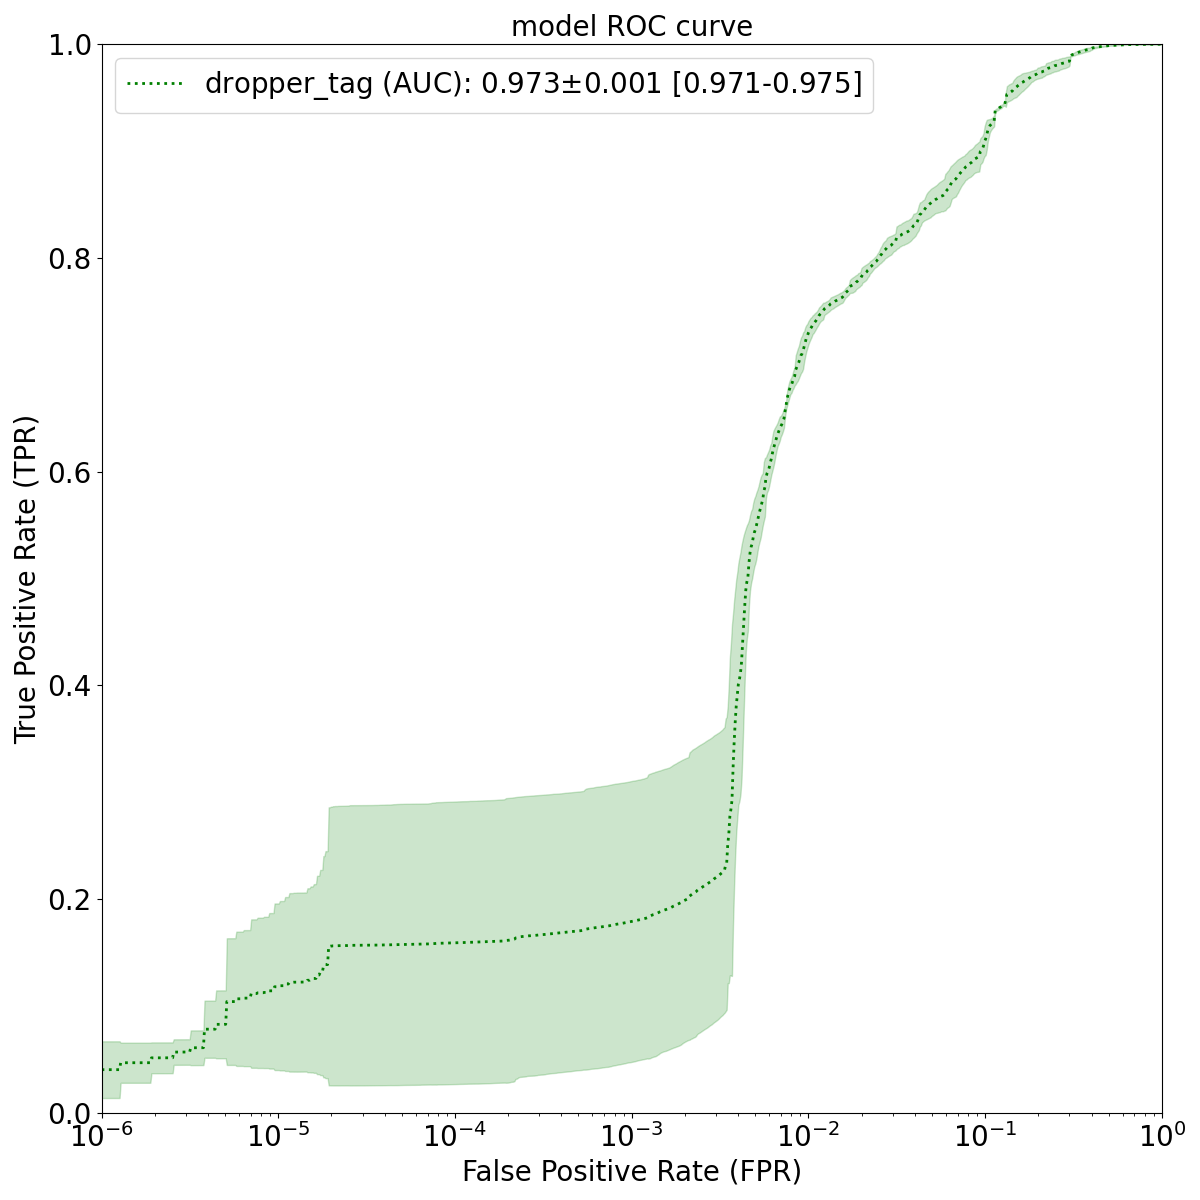
\includegraphics[width=0.6\textwidth]{./results/dropper_tag_roc_jointEmbedding.png}
        \vspace*{-0.2cm}
        \caption[Dropper Tag prediction task Joint Embedding ROC curve]{ROC curve and AUC statistics of \textBF{Joint Embedding} model for the \textbf{Dropper Tag}. The line represents the \textit{mean} TPR at a given FPR, while the shaded region represents the \textit{standard deviation}. Statistics were computed over \textBF{3} training runs, each with random parameter initialization.}
        \label{fig:dropperTagRocJointEmbedding}
    \end{figure}
}

\newcommand{\dropperTagRocProposedMethod}{
    \begin{figure}[h!]
        \vspace*{-0.5cm}
        \centering
        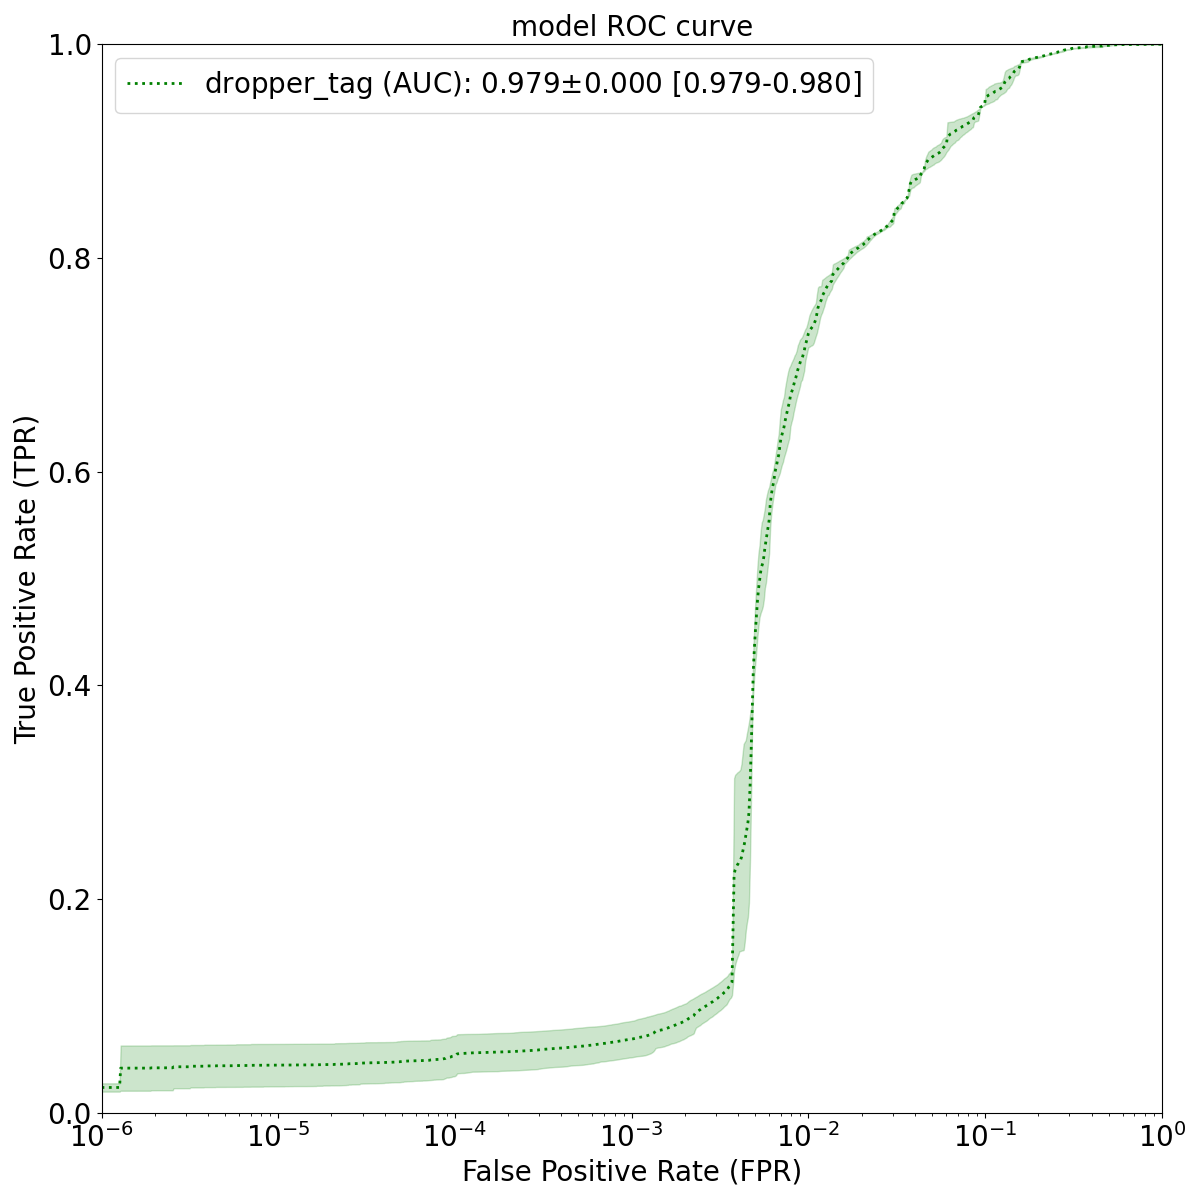
\includegraphics[width=0.6\textwidth]{./results/dropper_tag_roc_proposedModel.png}
        \vspace*{-0.2cm}
        \caption[Dropper Tag prediction task Proposed Model ROC curve]{ROC curve and AUC statistics of \textBF{Proposed Model} for the \textbf{Dropper Tag}. The line represents the \textit{mean} TPR at a given FPR, while the shaded region represents the \textit{standard deviation}. Statistics were computed over \textBF{3} training runs, each with random parameter initialization.}
        \label{fig:dropperTagRocProposedModel}
    \end{figure}
}

%\newcommand{\fileInfectorTagResultsAucTable}{
    \begin{table}[H]
        \centering
        \begin{tabular}{|p{2,8cm}||P{2,2cm} P{2,2cm} P{2,2cm} P{2,2cm}|}
            \hline
            File-infector Tag & ALOHA\newline (M/B only) & ALOHA & Joint\newline Embedding & Proposed\newline Model \\
            \hline
            AUC-ROC & - & 0.982$\pm$0.002 & 0.983$\pm$0.001 & \textBF{0.986$\pm$0.001} \\
            \hline
        \end{tabular}
        \caption{AUC-ROC (Area Under Curve) of the different models for the \textbf{File-infector Tag} prediction task. Results were aggregated over \textBF{3} training runs with different weight initializations and minibatch orderings. Best results are shown in \textbf{bold}.} \label{tab:fileInfectorTag_auc}
    \end{table}
}

\newcommand{\fileInfectorTagResultsAtFprTable}{
    \begin{center}
        \begin{longtable}[c]{|P{3,2cm}||P{1,8cm} P{1,8cm} P{1,8cm} P{1,8cm} P{1,8cm}|}
            \hline
            File-infector Tag & \multicolumn{5}{c|}{{FPR}} \\
            & $10^{-5}$ & $10^{-4}$ & $10^{-3}$ & $10^{-2}$ & $10^{-1}$ \\
            \hline
            \endfirsthead

            \caption*{\raggedright ...continued from previous page} \\
            \hline
            File-infector Tag & \multicolumn{5}{c|}{\textbf{FPR}} \\
            & $10^{-5}$ & $10^{-4}$ & $10^{-3}$ & $10^{-2}$ & $10^{-1}$ \\
            \hline
            \endhead

            \caption*{\raggedleft ...continued on next page} \\
            \endfoot

            \caption{Mean and standard deviation results (TPR, Accuracy, Recall, Precision and F1-Score) of the different models for the \textbf{File-infector Tag} prediction task at different \textbf{FPR}s (\textit{False Positive Rates}). Results were aggregated over \textBF{3} training runs with different weight initializations and minibatch orderings. Best results are shown in \textbf{bold}. Under \textbf{TPR} results are also presented the percentage reduction in mean detection error and in ROC curve standard deviation introduced by the \textit{Proposed Model} with respect to both \textit{ALOHA} model and \textit{Joint Embedding}.} \label{tab:fileInfectorTag_results_at_fpr} \\
            \endlastfoot

            \multicolumn{6}{|c|}{\textbf{TPR}} \\
            \hline
            ALOHA (M/B only) & - & - & - & - & - \\
            ALOHA & \textBF{0.375$\pm$0.199} & 0.481$\pm$0.173 & 0.799$\pm$0.018 & 0.851$\pm$0.008 & 0.946$\pm$0.013 \\
            Joint Embedding & 0.294$\pm$0.166 & \textBF{0.541$\pm$0.131} & 0.797$\pm$0.025 & 0.857$\pm$0.009 & 0.952$\pm$0.013 \\
            Proposed Model & 0.360$\pm$0.155 & 0.532$\pm$0.060 & \textBF{0.829$\pm$0.022} & \textBF{0.872$\pm$0.011} & \textBF{0.956$\pm$0.013} \\
            \hline
            Error Reduction wrt\newline ALOHA (M/B only) & - & - & - & - & - \\
            Error Reduction wrt\newline ALOHA & -2.4\% & 9.8\% & 14.9\% & 14.1\% & 18.5\% \\
            Error Reduction wrt\newline Joint Embedding & 9.3\% & -2.0\% & 15.8\% & 10.5\% & 8.3\% \\
            \hline
            Std Reduction wrt\newline ALOHA (M/B only) & - & - & - & - & - \\
            Std Reduction wrt\newline ALOHA & 22.1\% & 65.3\% & -22.2\% & -37.5\% & 0.0\% \\
            Std Reduction wrt\newline Joint Embedding & 6.6\% & 54.2\% & 12.0\% & -22.2\% & 0.0\% \\
            \hline
            \multicolumn{6}{|c|}{\textbf{Accuracy}} \\
            \hline
            ALOHA (M/B only) & - & - & - & - & - \\
            ALOHA & \textBF{0.899$\pm$0.032} & 0.916$\pm$0.028 & 0.967$\pm$0.003 & 0.968$\pm$0.001 & 0.907$\pm$0.002 \\
            Joint Embedding & 0.886$\pm$0.027 & \textBF{0.926$\pm$0.021} & 0.966$\pm$0.004 & 0.969$\pm$0.001 & 0.908$\pm$0.002 \\
            Proposed Model & 0.897$\pm$0.025 & 0.924$\pm$0.010 & \textBF{0.972$\pm$0.004} & \textBF{0.971$\pm$0.002} & \textBF{0.909$\pm$0.002} \\
            \hline
            \multicolumn{6}{|c|}{\textbf{Recall}} \\
            \hline
            ALOHA (M/B only) & - & - & - & - & - \\
            ALOHA & \textBF{0.374$\pm$0.199} & 0.481$\pm$0.173 & 0.799$\pm$0.018 & 0.851$\pm$0.008 & 0.946$\pm$0.013 \\
            Joint Embedding & 0.294$\pm$0.166 & \textBF{0.541$\pm$0.131} & 0.797$\pm$0.025 & 0.857$\pm$0.009 & 0.952$\pm$0.013 \\
            Proposed Model & 0.360$\pm$0.155 & 0.531$\pm$0.060 & \textBF{0.829$\pm$0.022} & \textBF{0.872$\pm$0.011} & \textBF{0.956$\pm$0.013} \\
            \hline
            \multicolumn{6}{|c|}{\textbf{Precision}} \\
            \hline
            ALOHA (M/B only) & - & - & - & - & - \\
            ALOHA & \textBF{1.000$\pm$0.000} & \textBF{0.999$\pm$0.000} & \textBF{0.994$\pm$0.000} & 0.943$\pm$0.000 & 0.646$\pm$0.003 \\
            Joint Embedding & \textBF{1.000$\pm$0.000} & \textBF{0.999$\pm$0.000} & \textBF{0.994$\pm$0.000} & 0.943$\pm$0.001 & 0.647$\pm$0.003 \\
            Proposed Model & \textBF{1.000$\pm$0.000} & \textBF{0.999$\pm$0.000} & \textBF{0.994$\pm$0.000} & \textBF{0.944$\pm$0.001} & \textBF{0.648$\pm$0.003} \\
            \hline
            \multicolumn{6}{|c|}{\textbf{F1 Score}} \\
            \hline
            ALOHA (M/B only) & - & - & - & - & - \\
            ALOHA & \textBF{0.517$\pm$0.195} & 0.632$\pm$0.150 & 0.886$\pm$0.011 & 0.894$\pm$0.004 & 0.767$\pm$0.006 \\
            Joint Embedding & 0.427$\pm$0.216 & 0.692$\pm$0.117 & 0.884$\pm$0.015 & 0.898$\pm$0.005 & 0.771$\pm$0.007 \\
            Proposed Model & 0.509$\pm$0.180 & \textBF{0.692$\pm$0.053} & \textBF{0.904$\pm$0.013} & \textBF{0.907$\pm$0.006} & \textBF{0.772$\pm$0.006} \\
            \hline
        \end{longtable}
    \end{center}
}

\newcommand{\fileInfectorTagResultsSummaryTable}{
    \begin{table}[H]
        \centering
        \begin{tabular}{|P{3,2cm}||P{1,8cm} P{1,8cm} P{1,8cm} P{1,8cm} P{1,8cm}|}
            \hline
            \multicolumn{6}{|c|}{File-infector Tag (at FPR $=1\%$)} \\
            \hline
            Model & TPR & Accuracy & Precision & Recall & F1 score \\
            \hline
            ALOHA (M/B only) & - & - & - & - & - \\
            ALOHA & 0.851$\pm$0.008 & 0.968$\pm$0.001 & 0.943$\pm$0.000 & 0.851$\pm$0.008 & 0.894$\pm$0.004 \\
            Joint Embedding & 0.857$\pm$0.009 & 0.969$\pm$0.001 & 0.943$\pm$0.001 & 0.857$\pm$0.009 & 0.898$\pm$0.005 \\
            Proposed Model & \textBF{0.872$\pm$0.011} & \textBF{0.971$\pm$0.002} & \textBF{0.944$\pm$0.001} & \textBF{0.872$\pm$0.011} & \textBF{0.907$\pm$0.006} \\
            \hline
        \end{tabular}
        \caption{Summary of the mean and standard deviation results of the different models for the \textbf{File-infector Tag} prediction task at \textbf{FPR} $=1\%$. Results were aggregated over \textBF{3} training runs with different weight initializations and minibatch orderings. Best results are shown in \textbf{bold}.} \label{tab:fileInfectorTag_result_summary}
    \end{table}
}

\newcommand{\fileInfectorTagRocAlohaMB}{
    \begin{figure}[H]
        \vspace*{-0.5cm}
        \centering
        \includegraphics[width=0.6\textwidth]{./results/file_infector_tag_roc_alohaMB.png}
        \vspace*{-0.2cm}
        \caption{ROC curve and AUC statistics of \textBF{ALOHA (M/B only)} model for the \textbf{File-infector Tag}. The line represents the \textit{mean} TPR at a given FPR, while the shaded region represents the \textit{standard deviation}. Statistics were computed over \textBF{3} training runs, each with random parameter initialization.}
        \label{fig:fileInfectorTagRocAlohaMB}
    \end{figure}
}

\newcommand{\fileInfectorTagRocAloha}{
    \begin{figure}[H]
        \vspace*{-0.5cm}
        \centering
        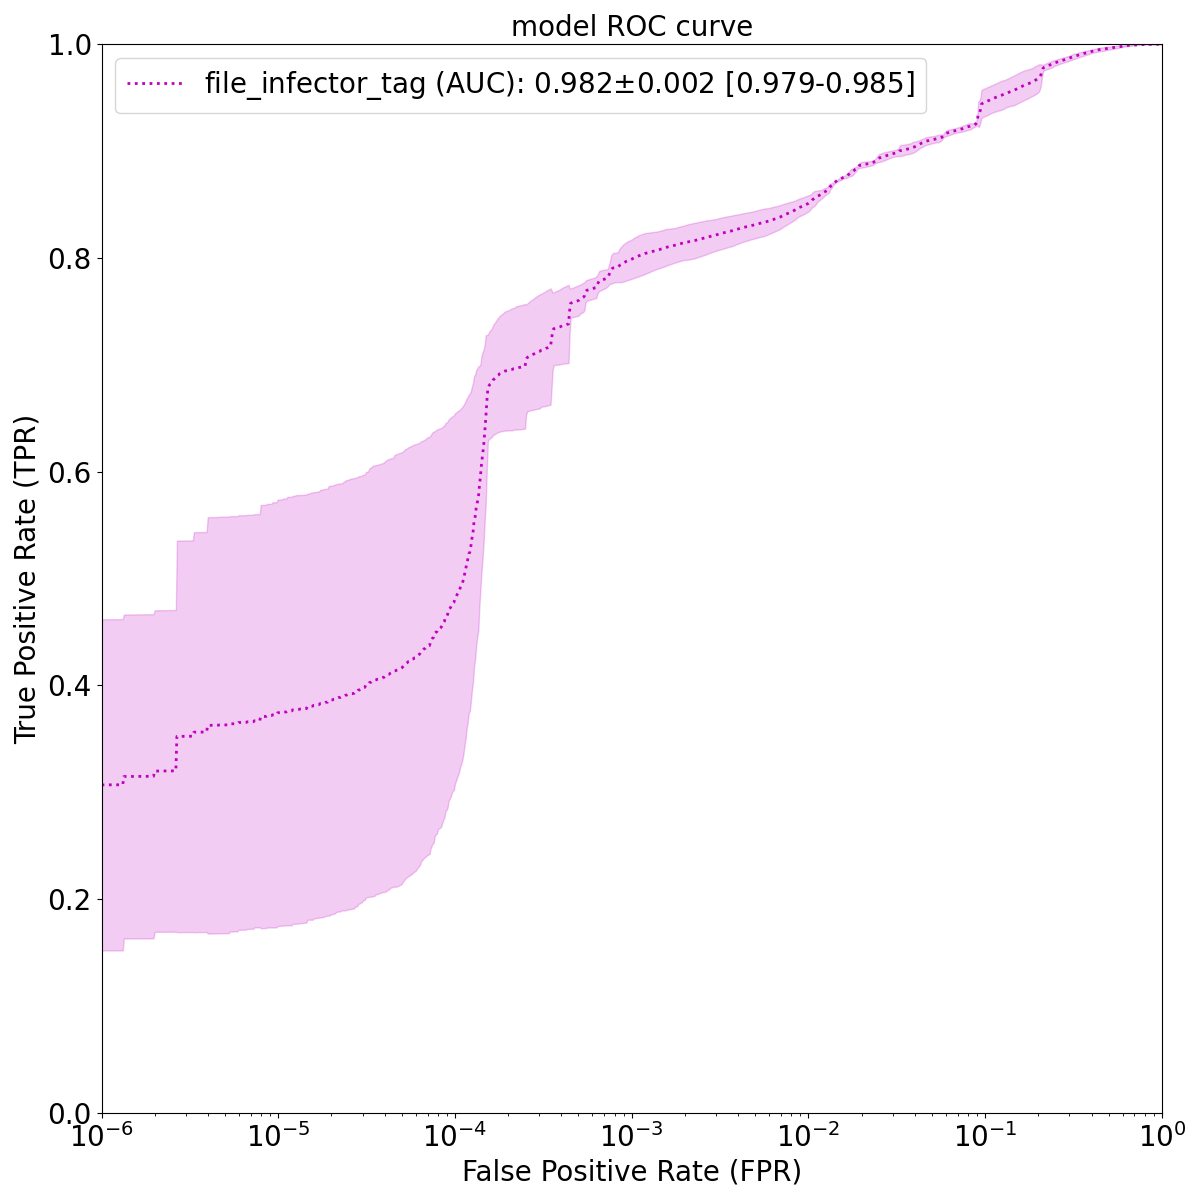
\includegraphics[width=0.6\textwidth]{./results/file_infector_tag_roc_aloha.png}
        \vspace*{-0.2cm}
        \caption{ROC curve and AUC statistics of \textBF{ALOHA} model for the \textbf{File-infector Tag}. The line represents the \textit{mean} TPR at a given FPR, while the shaded region represents the \textit{standard deviation}. Statistics were computed over \textBF{3} training runs, each with random parameter initialization.}
        \label{fig:fileInfectorTagRocAloha}
    \end{figure}
}

\newcommand{\fileInfectorTagRocJointEmbedding}{
    \begin{figure}[H]
        \vspace*{-0.5cm}
        \centering
        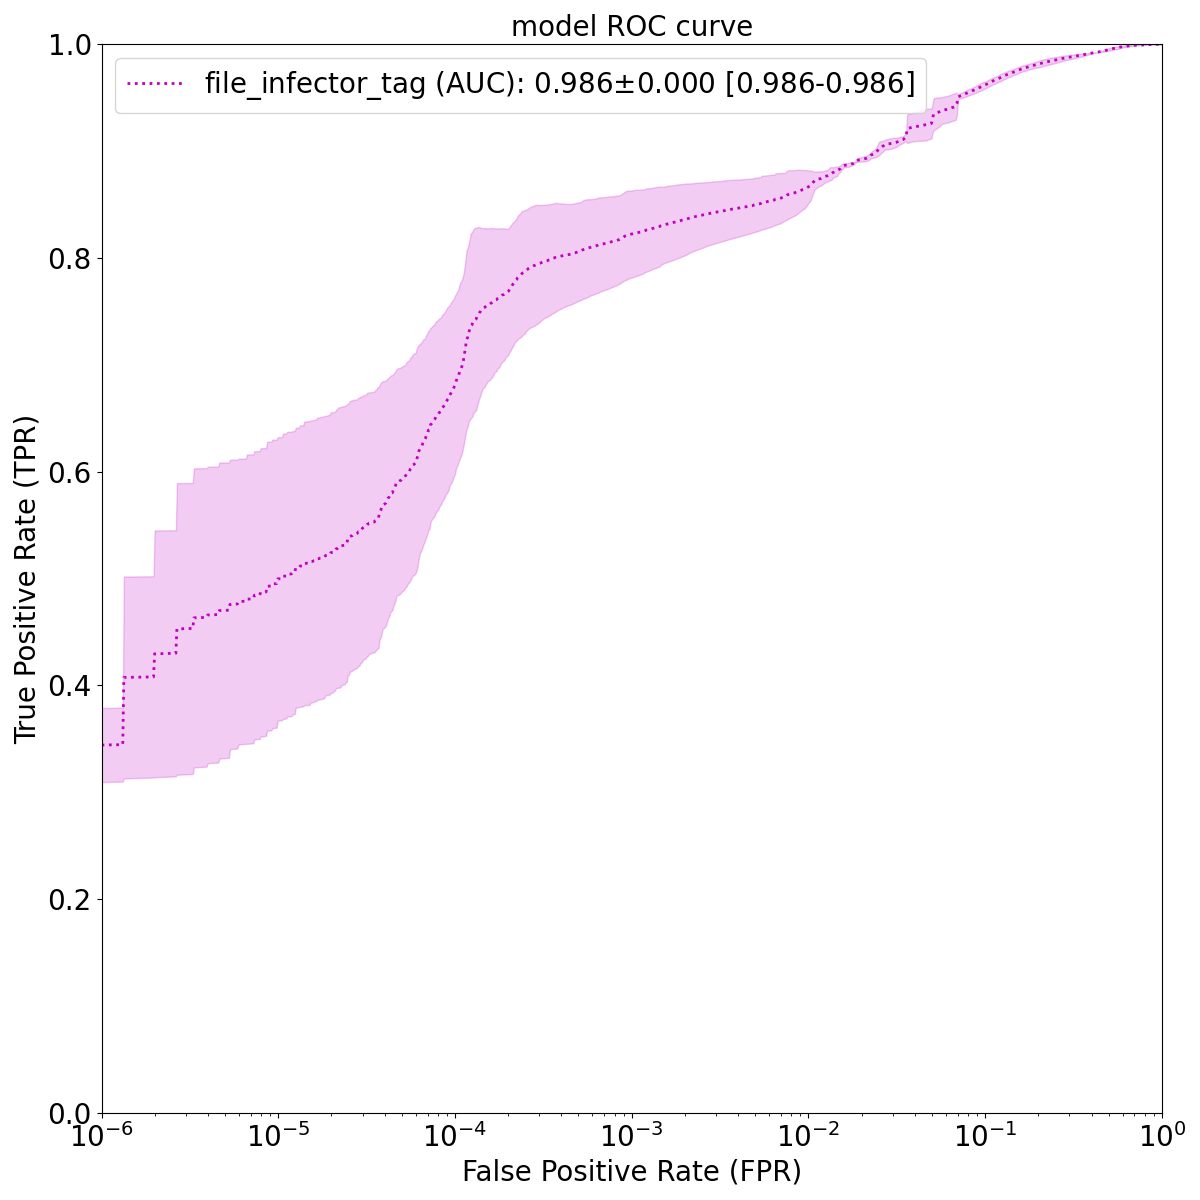
\includegraphics[width=0.6\textwidth]{./results/file_infector_tag_roc_jointEmbedding.png}
        \vspace*{-0.2cm}
        \caption{ROC curve and AUC statistics of \textBF{Joint Embedding} model for the \textbf{File-infector Tag}. The line represents the \textit{mean} TPR at a given FPR, while the shaded region represents the \textit{standard deviation}. Statistics were computed over \textBF{3} training runs, each with random parameter initialization.}
        \label{fig:fileInfectorTagRocJointEmbedding}
    \end{figure}
}

\newcommand{\fileInfectorTagRocProposedMethod}{
    \begin{figure}[H]
        \vspace*{-0.5cm}
        \centering
        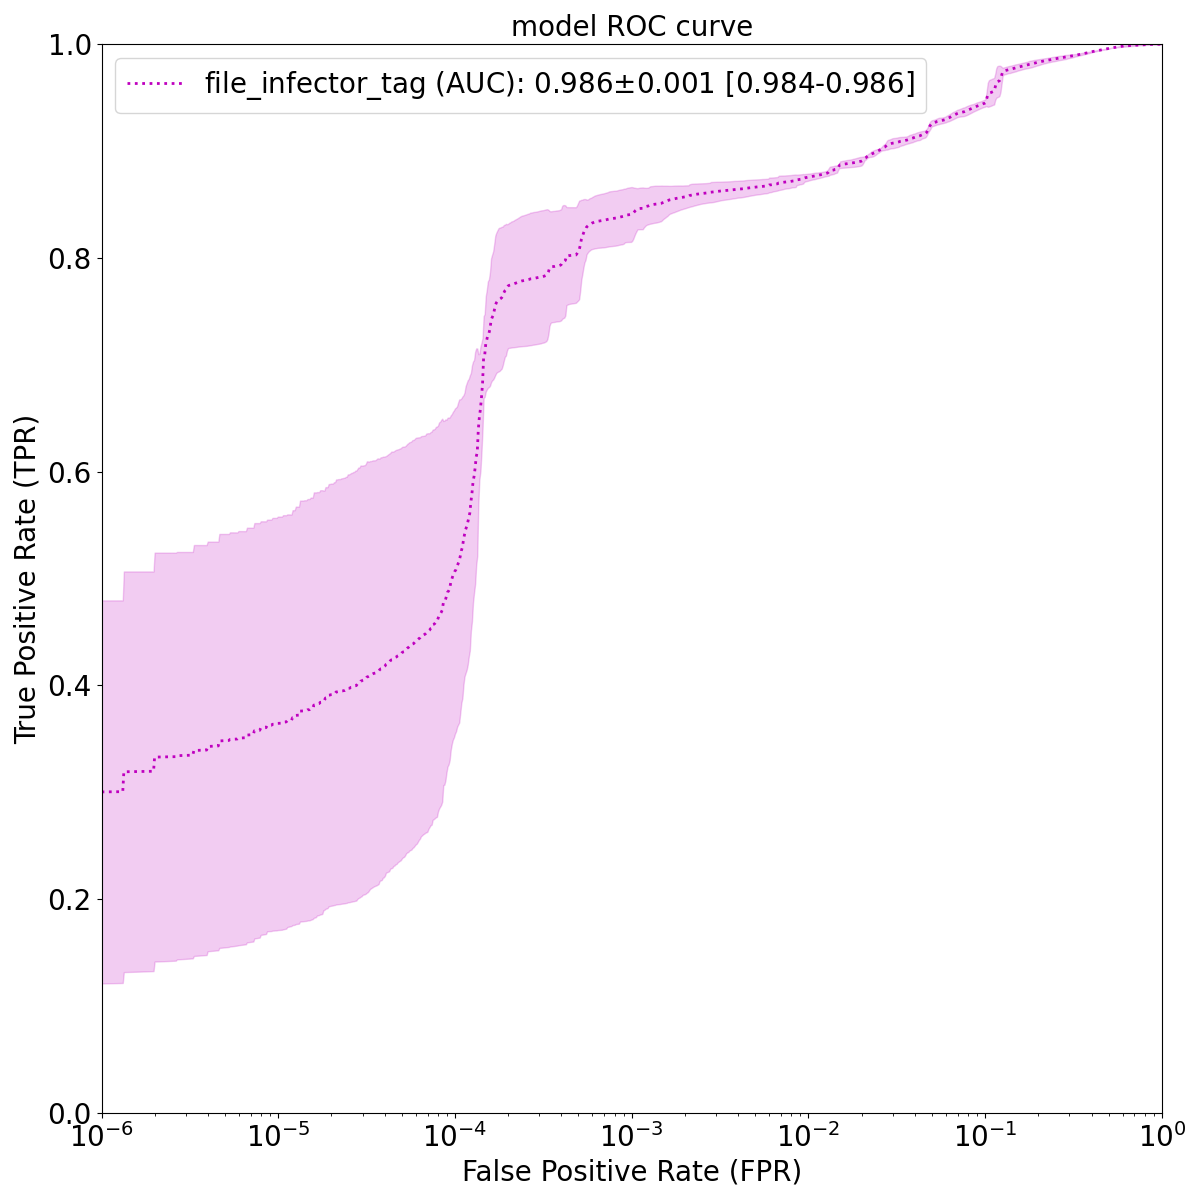
\includegraphics[width=0.6\textwidth]{./results/file_infector_tag_roc_proposedModel.png}
        \vspace*{-0.2cm}
        \caption{ROC curve and AUC statistics of \textBF{Proposed Model} for the \textbf{File-infector Tag}. The line represents the \textit{mean} TPR at a given FPR, while the shaded region represents the \textit{standard deviation}. Statistics were computed over \textBF{3} training runs, each with random parameter initialization.}
        \label{fig:fileInfectorTagRocProposedModel}
    \end{figure}
}

%\newcommand{\flooderTagResultsAucTable}{
    \begin{table}[H]
        \centering
        \begin{tabular}{|p{2,8cm}||p{2,8cm} p{2,8cm} p{2,8cm}|}
            \hline
            Flooder Tag & ALOHA & Joint Embedding & Proposed Model \\
            \hline
            AUC-ROC & \textBF{0.596$\pm$0.108} & 0.390$\pm$0.206 & 0.564$\pm$0.110 \\
            \hline
        \end{tabular}
        \caption{AUC-ROC (Area Under Curve) of the different models for the \textbf{Flooder Tag} prediction task. Results were aggregated over \textBF{3} training runs with different weight initializations and minibatch orderings. Best results are shown in \textbf{bold}.} \label{tab:flooderTag_auc}
    \end{table}
}

\newcommand{\flooderTagResultsAtFprTable}{
    \begin{center}
        \begin{longtable}[c]{|p{3,2cm}||p{1,8cm} p{1,8cm} p{1,8cm} p{1,8cm} p{1,8cm}|}
            \hline
            Flooder Tag & \multicolumn{5}{c|}{{FPR}} \\
            & $10^{-5}$ & $10^{-4}$ & $10^{-3}$ & $10^{-2}$ & $10^{-1}$ \\
            \hline
            \endfirsthead

            \caption*{\raggedright ...continued from previous page} \\
            \hline
            Flooder Tag & \multicolumn{5}{c|}{\textbf{FPR}} \\
            & $10^{-5}$ & $10^{-4}$ & $10^{-3}$ & $10^{-2}$ & $10^{-1}$ \\
            \hline
            \endhead

            \caption*{\raggedleft ...continued on next page} \\
            \endfoot

            \caption{Mean and standard deviation results (TPR, Accuracy, Recall, Precision and F1-Score) of the different models for the \textbf{Flooder Tag} prediction task at different \textbf{FPR}s (\textit{False Positive Rates}). Results were aggregated over \textBF{3} training runs with different weight initializations and minibatch orderings. Best results are shown in \textbf{bold}. Under \textbf{TPR} results are also presented the percentage reduction in mean detection error and in ROC curve standard deviation introduced by the \textit{Proposed Model} with respect to both \textit{ALOHA} model and \textit{Joint Embedding}.} \label{tab:flooderTag_results_at_fpr} \\
            \endlastfoot

            \multicolumn{6}{|c|}{\textbf{TPR}} \\
            \hline
            ALOHA & \textBF{0.000$\pm$0.000} & \textBF{0.000$\pm$0.000} & \textBF{0.000$\pm$0.000} & \textBF{0.000$\pm$0.000} & 0.111$\pm$0.157 \\
            Joint Embedding & \textBF{0.000$\pm$0.000} & \textBF{0.000$\pm$0.000} & \textBF{0.000$\pm$0.000} & \textBF{0.000$\pm$0.000} & \textBF{0.222$\pm$0.314} \\
            Proposed Model & \textBF{0.000$\pm$0.000} & \textBF{0.000$\pm$0.000} & \textBF{0.000$\pm$0.000} & \textBF{0.000$\pm$0.000} & 0.000$\pm$0.000 \\
            \hline
            Error Reduction wrt \newline ALOHA & 0.0\% & 0.0\% & 0.0\% & 0.0\% & -12.5\% \\
            Error Reduction wrt \newline Joint Embedding & 0.0\% & 0.0\% & 0.0\% & 0.0\% & -28.5\% \\
            \hline
            Std Reduction wrt \newline ALOHA & 0.0\% & 0.0\% & 0.0\% & 0.0\% & 100.0\% \\
            Std Reduction wrt \newline Joint Embedding & 0.0\% & 0.0\% & 0.0\% & 0.0\% & 100.0\% \\
            \hline
            \multicolumn{6}{|c|}{\textbf{Accuracy}} \\
            \hline
            ALOHA & \textBF{0.999$\pm$0.000} & \textBF{0.999$\pm$0.000} & \textBF{0.998$\pm$0.000} & \textBF{0.998$\pm$0.000} & 0.962$\pm$0.041 \\
            Joint Embedding & \textBF{0.999$\pm$0.000} & \textBF{0.999$\pm$0.000} & \textBF{0.998$\pm$0.000} & 0.998$\pm$0.001 & 0.973$\pm$0.034 \\
            Proposed Model & \textBF{0.999$\pm$0.000} & \textBF{0.999$\pm$0.000} & \textBF{0.998$\pm$0.000} & \textBF{0.998$\pm$0.000} & \textBF{0.983$\pm$0.014} \\
            \hline
            \multicolumn{6}{|c|}{\textbf{Recall}} \\
            \hline
            ALOHA & \textBF{0.000$\pm$0.000} & \textBF{0.000$\pm$0.000} & \textBF{0.000$\pm$0.000} & \textBF{0.000$\pm$0.000} & 0.111$\pm$0.157 \\
            Joint Embedding & \textBF{0.000$\pm$0.000} & \textBF{0.000$\pm$0.000} & \textBF{0.000$\pm$0.000} & \textBF{0.000$\pm$0.000} & \textBF{0.222$\pm$0.314} \\
            Proposed Model & \textBF{0.000$\pm$0.000} & \textBF{0.000$\pm$0.000} & \textBF{0.000$\pm$0.000} & \textBF{0.000$\pm$0.000} & 0.000$\pm$0.000 \\
            \hline
            \multicolumn{6}{|c|}{\textbf{Precision}} \\
            \hline
            ALOHA & \textBF{1.000$\pm$0.000} & \textBF{1.000$\pm$0.000} & \textBF{0.000$\pm$0.000} & \textBF{0.000$\pm$0.000} & 0.001$\pm$0.002 \\
            Joint Embedding & \textBF{1.000$\pm$0.000} & \textBF{1.000$\pm$0.000} & \textBF{0.000$\pm$0.000} & \textBF{0.000$\pm$0.000} & \textBF{0.004$\pm$0.005} \\
            Proposed Model & \textBF{1.000$\pm$0.000} & \textBF{1.000$\pm$0.000} & \textBF{0.000$\pm$0.000} & \textBF{0.000$\pm$0.000} & 0.000$\pm$0.000 \\
            \hline
            \multicolumn{6}{|c|}{\textbf{F1 Score}} \\
            \hline
            ALOHA & \textBF{0.000$\pm$0.000} & \textBF{0.000$\pm$0.000} & \textBF{0.000$\pm$0.000} & \textBF{0.000$\pm$0.000} & 0.003$\pm$0.004 \\
            Joint Embedding & \textBF{0.000$\pm$0.000} & \textBF{0.000$\pm$0.000} & \textBF{0.000$\pm$0.000} & \textBF{0.000$\pm$0.000} & \textBF{0.007$\pm$0.010} \\
            Proposed Model & \textBF{0.000$\pm$0.000} & \textBF{0.000$\pm$0.000} & \textBF{0.000$\pm$0.000} & \textBF{0.000$\pm$0.000} & 0.000$\pm$0.000 \\
            \hline
        \end{longtable}
    \end{center}
}

\newcommand{\flooderTagResultsSummaryTable}{
    \begin{table}[H]
        \centering
        \begin{tabular}{|p{3,2cm}||p{1,8cm} p{1,8cm} p{1,8cm} p{1,8cm} p{1,8cm}|}
            \hline
            \multicolumn{6}{|c|}{Flooder Tag (at FPR $=1\%$)} \\
            \hline
            Model & TPR & Accuracy & Precision & Recall & F1 score \\
            \hline
            ALOHA & \textBF{0.000$\pm$0.000} & \textBF{0.998$\pm$0.000} & \textBF{0.000$\pm$0.000} & \textBF{0.000$\pm$0.000} & \textBF{0.000$\pm$0.000} \\
            Joint Embedding & \textBF{0.000$\pm$0.000} & 0.998$\pm$0.001 & \textBF{0.000$\pm$0.000} & \textBF{0.000$\pm$0.000} & \textBF{0.000$\pm$0.000} \\
            Proposed Model & \textBF{0.000$\pm$0.000} & \textBF{0.998$\pm$0.000} & \textBF{0.000$\pm$0.000} & \textBF{0.000$\pm$0.000} & \textBF{0.000$\pm$0.000} \\
            \hline
        \end{tabular}
        \caption{Summary of the mean and standard deviation results of the different models for the \textbf{Flooder Tag} prediction task at \textbf{FPR} $=1\%$. Results were aggregated over \textBF{3} training runs with different weight initializations and minibatch orderings. Best results are shown in \textbf{bold}.} \label{tab:flooderTag_result_summary}
    \end{table}
}

\newcommand{\flooderTagRocAloha}{
    \begin{figure}[H]
        \centering
        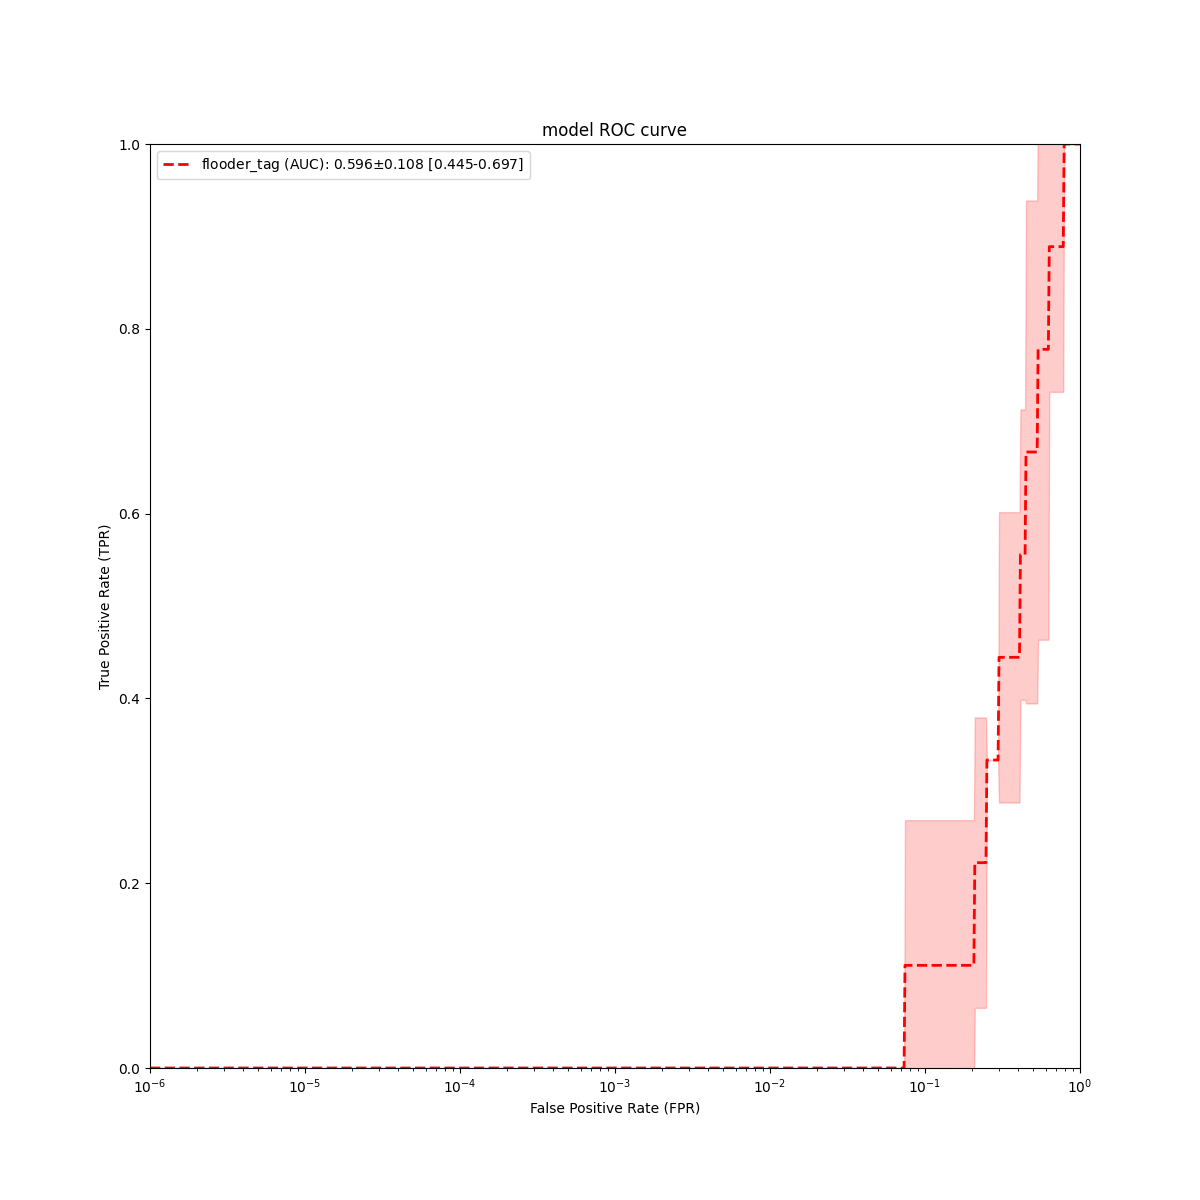
\includegraphics[width=0.8\textwidth]{./results/flooder_tag_roc_aloha.png}
        \vspace*{-1cm}
        \caption{ROC curve and AUC statistics of \textBF{ALOHA} model for the \textbf{Flooder Tag}. The line represents the \textit{mean} TPR at a given FPR, while the shaded region represents the \textit{standard deviation}. Statistics were computed over \textBF{3} training runs, each with random parameter initialization.}
        \label{fig:flooderTagRocAloha}
    \end{figure}
}

\newcommand{\flooderTagRocJointEmbedding}{
    \begin{figure}[H]
        \centering
        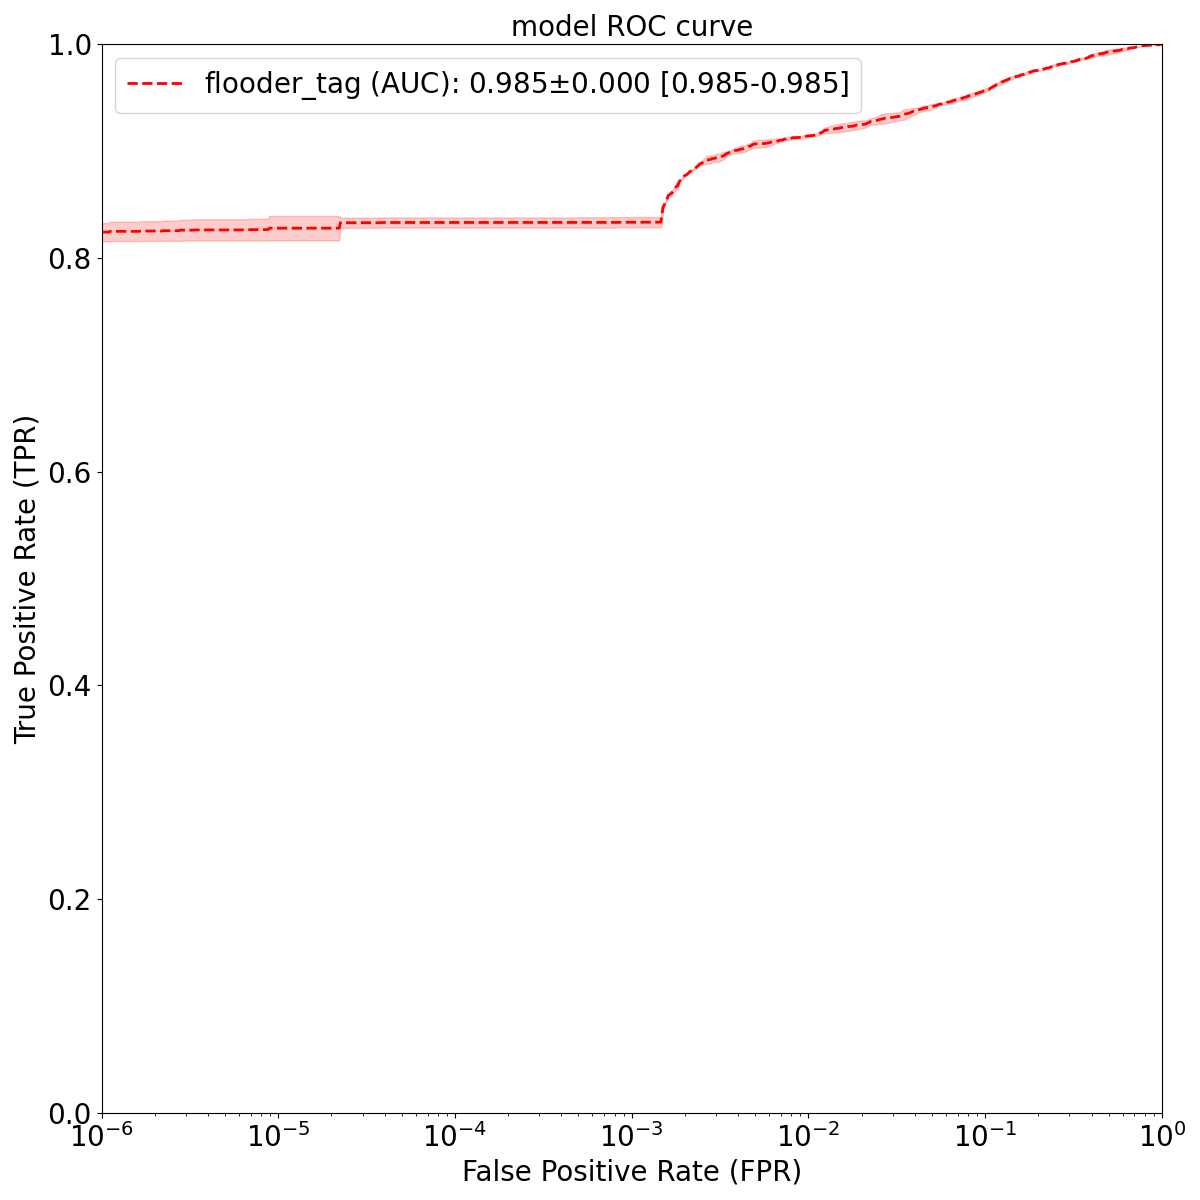
\includegraphics[width=0.8\textwidth]{./results/flooder_tag_roc_jointEmbedding.png}
        \vspace*{-1cm}
        \caption{ROC curve and AUC statistics of \textBF{Joint Embedding} model for the \textbf{Flooder Tag}. The line represents the \textit{mean} TPR at a given FPR, while the shaded region represents the \textit{standard deviation}. Statistics were computed over \textBF{3} training runs, each with random parameter initialization.}
        \label{fig:flooderTagRocJointEmbedding}
    \end{figure}
}

\newcommand{\flooderTagRocProposedMethod}{
    \begin{figure}[H]
        \centering
        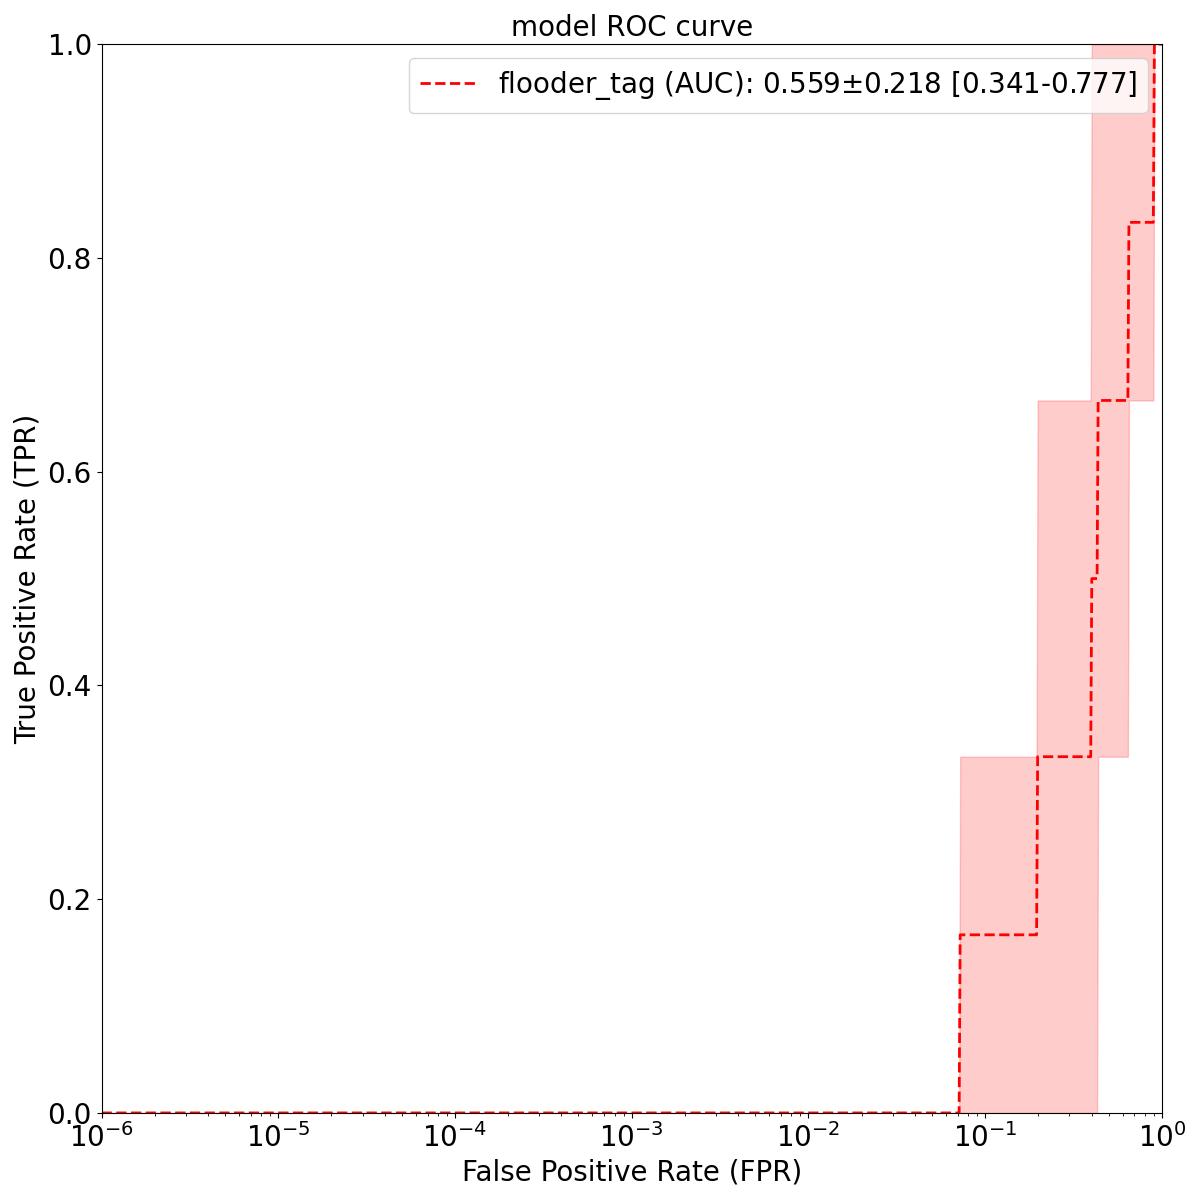
\includegraphics[width=0.8\textwidth]{./results/flooder_tag_roc_proposedModel.png}
        \vspace*{-1cm}
        \caption{ROC curve and AUC statistics of \textBF{Proposed Model} for the \textbf{Flooder Tag}. The line represents the \textit{mean} TPR at a given FPR, while the shaded region represents the \textit{standard deviation}. Statistics were computed over \textBF{3} training runs, each with random parameter initialization.}
        \label{fig:flooderTagRocProposedModel}
    \end{figure}
}

%\newcommand{\installerTagResultsAucTable}{
    \begin{table}[H]
        \centering
        \begin{tabular}{|p{2,8cm}||P{2,4cm} P{2,4cm} P{2,4cm}|}
            \hline
            Installer Tag & ALOHA\newline (M/B only) & ALOHA & Proposed\newline Model \\
            \hline
            AUC-ROC & - & 0.971$\pm$0.004 & \textBF{0.981$\pm$0.000} \\
            \hline
        \end{tabular}
        \caption[Installer Tag prediction task AUC-ROC results]{AUC-ROC (Area Under Curve) of the different models for the \textbf{Installer Tag} prediction task. Results were aggregated over \textBF{2} training runs with different weight initializations and minibatch orderings. Best results are shown in \textbf{bold}.} \label{tab:installerTag_auc}
    \end{table}
}

\newcommand{\installerTagResultsAtFprTable}{
    \begin{center}
        \begin{longtable}[c]{|P{3,2cm}||P{1,8cm} P{1,8cm} P{1,8cm} P{1,8cm} P{1,8cm}|}
            \hline
            Installer Tag & \multicolumn{5}{c|}{{FPR}} \\
            & $10^{-5}$ & $10^{-4}$ & $10^{-3}$ & $10^{-2}$ & $10^{-1}$ \\
            \hline
            \endfirsthead

            \caption*{\raggedright ...continued from previous page} \\
            \hline
            Installer Tag & \multicolumn{5}{c|}{\textbf{FPR}} \\
            & $10^{-5}$ & $10^{-4}$ & $10^{-3}$ & $10^{-2}$ & $10^{-1}$ \\
            \hline
            \endhead

            \caption*{\raggedleft ...continued on next page} \\
            \endfoot

            \caption[Installer Tag prediction task results]{Mean and standard deviation results (TPR, Accuracy, Recall, Precision and F1-Score) of the different models for the \textbf{Installer Tag} prediction task at different \textbf{FPR}s (\textit{False Positive Rates}). Results were aggregated over \textBF{2} training runs with different weight initializations and minibatch orderings. Best results are shown in \textbf{bold}. Under \textbf{TPR} results are also presented the percentage reduction in mean detection error and in ROC curve standard deviation introduced by the \textit{Proposed Model} with respect to both \textit{ALOHA} model and \textit{Joint Embedding}.} \label{tab:installerTag_results_at_fpr} \\
            \endlastfoot

            \multicolumn{6}{|c|}{\textbf{TPR}} \\
            \hline
            ALOHA (M/B only) & - & - & - & - & - \\
            ALOHA & 0.202$\pm$0.004 & 0.288$\pm$0.021 & 0.431$\pm$0.075 & 0.724$\pm$0.044 & 0.908$\pm$0.019 \\
            Proposed Model & 0.220$\pm$0.010 & \textBF{0.340$\pm$0.020} & \textBF{0.515$\pm$0.028} & \textBF{0.773$\pm$0.009} & \textBF{0.951$\pm$0.007} \\
            \hline
            Error Reduction wrt\newline ALOHA (M/B only) & - & - & - & - & - \\
            Error Reduction wrt\newline ALOHA & 2.3\% & 7.3\% & 14.8\% & 17.8\% & 46.7\% \\
            \hline
            Std Reduction wrt\newline ALOHA (M/B only) & - & - & - & - & - \\
            Std Reduction wrt\newline ALOHA & -150.0\% & 4.8\% & 62.7\% & 79.5\% & 63.2\% \\
            \hline
            \multicolumn{6}{|c|}{\textbf{Accuracy}} \\
            \hline
            ALOHA (M/B only) & - & - & - & - & - \\
            ALOHA & 0.986$\pm$0.000 & 0.987$\pm$0.000 & 0.989$\pm$0.001 & 0.985$\pm$0.001 & 0.900$\pm$0.000 \\
            Proposed Model & 0.986$\pm$0.000 & \textBF{0.988$\pm$0.000} & \textBF{0.990$\pm$0.000} & \textBF{0.986$\pm$0.000} & \textBF{0.901$\pm$0.000} \\
            \hline
            \multicolumn{6}{|c|}{\textbf{Recall}} \\
            \hline
            ALOHA (M/B only) & - & - & - & - & - \\
            ALOHA & 0.202$\pm$0.004 & 0.288$\pm$0.021 & 0.431$\pm$0.075 & 0.724$\pm$0.044 & 0.908$\pm$0.019 \\
            Proposed Model & 0.220$\pm$0.010 & \textBF{0.340$\pm$0.020} & \textBF{0.515$\pm$0.028} & \textBF{0.773$\pm$0.009} & \textBF{0.951$\pm$0.007} \\
            \hline
            \multicolumn{6}{|c|}{\textbf{Precision}} \\
            \hline
            ALOHA (M/B only) & - & - & - & - & - \\
            ALOHA & 0.997$\pm$0.000 & 0.981$\pm$0.001 & 0.883$\pm$0.018 & 0.567$\pm$0.015 & 0.141$\pm$0.003 \\
            Proposed Model & \textBF{0.998$\pm$0.000} & \textBF{0.984$\pm$0.001} & \textBF{0.903$\pm$0.004} & \textBF{0.583$\pm$0.003} & \textBF{0.147$\pm$0.001} \\
            \hline
            \multicolumn{6}{|c|}{\textbf{F1 Score}} \\
            \hline
            ALOHA (M/B only) & - & - & - & - & - \\
            ALOHA & 0.337$\pm$0.006 & 0.445$\pm$0.025 & 0.576$\pm$0.072 & 0.636$\pm$0.026 & 0.244$\pm$0.004 \\
            Proposed Model & 0.360$\pm$0.014 & \textBF{0.505$\pm$0.022} & \textBF{0.656$\pm$0.024} & \textBF{0.665$\pm$0.005} & \textBF{0.254$\pm$0.002} \\
            \hline
        \end{longtable}
    \end{center}
}

\newcommand{\installerTagResultsSummaryTable}{
    \begin{table}[H]
        \centering
        \begin{tabular}{|P{3,2cm}||P{1,8cm} P{1,8cm} P{1,8cm} P{1,8cm} P{1,8cm}|}
            \hline
            \multicolumn{6}{|c|}{Installer Tag (at FPR $=1\%$)} \\
            \hline
            Model & TPR & Accuracy & Precision & Recall & F1 score \\
            \hline
            ALOHA (M/B only) & - & - & - & - & - \\
            ALOHA & 0.724$\pm$0.044 & 0.985$\pm$0.001 & 0.567$\pm$0.015 & 0.724$\pm$0.044 & 0.636$\pm$0.026 \\
            Proposed Model & \textBF{0.773$\pm$0.009} & \textBF{0.986$\pm$0.000} & \textBF{0.583$\pm$0.003} & \textBF{0.773$\pm$0.009} & \textBF{0.665$\pm$0.005} \\
            \hline
        \end{tabular}
        \caption[Summary of Installer Tag prediction task results]{Summary of the mean and standard deviation results of the different models for the \textbf{Installer Tag} prediction task at \textbf{FPR} $=1\%$. Results were aggregated over \textBF{2} training runs with different weight initializations and minibatch orderings. Best results are shown in \textbf{bold}.} \label{tab:installerTag_result_summary}
    \end{table}
}

\newcommand{\installerTagRocAlohaMB}{
    \begin{figure}[H]
        \vspace*{-0.5cm}
        \centering
        \includegraphics[width=0.6\textwidth]{./results/installer_tag_roc_alohaMB.png}
        \vspace*{-0.2cm}
        \caption[Installer Tag prediction task ALOHA (M/B only) ROC curve]{ROC curve and AUC statistics of \textBF{ALOHA (M/B only)} model for the \textbf{Installer Tag}. The line represents the \textit{mean} TPR at a given FPR, while the shaded region represents the \textit{standard deviation}. Statistics were computed over \textBF{2} training runs, each with random parameter initialization.}
        \label{fig:installerTagRocAlohaMB}
    \end{figure}
}

\newcommand{\installerTagRocAloha}{
    \begin{figure}[H]
        \vspace*{-0.5cm}
        \centering
        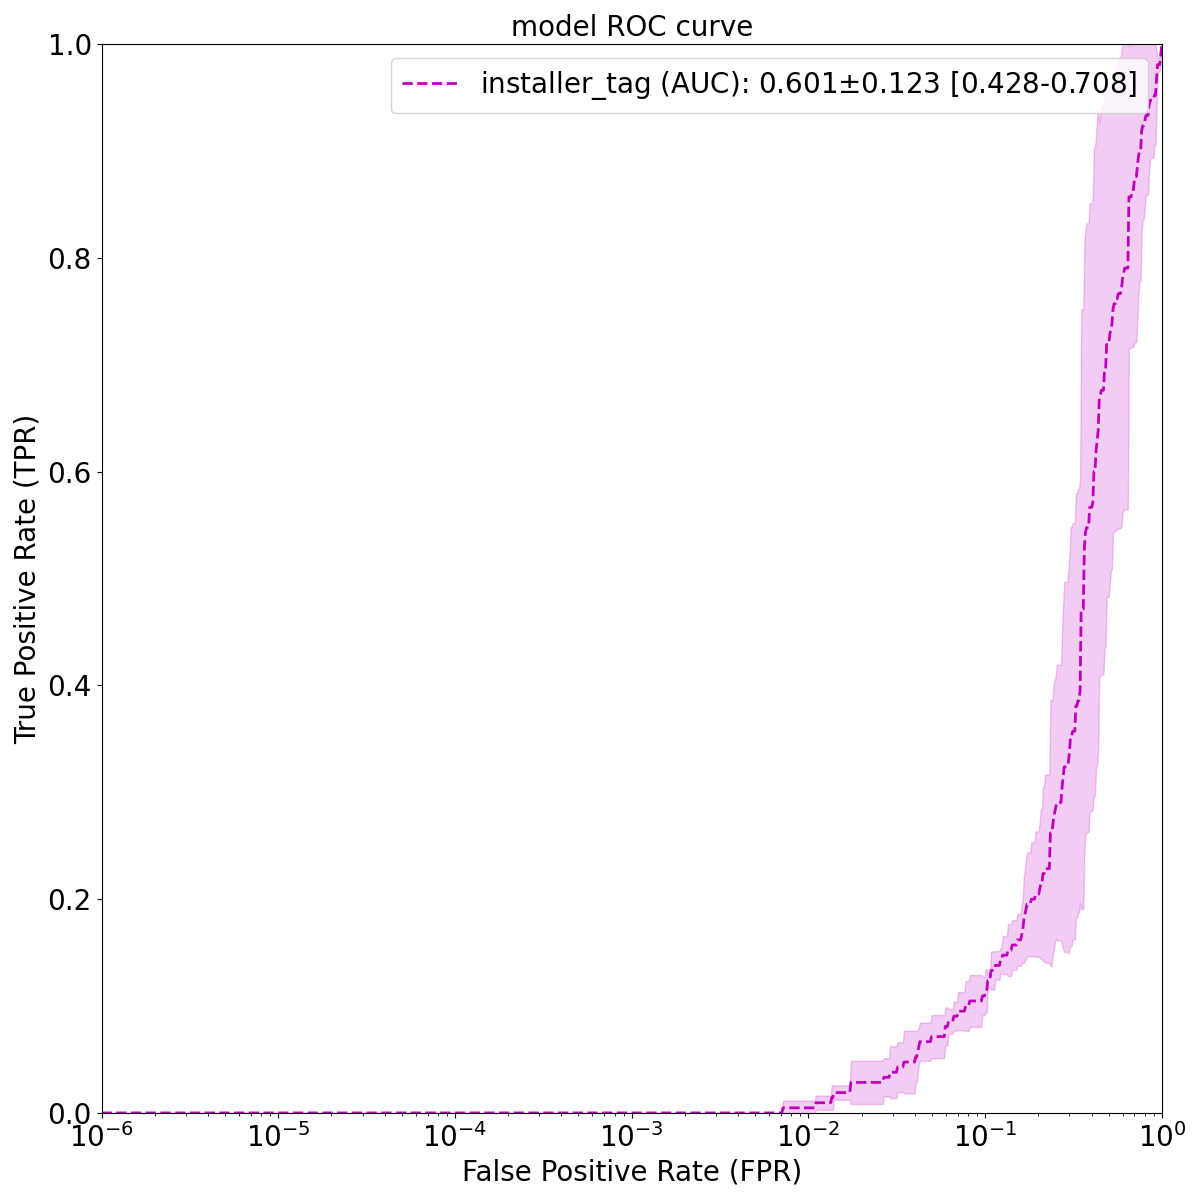
\includegraphics[width=0.6\textwidth]{./results/installer_tag_roc_aloha.png}
        \vspace*{-0.2cm}
        \caption[Installer Tag prediction task ALOHA ROC curve]{ROC curve and AUC statistics of \textBF{ALOHA} model for the \textbf{Installer Tag}. The line represents the \textit{mean} TPR at a given FPR, while the shaded region represents the \textit{standard deviation}. Statistics were computed over \textBF{2} training runs, each with random parameter initialization.}
        \label{fig:installerTagRocAloha}
    \end{figure}
}

\newcommand{\installerTagRocProposedMethod}{
    \begin{figure}[H]
        \vspace*{-0.5cm}
        \centering
        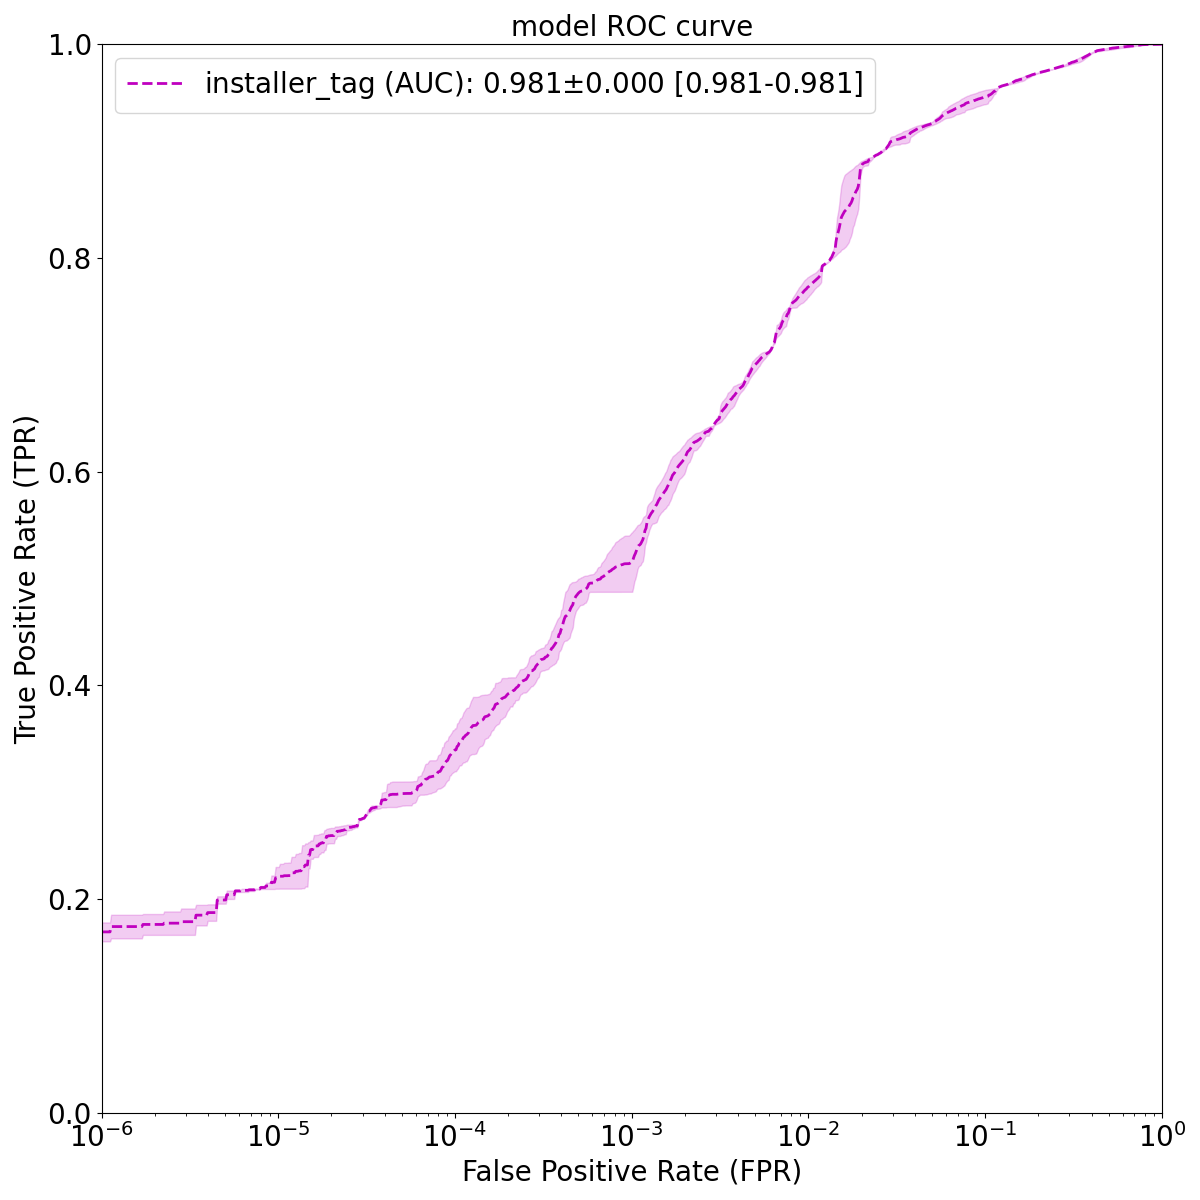
\includegraphics[width=0.6\textwidth]{./results/installer_tag_roc_proposedModel.png}
        \vspace*{-0.2cm}
        \caption[Installer Tag prediction task Proposed Model ROC curve]{ROC curve and AUC statistics of \textBF{Proposed Model} for the \textbf{Installer Tag}. The line represents the \textit{mean} TPR at a given FPR, while the shaded region represents the \textit{standard deviation}. Statistics were computed over \textBF{2} training runs, each with random parameter initialization.}
        \label{fig:installerTagRocProposedModel}
    \end{figure}
}

%\newcommand{\packedTagResultsAucTable}{
    \begin{table}[h!]
        \centering
        \begin{tabular}{|p{2,8cm}||P{2,2cm} P{2,2cm} P{2,2cm} P{2,2cm}|}
            \hline
            Packed Tag & ALOHA\newline (M/B only) & ALOHA & Joint\newline Embedding & Proposed\newline Model \\
            \hline
            AUC-ROC & - & 0.978$\pm$0.001 & 0.978$\pm$0.003 & \textBF{0.983$\pm$0.002} \\
            \hline
        \end{tabular}
        \caption[Packed Tag prediction task AUC-ROC results]{AUC-ROC (Area Under Curve) of the different models for the \textbf{Packed Tag} prediction task. Results were aggregated over \textBF{3} training runs with different weight initializations and minibatch orderings. Best results are shown in \textbf{bold}.} \label{tab:packedTag_auc}
    \end{table}
}

\newcommand{\packedTagResultsAtFprTable}{
    \begin{center}
        \begin{longtable}[c]{|P{3,2cm}||P{1,8cm} P{1,8cm} P{1,8cm} P{1,8cm} P{1,8cm}|}
            \hline
            Packed Tag & \multicolumn{5}{c|}{{FPR}} \\
            & $10^{-5}$ & $10^{-4}$ & $10^{-3}$ & $10^{-2}$ & $10^{-1}$ \\
            \hline
            \endfirsthead

            \caption*{\raggedright ...continued from previous page} \\
            \hline
            Packed Tag & \multicolumn{5}{c|}{\textbf{FPR}} \\
            & $10^{-5}$ & $10^{-4}$ & $10^{-3}$ & $10^{-2}$ & $10^{-1}$ \\
            \hline
            \endhead

            \caption*{\raggedleft ...continued on next page} \\
            \endfoot

            \caption[Packed Tag prediction task results]{Mean and standard deviation results (TPR, Accuracy, Recall, Precision and F1-Score) of the different models for the \textbf{Packed Tag} prediction task at different \textbf{FPR}s (\textit{False Positive Rates}). Results were aggregated over \textBF{3} training runs with different weight initializations and minibatch orderings. Best results are shown in \textbf{bold}. Under \textbf{TPR} results are also presented the percentage reduction in mean detection error and in ROC curve standard deviation introduced by the \textit{Proposed Model} with respect to both \textit{ALOHA} model and \textit{Joint Embedding}.} \label{tab:packedTag_results_at_fpr} \\
            \endlastfoot

            \multicolumn{6}{|c|}{\textbf{TPR}} \\
            \hline
            ALOHA (M/B only) & - & - & - & - & - \\
            ALOHA & 0.011$\pm$0.013 & 0.223$\pm$0.134 & 0.593$\pm$0.013 & 0.675$\pm$0.017 & 0.945$\pm$0.005 \\
            Joint Embedding & 0.003$\pm$0.003 & 0.224$\pm$0.057 & 0.611$\pm$0.016 & 0.731$\pm$0.019 & 0.939$\pm$0.010 \\
            Proposed Model & \textBF{0.080$\pm$0.031} & \textBF{0.325$\pm$0.082} & \textBF{0.628$\pm$0.012} & \textBF{0.758$\pm$0.016} & \textBF{0.946$\pm$0.015} \\
            \hline
            Error Reduction wrt\newline ALOHA (M/B only) & - & - & - & - & - \\
            Error Reduction wrt\newline ALOHA & 7.0\% & 13.1\% & 8.6\% & 25.5\% & 1.8\% \\
            Error Reduction wrt\newline Joint Embedding & 7.7\% & 13.0\% & 4.4\% & 10.0\% & 11.5\% \\
            \hline
            Std Reduction wrt\newline ALOHA (M/B only) & - & - & - & - & - \\
            Std Reduction wrt\newline ALOHA & -138.5\% & 38.8\% & 7.7\% & 5.9\% & -200.0\% \\
            Std Reduction wrt\newline Joint Embedding & -933.3\% & -43.9\% & 25.0\% & 15.8\% & -50.0\% \\
            \hline
            \multicolumn{6}{|c|}{\textbf{Accuracy}} \\
            \hline
            ALOHA (M/B only) & - & - & - & - & - \\
            ALOHA & 0.865$\pm$0.002 & 0.894$\pm$0.018 & 0.944$\pm$0.002 & 0.947$\pm$0.002 & \textBF{0.906$\pm$0.001} \\
            Joint Embedding & 0.864$\pm$0.000 & 0.894$\pm$0.008 & 0.946$\pm$0.002 & 0.955$\pm$0.003 & 0.905$\pm$0.001 \\
            Proposed Model & \textBF{0.874$\pm$0.004} & \textBF{0.908$\pm$0.011} & \textBF{0.948$\pm$0.002} & \textBF{0.958$\pm$0.002} & 0.906$\pm$0.002 \\
            \hline
            \multicolumn{6}{|c|}{\textbf{Recall}} \\
            \hline
            ALOHA (M/B only) & - & - & - & - & - \\
            ALOHA & 0.011$\pm$0.013 & 0.223$\pm$0.134 & 0.593$\pm$0.013 & 0.675$\pm$0.017 & 0.945$\pm$0.005 \\
            Joint Embedding & 0.003$\pm$0.003 & 0.224$\pm$0.057 & 0.611$\pm$0.016 & 0.731$\pm$0.019 & 0.939$\pm$0.010 \\
            Proposed Model & \textBF{0.080$\pm$0.031} & \textBF{0.325$\pm$0.082} & \textBF{0.628$\pm$0.012} & \textBF{0.758$\pm$0.016} & \textBF{0.946$\pm$0.015} \\
            \hline
            \multicolumn{6}{|c|}{\textbf{Precision}} \\
            \hline
            ALOHA (M/B only) & - & - & - & - & - \\
            ALOHA & 0.986$\pm$0.013 & 0.992$\pm$0.008 & 0.989$\pm$0.000 & 0.914$\pm$0.002 & \textBF{0.599$\pm$0.001} \\
            Joint Embedding & 0.998$\pm$0.002 & 0.997$\pm$0.001 & \textBF{0.990$\pm$0.000} & 0.920$\pm$0.002 & 0.598$\pm$0.003 \\
            Proposed Model & \textBF{0.999$\pm$0.000} & \textBF{0.998$\pm$0.000} & \textBF{0.990$\pm$0.000} & \textBF{0.923$\pm$0.002} & 0.599$\pm$0.004 \\
            \hline
            \multicolumn{6}{|c|}{\textbf{F1 Score}} \\
            \hline
            ALOHA (M/B only) & - & - & - & - & - \\
            ALOHA & 0.022$\pm$0.025 & 0.343$\pm$0.197 & 0.741$\pm$0.010 & 0.776$\pm$0.012 & 0.733$\pm$0.003 \\
            Joint Embedding & 0.005$\pm$0.006 & 0.362$\pm$0.073 & 0.756$\pm$0.012 & 0.815$\pm$0.012 & 0.730$\pm$0.005 \\
            Proposed Model & \textBF{0.146$\pm$0.052} & \textBF{0.484$\pm$0.093} & \textBF{0.769$\pm$0.009} & \textBF{0.832$\pm$0.010} & \textBF{0.734$\pm$0.007} \\
            \hline
        \end{longtable}
    \end{center}
}

\newcommand{\packedTagResultsSummaryTable}{
    \begin{table}[h!]
        \centering
        \begin{tabular}{|P{3,2cm}||P{1,8cm} P{1,8cm} P{1,8cm} P{1,8cm} P{1,8cm}|}
            \hline
            \multicolumn{6}{|c|}{Packed Tag (at FPR $=1\%$)} \\
            \hline
            Model & TPR & Accuracy & Precision & Recall & F1 score \\
            \hline
            ALOHA (M/B only) & - & - & - & - & - \\
            ALOHA & 0.675$\pm$0.017 & 0.947$\pm$0.002 & 0.914$\pm$0.002 & 0.675$\pm$0.017 & 0.776$\pm$0.012 \\
            Joint Embedding & 0.731$\pm$0.019 & 0.955$\pm$0.003 & 0.920$\pm$0.002 & 0.731$\pm$0.019 & 0.815$\pm$0.012 \\
            Proposed Model & \textBF{0.758$\pm$0.016} & \textBF{0.958$\pm$0.002} & \textBF{0.923$\pm$0.002} & \textBF{0.758$\pm$0.016} & \textBF{0.832$\pm$0.010} \\
            \hline
        \end{tabular}
        \caption[Summary of Packed Tag prediction task results]{Summary of the mean and standard deviation results of the different models for the \textbf{Packed Tag} prediction task at \textbf{FPR} $=1\%$. Results were aggregated over \textBF{3} training runs with different weight initializations and minibatch orderings. Best results are shown in \textbf{bold}.} \label{tab:packedTag_result_summary}
    \end{table}
}

\newcommand{\packedTagRocAlohaMB}{
    \begin{figure}[h!]
        \vspace*{-0.5cm}
        \centering
        \includegraphics[width=0.6\textwidth]{./results/packed_tag_roc_alohaMB.png}
        \vspace*{-0.2cm}
        \caption[Packed Tag prediction task ALOHA (M/B only) ROC curve]{ROC curve and AUC statistics of \textBF{ALOHA (M/B only)} model for the \textbf{Packed Tag}. The line represents the \textit{mean} TPR at a given FPR, while the shaded region represents the \textit{standard deviation}. Statistics were computed over \textBF{3} training runs, each with random parameter initialization.}
        \label{fig:packedTagRocAlohaMB}
    \end{figure}
}

\newcommand{\packedTagRocAloha}{
    \begin{figure}[h!]
        \vspace*{-0.5cm}
        \centering
        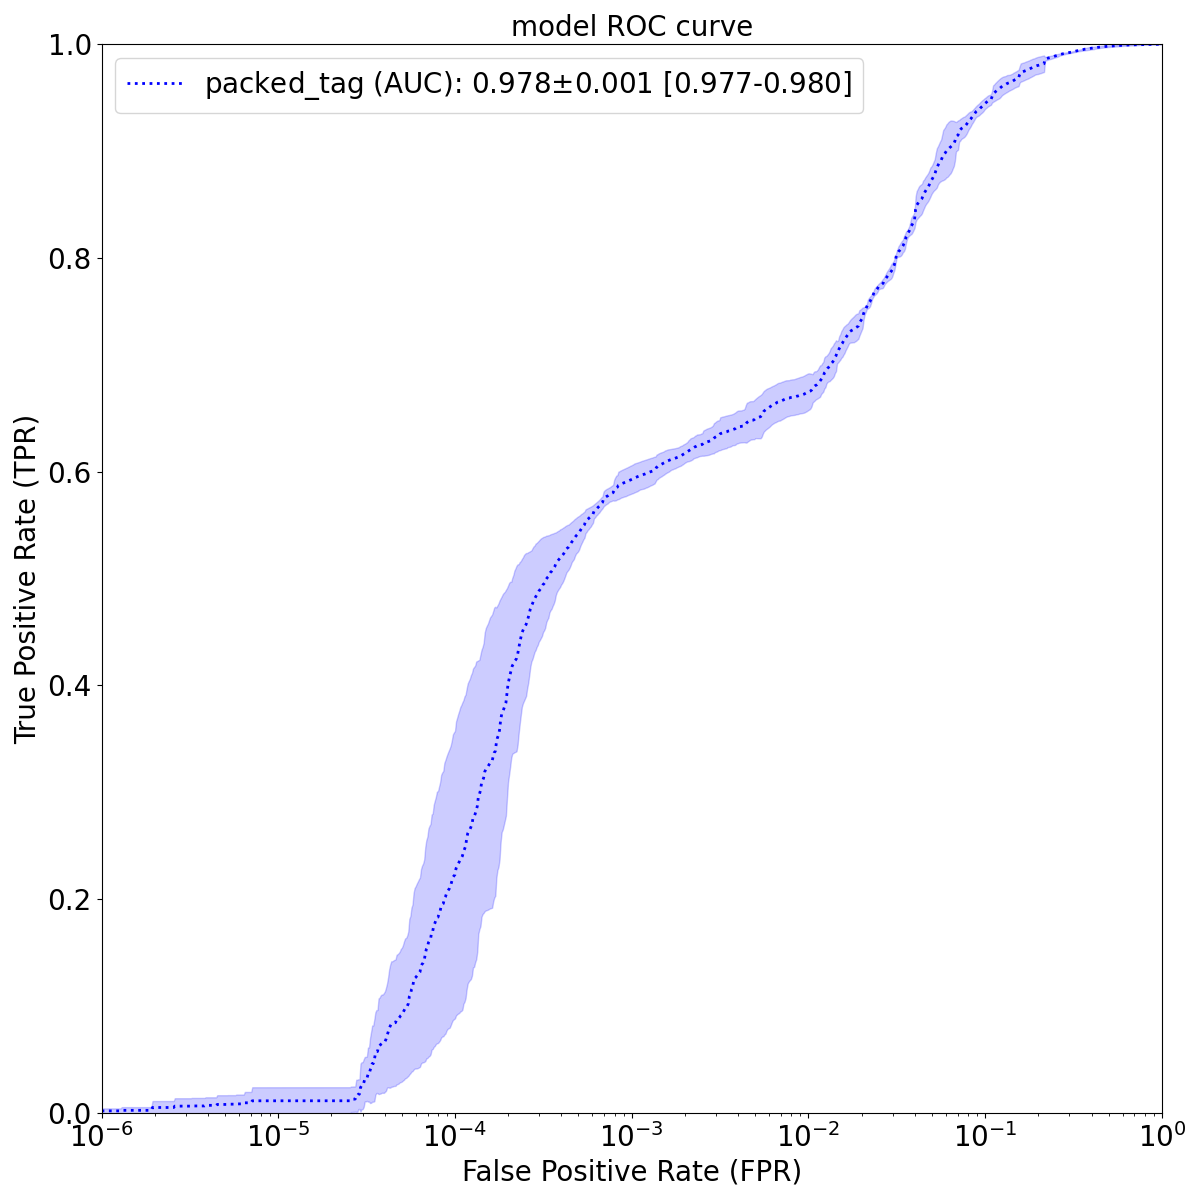
\includegraphics[width=0.6\textwidth]{./results/packed_tag_roc_aloha.png}
        \vspace*{-0.2cm}
        \caption[Packed Tag prediction task ALOHA ROC curve]{ROC curve and AUC statistics of \textBF{ALOHA} model for the \textbf{Packed Tag}. The line represents the \textit{mean} TPR at a given FPR, while the shaded region represents the \textit{standard deviation}. Statistics were computed over \textBF{3} training runs, each with random parameter initialization.}
        \label{fig:packedTagRocAloha}
    \end{figure}
}

\newcommand{\packedTagRocJointEmbedding}{
    \begin{figure}[h!]
        \vspace*{-0.5cm}
        \centering
        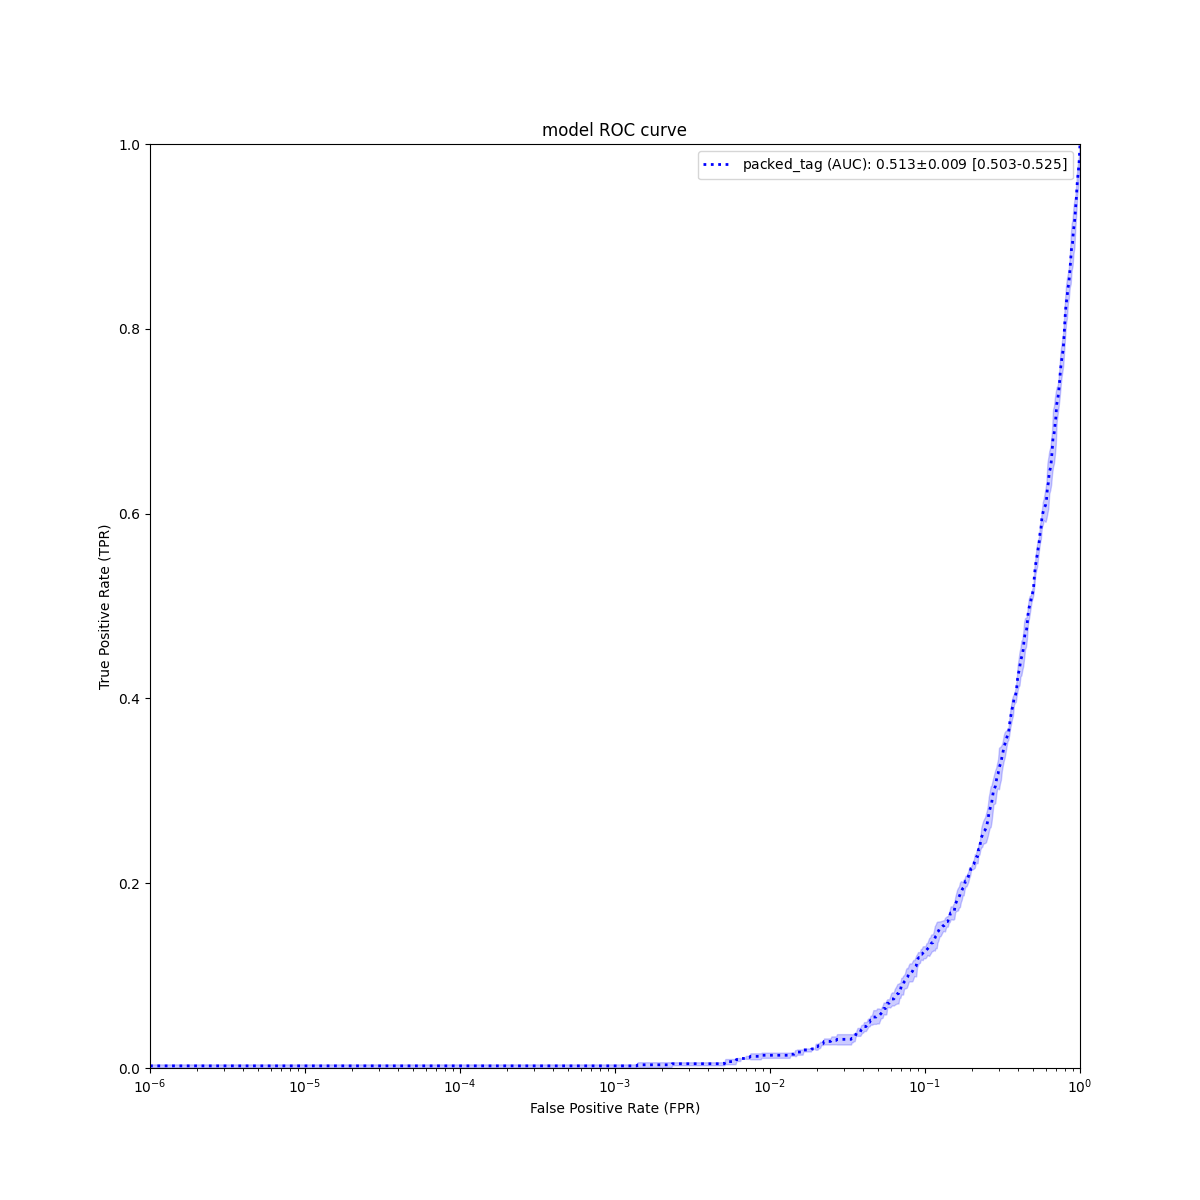
\includegraphics[width=0.6\textwidth]{./results/packed_tag_roc_jointEmbedding.png}
        \vspace*{-0.2cm}
        \caption[Packed Tag prediction task Joint Embedding ROC curve]{ROC curve and AUC statistics of \textBF{Joint Embedding} model for the \textbf{Packed Tag}. The line represents the \textit{mean} TPR at a given FPR, while the shaded region represents the \textit{standard deviation}. Statistics were computed over \textBF{3} training runs, each with random parameter initialization.}
        \label{fig:packedTagRocJointEmbedding}
    \end{figure}
}

\newcommand{\packedTagRocProposedMethod}{
    \begin{figure}[h!]
        \vspace*{-0.5cm}
        \centering
        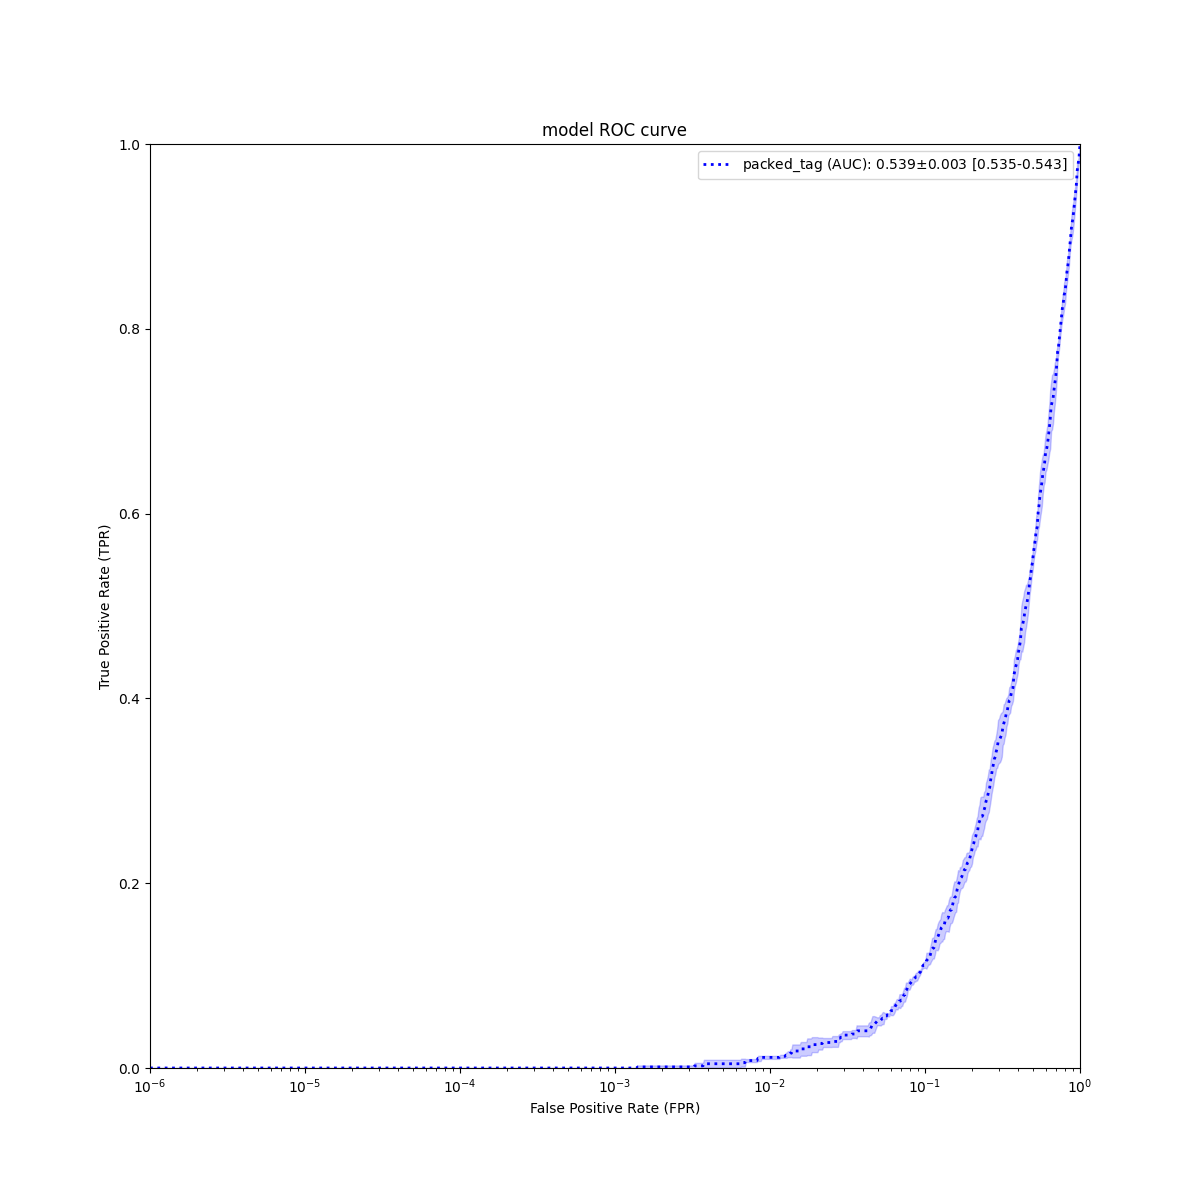
\includegraphics[width=0.6\textwidth]{./results/packed_tag_roc_proposedModel.png}
        \vspace*{-0.2cm}
        \caption[Packed Tag prediction task Proposed Model ROC curve]{ROC curve and AUC statistics of \textBF{Proposed Model} for the \textbf{Packed Tag}. The line represents the \textit{mean} TPR at a given FPR, while the shaded region represents the \textit{standard deviation}. Statistics were computed over \textBF{3} training runs, each with random parameter initialization.}
        \label{fig:packedTagRocProposedModel}
    \end{figure}
}

%\newcommand{\ransomwareTagResultsAucTable}{
    \begin{table}[H]
        \centering
        \begin{tabular}{|p{2,8cm}||P{2,2cm} P{2,2cm} P{2,2cm} P{2,2cm}|}
            \hline
            Ransomware Tag & ALOHA\newline (M/B only) & ALOHA & Joint\newline Embedding & Proposed\newline Model \\
            \hline
            AUC-ROC & - & 0.979$\pm$0.003 & 0.979$\pm$0.004 & \textBF{0.984$\pm$0.005} \\
            \hline
        \end{tabular}
        \caption{AUC-ROC (Area Under Curve) of the different models for the \textbf{Ransomware Tag} prediction task. Results were aggregated over \textBF{3} training runs with different weight initializations and minibatch orderings. Best results are shown in \textbf{bold}.} \label{tab:ransomwareTag_auc}
    \end{table}
}

\newcommand{\ransomwareTagResultsAtFprTable}{
    \begin{center}
        \begin{longtable}[c]{|P{3,2cm}||P{1,8cm} P{1,8cm} P{1,8cm} P{1,8cm} P{1,8cm}|}
            \hline
            Ransomware Tag & \multicolumn{5}{c|}{{FPR}} \\
            & $10^{-5}$ & $10^{-4}$ & $10^{-3}$ & $10^{-2}$ & $10^{-1}$ \\
            \hline
            \endfirsthead

            \caption*{\raggedright ...continued from previous page} \\
            \hline
            Ransomware Tag & \multicolumn{5}{c|}{\textbf{FPR}} \\
            & $10^{-5}$ & $10^{-4}$ & $10^{-3}$ & $10^{-2}$ & $10^{-1}$ \\
            \hline
            \endhead

            \caption*{\raggedleft ...continued on next page} \\
            \endfoot

            \caption{Mean and standard deviation results (TPR, Accuracy, Recall, Precision and F1-Score) of the different models for the \textbf{Ransomware Tag} prediction task at different \textbf{FPR}s (\textit{False Positive Rates}). Results were aggregated over \textBF{3} training runs with different weight initializations and minibatch orderings. Best results are shown in \textbf{bold}. Under \textbf{TPR} results are also presented the percentage reduction in mean detection error and in ROC curve standard deviation introduced by the \textit{Proposed Model} with respect to both \textit{ALOHA} model and \textit{Joint Embedding}.} \label{tab:ransomwareTag_results_at_fpr} \\
            \endlastfoot

            \multicolumn{6}{|c|}{\textbf{TPR}} \\
            \hline
            ALOHA (M/B only) & - & - & - & - & - \\
            ALOHA & 0.808$\pm$0.030 & 0.831$\pm$0.010 & 0.843$\pm$0.001 & 0.849$\pm$0.001 & 0.914$\pm$0.015 \\
            Joint Embedding & \textBF{0.825$\pm$0.008} & \textBF{0.842$\pm$0.001} & 0.849$\pm$0.001 & 0.855$\pm$0.002 & 0.927$\pm$0.014 \\
            Proposed Model & 0.818$\pm$0.012 & 0.840$\pm$0.002 & \textBF{0.850$\pm$0.001} & \textBF{0.858$\pm$0.003} & \textBF{0.944$\pm$0.024} \\
            \hline
            Error Reduction wrt\newline ALOHA (M/B only) & - & - & - & - & - \\
            Error Reduction wrt\newline ALOHA & 5.2\% & 5.3\% & 4.5\% & 6.0\% & 34.9\% \\
            Error Reduction wrt\newline Joint Embedding & -4.0\% & -1.3\% & 0.7\% & 2.1\% & 23.3\% \\
            \hline
            Std Reduction wrt\newline ALOHA (M/B only) & - & - & - & - & - \\
            Std Reduction wrt\newline ALOHA & 60.0\% & 80.0\% & 0.0\% & -200.0\% & -60.0\% \\
            Std Reduction wrt\newline Joint Embedding & -50.0\% & -100.0\% & 0.0\% & -50.0\% & -71.4\% \\
            \hline
            \multicolumn{6}{|c|}{\textbf{Accuracy}} \\
            \hline
            ALOHA (M/B only) & - & - & - & - & - \\
            ALOHA & 0.990$\pm$0.002 & 0.991$\pm$0.001 & \textBF{0.991$\pm$0.000} & \textBF{0.983$\pm$0.000} & 0.901$\pm$0.001 \\
            Joint Embedding & \textBF{0.991$\pm$0.000} & \textBF{0.992$\pm$0.000} & \textBF{0.991$\pm$0.000} & \textBF{0.983$\pm$0.000} & 0.901$\pm$0.001 \\
            Proposed Model & 0.990$\pm$0.001 & \textBF{0.992$\pm$0.000} & \textBF{0.991$\pm$0.000} & \textBF{0.983$\pm$0.000} & \textBF{0.902$\pm$0.001} \\
            \hline
            \multicolumn{6}{|c|}{\textbf{Recall}} \\
            \hline
            ALOHA (M/B only) & - & - & - & - & - \\
            ALOHA & 0.808$\pm$0.030 & 0.831$\pm$0.010 & 0.843$\pm$0.001 & 0.849$\pm$0.001 & 0.914$\pm$0.015 \\
            Joint Embedding & \textBF{0.825$\pm$0.008} & \textBF{0.842$\pm$0.001} & 0.849$\pm$0.001 & 0.855$\pm$0.002 & 0.927$\pm$0.014 \\
            Proposed Model & 0.818$\pm$0.012 & 0.840$\pm$0.002 & \textBF{0.850$\pm$0.001} & \textBF{0.858$\pm$0.003} & \textBF{0.944$\pm$0.024} \\
            \hline
            \multicolumn{6}{|c|}{\textbf{Precision}} \\
            \hline
            ALOHA (M/B only) & - & - & - & - & - \\
            ALOHA & \textBF{1.000$\pm$0.000} & \textBF{0.998$\pm$0.000} & 0.979$\pm$0.000 & 0.824$\pm$0.000 & 0.335$\pm$0.004 \\
            Joint Embedding & \textBF{1.000$\pm$0.000} & \textBF{0.998$\pm$0.000} & 0.979$\pm$0.000 & 0.825$\pm$0.000 & 0.338$\pm$0.003 \\
            Proposed Model & \textBF{1.000$\pm$0.000} & \textBF{0.998$\pm$0.000} & \textBF{0.980$\pm$0.001} & \textBF{0.826$\pm$0.001} & \textBF{0.343$\pm$0.006} \\
            \hline
            \multicolumn{6}{|c|}{\textbf{F1 Score}} \\
            \hline
            ALOHA (M/B only) & - & - & - & - & - \\
            ALOHA & 0.894$\pm$0.019 & 0.907$\pm$0.006 & 0.906$\pm$0.001 & 0.836$\pm$0.001 & 0.491$\pm$0.006 \\
            Joint Embedding & \textBF{0.904$\pm$0.005} & \textBF{0.913$\pm$0.001} & 0.909$\pm$0.000 & 0.840$\pm$0.001 & 0.496$\pm$0.006 \\
            Proposed Model & 0.900$\pm$0.007 & 0.912$\pm$0.001 & \textBF{0.910$\pm$0.000} & \textBF{0.841$\pm$0.002} & \textBF{0.503$\pm$0.010} \\
            \hline
        \end{longtable}
    \end{center}
}

\newcommand{\ransomwareTagResultsSummaryTable}{
    \begin{table}[H]
        \centering
        \begin{tabular}{|P{3,2cm}||P{1,8cm} P{1,8cm} P{1,8cm} P{1,8cm} P{1,8cm}|}
            \hline
            \multicolumn{6}{|c|}{Ransomware Tag (at FPR $=1\%$)} \\
            \hline
            Model & TPR & Accuracy & Precision & Recall & F1 score \\
            \hline
            ALOHA (M/B only) & - & - & - & - & - \\
            ALOHA & 0.849$\pm$0.001 & \textBF{0.983$\pm$0.000} & 0.824$\pm$0.000 & 0.849$\pm$0.001 & 0.836$\pm$0.001 \\
            Joint Embedding & 0.855$\pm$0.002 & \textBF{0.983$\pm$0.000} & 0.825$\pm$0.000 & 0.855$\pm$0.002 & 0.840$\pm$0.001 \\
            Proposed Model & \textBF{0.858$\pm$0.003} & \textBF{0.983$\pm$0.000} & \textBF{0.826$\pm$0.001} & \textBF{0.858$\pm$0.003} & \textBF{0.841$\pm$0.002} \\
            \hline
        \end{tabular}
        \caption{Summary of the mean and standard deviation results of the different models for the \textbf{Ransomware Tag} prediction task at \textbf{FPR} $=1\%$. Results were aggregated over \textBF{3} training runs with different weight initializations and minibatch orderings. Best results are shown in \textbf{bold}.} \label{tab:ransomwareTag_result_summary}
    \end{table}
}

\newcommand{\ransomwareTagRocAlohaMB}{
    \begin{figure}[H]
        \vspace*{-0.5cm}
        \centering
        \includegraphics[width=0.6\textwidth]{./results/ransomware_tag_roc_alohaMB.png}
        \vspace*{-0.2cm}
        \caption{ROC curve and AUC statistics of \textBF{ALOHA (M/B only)} model for the \textbf{Ransomware Tag}. The line represents the \textit{mean} TPR at a given FPR, while the shaded region represents the \textit{standard deviation}. Statistics were computed over \textBF{3} training runs, each with random parameter initialization.}
        \label{fig:ransomwareTagRocAlohaMB}
    \end{figure}
}

\newcommand{\ransomwareTagRocAloha}{
    \begin{figure}[H]
        \vspace*{-0.5cm}
        \centering
        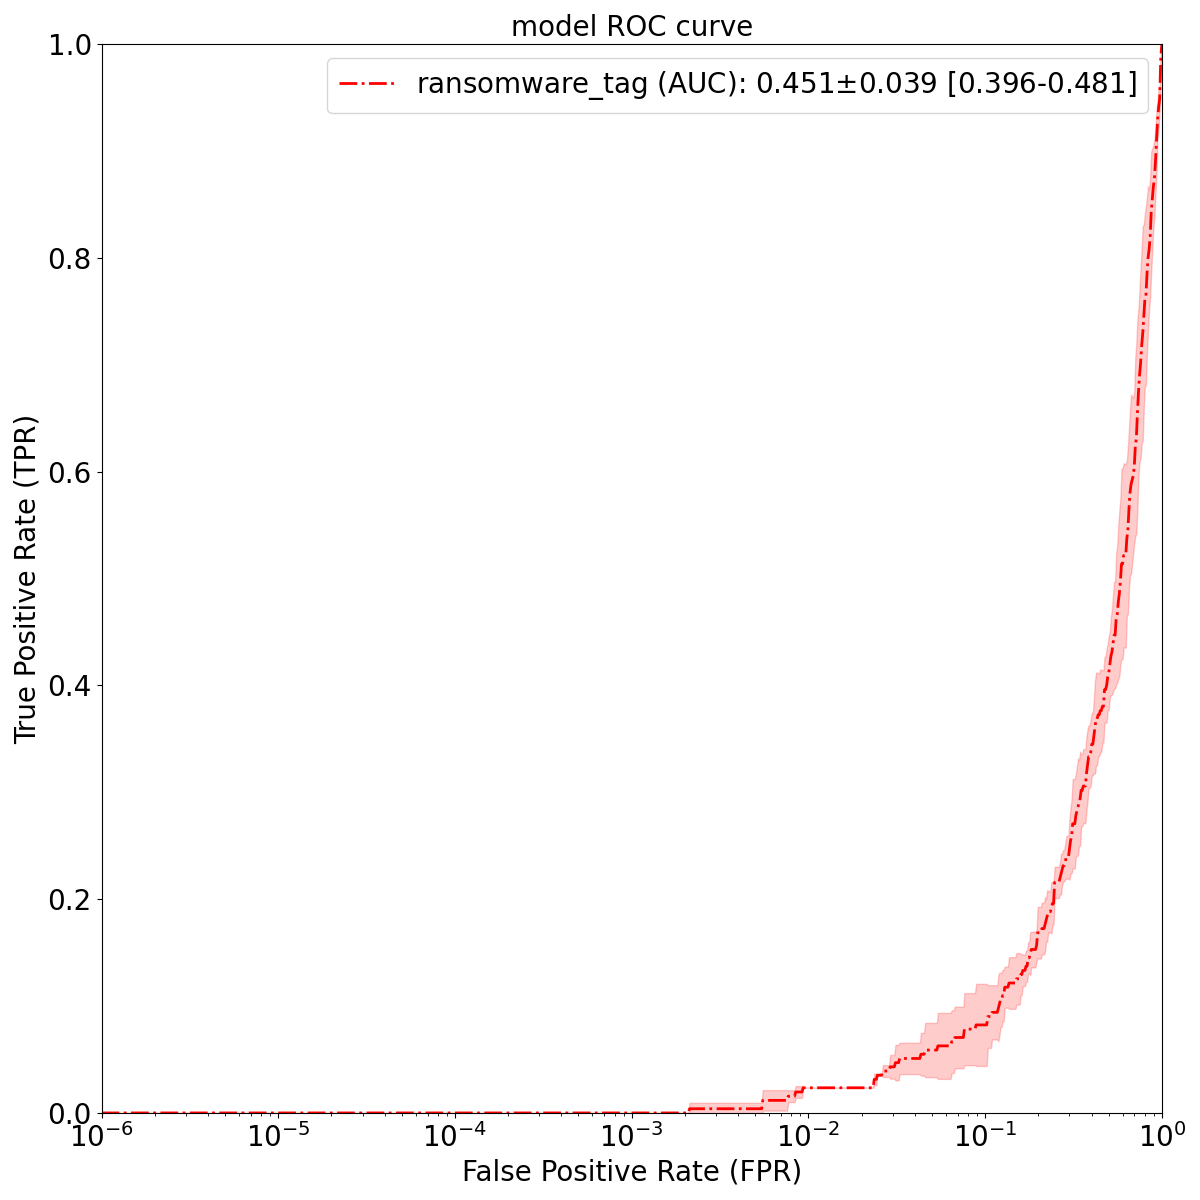
\includegraphics[width=0.6\textwidth]{./results/ransomware_tag_roc_aloha.png}
        \vspace*{-0.2cm}
        \caption{ROC curve and AUC statistics of \textBF{ALOHA} model for the \textbf{Ransomware Tag}. The line represents the \textit{mean} TPR at a given FPR, while the shaded region represents the \textit{standard deviation}. Statistics were computed over \textBF{3} training runs, each with random parameter initialization.}
        \label{fig:ransomwareTagRocAloha}
    \end{figure}
}

\newcommand{\ransomwareTagRocJointEmbedding}{
    \begin{figure}[H]
        \vspace*{-0.5cm}
        \centering
        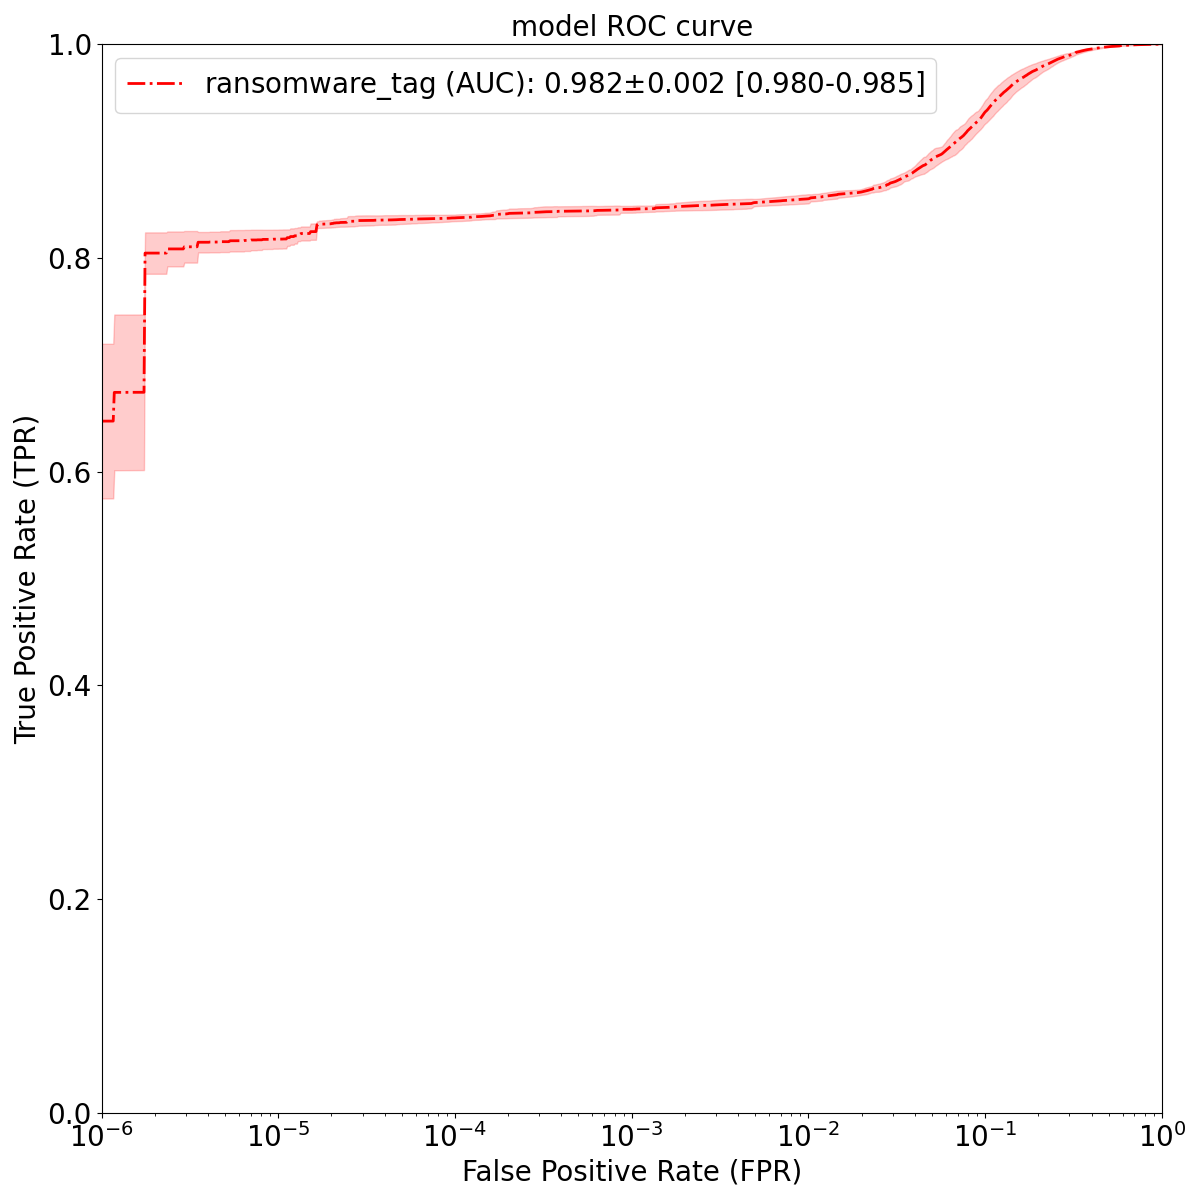
\includegraphics[width=0.6\textwidth]{./results/ransomware_tag_roc_jointEmbedding.png}
        \vspace*{-0.2cm}
        \caption{ROC curve and AUC statistics of \textBF{Joint Embedding} model for the \textbf{Ransomware Tag}. The line represents the \textit{mean} TPR at a given FPR, while the shaded region represents the \textit{standard deviation}. Statistics were computed over \textBF{3} training runs, each with random parameter initialization.}
        \label{fig:ransomwareTagRocJointEmbedding}
    \end{figure}
}

\newcommand{\ransomwareTagRocProposedMethod}{
    \begin{figure}[H]
        \vspace*{-0.5cm}
        \centering
        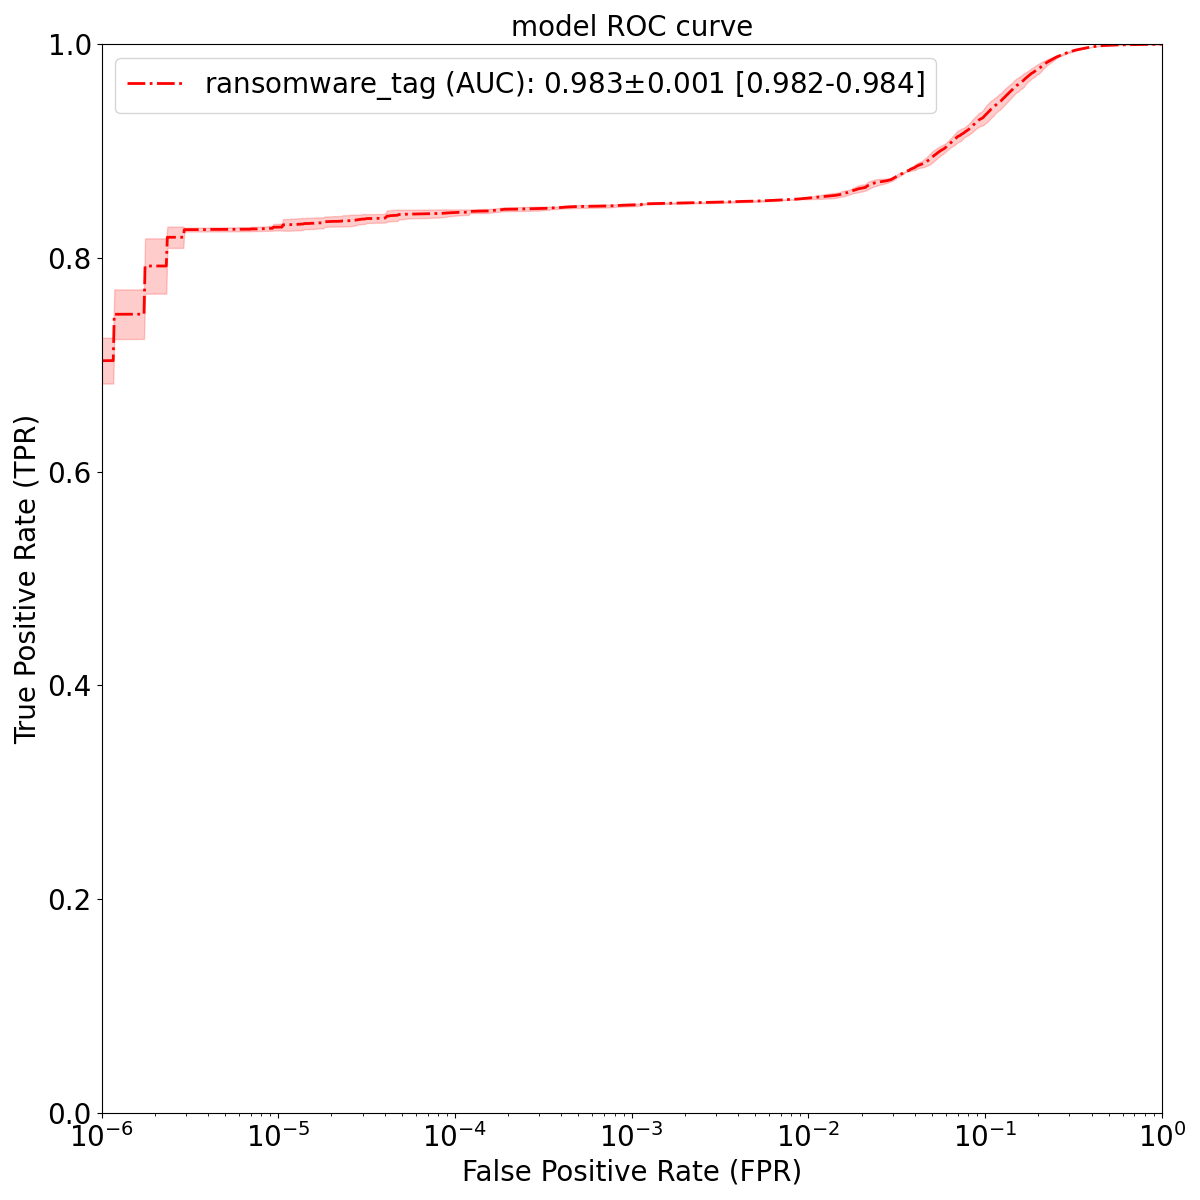
\includegraphics[width=0.6\textwidth]{./results/ransomware_tag_roc_proposedModel.png}
        \vspace*{-0.2cm}
        \caption{ROC curve and AUC statistics of \textBF{Proposed Model} for the \textbf{Ransomware Tag}. The line represents the \textit{mean} TPR at a given FPR, while the shaded region represents the \textit{standard deviation}. Statistics were computed over \textBF{3} training runs, each with random parameter initialization.}
        \label{fig:ransomwareTagRocProposedModel}
    \end{figure}
}

%\newcommand{\spywareTagResultsAucTable}{
    \begin{table}[H]
        \centering
        \begin{tabular}{|p{2,8cm}||P{2,2cm} P{2,2cm} P{2,2cm} P{2,2cm}|}
            \hline
            Spyware Tag & ALOHA\newline (M/B only) & ALOHA & Joint\newline Embedding & Proposed\newline Model \\
            \hline
            AUC-ROC & - & 0.960$\pm$0.002 & 0.970$\pm$0.002 & \textBF{0.970$\pm$0.000} \\
            \hline
        \end{tabular}
        \caption{AUC-ROC (Area Under Curve) of the different models for the \textbf{Spyware Tag} prediction task. Results were aggregated over \textBF{3} training runs with different weight initializations and minibatch orderings. Best results are shown in \textbf{bold}.} \label{tab:spywareTag_auc}
    \end{table}
}

\newcommand{\spywareTagResultsAtFprTable}{
    \begin{center}
        \begin{longtable}[c]{|P{3,2cm}||P{1,8cm} P{1,8cm} P{1,8cm} P{1,8cm} P{1,8cm}|}
            \hline
            Spyware Tag & \multicolumn{5}{c|}{{FPR}} \\
            & $10^{-5}$ & $10^{-4}$ & $10^{-3}$ & $10^{-2}$ & $10^{-1}$ \\
            \hline
            \endfirsthead

            \caption*{\raggedright ...continued from previous page} \\
            \hline
            Spyware Tag & \multicolumn{5}{c|}{\textbf{FPR}} \\
            & $10^{-5}$ & $10^{-4}$ & $10^{-3}$ & $10^{-2}$ & $10^{-1}$ \\
            \hline
            \endhead

            \caption*{\raggedleft ...continued on next page} \\
            \endfoot

            \caption{Mean and standard deviation results (TPR, Accuracy, Recall, Precision and F1-Score) of the different models for the \textbf{Spyware Tag} prediction task at different \textbf{FPR}s (\textit{False Positive Rates}). Results were aggregated over \textBF{3} training runs with different weight initializations and minibatch orderings. Best results are shown in \textbf{bold}. Under \textbf{TPR} results are also presented the percentage reduction in mean detection error and in ROC curve standard deviation introduced by the \textit{Proposed Model} with respect to both \textit{ALOHA} model and \textit{Joint Embedding}.} \label{tab:spywareTag_results_at_fpr} \\
            \endlastfoot

            \multicolumn{6}{|c|}{\textbf{TPR}} \\
            \hline
            ALOHA (M/B only) & - & - & - & - & - \\
            ALOHA & 0.086$\pm$0.058 & 0.097$\pm$0.049 & 0.098$\pm$0.049 & 0.604$\pm$0.007 & 0.884$\pm$0.014 \\
            Joint Embedding & \textBF{0.142$\pm$0.065} & \textBF{0.282$\pm$0.087} & \textBF{0.337$\pm$0.130} & \textBF{0.662$\pm$0.017} & 0.910$\pm$0.015 \\
            Proposed Model & 0.012$\pm$0.003 & 0.150$\pm$0.108 & 0.153$\pm$0.109 & 0.651$\pm$0.007 & \textBF{0.915$\pm$0.003} \\
            \hline
            Error Reduction wrt\newline ALOHA (M/B only) & - & - & - & - & - \\
            Error Reduction wrt\newline ALOHA & -8.1\% & 5.9\% & 6.1\% & 11.9\% & 26.7\% \\
            Error Reduction wrt\newline Joint Embedding & -15.2\% & -18.4\% & -27.8\% & -3.3\% & 5.6\% \\
            \hline
            Std Reduction wrt\newline ALOHA (M/B only) & - & - & - & - & - \\
            Std Reduction wrt\newline ALOHA & 94.8\% & -120.4\% & -122.4\% & 0.0\% & 78.6\% \\
            Std Reduction wrt\newline Joint Embedding & 95.4\% & -24.1\% & 16.2\% & 58.8\% & 80.0\% \\
            \hline
            \multicolumn{6}{|c|}{\textbf{Accuracy}} \\
            \hline
            ALOHA (M/B only) & - & - & - & - & - \\
            ALOHA & 0.902$\pm$0.006 & 0.903$\pm$0.005 & 0.903$\pm$0.005 & 0.949$\pm$0.001 & 0.898$\pm$0.001 \\
            Joint Embedding & \textBF{0.908$\pm$0.007} & \textBF{0.923$\pm$0.009} & \textBF{0.928$\pm$0.014} & \textBF{0.955$\pm$0.002} & 0.901$\pm$0.002 \\
            Proposed Model & 0.894$\pm$0.000 & 0.909$\pm$0.012 & 0.909$\pm$0.012 & 0.954$\pm$0.001 & \textBF{0.902$\pm$0.000} \\
            \hline
            \multicolumn{6}{|c|}{\textbf{Recall}} \\
            \hline
            ALOHA (M/B only) & - & - & - & - & - \\
            ALOHA & 0.086$\pm$0.058 & 0.097$\pm$0.049 & 0.098$\pm$0.049 & 0.604$\pm$0.007 & 0.884$\pm$0.014 \\
            Joint Embedding & \textBF{0.142$\pm$0.065} & \textBF{0.282$\pm$0.087} & \textBF{0.337$\pm$0.130} & \textBF{0.662$\pm$0.017} & 0.910$\pm$0.015 \\
            Proposed Model & 0.011$\pm$0.003 & 0.150$\pm$0.108 & 0.153$\pm$0.109 & 0.651$\pm$0.007 & \textBF{0.915$\pm$0.003} \\
            \hline
            \multicolumn{6}{|c|}{\textbf{Precision}} \\
            \hline
            ALOHA (M/B only) & - & - & - & - & - \\
            ALOHA & 0.999$\pm$0.001 & 0.992$\pm$0.004 & 0.908$\pm$0.033 & 0.878$\pm$0.001 & 0.514$\pm$0.004 \\
            Joint Embedding & \textBF{0.999$\pm$0.000} & \textBF{0.997$\pm$0.001} & \textBF{0.971$\pm$0.014} & \textBF{0.888$\pm$0.003} & 0.521$\pm$0.004 \\
            Proposed Model & 0.998$\pm$0.002 & 0.992$\pm$0.004 & 0.928$\pm$0.033 & 0.886$\pm$0.001 & \textBF{0.523$\pm$0.001} \\
            \hline
            \multicolumn{6}{|c|}{\textbf{F1 Score}} \\
            \hline
            ALOHA (M/B only) & - & - & - & - & - \\
            ALOHA & 0.152$\pm$0.097 & 0.173$\pm$0.079 & 0.174$\pm$0.079 & 0.716$\pm$0.005 & 0.650$\pm$0.007 \\
            Joint Embedding & \textBF{0.243$\pm$0.098} & \textBF{0.432$\pm$0.111} & \textBF{0.486$\pm$0.153} & \textBF{0.759$\pm$0.012} & 0.663$\pm$0.007 \\
            Proposed Model & 0.023$\pm$0.005 & 0.246$\pm$0.155 & 0.250$\pm$0.154 & 0.751$\pm$0.005 & \textBF{0.665$\pm$0.002} \\
            \hline
        \end{longtable}
    \end{center}
}

\newcommand{\spywareTagResultsSummaryTable}{
    \begin{table}[H]
        \centering
        \begin{tabular}{|P{3,2cm}||P{1,8cm} P{1,8cm} P{1,8cm} P{1,8cm} P{1,8cm}|}
            \hline
            \multicolumn{6}{|c|}{Spyware Tag (at FPR $=1\%$)} \\
            \hline
            Model & TPR & Accuracy & Precision & Recall & F1 score \\
            \hline
            ALOHA (M/B only) & - & - & - & - & - \\
            ALOHA & 0.604$\pm$0.007 & 0.949$\pm$0.001 & 0.878$\pm$0.001 & 0.604$\pm$0.007 & 0.716$\pm$0.005 \\
            Joint Embedding & \textBF{0.662$\pm$0.017} & \textBF{0.955$\pm$0.002} & \textBF{0.888$\pm$0.003} & \textBF{0.662$\pm$0.017} & \textBF{0.759$\pm$0.012} \\
            Proposed Model & 0.651$\pm$0.007 & 0.954$\pm$0.001 & 0.886$\pm$0.001 & 0.651$\pm$0.007 & 0.751$\pm$0.005 \\
            \hline
        \end{tabular}
        \caption{Summary of the mean and standard deviation results of the different models for the \textbf{Spyware Tag} prediction task at \textbf{FPR} $=1\%$. Results were aggregated over \textBF{3} training runs with different weight initializations and minibatch orderings. Best results are shown in \textbf{bold}.} \label{tab:spywareTag_result_summary}
    \end{table}
}

\newcommand{\spywareTagRocAlohaMB}{
    \begin{figure}[H]
        \vspace*{-0.5cm}
        \centering
        \includegraphics[width=0.6\textwidth]{./results/spyware_tag_roc_alohaMB.png}
        \vspace*{-0.2cm}
        \caption{ROC curve and AUC statistics of \textBF{ALOHA (M/B only)} model for the \textbf{Spyware Tag}. The line represents the \textit{mean} TPR at a given FPR, while the shaded region represents the \textit{standard deviation}. Statistics were computed over \textBF{3} training runs, each with random parameter initialization.}
        \label{fig:spywareTagRocAlohaMB}
    \end{figure}
}

\newcommand{\spywareTagRocAloha}{
    \begin{figure}[H]
        \vspace*{-0.5cm}
        \centering
        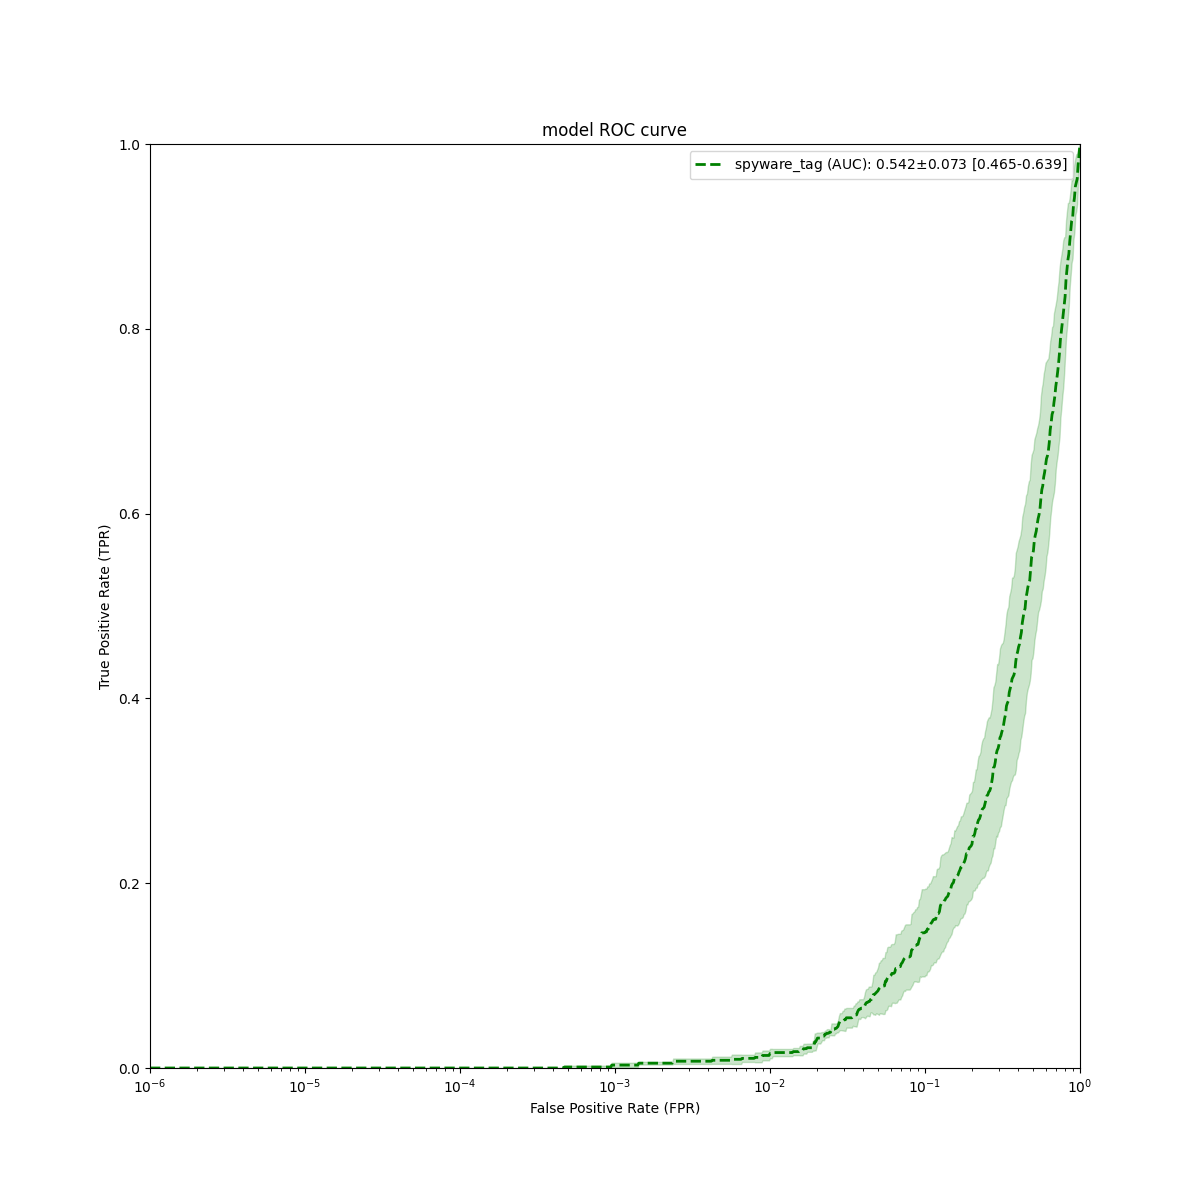
\includegraphics[width=0.6\textwidth]{./results/spyware_tag_roc_aloha.png}
        \vspace*{-0.2cm}
        \caption{ROC curve and AUC statistics of \textBF{ALOHA} model for the \textbf{Spyware Tag}. The line represents the \textit{mean} TPR at a given FPR, while the shaded region represents the \textit{standard deviation}. Statistics were computed over \textBF{3} training runs, each with random parameter initialization.}
        \label{fig:spywareTagRocAloha}
    \end{figure}
}

\newcommand{\spywareTagRocJointEmbedding}{
    \begin{figure}[H]
        \vspace*{-0.5cm}
        \centering
        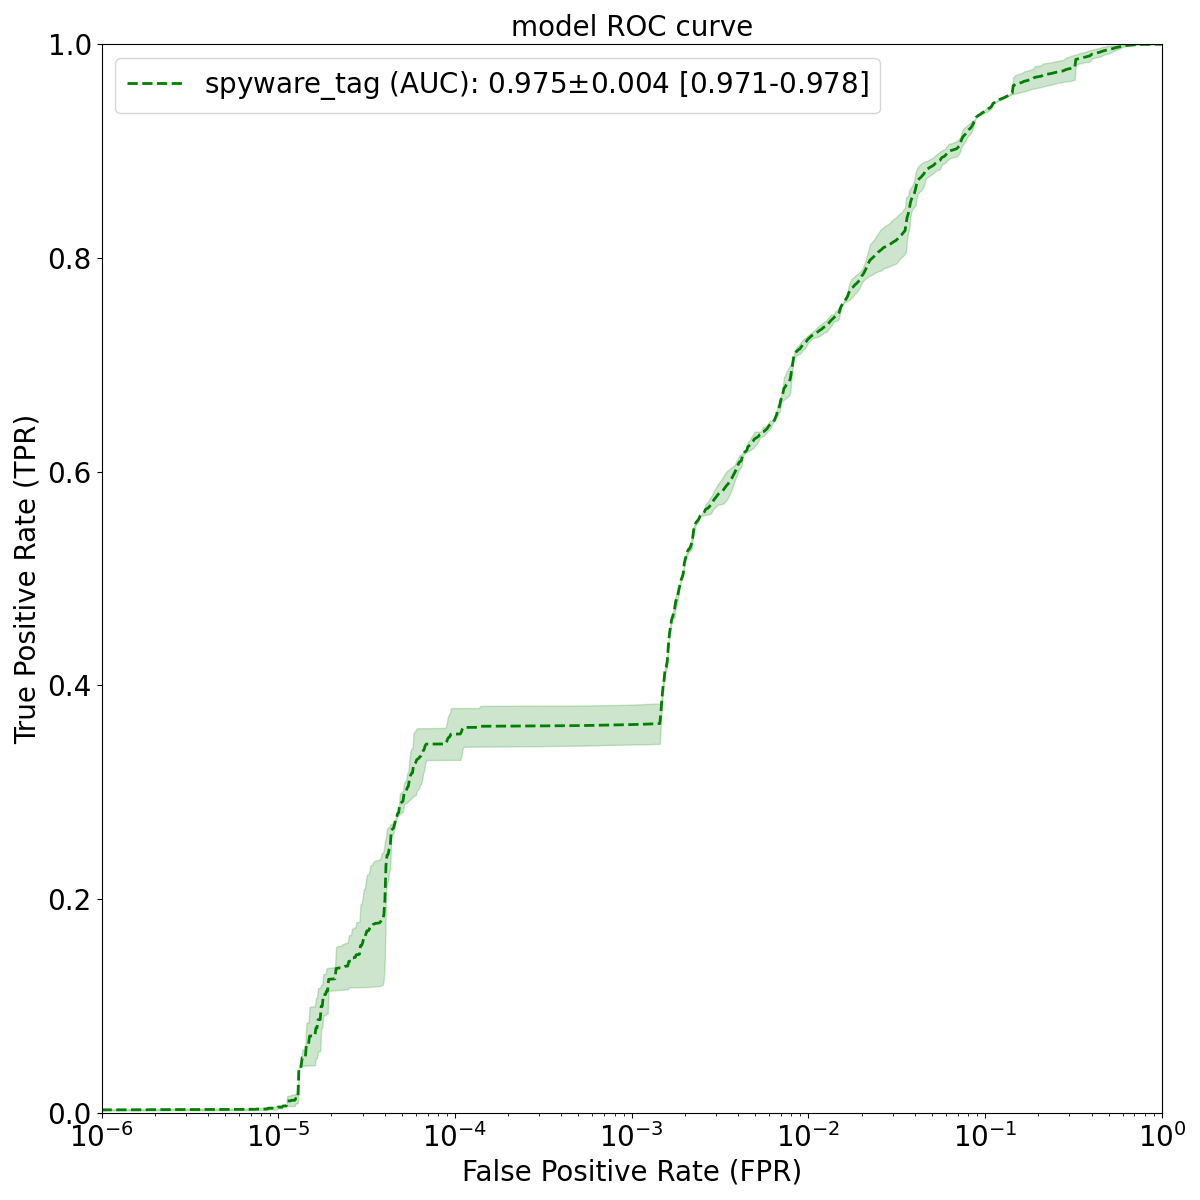
\includegraphics[width=0.6\textwidth]{./results/spyware_tag_roc_jointEmbedding.png}
        \vspace*{-0.2cm}
        \caption{ROC curve and AUC statistics of \textBF{Joint Embedding} model for the \textbf{Spyware Tag}. The line represents the \textit{mean} TPR at a given FPR, while the shaded region represents the \textit{standard deviation}. Statistics were computed over \textBF{3} training runs, each with random parameter initialization.}
        \label{fig:spywareTagRocJointEmbedding}
    \end{figure}
}

\newcommand{\spywareTagRocProposedMethod}{
    \begin{figure}[H]
        \vspace*{-0.5cm}
        \centering
        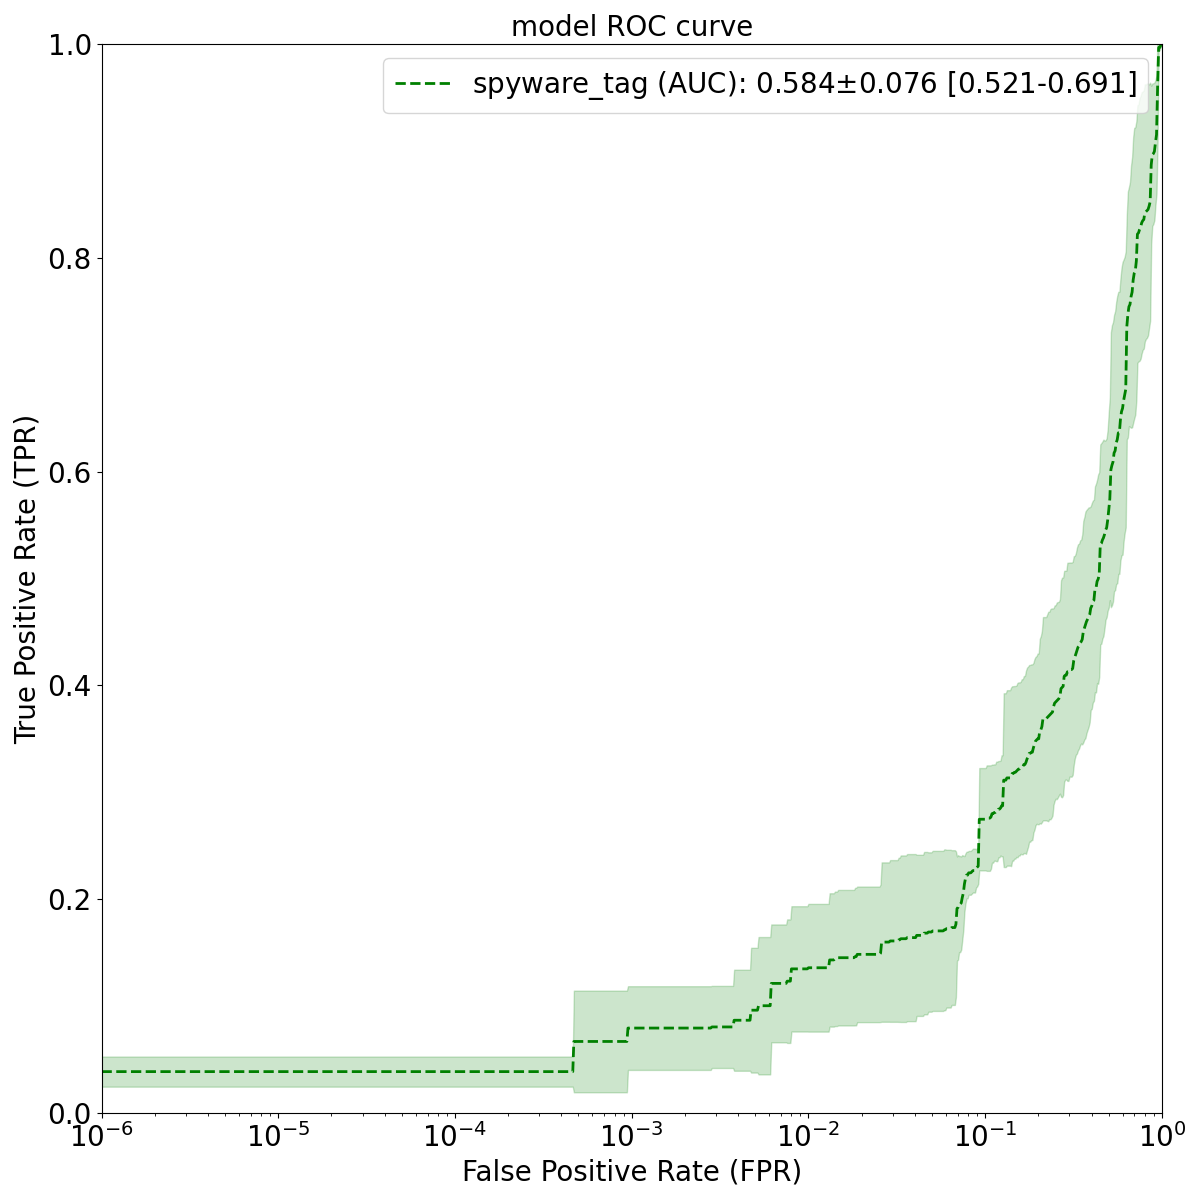
\includegraphics[width=0.6\textwidth]{./results/spyware_tag_roc_proposedModel.png}
        \vspace*{-0.2cm}
        \caption{ROC curve and AUC statistics of \textBF{Proposed Model} for the \textbf{Spyware Tag}. The line represents the \textit{mean} TPR at a given FPR, while the shaded region represents the \textit{standard deviation}. Statistics were computed over \textBF{3} training runs, each with random parameter initialization.}
        \label{fig:spywareTagRocProposedModel}
    \end{figure}
}

%\newcommand{\wormTagResultsAucTable}{
    \begin{table}[H]
        \centering
        \begin{tabular}{|p{2,8cm}||P{2,4cm} P{2,4cm} P{2,4cm}|}
            \hline
            Worm Tag & ALOHA\newline (M/B only) & ALOHA & Proposed\newline Model \\
            \hline
            AUC-ROC & - & 0.562$\pm$0.037 & \textBF{0.648$\pm$0.011} \\
            \hline
        \end{tabular}
        \caption[Worm Tag prediction task AUC-ROC results]{AUC-ROC (Area Under Curve) of the different models for the \textbf{Worm Tag} prediction task. Results were aggregated over \textBF{2} training runs with different weight initializations and minibatch orderings. Best results are shown in \textbf{bold}.} \label{tab:wormTag_auc}
    \end{table}
}

\newcommand{\wormTagResultsAtFprTable}{
    \begin{center}
        \begin{longtable}[c]{|P{3,2cm}||P{1,8cm} P{1,8cm} P{1,8cm} P{1,8cm} P{1,8cm}|}
            \hline
            Worm Tag & \multicolumn{5}{c|}{{FPR}} \\
            & $10^{-5}$ & $10^{-4}$ & $10^{-3}$ & $10^{-2}$ & $10^{-1}$ \\
            \hline
            \endfirsthead

            \caption*{\raggedright ...continued from previous page} \\
            \hline
            Worm Tag & \multicolumn{5}{c|}{\textbf{FPR}} \\
            & $10^{-5}$ & $10^{-4}$ & $10^{-3}$ & $10^{-2}$ & $10^{-1}$ \\
            \hline
            \endhead

            \caption*{\raggedleft ...continued on next page} \\
            \endfoot

            \caption[Worm Tag prediction task results]{Mean and standard deviation results (TPR, Accuracy, Recall, Precision and F1-Score) of the different models for the \textbf{Worm Tag} prediction task at different \textbf{FPR}s (\textit{False Positive Rates}). Results were aggregated over \textBF{2} training runs with different weight initializations and minibatch orderings. Best results are shown in \textbf{bold}. Under \textbf{TPR} results are also presented the percentage reduction in mean detection error and in ROC curve standard deviation introduced by the \textit{Proposed Model} with respect to both \textit{ALOHA} model and \textit{Joint Embedding}.} \label{tab:wormTag_results_at_fpr} \\
            \endlastfoot

            \multicolumn{6}{|c|}{\textbf{TPR}} \\
            \hline
            ALOHA (M/B only) & - & - & - & - & - \\
            ALOHA & 0.010$\pm$0.010 & 0.010$\pm$0.010 & 0.012$\pm$0.012 & 0.012$\pm$0.012 & 0.117$\pm$0.047 \\
            Proposed Model & \textBF{0.021$\pm$0.021} & \textBF{0.021$\pm$0.021} & \textBF{0.021$\pm$0.021} & \textBF{0.031$\pm$0.027} & \textBF{0.238$\pm$0.137} \\
            \hline
            Error Reduction wrt\newline ALOHA (M/B only) & - & - & - & - & - \\
            Error Reduction wrt\newline ALOHA & 1.1\% & 1.1\% & 0.9\% & 1.9\% & 13.7\% \\
            \hline
            Std Reduction wrt\newline ALOHA (M/B only) & - & - & - & - & - \\
            Std Reduction wrt\newline ALOHA & -110.0\% & -110.0\% & -75.0\% & -125.0\% & -191.5\% \\
            \hline
            \multicolumn{6}{|c|}{\textbf{Accuracy}} \\
            \hline
            ALOHA (M/B only) & - & - & - & - & - \\
            ALOHA & 0.896$\pm$0.001 & 0.896$\pm$0.001 & 0.896$\pm$0.001 & \textBF{0.893$\pm$0.004} & 0.819$\pm$0.006 \\
            Proposed Model & \textBF{0.898$\pm$0.002} & \textBF{0.898$\pm$0.002} & 0.897$\pm$0.003 & 0.890$\pm$0.003 & \textBF{0.831$\pm$0.014} \\
            \hline
            \multicolumn{6}{|c|}{\textbf{Recall}} \\
            \hline
            ALOHA (M/B only) & - & - & - & - & - \\
            ALOHA & 0.010$\pm$0.010 & 0.010$\pm$0.010 & 0.012$\pm$0.012 & 0.012$\pm$0.012 & 0.117$\pm$0.047 \\
            Proposed Model & \textBF{0.021$\pm$0.021} & \textBF{0.021$\pm$0.021} & \textBF{0.021$\pm$0.021} & \textBF{0.031$\pm$0.027} & \textBF{0.238$\pm$0.137} \\
            \hline
            \multicolumn{6}{|c|}{\textbf{Precision}} \\
            \hline
            ALOHA (M/B only) & - & - & - & - & - \\
            ALOHA & \textBF{1.000$\pm$0.000} & \textBF{1.000$\pm$0.000} & 0.375$\pm$0.375 & \textBF{0.333$\pm$0.333} & 0.119$\pm$0.043 \\
            Proposed Model & \textBF{1.000$\pm$0.000} & \textBF{1.000$\pm$0.000} & \textBF{0.500$\pm$0.500} & 0.224$\pm$0.181 & \textBF{0.205$\pm$0.099} \\
            \hline
            \multicolumn{6}{|c|}{\textbf{F1 Score}} \\
            \hline
            ALOHA (M/B only) & - & - & - & - & - \\
            ALOHA & 0.019$\pm$0.019 & 0.019$\pm$0.019 & 0.023$\pm$0.023 & 0.023$\pm$0.023 & 0.118$\pm$0.045 \\
            Proposed Model & \textBF{0.041$\pm$0.041} & \textBF{0.041$\pm$0.041} & \textBF{0.041$\pm$0.041} & \textBF{0.055$\pm$0.048} & \textBF{0.220$\pm$0.116} \\
            \hline
        \end{longtable}
    \end{center}
}

\newcommand{\wormTagResultsSummaryTable}{
    \begin{table}[H]
        \centering
        \begin{tabular}{|P{3,2cm}||P{1,8cm} P{1,8cm} P{1,8cm} P{1,8cm} P{1,8cm}|}
            \hline
            \multicolumn{6}{|c|}{Worm Tag (at FPR $=1\%$)} \\
            \hline
            Model & TPR & Accuracy & Precision & Recall & F1 score \\
            \hline
            ALOHA (M/B only) & - & - & - & - & - \\
            ALOHA & 0.012$\pm$0.012 & \textBF{0.893$\pm$0.004} & \textBF{0.333$\pm$0.333} & 0.012$\pm$0.012 & 0.023$\pm$0.023 \\
            Proposed Model & \textBF{0.031$\pm$0.027} & 0.890$\pm$0.003 & 0.224$\pm$0.181 & \textBF{0.031$\pm$0.027} & \textBF{0.055$\pm$0.048} \\
            \hline
        \end{tabular}
        \caption[Summary of Worm Tag prediction task results]{Summary of the mean and standard deviation results of the different models for the \textbf{Worm Tag} prediction task at \textbf{FPR} $=1\%$. Results were aggregated over \textBF{2} training runs with different weight initializations and minibatch orderings. Best results are shown in \textbf{bold}.} \label{tab:wormTag_result_summary}
    \end{table}
}

\newcommand{\wormTagRocAlohaMB}{
    \begin{figure}[H]
        \vspace*{-0.5cm}
        \centering
        \includegraphics[width=0.6\textwidth]{./results/worm_tag_roc_alohaMB.png}
        \vspace*{-0.2cm}
        \caption[Worm Tag prediction task ALOHA (M/B only) ROC curve]{ROC curve and AUC statistics of \textBF{ALOHA (M/B only)} model for the \textbf{Worm Tag}. The line represents the \textit{mean} TPR at a given FPR, while the shaded region represents the \textit{standard deviation}. Statistics were computed over \textBF{2} training runs, each with random parameter initialization.}
        \label{fig:wormTagRocAlohaMB}
    \end{figure}
}

\newcommand{\wormTagRocAloha}{
    \begin{figure}[H]
        \vspace*{-0.5cm}
        \centering
        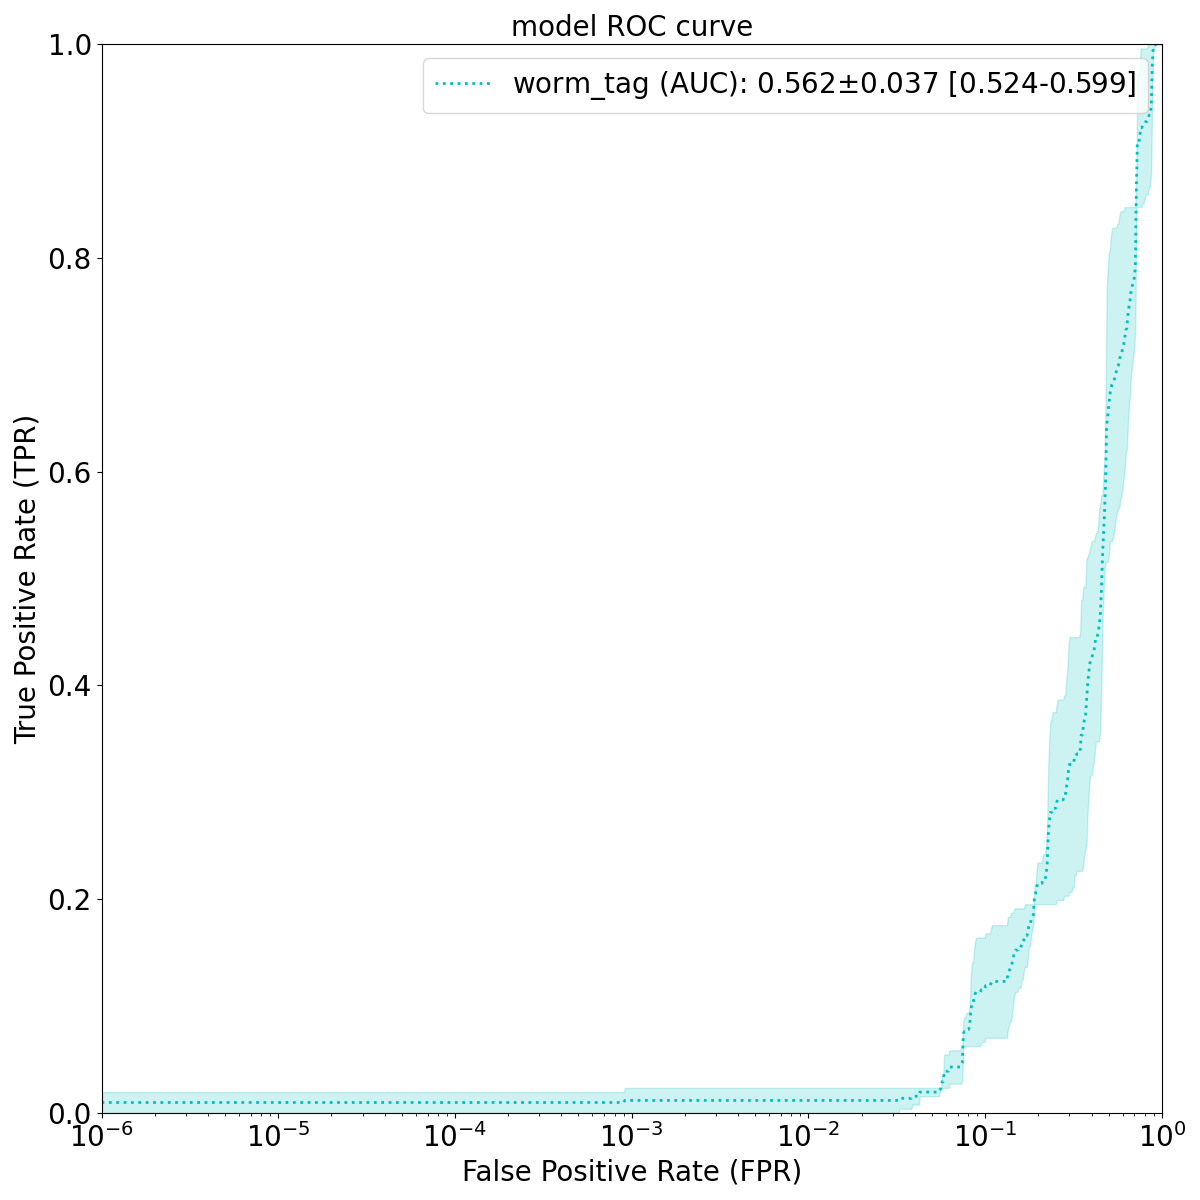
\includegraphics[width=0.6\textwidth]{./results/worm_tag_roc_aloha.png}
        \vspace*{-0.2cm}
        \caption[Worm Tag prediction task ALOHA ROC curve]{ROC curve and AUC statistics of \textBF{ALOHA} model for the \textbf{Worm Tag}. The line represents the \textit{mean} TPR at a given FPR, while the shaded region represents the \textit{standard deviation}. Statistics were computed over \textBF{2} training runs, each with random parameter initialization.}
        \label{fig:wormTagRocAloha}
    \end{figure}
}

\newcommand{\wormTagRocProposedMethod}{
    \begin{figure}[H]
        \vspace*{-0.5cm}
        \centering
        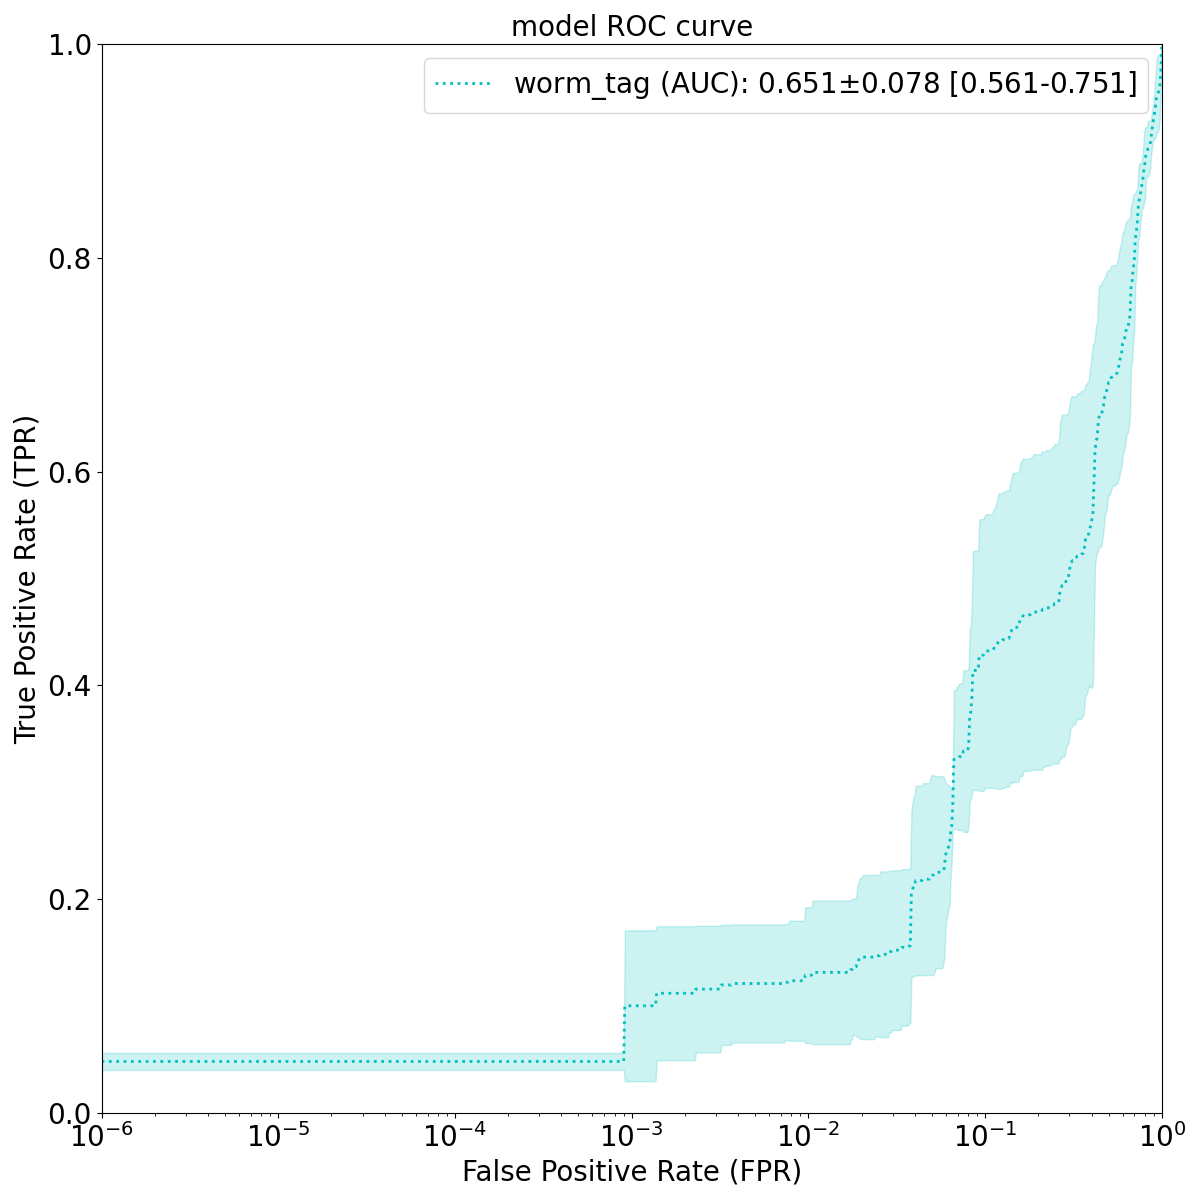
\includegraphics[width=0.6\textwidth]{./results/worm_tag_roc_proposedModel.png}
        \vspace*{-0.2cm}
        \caption[Worm Tag prediction task Proposed Model ROC curve]{ROC curve and AUC statistics of \textBF{Proposed Model} for the \textbf{Worm Tag}. The line represents the \textit{mean} TPR at a given FPR, while the shaded region represents the \textit{standard deviation}. Statistics were computed over \textBF{2} training runs, each with random parameter initialization.}
        \label{fig:wormTagRocProposedModel}
    \end{figure}
}


\newcommand{\meanPerSampleScores}{
    \begin{table}[H]
        \centering
        \begin{tabular}{|P{3,2cm}||P{1,8cm} P{1,8cm} P{1,8cm} P{1,8cm} P{1,8cm}|}
            \hline
            Mean per-sample & \multicolumn{5}{c|}{\textbf{FPR}} \\
            tagging scores & $10^{-5}$ & $10^{-4}$ & $10^{-3}$ & $10^{-2}$ & $10^{-1}$ \\
            \hline
            \multicolumn{6}{|c|}{\textbf{Jaccard Similarity}} \\
            \hline
            ALOHA & 0.718$\pm$0.000 & 0.718$\pm$0.000 & \textBF{0.715$\pm$0.001} & \textBF{0.691$\pm$0.002} & \textBF{0.493$\pm$0.042} \\
            Joint Embedding & 0.718$\pm$0.001 & 0.718$\pm$0.001 & 0.714$\pm$0.001 & 0.676$\pm$0.001 & 0.385$\pm$0.026 \\
            Proposed Model & \textBF{0.719$\pm$0.001} & \textBF{0.719$\pm$0.001} & 0.715$\pm$0.003 & 0.685$\pm$0.001 & 0.370$\pm$0.007 \\
            \hline
            \multicolumn{6}{|c|}{\textbf{Mean per-Sample Accuracy}} \\
            \hline
            ALOHA & \textBF{0.718$\pm$0.000} & \textBF{0.718$\pm$0.000} & \textBF{0.714$\pm$0.001} & \textBF{0.688$\pm$0.002} & \textBF{0.481$\pm$0.040} \\
            Joint Embedding & \textBF{0.718$\pm$0.000} & \textBF{0.718$\pm$0.000} & 0.712$\pm$0.001 & 0.672$\pm$0.000 & 0.364$\pm$0.026 \\
            Proposed Model & \textBF{0.718$\pm$0.000} & \textBF{0.718$\pm$0.000} & 0.713$\pm$0.001 & 0.681$\pm$0.001 & 0.344$\pm$0.005 \\
            \hline
        \end{tabular}
        \caption[Tags prediction task mean per-sample scores]{Mean and standard deviation of mean per-sample tagging results (\textit{Jaccard simialrity} and \textit{mean per-sample accuracy}) for the different models. Results were aggregated over \textBF{2} training runs with different weight initializations and minibatch orderings. Best results are shown in \textbf{bold}.} \label{tab:meanPerSampleScores}
    \end{table}
}

\newcommand{\allMeanRocAloha}{
    \begin{figure}[H]
        \vspace*{-0.5cm}
        \centering
        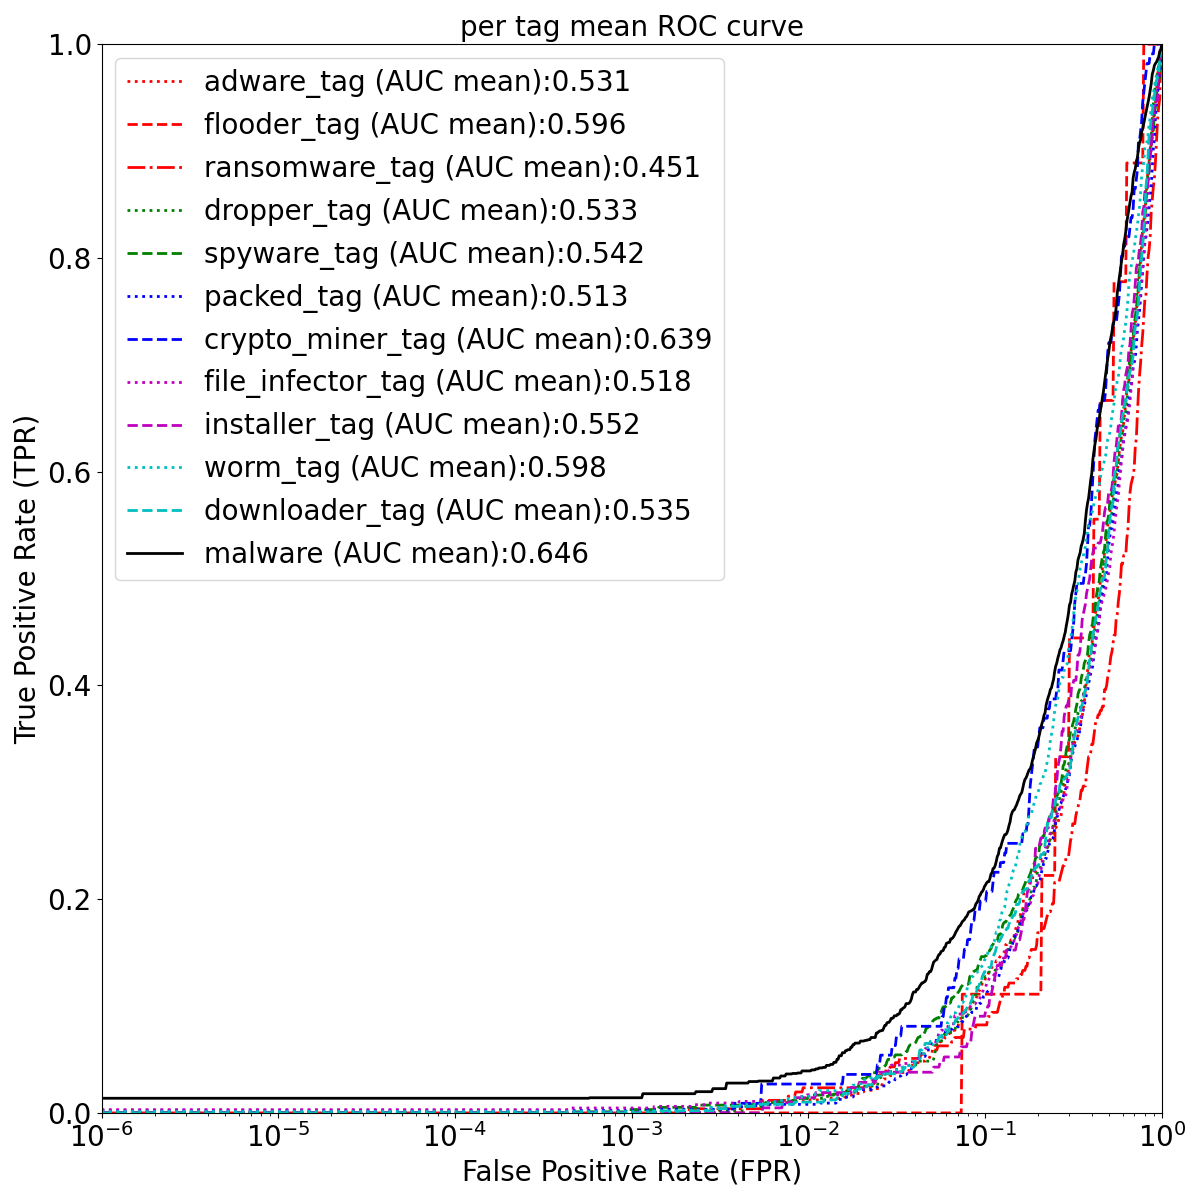
\includegraphics[width=0.6\textwidth]{./results/all_mean_roc_aloha.png}
        \vspace*{-0.2cm}
        \caption[Tags prediction task ALOHA mean ROC curve]{Mean ROC curve and AUC statistics of \textBF{ALOHA} model for the tags/labels. The line represents the \textit{mean} TPR at a given FPR. Statistics were computed over \textBF{2} training runs, each with random parameter initialization.}
        \label{fig:allMeanRocAloha}
    \end{figure}
}

\newcommand{\allMeanRocJointEmbedding}{
    \begin{figure}[H]
        \vspace*{-0.5cm}
        \centering
        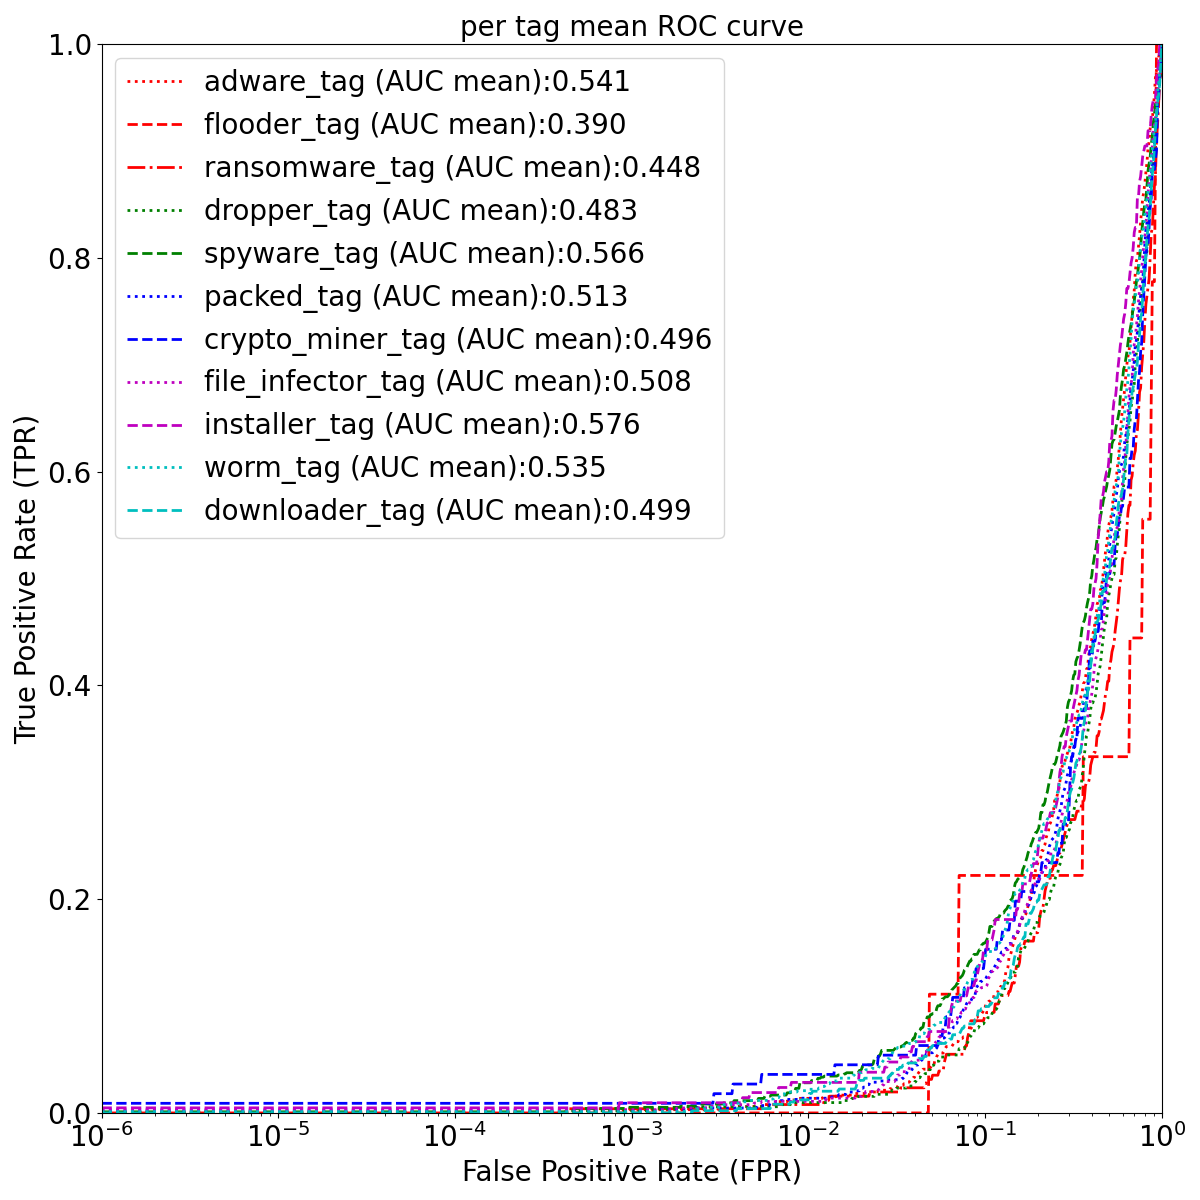
\includegraphics[width=0.6\textwidth]{./results/all_mean_roc_jointEmbedding.png}
        \vspace*{-0.2cm}
        \caption[Tags prediction task Joint Embedding mean ROC curve]{Mean ROC curve and AUC statistics of \textBF{Joint Embedding} model for all tags/labels. The line represents the \textit{mean} TPR at a given FPR. Statistics were computed over \textBF{2} training runs, each with random parameter initialization.}
        \label{fig:allMeanRocJointEmbedding}
    \end{figure}
}

\newcommand{\allMeanRocProposedModel}{
    \begin{figure}[H]
        \vspace*{-0.5cm}
        \centering
        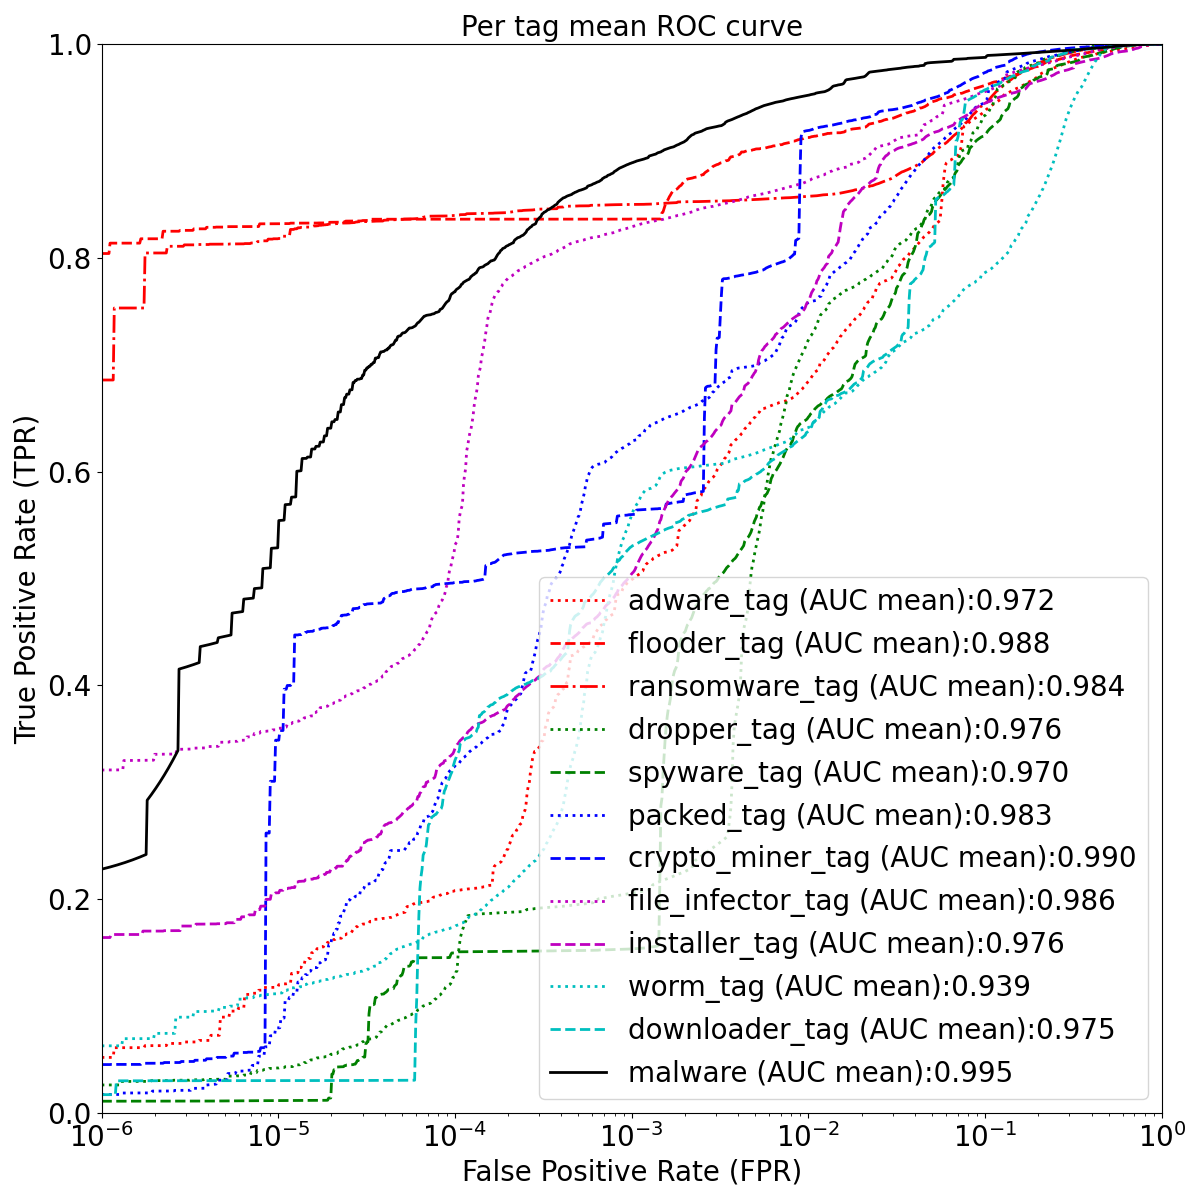
\includegraphics[width=0.6\textwidth]{./results/all_mean_roc_proposedModel.png}
        \vspace*{-0.2cm}
        \caption[Tags prediction task Proposed Model mean ROC curve]{Mean ROC curve and AUC statistics of \textBF{Proposed Model} for the tags/labels. The line represents the \textit{mean} TPR at a given FPR. Statistics were computed over \textBF{2} training runs, each with random parameter initialization.}
        \label{fig:allMeanRocProposedModel}
    \end{figure}
}
\newcommand{\MrrAndMapResultsTable}{
    \begin{table}[H]
        \centering
        \begin{tabular}{|P{2,8cm}||P{2,2cm} P{2,2cm} P{2,2cm} P{2,2cm}|}
            \hline
            & ALOHA (M/B only) & ALOHA & Joint Embedding & Proposed Model \\
            \hline
            MRR & 0.254$\pm$0.015 & \textBF{0.259$\pm$0.008} & 0.253$\pm$0.012 & 0.253$\pm$0.010 \\
            MAP & 0.106$\pm$0.001 & \textBF{0.106$\pm$0.000} & \textBF{0.106$\pm$0.000} & \textBF{0.106$\pm$0.000} \\
            \hline
        \end{tabular}
        \caption[Family ranking MRR and MAP scores]{Mean and standard deviation MRR (Mean Reciprocal Rank) and MAP (Mean Average Precision) results for the different models on the Family Ranking task. Results were aggregated over \textBF{3} training runs with different weight initializations and minibatch orderings. Best results are shown in \textbf{bold}.} \label{tab:MrrAndMapResults}
    \end{table}
}

\newcommand{\maxApExampleRankTable}{
    \begin{table}[H]
        \centering
        \begin{tabular}{|P{1,8cm}||P{1,7cm} P{1,2cm} P{2cm}|P{1,7cm} P{1,2cm} P{2cm}|}
            \hline
            Max AP & \multicolumn{3}{c|}{ALOHA (M/B)} & \multicolumn{3}{c|}{ALOHA} \\
            & Sha256 & Label & Family & Sha256 & Label & Family \\
            \hline
            Query & 24133d.. & 0 & formbook & e3639a.. & 0 & formbook \\
            \hline
            0 & 8fea1e.. & 3 & quakbot & \textBF{6f16d3}.. & \textBF{0} & \textBF{formbook} \\
			1 & \textBF{02ad1e}.. & \textBF{0} & \textBF{formbook} & \textBF{0655ee}.. & \textBF{0} & \textBF{formbook} \\
			2 & \textBF{8da806}.. & \textBF{0} & \textBF{formbook} & \textBF{40f8cf}.. & \textBF{0} & \textBF{formbook} \\
			3 & 0c95f0.. & 8 & guloader & \textBF{f7c1ec}.. & \textBF{0} & \textBF{formbook} \\
			4 & 95fa71.. & 9 & avemariarat & 620c36.. & 2 & gozi \\
			5 & 4b8466.. & 6 & remcosrat & 38e003.. & 6 & remcosrat \\
			6 & \textBF{191008}.. & \textBF{0} & \textBF{formbook} & \textBF{93e548}.. & \textBF{0} & \textBF{formbook} \\
			7 & 768da5.. & 9 & avemariarat & 1ddaae.. & 4 & loki \\
			8 & \textBF{e92575}.. & \textBF{0} & \textBF{formbook} & 5b9f32.. & 3 & quakbot \\
			9 & f0cae3.. & 3 & quakbot & 83d036.. & 4 & loki \\
            \hline
            Max AP & \multicolumn{3}{c|}{0.186} & \multicolumn{3}{c|}{0.174} \\
            \hline
            Next & \multicolumn{3}{c|}{position 14} & \multicolumn{3}{c|}{position 10} \\
            \hline
            \hline
            Max AP & \multicolumn{3}{c|}{Joint Embedding} & \multicolumn{3}{c|}{Proposed Model} \\
            & Sha256 & Label & Family & Sha256 & Label & Family \\
            \hline
            Query & c0a92a.. & 6 & remcosrat & 389ec4.. & 7 & trickbot \\
            \hline
            0 & \textBF{21f9ef}.. & \textBF{6} & \textBF{remcosrat} & \textBF{aa447e}.. & \textBF{7} & \textBF{trickbot} \\
			1 & \textBF{49c7a5}.. & \textBF{6} & \textBF{remcosrat} & \textBF{cbe743}.. & \textBF{7} & \textBF{trickbot} \\
			2 & f75cb4.. & 2 & gozi & 8dc3da.. & 6 & remcosrat \\
			3 & \textBF{91b004}.. & \textBF{6} & \textBF{remcosrat} & \textBF{e37438}.. & \textBF{7} & \textBF{trickbot} \\
			4 & 2d54d3.. & 3 & quakbot & \textBF{2cadf2}.. & \textBF{7} & \textBF{trickbot} \\
			5 & f86765.. & 9 & avemariarat & 545bc3.. & 8 & guloader \\
			6 & 0ea373.. & 0 & formbook & \textBF{b56a1e}.. & \textBF{7} & \textBF{trickbot} \\
			7 & \textBF{4a9558}.. & \textBF{6} & \textBF{remcosrat} & e14108.. & 6 & remcosrat \\
			8 & 019f79.. & 7 & trickbot & 80e880.. & 2 & gozi \\
			9 & a2f8c1.. & 9 & avemariarat & \textBF{4688b8}.. & \textBF{7} & \textBF{trickbot} \\
            \hline
            Max AP & \multicolumn{3}{c|}{0.190} & \multicolumn{3}{c|}{0.183} \\
            \hline
            Next & \multicolumn{3}{c|}{position 11} & \multicolumn{3}{c|}{position 17} \\
            \hline
        \end{tabular}
        \caption[Family ranking max AP example]{\textBF{ALOHA (M/B) Embedding}, \textBF{ALOHA}, \textBF{Joint Embedding} and \textBF{Proposed Model} example rankings (limited to the first 10 samples) having the maximum Average Precision (max AP). The elements matching the query sample are shown in \textbf{bold}. The last line of each table indicates the position in the ranking where to find the next element belonging to the same family as the query sample.} \label{tab:maxApExampleRank}
    \end{table}
}

\newcommand{\maxRrExampleRankTable}{
    \begin{table}[H]
        \centering
        \begin{tabular}{|P{1,8cm}||P{1,7cm} P{1,2cm} P{2cm}|P{1,7cm} P{1,2cm} P{2cm}|}
            \hline
            Max RR & \multicolumn{3}{c|}{ALOHA (M/B)} & \multicolumn{3}{c|}{ALOHA} \\
            & Sha256 & Label & Family & Sha256 & Label & Family \\
            \hline
            Query & 228f0e.. & 0 & formbook & bcec95.. & 0 & formbook \\
            \hline
            0 & \textBF{f51577}.. & \textBF{0} & \textBF{formbook} & \textBF{7b30aa}.. & \textBF{0} & \textBF{formbook} \\
			1 & d7ece5.. & 3 & quakbot & 2edfad.. & 8 & guloader \\
			2 & 040062.. & 4 & loki & ecdf7d.. & 9 & avemariarat \\
			3 & 80b83b.. & 1 & agenttesla & 74fb06.. & 3 & quakbot \\
			4 & add45f.. & 6 & remcosrat & 0fea0b.. & 7 & trickbot \\
			5 & 608a6d.. & 8 & guloader & 3d4f29.. & 3 & quakbot \\
			6 & 3cb853.. & 6 & remcosrat & b73730.. & 7 & trickbot \\
			7 & fb120a.. & 6 & remcosrat & acf60e.. & 4 & loki \\
			8 & 60984e.. & 1 & agenttesla & a60e97.. & 4 & loki \\
			9 & 457344.. & 6 & remcosrat & 3b2629.. & 7 & trickbot \\
            \hline
            Max RR & \multicolumn{3}{c|}{1.000} & \multicolumn{3}{c|}{1.000} \\
            \hline
            Next & \multicolumn{3}{c|}{position 10} & \multicolumn{3}{c|}{position 11} \\
            \hline
            \hline
            Max RR & \multicolumn{3}{c|}{Joint Embedding} & \multicolumn{3}{c|}{Proposed Model} \\
            & Sha256 & Label & Family & Sha256 & Label & Family \\
            \hline
            Query & 32897c.. & 2 & gozi & 807414.. & 1 & agenttesla \\
            \hline
            0 & \textBF{b4e412}.. & \textBF{2} & \textBF{gozi} & \textBF{d6c10d}.. & \textBF{1} & \textBF{agenttesla} \\
			1 & 0dac03.. & 7 & trickbot & d0dbb5.. & 7 & trickbot \\
			2 & 300ec7.. & 7 & trickbot & 876680.. & 2 & gozi \\
			3 & d9afac.. & 7 & trickbot & 6dba26.. & 7 & trickbot \\
			4 & b1a303.. & 0 & formbook & bd91fc.. & 8 & guloader \\
			5 & b71dc1.. & 7 & trickbot & a31584.. & 6 & remcosrat \\
			6 & 774cff.. & 3 & quakbot & df907a.. & 5 & heodo \\
			7 & 1c8aaa.. & 1 & agenttesla & 3763ee.. & 9 & avemariarat \\
			8 & a6d3dc.. & 1 & agenttesla & 277238.. & 0 & formbook \\
			9 & d01615.. & 1 & agenttesla & 3ad3d1.. & 5 & heodo \\
            \hline
            Max RR & \multicolumn{3}{c|}{1.000} & \multicolumn{3}{c|}{1.000} \\
            \hline
            Next & \multicolumn{3}{c|}{position 12} & \multicolumn{3}{c|}{position 14} \\
            \hline
        \end{tabular}
        \caption[Family ranking max RR example]{\textBF{ALOHA (M/B) Embedding}, \textBF{ALOHA}, \textBF{Joint Embedding} and \textBF{Proposed Model} example rankings (limited to the first 10 samples) having the maximum Reciprocal Rank (max RR). The elements matching the query sample are shown in \textbf{bold}. The last line of each table indicates the position in the ranking where to find the next element belonging to the same family as the query sample.} \label{tab:maxRrExampleRank}
    \end{table}
}
\newcommand{\minApExampleRankTable}{
    \begin{table}[H]
        \centering
        \begin{tabular}{|P{1,8cm}||P{1,7cm} P{1,2cm} P{2cm}|P{1,7cm} P{1,2cm} P{2cm}|}
            \hline
            Min AP & \multicolumn{3}{c|}{ALOHA (M/B)} & \multicolumn{3}{c|}{ALOHA} \\
            & Sha256 & Label & Family & Sha256 & Label & Family \\
            \hline
            Query & f9b156.. & 2 & gozi & ef89d3.. & 8 & guloader \\
            \hline
            0 & c7fc61.. & 6 & remcosrat & 246a1e.. & 3 & quakbot \\
			1 & a5ebcb.. & 5 & heodo & 4a9e32.. & 5 & heodo \\
			2 & 494519.. & 5 & heodo & 84353f.. & 5 & heodo \\
			3 & 4469b2.. & 3 & quakbot & f0125d.. & 2 & gozi \\
			4 & e0c023.. & 0 & formbook & e0e601.. & 1 & agenttesla \\
			5 & a3f0b1.. & 7 & trickbot & 0e20f3.. & 4 & loki \\
			6 & c27598.. & 5 & heodo & 357ab6.. & 6 & remcosrat \\
			7 & 830072.. & 7 & trickbot & f39db6.. & 9 & avemariarat \\
			8 & ca90a8.. & 6 & remcosrat & a98b59.. & 5 & heodo \\
			9 & 341186.. & 7 & trickbot & 719219.. & 7 & trickbot \\
            \hline
            Min AP & \multicolumn{3}{c|}{0.062} & \multicolumn{3}{c|}{0.062} \\
            \hline
            Next & \multicolumn{3}{c|}{position 20} & \multicolumn{3}{c|}{position 39} \\
            \hline
            \hline
            Min AP & \multicolumn{3}{c|}{Joint Embedding} & \multicolumn{3}{c|}{Proposed Model} \\
            & Sha256 & Label & Family & Sha256 & Label & Family \\
            \hline
            Query & c89a67.. & 7 & trickbot & e619c7.. & 3 & quakbot \\
            \hline
            0 & d99c4c.. & 5 & heodo & 71cb97.. & 0 & formbook \\
			1 & b34153.. & 5 & heodo & 10f1ad.. & 1 & agenttesla \\
			2 & 868b30.. & 2 & gozi & 1f1f38.. & 2 & gozi \\
			3 & 3a5181.. & 8 & guloader & 74499f.. & 1 & agenttesla \\
			4 & 6cf9e4.. & 4 & loki & d75380.. & 6 & remcosrat \\
			5 & cf36fa.. & 8 & guloader & d0f6f2.. & 0 & formbook \\
			6 & f2a200.. & 2 & gozi & 7b30aa.. & 0 & formbook \\
			7 & c8eaf6.. & 0 & formbook & 0d0364.. & 6 & remcosrat \\
			8 & e2c837.. & 2 & gozi & ac0afc.. & 6 & remcosrat \\
			9 & 1331f9.. & 0 & formbook & d3d0a5.. & 0 & formbook \\
            \hline
            Min AP & \multicolumn{3}{c|}{0.063} & \multicolumn{3}{c|}{0.065} \\
            \hline
            Next & \multicolumn{3}{c|}{position 67} & \multicolumn{3}{c|}{position 49} \\
            \hline
        \end{tabular}
        \caption[Family ranking min AP example]{\textBF{ALOHA (M/B) Embedding}, \textBF{ALOHA}, \textBF{Joint Embedding} and \textBF{Proposed Model} example rankings (limited to the first 10 samples) having the minimum Average Precision (max AP). The elements matching the query sample are shown in \textbf{bold}. The last line of each table indicates the position in the ranking where to find the next element belonging to the same family as the query sample.} \label{tab:minApExampleRank}
    \end{table}
}

\newcommand{\minRrExampleRankTable}{
    \begin{table}[H]
        \centering
        \begin{tabular}{|P{1,8cm}||P{1,7cm} P{1,2cm} P{2cm}|P{1,7cm} P{1,2cm} P{2cm}|}
            \hline
            Min RR & \multicolumn{3}{c|}{ALOHA (M/B)} & \multicolumn{3}{c|}{ALOHA} \\
            & Sha256 & Label & Family & Sha256 & Label & Family \\
            \hline
            Query & 5f9b8c.. & 8 & guloader & b845b6.. & 1 & agenttesla \\
            \hline
            0 & 90770a.. & 4 & loki & 6c3efe.. & 5 & heodo \\
			1 & f70695.. & 5 & heodo & a09ad5.. & 0 & formbook \\
			2 & 1a778e.. & 5 & heodo & bad7c7.. & 2 & gozi \\
			3 & b0ea42.. & 4 & loki & 18498c.. & 7 & trickbot \\
			4 & 0d77b2.. & 9 & avemariarat & b840f4.. & 0 & formbook \\
			5 & 300dd4.. & 0 & formbook & 3bfc15.. & 6 & remcosrat \\
			6 & a98ba3.. & 0 & formbook & 76cf64.. & 6 & remcosrat \\
			7 & cb5547.. & 6 & remcosrat & 8b6690.. & 9 & avemariarat \\
			8 & 86a419.. & 9 & avemariarat & 31cce8.. & 8 & guloader \\
			9 & 3c2770.. & 2 & gozi & c15a76.. & 2 & gozi \\
            \hline
            Min RR & \multicolumn{3}{c|}{0.008} & \multicolumn{3}{c|}{0.009} \\
            \hline
            Next & \multicolumn{3}{c|}{position 128} & \multicolumn{3}{c|}{position 113} \\
            \hline
            \hline
            Min RR & \multicolumn{3}{c|}{Joint Embedding} & \multicolumn{3}{c|}{Proposed Model} \\
            & Sha256 & Label & Family & Sha256 & Label & Family \\
            \hline
            Query & 4a9e32.. & 5 & heodo & dbfdd9.. & 8 & guloader \\
            \hline
            0 & cedbc9.. & 7 & trickbot & 861dd1.. & 2 & gozi \\
			1 & b48f0a.. & 6 & remcosrat & dca295.. & 3 & quakbot \\
			2 & 174bce.. & 2 & gozi & c89194.. & 1 & agenttesla \\
			3 & 8af585.. & 9 & avemariarat & feb0ce.. & 1 & agenttesla \\
			4 & 4e8a4f.. & 3 & quakbot & 26ee0a.. & 1 & agenttesla \\
			5 & 0558ff.. & 9 & avemariarat & 32e56e.. & 2 & gozi \\
			6 & 7f3487.. & 0 & formbook & 510e00.. & 3 & quakbot \\
			7 & a6e4d5.. & 8 & guloader & d21f7c.. & 6 & remcosrat \\
			8 & 850c25.. & 1 & agenttesla & c3df57.. & 0 & formbook \\
			9 & 853d14.. & 6 & remcosrat & 27bc44.. & 3 & quakbot \\
            \hline
            Min RR & \multicolumn{3}{c|}{0.011} & \multicolumn{3}{c|}{0.009} \\
            \hline
            Next & \multicolumn{3}{c|}{position 94} & \multicolumn{3}{c|}{position 106} \\
            \hline
        \end{tabular}
        \caption[Family ranking min RR example]{\textBF{ALOHA (M/B) Embedding}, \textBF{ALOHA}, \textBF{Joint Embedding} and \textBF{Proposed Model} example rankings (limited to the first 10 samples) having the minimum Reciprocal Rank (max RR). The elements matching the query sample are shown in \textbf{bold}. The last line of each table indicates the position in the ranking where to find the next element belonging to the same family as the query sample.} \label{tab:minRrExampleRank}
    \end{table}
}
\newcommand{\freshResultsAucTable}{
    \begin{center}
        \begin{longtable}[c]{|p{2,8cm}||p{2,8cm} p{2,8cm} p{2,8cm}|}
            \hline
            AUC-ROC & ALOHA & Joint Embedding & Proposed Model \\
            \hline
            \endfirsthead

            \caption*{\raggedright ...continued from previous page} \\
            \hline
            AUC-ROC & ALOHA & Joint Embedding & Proposed Model \\
            \hline
            \endhead

            \caption*{\raggedleft ...continued on next page} \\
            \endfoot

            \caption{Mean and standard deviation AUC-ROC (Area Under Curve) of the different models for the the prediction of the different families on fresh dataset samples. Results were aggregated over \textBF{3} training runs with different weight initializations and minibatch orderings. Best results are shown in \textbf{bold}.} \label{tab:families_aucs}
            \endlastfoot

            Agenttesla & - & \textBF{0.631$\pm$0.046} & 0.614$\pm$0.063 \\
            Avemariarat & - & \textBF{0.555$\pm$0.022} & 0.539$\pm$0.031 \\
            Azorult & - & \textBF{0.598$\pm$0.036} & 0.573$\pm$0.050 \\
            Formbook & - & \textBF{0.555$\pm$0.056} & 0.543$\pm$0.020 \\
            Heodo & - & \textBF{0.838$\pm$0.017} & 0.803$\pm$0.017 \\
            Loki & - & \textBF{0.570$\pm$0.035} & 0.553$\pm$0.045 \\
            Masslogger & - & 0.538$\pm$0.025 & \textBF{0.589$\pm$0.010} \\
            Netwire & - & \textBF{0.527$\pm$0.005} & 0.500$\pm$0.021 \\
            Njrat & - & \textBF{0.746$\pm$0.017} & 0.736$\pm$0.008 \\
            Remcorsat & - & \textBF{0.560$\pm$0.016} & 0.539$\pm$0.032 \\
            \hline
        \end{longtable}
    \end{center}
}

\newcommand{\freshResultsSummaryTable}{
    \begin{center}
        \begin{longtable}[c]{|p{3,2cm}||p{1,8cm} p{1,8cm} p{1,8cm} p{1,8cm} p{1,8cm}|}
            \hline
            & TPR & Accuracy & Precision & Recall & F1 score \\
            \hline
            \endfirsthead

            \caption*{\raggedright ...continued from previous page} \\
            \hline
            & TPR & Accuracy & Precision & Recall & F1 score \\
            \hline
            \endhead

            \caption*{\raggedleft ...continued on next page} \\
            \endfoot

            \caption{Summary of the mean and standard deviation results of the different models for the prediction of the different families on fresh dataset samples at \textbf{FPR} $=1\%$. Results were aggregated over \textBF{3} training runs with different weight initializations and minibatch orderings. Best results are shown in \textbf{bold}.} \label{tab:fresh_results_summary}
            \endlastfoot

            \multicolumn{6}{|c|}{\textbf{Agenttesla} (at FPR $=1\%$)} \\
            \hline
            Joint Embedding & \textBF{0.020$\pm$0.005} & \textBF{0.900$\pm$0.000} & \textBF{1.000$\pm$0.000} & \textBF{0.000$\pm$0.000} & \textBF{0.000$\pm$0.000} \\
            Proposed Model & 0.019$\pm$0.008 & \textBF{0.900$\pm$0.000} & \textBF{1.000$\pm$0.000} & \textBF{0.000$\pm$0.000} & \textBF{0.000$\pm$0.000} \\
            \hline
            \multicolumn{6}{|c|}{\textbf{Avemariarat} (at FPR $=1\%$)} \\
            \hline
            Joint Embedding & \textBF{0.016$\pm$0.003} & \textBF{0.900$\pm$0.000} & \textBF{1.000$\pm$0.000} & \textBF{0.000$\pm$0.000} & \textBF{0.000$\pm$0.000} \\
            Proposed Model & 0.013$\pm$0.003 & \textBF{0.900$\pm$0.000} & \textBF{1.000$\pm$0.000} & \textBF{0.000$\pm$0.000} & \textBF{0.000$\pm$0.000} \\
            \hline
            \multicolumn{6}{|c|}{\textbf{Azorult} (at FPR $=1\%$)} \\
            \hline
            Joint Embedding & \textBF{0.016$\pm$0.001} & \textBF{0.900$\pm$0.000} & \textBF{1.000$\pm$0.000} & \textBF{0.000$\pm$0.000} & \textBF{0.000$\pm$0.000} \\
            Proposed Model & 0.014$\pm$0.003 & \textBF{0.900$\pm$0.000} & \textBF{1.000$\pm$0.000} & \textBF{0.000$\pm$0.000} & \textBF{0.000$\pm$0.000} \\
            \hline
            \multicolumn{6}{|c|}{\textbf{Formbook} (at FPR $=1\%$)} \\
            \hline
            Joint Embedding & \textBF{0.015$\pm$0.005} & \textBF{0.900$\pm$0.000} & \textBF{1.000$\pm$0.000} & \textBF{0.000$\pm$0.000} & \textBF{0.000$\pm$0.000} \\
            Proposed Model & 0.012$\pm$0.001 & \textBF{0.900$\pm$0.000} & \textBF{1.000$\pm$0.000} & \textBF{0.000$\pm$0.000} & \textBF{0.000$\pm$0.000} \\
            \hline
            \multicolumn{6}{|c|}{\textbf{Heodo} (at FPR $=1\%$)} \\
            \hline
            Joint Embedding & \textBF{0.045$\pm$0.012} & \textBF{0.900$\pm$0.000} & \textBF{1.000$\pm$0.000} & \textBF{0.000$\pm$0.000} & \textBF{0.000$\pm$0.000} \\
            Proposed Model & 0.039$\pm$0.002 & \textBF{0.900$\pm$0.000} & \textBF{1.000$\pm$0.000} & \textBF{0.000$\pm$0.000} & \textBF{0.000$\pm$0.000} \\
            \hline
            \multicolumn{6}{|c|}{\textbf{Loki} (at FPR $=1\%$)} \\
            \hline
            Joint Embedding & \textBF{0.016$\pm$0.004} & \textBF{0.900$\pm$0.000} & \textBF{1.000$\pm$0.000} & \textBF{0.000$\pm$0.000} & \textBF{0.000$\pm$0.000} \\
            Proposed Model & 0.012$\pm$0.002 & \textBF{0.900$\pm$0.000} & \textBF{1.000$\pm$0.000} & \textBF{0.000$\pm$0.000} & \textBF{0.000$\pm$0.000} \\
            \hline
            \multicolumn{6}{|c|}{\textbf{Masslogger} (at FPR $=1\%$)} \\
            \hline
            Joint Embedding & 0.013$\pm$0.002 & \textBF{0.900$\pm$0.000} & \textBF{1.000$\pm$0.000} & \textBF{0.000$\pm$0.000} & \textBF{0.000$\pm$0.000} \\
            Proposed Model & \textBF{0.016$\pm$0.001} & \textBF{0.900$\pm$0.000} & \textBF{1.000$\pm$0.000} & \textBF{0.000$\pm$0.000} & \textBF{0.000$\pm$0.000} \\
            \hline
            \multicolumn{6}{|c|}{\textbf{Netwire} (at FPR $=1\%$)} \\
            \hline
            Joint Embedding & \textBF{0.012$\pm$0.001} & \textBF{0.900$\pm$0.000} & \textBF{1.000$\pm$0.000} & \textBF{0.000$\pm$0.000} & \textBF{0.000$\pm$0.000} \\
            Proposed Model & 0.010$\pm$0.001 & \textBF{0.900$\pm$0.000} & \textBF{1.000$\pm$0.000} & \textBF{0.000$\pm$0.000} & \textBF{0.000$\pm$0.000} \\
            \hline
            \multicolumn{6}{|c|}{\textbf{Njrat} (at FPR $=1\%$)} \\
            \hline
            Joint Embedding & \textBF{0.030$\pm$0.002} & \textBF{0.900$\pm$0.000} & \textBF{1.000$\pm$0.000} & \textBF{0.000$\pm$0.000} & \textBF{0.000$\pm$0.000} \\
            Proposed Model & 0.026$\pm$0.004 & \textBF{0.900$\pm$0.000} & \textBF{1.000$\pm$0.000} & \textBF{0.000$\pm$0.000} & \textBF{0.000$\pm$0.000} \\
            \hline
            \multicolumn{6}{|c|}{\textbf{Remcorsat} (at FPR $=1\%$)} \\
            \hline
            Joint Embedding & \textBF{0.015$\pm$0.002} & \textBF{0.900$\pm$0.000} & \textBF{1.000$\pm$0.000} & \textBF{0.000$\pm$0.000} & \textBF{0.000$\pm$0.000} \\
            Proposed Model & 0.012$\pm$0.002 & \textBF{0.900$\pm$0.000} & \textBF{1.000$\pm$0.000} & \textBF{0.000$\pm$0.000} & \textBF{0.000$\pm$0.000} \\
            \hline
        \end{longtable}
    \end{center}
}

\newcommand{\allMeanFreshRocJointEmbedding}{
    \begin{figure}[H]
        \vspace*{-0.5cm}
        \centering
        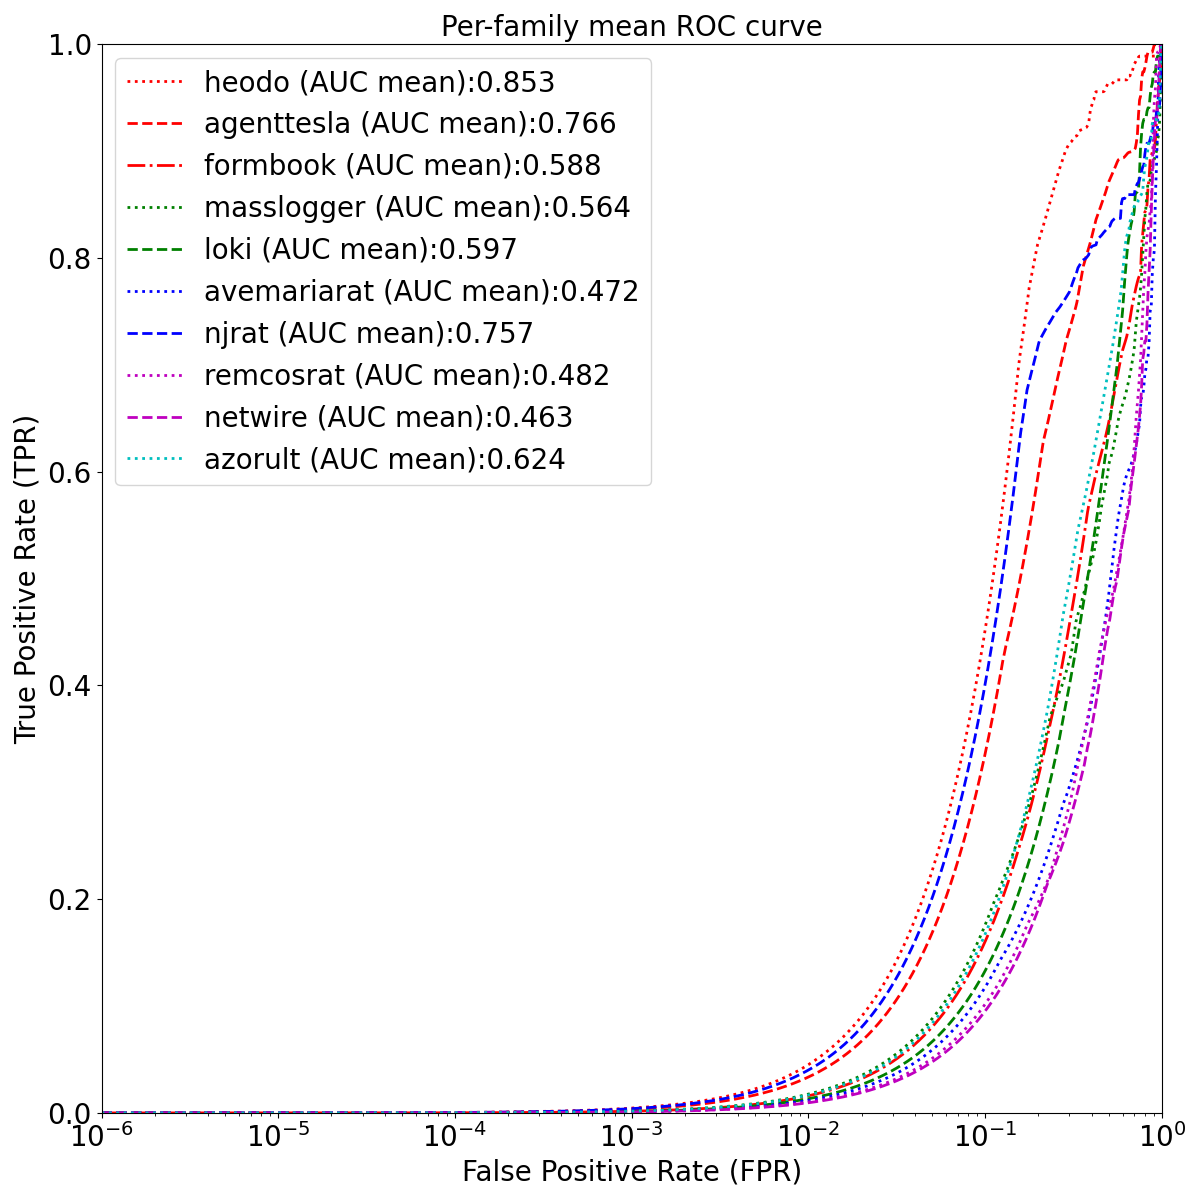
\includegraphics[width=0.6\textwidth]{./results/all_mean_fresh_roc_jointEmbedding.png}
        \vspace*{-0.2cm}
        \caption{Mean ROC curve and AUC statistics of \textBF{Joint Embedding} model for the prediction of all families on fresh dataset samples. The line represents the \textit{mean} TPR at a given FPR. Statistics were computed over \textBF{3} training runs, each with random parameter initialization.}
        \label{fig:allMeanFreshRocJointEmbedding}
    \end{figure}
}

\newcommand{\allMeanFreshRocProposedModel}{
    \begin{figure}[H]
        \vspace*{-0.5cm}
        \centering
        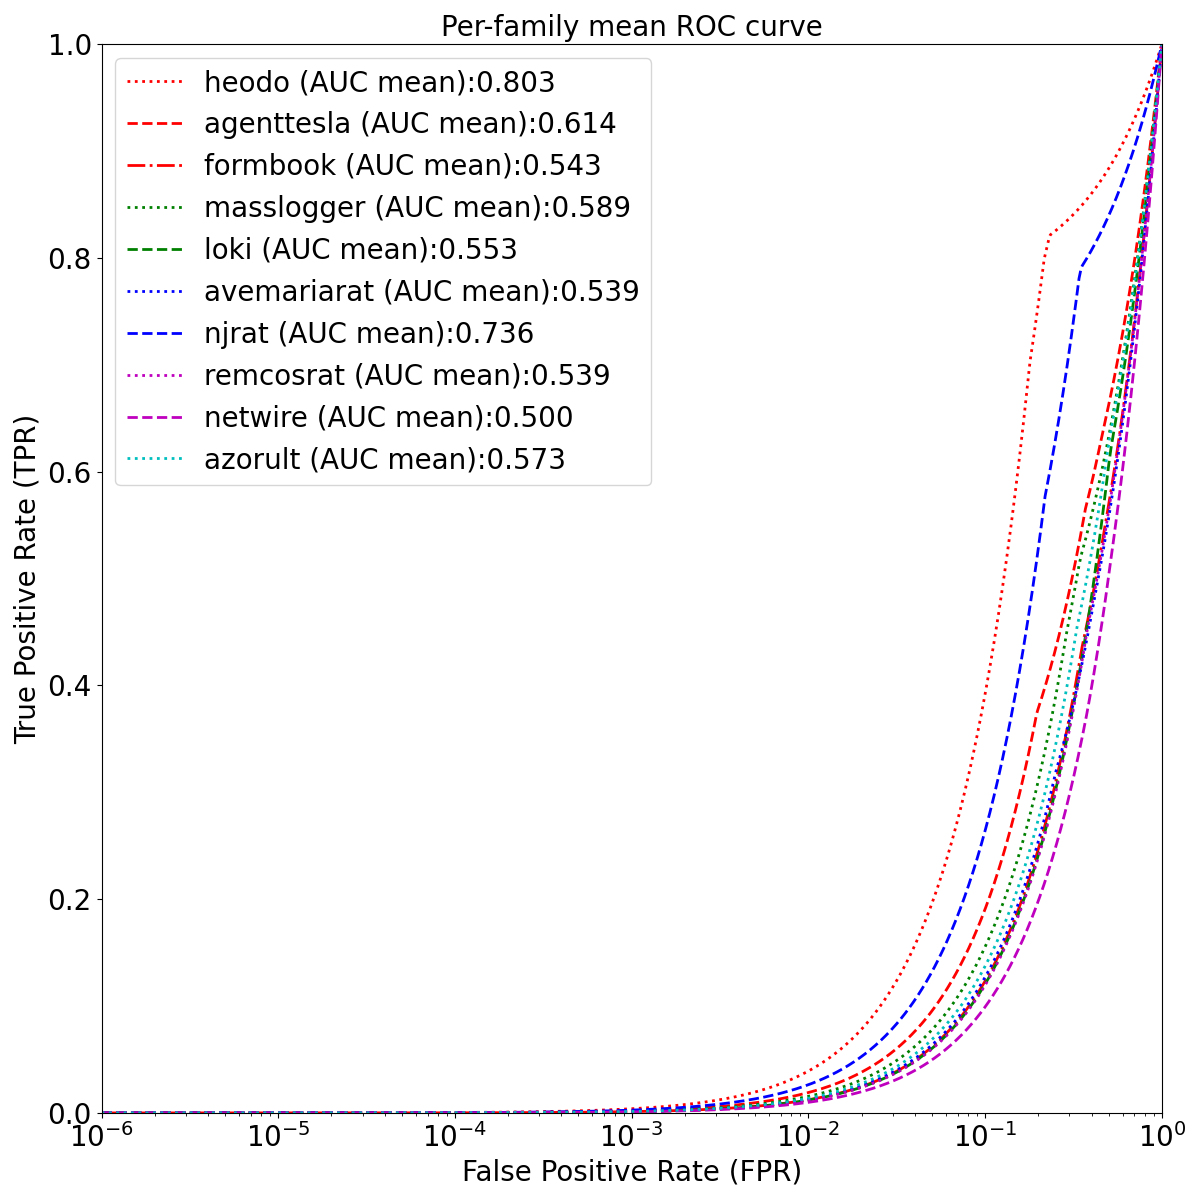
\includegraphics[width=0.6\textwidth]{./results/all_mean_fresh_roc_proposedModel.png}
        \vspace*{-0.2cm}
        \caption{Mean ROC curve and AUC statistics of \textBF{Proposed Model} for the prediction of all families on fresh dataset samples. The line represents the \textit{mean} TPR at a given FPR. Statistics were computed over \textBF{3} training runs, each with random parameter initialization.}
        \label{fig:allMeanFreshRocProposedModel}
    \end{figure}
}
\newcommand{\FamilyClassifierAccuracyResultsTable}{
    \begin{table}[H]
        \centering
        \begin{tabular}{|P{2cm}||P{3,2cm} P{3,2cm} P{3,2cm}|}
            \hline
            & Family Classifier on Joint Embedding & Family Classifier on MTJE Model & Family Classifier only \\
            \hline
            Accuracy & 0.445$\pm$0.005 & \textBF{0.465$\pm$0.003} & 0.414$\pm$0.007 \\
            \hline
        \end{tabular}
        \caption[Family Classifier Accuracy Results]{Mean and Standard deviation of the Family Classifier accuracy obtained by evaluating the Family Classifiers built on top of the \textBF{Joint Embedding} and \textBF{MTJE} model implementations along with a Family Classifier model with no Transfer Learning applied (\textBF{Family Classifier Only}). Results were aggregated over \textBF{3} training runs with different weight initializations and minibatch orderings. Best results are shown in \textbf{bold}.} \label{tab:FamilyClassifierAccuracyResults}
    \end{table}
}

\newcommand{\FamilyClassifierScoresTable}{
    \begin{table}[H]
        \centering
        \begin{tabular}{|P{1,8cm}|P{1,3cm}||P{3cm} P{3cm} P{3cm}|}
            \hline
            & & Family Classifier on Joint Embedding & Family Classifier on MTJE Model & Family Classifier only \\
            \hline
            \multirow{3}{4em}{Jaccard Similarity} & Micro & 0.286$\pm$0.004 & \textBF{0.303$\pm$0.002} & 0.261$\pm$0.006 \\
            & Macro & 0.318$\pm$0.001 & \textBF{0.339$\pm$0.002} & 0.282$\pm$0.011 \\
            & Weighted & 0.318$\pm$0.001 & \textBF{0.339$\pm$0.002} & 0.282$\pm$0.011 \\
            \hline
            \multirow{3}{4em}{Recall} & Micro & 0.445$\pm$0.005 & \textBF{0.465$\pm$0.003} & 0.414$\pm$0.007 \\
            & Macro & 0.445$\pm$0.005 & \textBF{0.465$\pm$0.003} & 0.413$\pm$0.008 \\
            & Weighted & 0.445$\pm$0.005 & \textBF{0.465$\pm$0.003} & 0.414$\pm$0.007 \\
            \hline
            \multirow{3}{4em}{Precision} & Micro & 0.445$\pm$0.005 & \textBF{0.465$\pm$0.003} & 0.414$\pm$0.007 \\
            & Macro & 0.507$\pm$0.001 & \textBF{0.538$\pm$0.006} & 0.473$\pm$0.009 \\
            & Weighted & 0.507$\pm$0.001 & \textBF{0.538$\pm$0.006} & 0.473$\pm$0.009 \\
            \hline
            \multirow{3}{4em}{F1-score} & Micro & 0.445$\pm$0.005 & \textBF{0.465$\pm$0.003} & 0.413$\pm$0.008 \\
            & Macro & 0.438$\pm$0.003 & \textBF{0.460$\pm$0.005} & 0.397$\pm$0.010 \\
            & Weighted & 0.438$\pm$0.003 & \textBF{0.460$\pm$0.005} & 0.397$\pm$0.010 \\
            \hline
            \multirow{3}{4em}{AUC ROC OVO} & Micro & - & - & - \\
            & Macro & 0.815$\pm$0.004 & \textBF{0.830$\pm$0.002} & 0.800$\pm$0.012 \\
            & Weighted & 0.815$\pm$0.004 & \textBF{0.830$\pm$0.002} & 0.800$\pm$0.012 \\
            \hline
            \multirow{3}{4em}{AUC ROC OVR} & Micro & - & - & - \\
            & Macro & 0.815$\pm$0.004 & \textBF{0.830$\pm$0.002} & 0.800$\pm$0.012 \\
            & Weighted & 0.815$\pm$0.004 & \textBF{0.830$\pm$0.002} & 0.800$\pm$0.015 \\
            \hline
        \end{tabular}
        \caption[Family Classifier Scores]{Mean and Standard deviation of the Family Classifier scores obtained by evaluating the Family Classifiers built on top of the \textBF{Joint Embedding} and \textBF{MTJE} model implementations along with a Family Classifier model with no Transfer Learning applied (\textBF{Family Classifier Only}). Results were aggregated over \textBF{3} training runs with different weight initializations and minibatch orderings. Best results are shown in \textbf{bold}.} \label{tab:FamilyClassifierScoresTable}
    \end{table}
}

\newcommand{\FamilyClassifierJointEmbeddingConfusionMatrix}{
    \begin{figure}[H]
        \vspace*{-0.5cm}
        \centering
        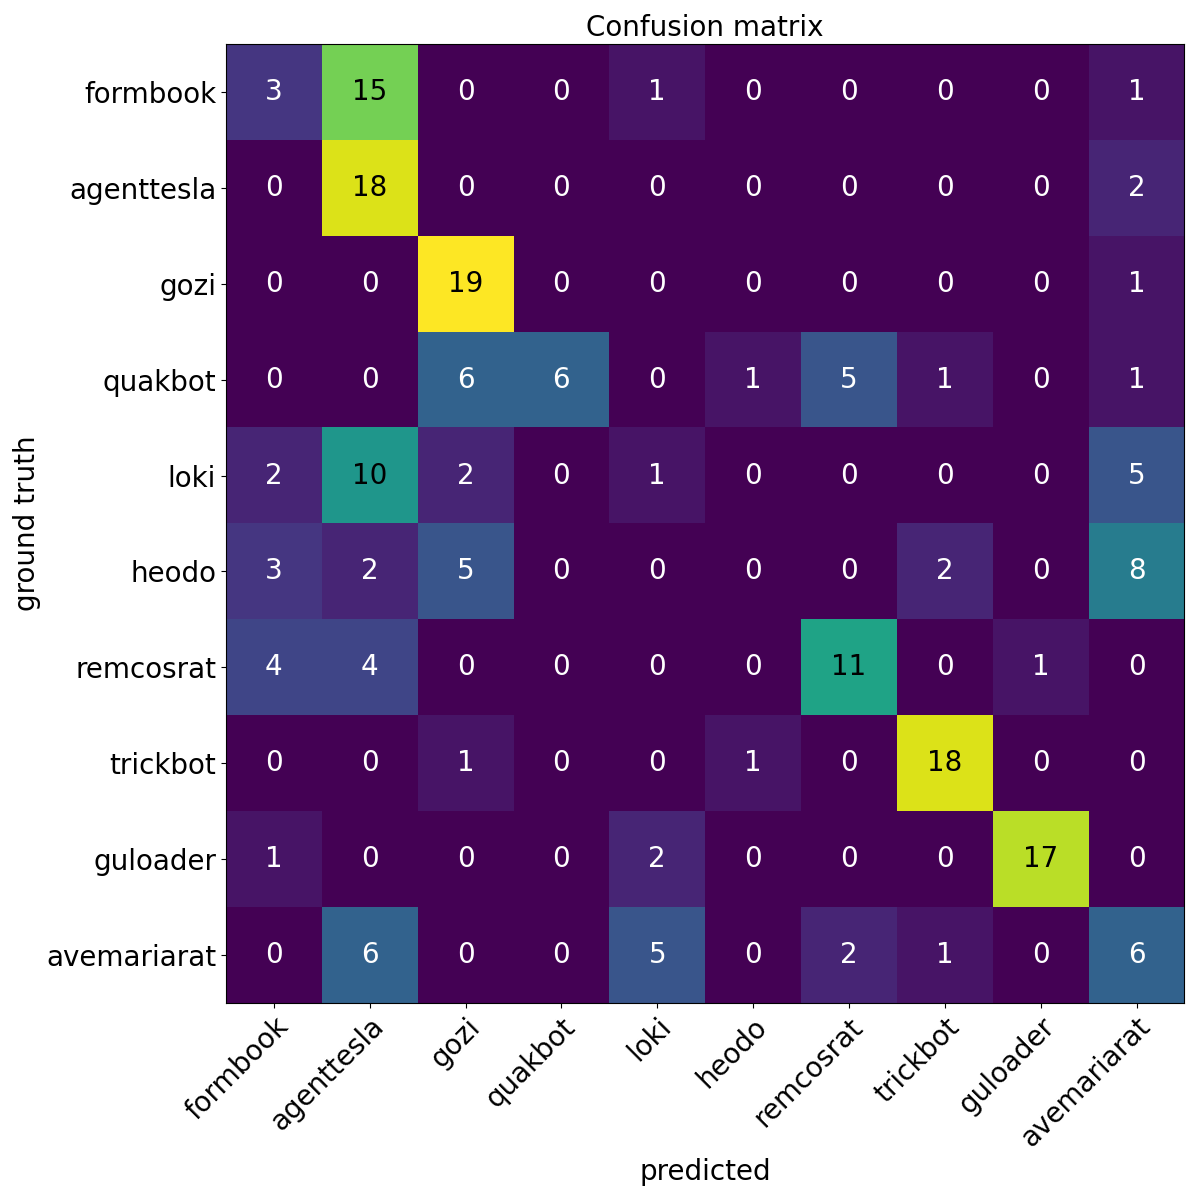
\includegraphics[width=0.7\textwidth]{./results/family_classifier_confusion_matrix_jointEmbedding.png}
        \vspace*{-0.2cm}
        \caption[Family Classifier Joint Embedding Confusion Matrix]{Confusion Matrix resulting from the evaluation of the Family Classifier built on top of the \textbf{Joint Embedding} model implementation.}
        \label{fig:FamilyClassifierJointEmbeddingConfusionMatrix}
    \end{figure}
}

\newcommand{\FamilyClassifierMtjeConfusionMatrix}{
    \begin{figure}[H]
        \vspace*{-0.5cm}
        \centering
        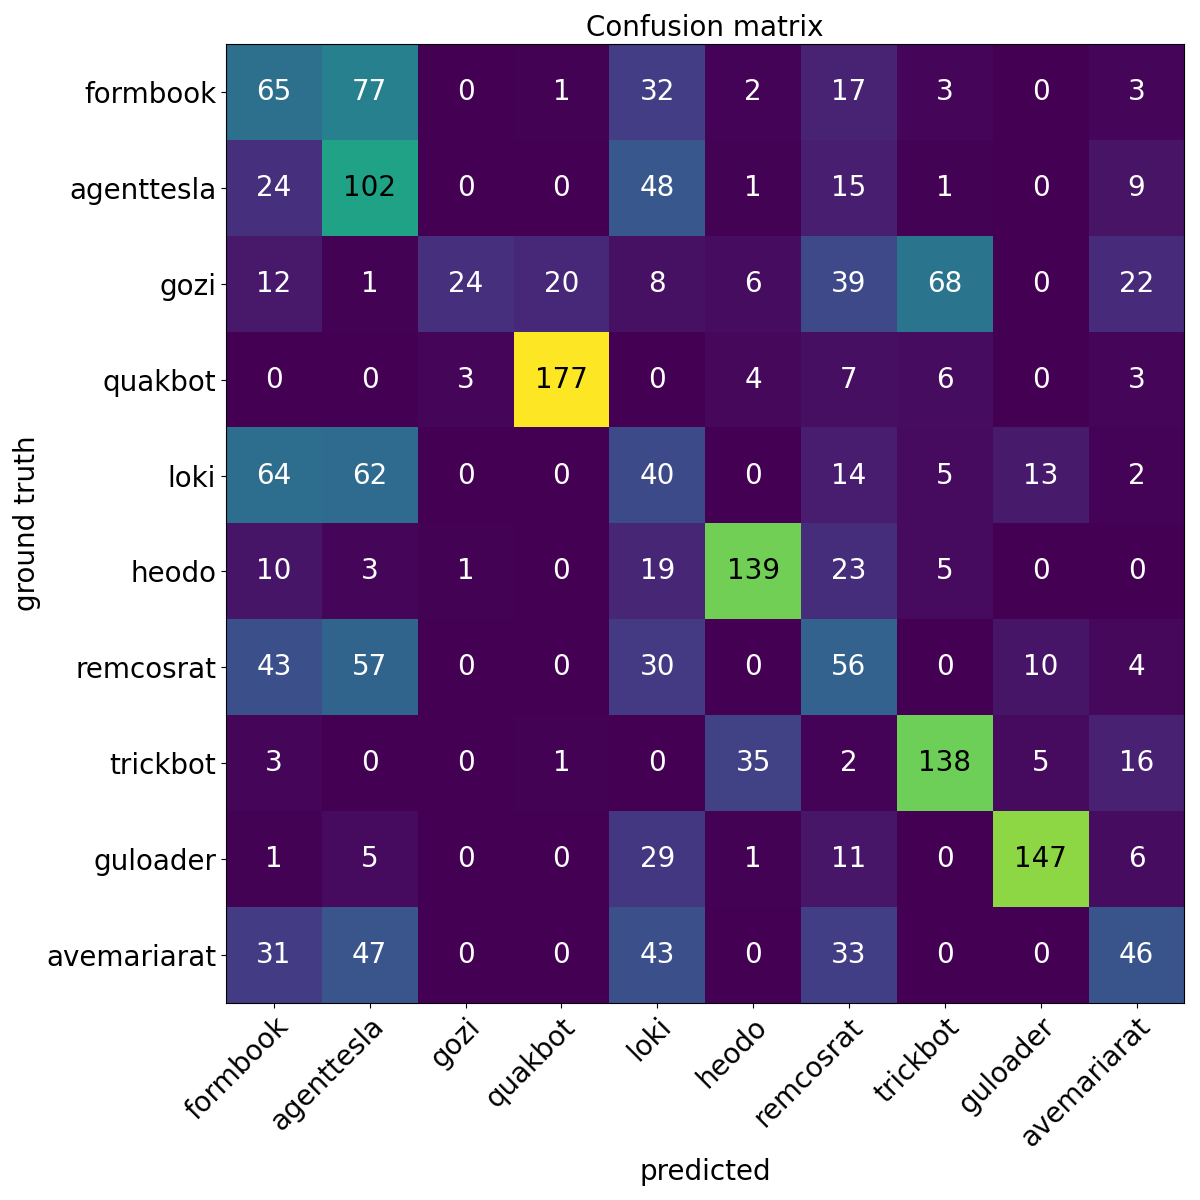
\includegraphics[width=0.7\textwidth]{./results/family_classifier_confusion_matrix_mtje.png}
        \vspace*{-0.2cm}
        \caption[Family Classifier MTJE Model Confusion Matrix]{Confusion Matrix resulting from the evaluation of the Family Classifier built on top of the \textbf{MTJE} Model implementation.}
        \label{fig:FamilyClassifierMtjeConfusionMatrix}
    \end{figure}
}

\newcommand{\FamilyClassifierOnlyConfusionMatrix}{
    \begin{figure}[H]
        \vspace*{-0.5cm}
        \centering
        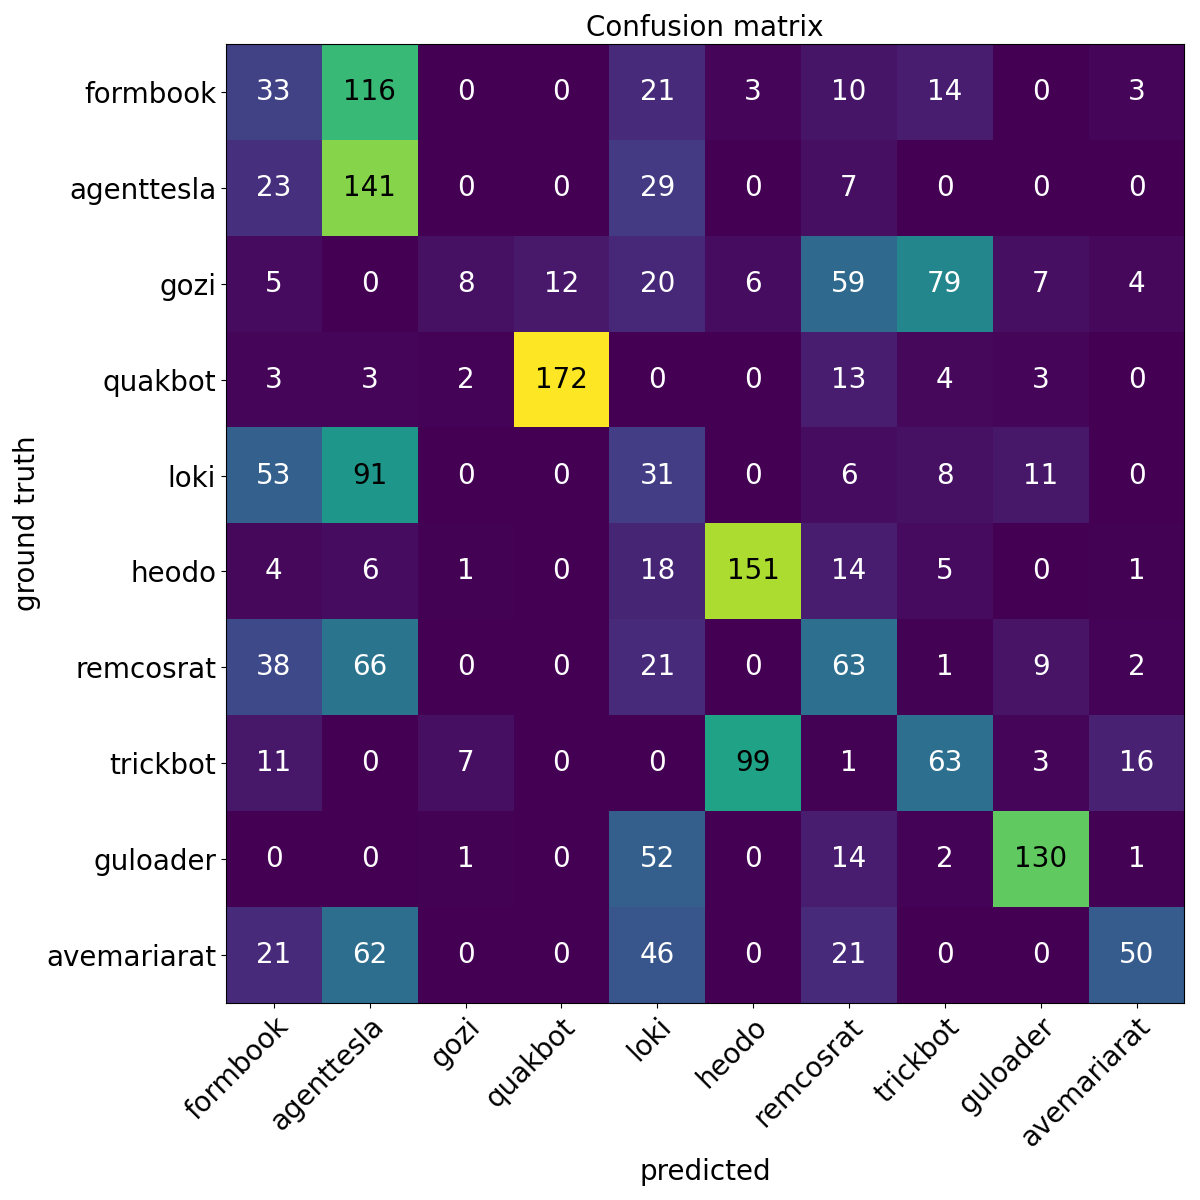
\includegraphics[width=0.7\textwidth]{./results/family_classifier_confusion_matrix_familyClassifierOnly.png}
        \vspace*{-0.2cm}
        \caption[Family Classifier Only Joint Embedding Confusion Matrix]{Confusion Matrix resulting from the evaluation of the \textbf{Family Classifier Only} Model implementation (with no transfer learning).}
        \label{fig:FamilyClassifierOnlyConfusionMatrix}
    \end{figure}
}

\definecolor{codegreen}{rgb}{0,0.6,0}
\definecolor{codegray}{rgb}{0.5,0.5,0.5}
\definecolor{codepurple}{rgb}{0.58,0,0.82}
\definecolor{backcolour}{rgb}{0.95,0.95,0.92}

\lstdefinestyle{mystyle}{
	backgroundcolor=\color{backcolour},   
	commentstyle=\color{codegreen},
	keywordstyle=\color{blue},
	numberstyle=\tiny\color{codegray},
	stringstyle=\color{codepurple},
	basicstyle=\ttfamily\footnotesize,
	breakatwhitespace=false,         
	breaklines=true,                 
	captionpos=b,                    
	keepspaces=true,                 
	numbers=left,                    
	numbersep=5pt,                  
	showspaces=false,                
	showstringspaces=false,
	showtabs=false,                  
	tabsize=2
}

\lstdefinelanguage{YARA}{
	morekeywords=[1]{rule, meta, strings, condition},
	morekeywords=[2]{import, ascii, wide, nocase, and, or, all, at, in, of, fullword},
	keywordstyle=[1]\color{Blue},
	keywordstyle=[2]\color{Red},
	sensitive=false,
	morecomment=[l]{//},
	morecomment=[s]{/*}{*/},
	morestring=[b]",
	morestring=[d]',
}

\newcolumntype{P}[1]{>{\centering\arraybackslash}p{#1}}
\renewcommand{\arraystretch}{1.5}

\newsavebox\CBox
\def\textBF#1{\sbox\CBox{#1}\resizebox{\wd\CBox}{\ht\CBox}{\textbf{#1}}}

\algdef{SE}% flags used internally to indicate we're defining a new block statement
[CLASS]% new block type
{Class}% "\Class{name}" will indicate the start of the class declaration
{EndClass}% "\EndClass" ends the block indent
[1]% There is one argument, which is the name of the class
{\textbf{class} \textsc{#1}}% typesetting of the start of a class
{\textbf{end class}}% typesetting the end of the class

\DeclareMathOperator*{\argmax}{arg\,max}
\DeclareMathOperator*{\argmin}{arg\,min}

\begin{document}
	
\selectlanguage{english}

\ateneo{Politecnico di Torino}

%%% scegliere la propria facolt� (solo PRIMA dell'AA 2012-2013)
%
%\facolta[III]{Ingegneria dell'Informazione}
%\facolta[IV]{Organizzazione d'Impresa\\e Ingegneria Gestionale}
%\Materia{Remote sensing}% uso sconsigliato

%\monografia{Gestione informatizzata di un magazzino ricambi}% per la laurea triennale
\titolo{Automatic Malware Signature Generation}% per la laurea quinquennale e il dottorato
%\sottotitolo{Metodo dei satelliti medicei}% NON obbligatorio, per la laurea quinquennale e il dottorato

%%% scegliere il proprio corso
%
%\corsodilaurea{Ingegneria dell'Organizzazione d'Impresa}% per la laurea di primo e secondo livello
%\corsodilaurea{Ingegneria Logistica e della Produzione}% per la laurea di primo e secondo livello
%\corsodilaurea{Ingegneria Gestionale}% per la laurea di primo e secondo livello
\corsodilaurea{Ingegneria Informatica}% per la laurea di primo e secondo livello
%\corsodidottorato{Meccanica}% per il dottorato

\candidato{Michele \textsc{Crepaldi}}% per tutti i percorsi
%\secondocandidato{Evangelista \textsc{Torricelli}}% per la laurea magistrale solamente
%\direttore{prof. Albert Einstein}% per il dottorato
%\coordinatore{prof. Albert Einstein}% per il dottorato
\relatore{prof.\ Antonio Lioy}% per la laurea e il dottorato
\secondorelatore{ing.~Andrea Atzeni}% per la laurea magistrale
%\terzorelatore{{\tabular{@{}l}dott.\ Neil Armstrong\\prof. Maria Rossi\endtabular}}% per la laurea magistrale
%\tutore{ing.~Andrea Atzeni}% per il dottorato
%\tutoreaziendale{dott.\ ing.\ Giovanni Giacosa} % solo per la laurea di secondo livello con tesi svolta in azienda
%\NomeTutoreAziendale{Supervisore aziendale\\Centro Ricerche FIAT}
%\sedutadilaurea{Agosto 1615}% per la laurea quinquennale
%\esamedidottorato{Novembre 1610}% per il dottorato
%\sedutadilaurea{\textsc{Novembre} 2017}% per la laurea triennale
\sedutadilaurea{\textsc{Anno~accademico} 2020-2021}% per la laurea magistrale
%\annoaccademico{1615-1616}% solo con l'opzione classica
%\annoaccademico{2006-2007}% idem
%\ciclodidottorato{XV}% per il dottorato
\logosede{logopolito}
%
%\chapterbib %solo per vedere che cosa succede; e' preferibile comporre una sola bibliografia
%\AdvisorName{Supervisors}
%\newtheorem{osservazione}{Osservazione}% Standard LaTeX

%\usepackage[a-1b]{pdfx}
%\hypersetup{%
%    pdfpagemode={UseOutlines},
%    bookmarksopen,
%    pdfstartview={FitH},
%    colorlinks,
%    linkcolor={blue},
%    citecolor={green},
%    urlcolor={blue}
%  }

%
% per numerare e far comparire nell'indice anche le sezioni di quarto livello
% SCONSIGLIATO! da usarsi solo in caso di estrema necessit�
%\setcounter{secnumdepth}{4}% section-numbering-depth
%\setcounter{tocdepth}{4}% TOC-numbering-depth (TOC=Table-Of-Content)

%\setbindingcorrection{3mm}

\errorcontextlines=9

\frontespizio
\paginavuota
\newpage
%per sfruttare meglio lo spazio nella pagina
\advance\voffset -5mm
\advance\textheight 30mm

% opzionale, solo se si vuole dedicare la tesi a delle persone care
%\begin{dedica}
%\end{dedica}

\ringraziamenti
I would like to express my sincere gratitude to Professor Antonio Lioy and Ing. Andrea Atzeni for the opportunity they gave me of working on this thesis and for their assistance at every stage of the research project.

I would like to extend my sincere thanks to Ing. Andrea Marcelli for the technical support he offered me and for his insightful comments and suggestions.

Special thanks to my uncle Davide who read the various versions of this thesis, gave me many helpful tips and helped me to define the final document structure and correct grammatical errors.

My most important thanks go to my family to whom I am deeply grateful.\newline
In particular I would like to thank my parents for their unwavering support and trust in me, for how they raised me and for the sacrifices they made for me to reach this goal. I hope to make you proud of me and to repay you for the love you have given me over the years.

I would also like to thank my sister Ilaria, my grandparents, my uncles and my cousins for always being there for me, no matter the circumstances. I'm proud to be part of this family.

I would also like to make a special thanks to my beloved Giulia who has always believed in me and has never failed to cheer me up and make me happy even in the most stressful and difficult days. I hope I can repay you with the same support you gave me on this journey.

Finally, I would like to thank my dearest friends who kept me company during my studies, alleviating the resulting tiredness and tension, despite having made different choices and taken separate paths.

%% inserire sempre nella tesi per la laurea di I livello, perch� il nome dei tutori non � indicato sul frontespizio.
%Il lavoro descritto in questa monografia � stato svolto sotto la supervisione
%del Prof. Antonio Lioy (tutore accademico)% inserire sempre il nome del tutore accademico
% e dell'Ing. Mario Rossi (tutore aziendale)% inserire solo se la monografia � relativa ad un tirocinio.
%.

\sommario
In most recent years the proliferation of malicious software, namely Malware, has had a massive increase: according to AV Atlas Dashboard \cite{AvAtlas} the new malware samples (and PUA - Potentially Unwanted Application) currently detected every day are about 440.000 (at the time of writing), and this number is predicted to only keep growing. The total number of known Microsoft Windows malicious software (and PUA) passed from about 55 million in 2011, to about 400 million in 2016, and finally to nearly 830 million now. The huge number of malware samples out there in the wild renders the detection through manually generated signatures (patterns that identify malicious code) infeasible and consequently imposes the urgent need for tools able to automatically detect malware and possibly describe it in a human-interpretable way. Several methodologies have been proposed through the years, ranging from signature-based detection (especially with Yara Rules) to various Machine Learning approaches like Decision Trees, Naive Bayes models and Neural Networks.

This thesis presents a novel model built upon previous works in \textbf{ML-based} (Machine Learning) automatic PE (Microsoft Windows Portable Executable) malware detection and description and introduces a new evaluation procedure on the learned implicit representation/signature of malware samples that may prove the applicability of its usage in the Malicious family prediction and ranking tasks. The model is trained on an open source large scale dataset of malware and benignware samples with the aim of creating high quality implicit signatures capable of correctly detecting (and describing) unseen malware samples as well as obfuscated malware and new variants, with high True Positive Rate (TPR) and high Recall at low False Positive Rates (FPRs).

The \textbf{Proposed Model}'s results in the different tasks (both the ones it was trained on - Malicious/Benign label and descriptive tags prediction - and the additional malware family prediction and ranking tasks) were compared to the previous models' ones. In particular, the \textbf{ALOHA} model proposed in work \cite{ruddALOHA} and the \textbf{Joint Embedding} model described in paper \cite{DucauAMDATSE} were selected as reference models.

The results show that the \textbf{Proposed Model} generates implicit signatures (samples embeddings) which provide higher TPRs, Accuracies, Recalls, Precisions and F1 Scores at low false positive rates with respect to the ones produced by the mentioned previous methods on the corresponding tasks. When testing the \textbf{Proposed Model}'s learned representations on the Malware Family prediction and ranking tasks, however, the results were less promising. Therefore, a new Malware \textbf{Family Classifier} model, built on top of the \textbf{Proposed Model} base topology, was created. This new model was trained and evaluated on the malware family classification task using a specially crafted dataset of $10.000$ PE files, exploiting the parameters from a previous \textbf{Proposed Model} training run, with the aid of transfer learning. The introduction of this new Family Classifier provided more meaningful results, although not exceptional, in the family classification task while also demonstrating the potential of using Transfer learning in this context.

Future (and more performant) works capable of overcoming some of the final model limitations may be very useful to the IT-Security field in the current scenario and could even enable the generation of explicit (and thus more interpretable) signatures derived from the learned implicit ones.

%\tablespagetrue % normalmente questa riga non serve ed e' commentata
%\figurespagetrue % normalmente questa riga non serve ed e' commentata

\indici

\mainmatter

\chapter{Introduction}
Malware first made its appearance in the 1960s. Then, hackers used to design computer viruses mainly for fun, as an exciting prank/experiment; their creations would generally display harmless messages and then spread to other computers \cite{ReganWIM}. There are numerous examples of malware created at that time within a laboratory setting: for example the \textbf{\textit{Darwin game}} in 1962 and \textbf{\textit{Creeper}} in 1971.

In the early 1980s, the concept of malware caught on in the technology industry, and numerous examples of viruses and worms appeared both on Apple and IBM personal computers. With the introduction of the World Wide Web and the commercial internet in the 1990s it eventually became widely popularized, so much that Yisreal Radai coined the term \textbf{malware} in 1990.

\begin{figure}[h!]
	\centering
	\includegraphics[width=0.6\textwidth]{./images/elk_cloner_example.png}
	\caption[Poem displayed by Elk Cloner virus]{Poem displayed by Elk Cloner virus}
	\label{fig:elkClonerExample}
\end{figure}

The previously mentioned 1960s and 1970s malware were all kept within a laboratory environment and never managed to escape to the wild. \textbf{\textit{Elk Cloner}} (1981) was the first known virus to have been able to escape its creation environment. It spread through infected floppy disks but did not cause deliberate harm simply displaying the 'poem' shown in figure \ref{fig:elkClonerExample} on the user's screen. Following the success of that prank gone wild, the first Microsoft PC virus, called \textbf{\textit{Brain}}, was then created in 1986. Again, like \textit{Elk Cloner}, Brain was mostly annoying rather than harmful, but it was also the first known virus capable of concealing its presence on the disk thus evading detection. In 1988 the first worm, called \textbf{\textit{Morris}} worm, an experimental, self-propagating, self-replicating program was released on the internet \cite{NamanyaTWM}. In 1988 made its appearance also the first example of intentionally harmful virus, the \textbf{\textit{Vienna}} virus, which encrypted data and destroyed files. This led to the creation of the first antivirus tool ever \cite{ReganWIM}.

In the following decades malware has evolved both regarding its complexity and malware sample numbers. In particular, according to AV Atlas \cite{AvAtlas}, in 2019 and 2020 (and until mid 2021 - that is until the time of writing) the number of newly generated malware blew with respect to previous years, as shown in graph \ref{fig:avAtlasReportNew}, to the point that approximately 5.1 new Microsoft Windows malware (and PUA) are currently generated per second, $\sim18,500$ per hour. As reported by AV Atlas dashboard and as shown in graph \ref{fig:avAtlasReport}, in recent years the total amount of unique malware (and PUA) variants reached impressive numbers, to the point that they are now more than $830$ millions. Moreover, nowadays malware commonly use obfuscation and other sophisticated techniques, such as Polymorphism and Metamorphism, to evolve their structure thus evading detection.

\begin{figure}[H]
	\includegraphics[width=\textwidth]{./images/av_atlas_report_total_amount_new.png}
	\caption[AV Atlas - Total Amount of New Malware and PUA]{AV Atlas - Total Amount of New Malware and PUA}
	\label{fig:avAtlasReportNew}
\end{figure}

\begin{figure}[H]
	\includegraphics[width=\textwidth]{./images/av_atlas_report_total_amount.png}
	\caption[AV Atlas - Total Amount of Malware and PUA]{AV Atlas - Total Amount of Malware and PUA}
	\label{fig:avAtlasReport}
\end{figure}

For all these reasons, signature-based detection techniques (such as manually generated Yara Rules), which are typically used by most commercial anti-virus solutions, are becoming inefficient in the present scenario. In fact, it is now straight up impossible for analysts to manually analyse each malware variant that is found in the wild. Moreover, even when a new malware family is identified and an appropriate amount of its samples are analysed, the generated signature may not be capable of detecting new variations or may even be rendered useless through the use of obfuscation and/or polymorphic mechanisms. There is therefore the need for automated malware analysis solutions capable of automatically generating (implicit or explicit) signatures effective at distinguishing malicious from benign code while being less susceptible to code modifications and obfuscation attempts.

This thesis presents a research aimed at satisfying this need for automated malware detection solutions. In particular, it presents a novel model built upon previous works on ML-based (Machine Learning) automatic malware detection and description designed for PE (Microsoft Windows Portable Executable) files. Moreover, it introduces a new evaluation procedure that may prove the applicability of the model learned implicit representation/signature of malware samples in the Malware family prediction and ranking tasks. These tasks are particularly interesting for malware analysts since they allow them to quickly categorize malware samples as being part of specific sets (families) of samples with common behavioural and structural characteristics.

The proposed framework life cycle can be conceptually divided in four phases (as shown in figure \ref{fig:frameworkLifecycle}): \textbf{model architecture definition}, \textbf{model training and validation}, \textbf{model evaluation} and finally \textbf{model deployment}. In particular, in the first phase the proposed FNN (Feedforward Neural Network) model architecture is defined and implemented taking inspiration from previous works such as the \textbf{ALOHA} and the \textbf{Joint Embedding} models presented in papers \cite{ruddALOHA} and \cite{DucauAMDATSE}, respectively. In the second phase, instead, the proposed model is trained (and validated) on an open source large scale dataset of malware and benignware samples (Sorel20M \cite{HarangSOREL20M}) with the aim of creating high quality implicit signatures capable of detecting (and describing via SMART tags) unseen malware samples, as well as obfuscated malware and new variants, with high True Positive Rate (TPR) and high Recall at low False Positive Rates (FPRs). The first two phases here described are iteratively repeated until a model with satisfactory training and validation loss trends is generated. In the third phase, on the other hand, the final model architecture is tested on the Malware detection and Description tasks and the corresponding prediction scores are computed and plotted. Moreover, in this phase the model learned representation of PE files is also tested on the Malware family prediction and ranking tasks using a novel dataset, referred to as '\textit{fresh dataset}' in this document, containing $10.000$ samples belonging to $10$ of the most widespread malware families in Italy at the time of writing, specifically created for that purpose. In both datasets the samples are directly represented by their numerical feature representation extracted statically from specific fields of each sample's Windows Portable Executable (PE) file header. The proposed model thus relies exclusively on static analysis features which are generally simpler, less computationally intensive and thus faster than dynamic analysis ones (executable's behaviour characteristics). Finally, in the last phase the final proposed model architecture is deployed in the wild. In particular, it can be used as an automatic Malware detection tool that provides additional description tags useful for remediation. Moreover, potentially, if the corresponding evaluation results allow it, it could also be used to provide information about the malware family each analysed sample most probably belongs to, among the set of families of interest.

\begin{figure}[H]
	\centering
	\includegraphics[width=0.9\textwidth]{./images/framework_lifecycle.png}
	\caption[Proposed Framework Life Cycle]{Proposed Framework Life Cycle}
	\label{fig:frameworkLifecycle}
\end{figure}

This thesis focuses on the first three phases previously mentioned. In particular, it concentrates on defining, training and evaluating the best model architecture possible for the tasks at hand. However, some code optimization challenges resulting from the slowness of the code in the instance used for the experiments meant that it could be possible to train the model only with the first half of the samples of the Sorel20M dataset in a reasonable time, with some approximations on the samples dispersion when random sampling them from the dataset. This led to slightly worse performance than what is theoretically possible with the current architecture using the whole dataset. Nevertheless, the deployment of the proposed model on a real-world scenario is theoretically possible with the current final architecture, although it would be better to train the proposed model on the whole Sorel20M dataset on a better instance first in order to see its true potential.

At a later moment, the proposed framework was extended with the addition of a \textbf{Malware Family Classifier} model head defined on top of the \textbf{Proposed Model} base topology in order to improve its relatively poor results in the Malware Family Prediction task. This new model was then specifically trained (and tested) for such purpose on the relatively small '\textit{fresh dataset}', which contains information about the malware family each sample belongs to. However, instead of training the newly defined architecture from scratch on such small dataset at the risk of overfitting, the technique called '\textit{Transfer Learning}' was used by transferring the knowledge (the learned model parameters) from a previous \textbf{Proposed Model} training run on the large Sorel20M dataset onto the new model base topology (the one shared with the \textbf{Proposed Model} architecture), before training. Then, during the training procedure some of the imported parameters were 'fine-tuned' while the ones corresponding to the newly added Family Classifier head were learned from scratch.

\chapter{Background}

\section{Malware}
\textbf{Malware}, short for \textbf{\textit{malicious software}}, is a general term for all types of programs designed to perform harmful or undesirable actions on a system. In fact in the context of IT security the term \textit{malicious software} commonly means \cite{SharpAIM}:

\begin{quote}
	\textit{"Software which is used with the aim of attempting to breach a computer system's security policy with respect to Confidentiality, Integrity and/or Availability."}
\end{quote}

Malware consists of programming artefacts (code, scripts, active content, and other software) designed to disrupt or deny operation, gain unauthorized access to system resources, gather information that leads to loss of privacy or exploitation, and other abusive behaviour.
Malware is not (and should not be confused with) defective software - software that has a legitimate purpose but contains harmful bugs (programming errors).

Different companies, organizations and people describe malware in various ways. For example \textbf{Microsoft} defines it in a generic way:

\begin{quote}
	\textit{"Malware is a catch-all term to refer to any software designed to cause damage to a single computer, server, or computer network"} \cite{MoirDM}.
\end{quote}

The \textbf{National Institute of Standards and Technology} (\textbf{NIST}), on the other hand, presents multiple definitions for malware, describing it as "hardware, firmware, or software that is intentionally included or inserted in a system for a harmful purpose" \cite{nistM}.

In another more specific definition \textbf{NIST} affirms that Malware is:

\begin{quote}
	\textit{"A program that is inserted into a system, usually covertly, with the intent of compromising the confidentiality, integrity, or availability of the victim's data, applications, or operating system or of otherwise annoying or disrupting the victim"} \cite{nistM}.
\end{quote}

The computer system whose security policy is attempted to be breached is usually known as the \textbf{\textit{target}} for the malware. The cybercriminal who originally launched the malware with the purpose of attacking one or more targets, on the other hand, is generally referred to as the "\textit{initiator} of the malware". Furthermore, depending on the malware type, the initiator may or may not exactly know what the set of targets is \cite{SharpAIM}.

According to the above definitions software is defined as malicious in relation to an attempted breach of the target's \textbf{\textit{security policy}}.
In other words, software is often identified as malware based on its \textit{intended use}, rather than the particular technique or technology used to build it.

\subsection{Why is Malware used}
Generally, cybercriminals use malware to access targets' sensitive data, extort ransoms, or simply cause as much damage as possible to the affected systems.

More generally malware serves a variety of purposes. For example, the most common cybercriminals' uses of malware are: \cite{CraneWIM}

\begin{itemize}
	\item \textbf{To profit financially (either directly or through the sale of their products or services)}.
	For example, attackers may use malware to infect targets' devices with the purpose of stealing their credit account information or cryptocurrency. Alternatively, they may sell their malware to other cybercriminals or as a service offering (\textit{malware-as-a-service}).
	
	\item \textbf{As a means of revenge or to carry out a personal agenda}.
	For example, Brian Krebs of Krebs on Security was struck by a big DDoS attack in 2016 after having talked about a DDoS attacker on his blog.
	
	\item \textbf{To carry out a political or social agenda}.
	For example, there exist many Nation-state actors (such as state-run hacker groups in China and North Korea) and hacker groups such as Anonymous.
	
	\item \textbf{As a way to entertain themselves}.
	Some cybercriminals perpetrate attacks on victims just for fun.
\end{itemize}

Obviously there are also reasons for \textbf{non}-malicious actors to create and/or deploy some types of malware too - for example they can be used to test a system's security, to spy on someone as part of a legal act/police operation, etc.

\subsection{Common Malware types}
There are different ways of categorizing malware; one way is by \textit{how} the malicious software spreads. Another one is by \textit{what} it \textit{does} once it has successfully infected its victim's computers (i.e. what is its payload, how it exploits the system or makes it vulnerable).

\subsubsection{By how they spread}
Terms like \textit{trojan}, \textit{virus} and \textit{worm} are commonly used interchangeably to indicate generic malware, but they actually describe three subtly different ways malicious software can infect target computers \cite{SymantecDVWT}:

\begin{itemize}
	\item \textbf{\textit{Trojan horse}}. Generally speaking, a \textit{Trojan Horse}, commonly referred to as a "Trojan", is any program that disguises itself as legitimate and invites the user to download and run it, concealing a malicious payload. When executed, the payload - malicious routines - may immediately take effect and cause many undesirable effects, such as deleting the user files or installing additional malware or PUAs (Potentially Unwanted Apps), depending on the payload attached to them \cite{NamanyaTWM}.
	
	Trojans may hide in games, apps, or even software patches, or they may rely on social engineering and be embedded in attachments included in phishing emails. However, they cannot self-replicate but rely on the system operators to activate.
	
	\item \textbf{\textit{Virus}}. The term "computer virus" is used for describing a \textbf{passive} self-replicating malicious program. Usually spread via infected websites, file sharing, or email attachment downloads, it lies dormant until the infected host file or program is activated. At that point it spreads to other executables (and/or boot sectors) by embedding copies of itself into those files. A virus, in fact, in order to spread from one computer to another, usually relies on the infected files possibly ending up, by some means or another, in the target system. The mean of transport (file, media file, network file, etc.) is often referred to as the virus \textit{vector}. Depending on how complex the virus code is, it may be able to modify its copies upon replication. For the transport of the infected files to the target system(s), the virus may rely on an unsuspecting human user (who for example uses a USB drive containing the infected file) or may initiate the transfer itself (for example, it may send the infected files as an e-mail attachment) \cite{SharpAIM}.
	
	Viruses may also perform other harmful actions other than just replicating, such as creating a backdoor for later use, damaging files, stealing information, creating botnets, render advertisements or even damaging equipment.
	
	\item \textbf{\textit{Worm}}. A worm is a self-replicating, \textbf{active} malicious program that exploits various system vulnerabilities to spread over the network. Particularly, it relies on vulnerabilities present in the target's operating system or installed software. Worms usually consume a lot of bandwidth and processing resources due to continuous scanning and may render the host unstable, sometimes even causing crashes. Apart from replicating, computer worms also contain "payloads"  which are pieces of code written to perform various nefarious actions on the affected hosts, for example stealing data, deleting files or creating bots - which can lead the infected systems to become part of a botnet \cite{NamanyaTWM}.
	
\end{itemize}

Moreover, attackers can also install malware "manually" on a computer, either by gaining physical access to the target system or by using privilege escalation methods to obtain remote administrator access \cite{FruhlingerME}.

\subsubsection{By what they do}
There is a wide range of potential attack techniques used by malware, here are briefly described some of them:

\begin{itemize}
	\item \textbf{\textit{Adware}}. \textit{Adware} is any software package which automatically plays, displays, or downloads advertisements to a computer. These can be in the form of pop-up ads, ad banners in websites, or advertisements displayed by software, that lure the user into making a purchase. The goal of Adware is, in fact, to generate revenue for its author.
	
	Often times adware comes even bundled with "free", or discounted, versions of non-malicious software and/or applications since it is usually seen by developers as a way to recover development costs \cite{MullinsMT}.
	
	Adware, by itself, is annoying but somewhat harmless, since it is solely designed to deliver ads; however, it often comes bundled with spyware (such as keyloggers), and/or other privacy-invasive software that is capable of tracking user activity and steal information \cite{DuPaulCMT}.
	
	\item \textbf{\textit{Backdoor}}. A \textit{backdoor}, also called Remote Access Trojan (RAT), is a vulnerability deliberately buried into software's code allowing to bypass typical protection mechanisms, like credentials-based login authentication. Once a system has been compromised (by others types of malware or other methods), one or more backdoors may be installed. This is done with the purpose of allowing the attacker easier access in the future without alerting the user or the system's security programs. Moreover, backdoors may also be installed before other malicious software, to allow attackers entry \cite{MullinsMT}.
	
	On the other hand, it is not uncommon to see many (non-malicious) device or software manufacturers ship their products with intentionally hidden backdoors to allow company personnel or law enforcement access to the system when needed \cite{IngallsTOM}. Alternatively, backdoors are sometimes hidden in programs also by intelligence services.
	
	\item \textbf{\textit{Browser Hijacker}}. A \textit{Browser Hijacker}, also called "hijackware", is a type of malicious program which considerably modifies the behaviour of the victim's web browser. It can be used to make money off unwanted ads, to steal information from users, or to infect the systems with other malware by redirecting users to malicious websites \cite{IngallsTOM}.	
	
	\item \textbf{\textit{Bots}/\textit{Botnet}}. In general, \textit{bots} (short for 'robots') are software programs designed to automatically perform specific operations. Some bots are used for legitimate and harmless purposes such as video programming, video gaming, internet auctions and online contest, among other functions. It is however becoming increasingly common to see bots being used maliciously. Malicious bots can be (and usually are) used to form botnets. A botnet is defined as a network of host computers (zombies/bots) that is controlled by an attacker - the \textit{bot-master} \cite{NamanyaTWM}. Botnets are frequently used for DDoS (Distributed Denial of Service) attacks, but there are other ways that botnets can be useful to cybercriminals: for example they can be employed to carry out brute force attacks on websites or to distribute malware \cite{CraneWIM}.
	
	\item \textbf{\textit{Crypto-miner}}. Crypto-miners are a relatively new malware family. Cybercriminals employ this type of malicious tools to mine Bitcoin and/or other similar digital currencies on the target machine by exploiting the victim system's computing power, without the owner realising it. Obviously, the mined coins end up in the attackers' digital crypto wallets.
	
	Recently, a more modern method of crypto-mining that works within browsers (also called crypto-jacking), has become quite popular \cite{MyraSecurityWIM}.
	
	\item \textbf{\textit{File-less malware}}. As the term suggests, File-less malware is a type of malware that operates from a victim's computer memory, not from files on the hard drive, taking advantage of legitimate code and tools (known as "LOLBins" \cite{CraneWIM}) already existing within the system. File-less malware leaves no malware files to scan and no malicious processes to detect, and is therefore harder to detect and remove than traditional malware: it is, in fact, up to ten times more successful \cite{BakerMCTM}. Furthermore, it also renders forensic analysis more difficult because it disappears from the victim's computer upon rebooting.
	
	\item \textbf{\textit{Keylogger}}. Keyloggers, often considered as being a sub-category of spyware, are malicious programs which secretly track keystrokes on a keyboard, without the system's owner consent - action that is usually referred to as \textit{keylogging} or \textit{Keystroke logging}. The collected data is stored and sent to the attacker who uses it to figure out highly sensitive information such as passwords, usernames and payment details. Keylogging can be performed in various ways, ranging from hardware and software-based approaches to the more sophisticated electromagnetic and acoustic analysis \cite{MullinsMT}.
	
	\item \textbf{\textit{RAM Scraper}}. \textit{RAM scraper} malware, also known as \textit{Point-of-Sale (POS)} malware, targets POS systems like cash registers or vendor portals, harvesting data temporarily stored in RAM (Random Access Memory). Doing so the attacker can easily access unencrypted credit card numbers \cite{IngallsTOM}.
	
	\item \textbf{\textit{Ransomware}}. \textit{Ransomware}, also known as "encryption" or "crypto" Trojan, is a malicious program that, after having infected a host or network, holds the system captive and displays a message requesting a ransom to the host/network users. In particular, it encrypts data on the infected system (or anyway it locks down the system preventing user access) and only unblocks it when the correct password - decryption key - is entered. Without the latter, is practically impossible to regain access to the system. Digital currencies such as Bitcoin and Ether are the most common means of payment, making it difficult to track cybercriminals. Moreover, paying the ransom does not guarantee the user to receive the necessary decryption key. Additionally, some forms of ransomware threaten victims to publicize sensitive information within the encrypted data in order to convince them to pay the ransom.

	\item \textbf{\textit{Rogue Security Software}}. \textit{Rogue Security Software} can be considered as a from of scareware. This type of malware programs presents itself as a security tool to remove risks from the user's system. In reality, this fake security software installs more malware onto the system \cite{IngallsTOM}.
	
	\item \textbf{\textit{Rootkit}}. A \textit{rootkit} is generally thought as a type of malicious software, or a collection of software tools, designed to remotely access or control a computer without being detected by users or security programs. An attacker who has installed a rootkit on a system is able to perform a wide range of malicious activities such as remotely executing files, logging user activities, installing hidden malware, etc. Since a rootkit operates stealthily and continually hides its presence, its prevention, detection and removal can be difficult and often relies manual methods \cite{DuPaulCMT}.
	
	More recently, the term "rootkit" has often been used to refer also to concealment routines in a malicious program. These highly advanced and complex routines are  written to hide malware within legitimate processes on the infected computer. In fact, once a malicious program has been installed on a system, it is essential that it remains hidden, to avoid detection and disinfection \cite{MullinsMT}.

	\item \textbf{\textit{Scareware}}. Scareware is a generic term for malware that uses social engineering to frighten and manipulate users, inducing them into thinking their system is vulnerable or has been compromised. However, in reality no danger has actually been detected: it is a scam. The attack succeeds when the user purchases unwanted - and potentially dangerous - software in an attempt to eliminate the "threat". Generally, the suggested software is additional malware or allegedly protective software with no value whatsoever \cite{MyraSecurityWIM}.

	Some versions of scareware act as a sort of shadow version of ransomware; they claim to have taken control of the victim's system and demand a ransom. However they are actually just trying to fool the victim \cite{FruhlingerME}.
	
	\item \textbf{\textit{Spyware}}. \textit{Spyware}, another name for \textit{privacy-invasive software}, is a type of malicious software that spies on the infected system's user activity. Specifically it can collect various types of personal information about users, such as Internet browsing habits, credit card details and passwords, without their knowledge. The information gathered is then sent back to the responsible cybercriminal(s).
		
	However, the functions of spyware often go far beyond simple activity monitoring and information gathering. In fact, they may also interfere with the user's control of the computer in other ways, such as installing additional software, redirecting web browser activity and changing computer settings \cite{MullinsMT}.
	
	Law enforcement, government agencies and information security organizations often use spyware to monitor communications in a sensitive environment or during an investigation \cite{McAfeeWIM}.
\end{itemize}

\subsubsection{Other cyber-threats}
Other cyber threats which are not strictly, and should not be confused with, malware are, for example:

\begin{itemize}
	\item \textbf{\textit{Software Bug}}. A software bug is an error, or flaw, in a computer program code or system that causes it to produce an incorrect or unexpected result, or to behave in unintended ways. Usually, most of these defects arise from human errors made in the program's source code. Minor bugs only slightly affect the behaviour of a program and can therefore remain undiscovered for quite a long time. On the other hand, more significant bugs can cause crashes or freezes \cite{DuPaulCMT}.
	
	\item \textbf{\textit{Software Vulnerability}}. In computer security, a vulnerability is a hole or a weakness in an application, which can be a design flaw or an implementation bug, that can be exploited by a threat actor, such as an attacker to bypass access controls such as user authentication, override access privileges, steal data or perform other unauthorized actions within a computer system potentially causing harm to the stakeholders of an application. Stakeholders include the application owner, application users, and other entities that rely on the application \cite{OWASPV}.
	
	\item \textbf{\textit{Malvertising}}. Malvertising is the use of legitimate ads or ad networks to covertly deliver malware to unsuspecting users' computers. For example, a cybercriminal might pay to place a malicious ad on a legitimate website. When clicked, it either redirects the victims to a malicious website or installs malware on their computer. In some cases, the code embedded in an ad might even execute automatically without any action from the user, a technique referred to as a "drive-by-download".
	
	\item \textbf{\textit{Phishing}}. Phishing is a type of social engineering attack in which the attacker attempts, through email messages (or other means), to trick users into divulging passwords or other personal and financial information, downloading a malicious attachment or visiting a website that installs malware on their systems.
		
	Some phishing emails are highly sophisticated and can deceive even experienced users, especially if the attacker has successfully compromised a known contact's email account and uses it to spread phishing attacks or malware such as worms. Others are less sophisticated and simply spam as many emails as possible with messages such as "Check your bank account details" \cite{ComtactWDYM}.

	\item \textbf{\textit{Spam}}. In cybersecurity, unsolicited emails are generally referred to as \textit{spam}. Typically, spam includes emails carrying unwanted advertisements, fraud attempts, links to malicious websites or malicious attachments. Most spam emails contain one or more of the following characteristic traits \cite{IngallsTOM}:
	\begin{itemize}
		\item Poor spelling and grammar
		\item Unusual sender address
		\item Unrealistic claims
		\item Suspicious links
	\end{itemize}
\end{itemize}

\subsubsection{General considerations on malware types}
Malware samples are usually categorised both by their means of infection and their behavioural category: for instance, \textit{WannaCry} is a ransomware worm. Moreover, a particular piece of malware may have various forms with different attack vectors: e.g., the banking malware called \textit{Emotet} has been spotted in the wild as both a trojan and a worm \cite{FruhlingerME}. Finally, many instances of malware fit into multiple categories: for example \textit{Stuxnet} is both a worm, a virus and a rootkit.

\section{Detection evasion}
From the creation of the first malwares in 1960s, which were designed by hackers mainly for fun, a strong competition between attackers and defenders has risen. In order to defend from malware attacks, anti-malware groups have been developing increasingly complex (and clever) new techniques. On the other hand, malware developers have conceived and adopted new tactics/methods to avoid the malware detectors \cite{Szor_P}.

The first types of anti-malware tools were mostly based on the assumption that malware structures do not change appreciably during time. In fact, initially, the malware machine code was completely unprotected. This allowed analysts to exploit opcode sequences to recognise specific malware families. Recently, however, a big advancement led to the so-called "second generation" malware \cite{Sharma_2014}, which employs several obfuscation techniques and can create numerous variants of itself, with the purpose of evading such opcode signatures. This posed a challenge to anti-malware developers.

The first malware to exhibit a detection avoidance behaviour was the \textit{Brain} virus \cite{SkoudisFMC}, in 1986. Such malware, in fact, managed to conceal the infected disk section whenever the user attempted to read it, forcing the computer to display clean data instead of the infected part. From that moment on, the ever increasing popularity of detection evasion techniques among malware writers has shown that malware survival in the victim's machine has become of primal importance: the longer the malware remains undetected, the more harm it can do and the more profitable it is to its writer \cite{NamanyaTWM}.

\subsection{Reverse-Engineering}
\textit{Reverse engineering}, in broad terms, indicates the process of extracting knowledge, ideas, design philosophy etc. from anything man-made \cite{EilamRSRE}.

Software reverse engineering is the application of reversing methodologies and techniques to extract knowledge from a software product in order to better understand its inner workings.

Both malicious actors and malware analysts/investigators extensively use reversing techniques, but with opposing purposes. Malware developers often use them to discover vulnerabilities in systems or programs, while analysts and antivirus software developers use them mainly for analysing malicious programs to understand how they work, what damages they can cause, how they infect the system and reproduce and, most importantly, how they can be removed, detected and avoided.

\subsection{Malware analysis}
Malware analysis is the process of extracting as much information as possible from malicious samples discovered in the wild, which usually are in the form of machine code executables (compiled executables), in order to determine their purpose and functionality (and associated threats). This process allows security teams to take a number of useful actions such as: developing effective detection techniques against the analysed malicious code, containing its damage, reversing its effects on the targeted system, developing removal tools that can delete it from infected machines (to cleanly remove a piece of malware from an infected machine it is usually not enough to delete the binary itself) and designing methods to guard systems against future infections \cite{BayerDAMC}.

Initially malware analysts/researchers had to manually analyse each malware sample. This process was however rather complex, it required high expertise, and was quite time-consuming. Moreover, the number of malware samples that nowadays need to be analysed on a daily basis is of the order of hundreds. This implies that the analysis of malware samples can no longer be exclusively done manually. As such, several analysis tools have been developed in recent years to facilitate analysts in analysing malware samples.

Traditionally, there are two main types of analysis: \textit{static} and \textit{dynamic}. Moreover, these two types can be, and frequently are, combined together (\textit{hybrid} analysis) in various stages of malware analysis to optimize results \cite{NamanyaTWM}.

\subsubsection{Static analysis}
\textit{Static analysis} consists of examining an executable file's code without actually executing it. Static analysis techniques usually extract peculiar features from malicious samples in order to be able to recognise them and distinguish them from benign ones. The features usually extracted are, for example, string signatures, byte-sequence n-grams, library or API calls, opcode frequency distributions, peculiar attributes found in the executable header etc. However, this approach, since it is based on signatures/features extracted from already analysed samples, is not much effective on zero-day and evolutionary malware.

A malware analyst performing manual static analysis usually disassembles the binary first, meaning that he 'translates' the program's machine code instructions back into assembly language, generating a more human-interpretable code listing. The disassembled binary can then be subject of more advanced static analysis techniques such as control flow analysis, data flow analysis and many more. This is done in order to try understanding the program functionality and inner workings, among other useful information \cite{BayerDAMC}.

Static analysis has a number of advantages with respect to dynamic analysis, such as that it is usually faster (and safer) than dynamic approaches and that it takes into account the entire program code and not just sub-parts of it. However, a general disadvantage of static analysis is that many times the information collected during this type of analysis is very simple and not always sufficient for a conclusive decision on the malicious intent of a file. It is, however, good practice to start the analysis of a suspicious executable file extracting as much information as possible through various static techniques before passing to the dynamic counterpart. The information statically extracted may in fact provide useful knowledge to better apply dynamic techniques and enhance the final results.

Additionally, another common problem to deal with when using static analysis is that, since malicious code is written directly by the adversary, it can be purposefully designed to be hard to analyse statically. For example, analysis evasion techniques like packing, encryption and obfuscation can be exploited by malware authors to hinder both disassembly and code analysis steps typical of static analysis approaches, ultimately leading to incorrect or useless information \cite{NamanyaTWM}.

\subsubsection{Dynamic analysis}
Contrary to static analysis, \textit{dynamic techniques} analyse the program's code while or after execution in a controlled environment. These techniques, while being non-exhaustive, have the significant advantage that they analyse only those instructions that are actually executed by the running process. This implies that dynamic analysis is less susceptible to anti-analysis attempts like code obfuscation or anti-disassembly \cite{BayerDAMC}. Moreover, dynamic analysis is also more effective in terms of malicious behaviour detection, since it doesn't look at the disassembled code but, through the use of monitoring tools, it tracks the operations that the code performs on the file system, registry, network etc. It is however, computationally more expensive and time consuming.

Basic dynamic analysis consists of observing the sample under analysis interacting with the system. For example, this can be done by first taking a snapshot of the original system state, then introducing the malware into the system, executing it and finally comparing the new system state with the original one. The changes detected can then be used for infection removal on infected systems and/or for modelling effective signatures/features.

Advanced dynamic analysis, on the other hand, consists of directly examining the executed malware internal state while it is being run. This is done typically by monitoring the APIs and OS function calls invoked, the files created and/or deleted, the registry changes and the data processed by the program under analysis during its interaction with the system. The information extracted in this way can be used to understand the malware behaviour and functionality \cite{NamanyaTWM}.

When using dynamic techniques, however, malware analysts don't simply run malware executables on their own systems, which most probably are connected to Internet, as they could easily escape the analysis environment and infect other hosts/networks. It is, in fact, advised to deploy dynamic techniques on "safe" and controlled (isolated) environments such as dedicated stand-alone hosts, virtual machines or emulators.

The use of clean dedicated hosts, reinstalled after each dynamic analysis run, is however not the most efficient solution due to the environment re-installation process overheads. On the other hand, using virtual machines (for example VMware) to perform dynamic analysis is more efficient. In fact, in this case, since the malware only affects the virtual machine environment, it is enough, after a dynamic analysis run, to simply discard the infected hard disk image and replace it with a clean one. Unfortunately, a significant drawback is that the malware being analysed may determine it is running in a virtualized environment and, as a result, modify its behaviour. To counter this last problem one could make use of emulators, which are theoretically undetectable by analysed malware. These tools, however, run the code under analysis significantly slower and are therefore sometimes detectable using specially crafted time-related code.

\subsubsection{Hybrid analysis}
Hybrid Analysis is the combination of static and dynamic analysis. It is a technique that integrates run-time information extracted through dynamic analysis with information extracted  through static analysis in order to have a complete view of the malware's behaviour while avoiding the problems posed by anti-analysis techniques as much as possible.

\subsection{Anti-reversing}
\textit{Anti-reversing} techniques were originally meant to complicate the reverse engineering process, making it as difficult as possible for hackers or any malicious user. Attackers employing reversing methodologies can, in fact, get an insight of the logic of the code as well as hidden information by disassembling unprotected files' binaries.

However, anti-reversing techniques are nowadays extensively used also by malware authors in order to make their creations difficult to analyse in an attempt to avoid, or at least postpone, detection as much as possible.

There exist several anti-reversing approaches, each with its own advantages and disadvantages. However it is common practice to use a combination of more than one of them for protecting the same file.

In the next sections some of the more common anti-reversing techniques are discussed.

\subsection{Anti-disassembly}
\textit{Anti-disassembly} techniques use specially crafted code and/or data in a program to cause disassembly analysis tools to generate an incorrect program listing \cite{SikorskiPMA}. The attackers' usage of these techniques thus implies a time-consuming analysis for malware analysts, ultimately preventing the retrieval/reconstruction of the source code in a reasonable time. Furthermore, anti-disassembly techniques may also inhibit various automated analysis tools and heuristic-based engines which take advantage of disassembly analysis to identify or classify malware.

These techniques exploit the disassemblers' inherent weaknesses and assumptions about the code being analysed, which open an opportunity for malware authors to deceive the analysis.

For example, while disassembling a program, each sequence of executable code instructions can have multiple disassembly representations, some of which may be invalid and obscure the real purposes of the program. Therefore, malware authors, in order to add anti-disassembly functionality to their creations, can produce sequences of code that deceive the disassembler into outputting a list of instructions that differs from those that would be executed at runtime \cite{SikorskiPMA}.

There are two types of disassembler algorithms: linear and flow-oriented (recursive). In particular, the linear variant is easier to implement, but it is also more simplistic and error-prone with respect to the other one.

\subsubsection{Linear Disassemblers}
The \textit{linear} disassembly strategy is based upon the basic assumption that the program's instructions are organized one after the other, linearly. In fact, this type of disassemblers iterates over a block of code, disassembling one instruction at a time, sequentially, without deviating. More specifically, the tool uses the size of the currently disassembled instruction to figure out what bytes to disassemble next, without accounting for control-flow instructions \cite{SikorskiPMA}.

Linear disassemblers are therefore easy to implement and work reasonably well when working with small sections of code. They introduce, however, occasional errors even with non-malicious binaries. In fact, one of the main drawbacks of this technique is that it blindly disassembles code until the end of the section, assuming the bytes encountered are nothing but instructions packed together, without distinguishing between code, data and pointers.

In a PE-formatted executable file, for example, the executable code is typically contained inside a single ".text" section. However, for almost all binaries, this code section contains also data, such as pointer values. These pointers are blindly disassembled and interpreted by the linear disassembler as instructions. Malware authors can therefore exploit this behaviour for example by implanting in the code section data bytes that form the opcodes of multi-byte instructions.

\subsubsection{Flow-Oriented Disassemblers}
The \textit{flow-oriented} (or \textit{recursive}) disassembly strategy is more advanced than the previous one and is, in fact, the one used by most commercial disassemblers like \textit{IDA Pro} \cite{SikorskiPMA}.

Differently form the linear strategy, the flow oriented one examines each instruction, builds a list of locations to disassemble (the ones reached by code) and keeps track of the code flow. This implies that, while disassembling a code section, this type of disassembler will not blindly parse the bytes immediately following the JMP instructions' ones, but it will disassemble the bytes at the jump destination addresses.

This behaviour is more resilient and generally provides better results with respect to the linear approach, but also implies a greater complexity. In fact, while a linear disassembler has no choices to make about which instructions to disassemble at any given time, flow-oriented disassemblers have to make choices and assumptions, in particular when dealing with conditional branches and call instructions.In particular, in the case of conditional branches, the disassembler needs to follow both the false branch (most flow-oriented disassemblers will process the false branch of any conditional jump first) and the true one. In typical compiler-generated code there would be no difference in output if the disassembler processes one branch or the other first. However, in handwritten assembly and anti-disassembly code, taking one branch or the other first can often produce different disassembly listings for the same block of code, leading to problems in analysis.

\subsubsection{Anti-Disassembly Techniques}
\paragraph{Jump Instructions with the Same Target}
One of the most used anti-disassembly techniques consists of two consecutive conditional \textit{jump} instructions both pointing to the same target \cite{SikorskiPMA}.

Here is an example:
\begin{lstlisting}[caption={Jump Instructions with the Same Target}, label=code:JumpSameTarget, language={[x86masm]Assembler}, style=mystyle]
	74 03		jz 	loc
	75 01		jnz	loc
	
	loc:
\end{lstlisting}

In this case, the conditional jump '\textbf{jz loc}' is immediately followed by a jump to the same target but with opposite condition: '\textbf{jnz loc}'. This implies that the location \textbf{loc} will always be jumped to. Consequently, the combination of \textbf{jz} with \textbf{jnz} acts, in this case, like an unconditional \textbf{jmp} instruction. A disassembler, however, won't recognize this given that it disassembles just one instruction at a time. During the disassembly process, in fact, when the \textbf{jnz} instruction is encountered, the disassembler takes the false branch of the instruction first and therefore continues disassembling, even though this branch will never be executed in practice.

\paragraph{Jump Instructions with a Constant Condition}
Another common anti-disassembly technique is composed of a single conditional \textit{jump} instruction with an always true (or false) condition \cite{SikorskiPMA}.

Example:
\begin{lstlisting}[caption={Jump Instructions with a Constant Condition example}, label=code:JumpConstant, language={[x86masm]Assembler}, style=mystyle]
	33 C0		xor	eax, eax
	74 01		jz 	loc
	
	loc:
\end{lstlisting}

The first instruction in the example code, \textbf{xor eax, eax}, sets the \textbf{EAX} register to zero and, consequently, it sets the zero flag. The next instruction, \textbf{jz} (jump if zero flag is set), appears to be a conditional jump but in reality is not conditional at all. In fact the the zero flag will always be set at this point in the program execution. The disassembler, however, will process the false branch first, even if in reality it would never trigger.

\paragraph{Impossible Disassembly}
The simple anti-disassembly techniques mentioned above are frequently coupled with the use of a, so called, \textit{rogue byte}. A \textit{rogue byte} is a data byte, which is not part of the program logic flow, strategically placed after a conditional \textit{jump} instruction in order to trick the disassembler. The byte inserted usually is the opcode for a multi-byte instruction, therefore disassembling it prevents the real following instruction from being properly disassembled \cite{SikorskiPMA}.

In all these cases, however, a reverse engineer is able to properly disassemble the code with the use of interactive disassemblers like IDA Pro, ignoring the \textit{rogue bytes}. However, there are some conditions in which no traditional assembly listing can accurately represent the instructions that are executed. These are exploited by the so called \textit{impossible disassembly} techniques which produce code that can be disassembled only by using a vastly different representation of the code than what is provided by currently available disassemblers.

The core idea behind these techniques is to make the \textit{rogue byte} part of a legitimate instruction that is executed at runtime. This way the \textit{rogue byte} becomes not ignorable during disassembly. In this scenario any given byte may be a part of multiple instructions that are executed. This is done using \textit{jump} instructions. The processor, while running the code, will interpret and execute the bytes following the logical flow of the program, so there is no limitation on the number of instructions the same byte can be part of; a disassembler, however, has such limitations since it will usually represent a single byte as being part of a single instruction.

Example:
\begin{lstlisting}[caption={Impossible Disassembly example}, label=code:ImpossibleDisassembly, language={[x86masm]Assembler}, style=mystyle]
	EB 
				JMP -1
	FF
				INC EAX
	C0
	48		DEC EAX
\end{lstlisting}

In this simple example the first instruction is a 2-byte \textit{jmp -1} instruction (\textbf{EB FF}). Its target is its own second byte. At run time this causes no errors because the \textbf{FF} byte is the first byte of the next instruction \textit{inc eax} (\textbf{FF C0}). However, when disassembling, if the disassembler interprets the \textbf{FF} byte as part of the \textit{jmp} instruction, it won't be able to interpret it also as the beginning of the \textit{inc eax} instruction.

This 4-byte example code increments the \textbf{EAX} register, and then decrements it, therefore it is essentially a complex \textbf{NOP} sequence. Being a simple, and small, sequence it could easily be inserted at any location in a program's code in order to fool disassemblers. However this sequence is also easily recognisable by reverse engineers and substituted with \textbf{NOP} instructions using IDA Pro or other instruments and/or scripts or forced to be interpreted as data bytes and therefore skipped by the disassembler.

However this was only a simple example sequence. More complex and ingenious sequences can be made to fool disassemblers while being harder to detect.

\subsubsection{Control Flow Obscuring Techniques}
Control-flow analysis (CFA) is a static-code-analysis technique for determining the control flow of a program. Modern disassemblers like IDA Pro are able to correlate function calls and extract high-level information about the program knowing how functions are related to each other \cite{SikorskiPMA}.

Control-flow analysis can however be easily defeated by malware authors by employing simple but effective tricks.

\paragraph{The Function Pointer Problem}
Function pointers are a common programming idiom present in widely adopted programming languages such as \textbf{C}, while being extensively used in the background in object oriented languages like \textbf{C++} and \textbf{Java} \cite{SikorskiPMA}.

As opposed to referencing a data value, a function pointer points to executable code within memory. Dereferencing the function pointer yields the referenced function, which can be invoked and passed arguments to as in a normal function call. Such invocation is also known as an 'indirect' call,  since, doing so, the function is indirectly invoked through a variable instead of directly through a fixed identifier or address. In assembly code this corresponds to a \textit{call} instruction with a function pointer as argument.

Function pointers, however, greatly reduce the information that can be automatically extracted by disassemblers about the program control flow. Moreover, if function pointers are used in specially crafted, or non-standard code, the resulting executable can be difficult to reverse-engineer without the use of dynamic analysis techniques.

As a result, function pointers, in combination with other anti-disassembly techniques, can greatly increase the complexity and difficulty of reverse-engineering.

\paragraph{Return Pointer Abuse}
Among the instructions capable of transferring control within a program the most obvious ones are the already mentioned \textit{call} and \textit{jmp} instructions; however there are other more subtle ways malware authors can change the control flow of a program \cite{SikorskiPMA}. One example to this is the explicit use of the \textit{retn} instruction.

The \textit{retn} instruction is generally used in combination with the \textit{call} instruction to properly return from the called subroutine/function: when a \textit{call} instruction is reached during program execution, a return pointer, which points to the address of the instruction immediately following the end of the \textit{call} instruction itself, is pushed on the stack, before jumping to the call instruction target. The pushed return address is then used upon reaching the \textit{retn} instruction to exit the current subroutine and return to the calling one.

The \textit{call} instruction can be thus seen as the combination of a \textit{push} and \textit{jmp}; the \textit{retn} instruction, on the other hand, is the combination of \textit{pop} and \textit{jmp}: it pops the last value pushed to the stack and jumps to it. 

The \textit{retn} instruction is therefore typically used to return from a function call, but it could also be used for other purposes. When used for such other reasons the disassembler is generally fooled, because it still will interpret it as a return from a function call. Therefore it won't show any code cross-reference to the target being jumped to and will also prematurely terminate the function being analysed.

\paragraph{Misusing Structured Exception Handlers}\label{MisusingStructuredExceptionHandlers}
Another powerful anti-disassembly (and anti-debugging) technique works by exploiting the Structured Exception Handling (\textbf{SEH}) mechanism, which is extensively used by \textit{C++} and other programming languages since it provides programs a way to smartly handle error conditions \cite{SikorskiPMA}.

Exceptions can be triggered for various reasons: for example when dividing by zero or accessing an invalid memory region. Moreover, software exception can also be raised by the code itself by calling the \textit{RaiseException} function. When an exception is raised it makes its way through the \textbf{SEH} chain, which is a list of functions specifically designed to handle exceptions, until it is caught by one exception handler in the chain. Each function in the list can either handle the exception (a.k.a. \textit{catch} it) or pass it to the next handler in the list. \textit{Unhandled exceptions} are the ones that make their way to the last handler. The last exception handler is the code responsible for triggering the 'unhandled exception' message to the user. 

Exception handling is used in almost all programs and exceptions happen regularly in most processes (and are handled silently). A malicious actor could, however, exploit this mechanism to achieve covert flow control by adding his own specially crafted handler on top of the \textbf{SEH} chain.

This can be done at runtime simply by pushing some specific values on the stack, effectively adding a new entry in the Exception handling chain. This procedure, however, is subject to the constraints imposed by the Software Data Execution Prevention (\textbf{Software DEP}), which is a security feature that prevents the addition of third-party exception handlers at runtime. However various workarounds to this protection can be used in the case of handwritten assembly code.

\subsection{Anti-debugging}
Another popular anti-analysis technique, besides anti-disassembly, is \textit{anti-debugging}. Malware authors use anti-debugging techniques to recognise when their malicious program is under the control of a debugger or to interfere with the debugger behaviour. This is done in an attempt to slow down the malware analysts who use debuggers to understand how the malware operates. Malwares using these techniques usually alter their normal control flow paths or cause crashes if they detect they are running in a debugger, thus interfering with analysis \cite{SikorskiPMA}.

\subsubsection{Windows Debugger Detection}
In Windows OS various techniques can be used to detect if a process is being run in a debugger: for example this can be done by exploiting the Windows API itself or by manually checking memory structures looking for debugger artefacts \cite{SikorskiPMA}.


\paragraph{Using the Windows API}
One of the simplest ways to know if a debugger is attached to a process is by using Windows API functions. Inside the Windows API there are, in fact, functions that were specifically designed to detect debuggers; moreover some functions that were originally created with other purposes can also be used for performing debugger detection \cite{SikorskiPMA}.

Malware analysts can counter this technique by manually modifying the malware code during execution, in particular the API function result flag, after the call to make sure the desired path is taken, or by straight up removing/skipping the API function call.

Here are some examples of common Windows API functions used for \textit{anti-debugging} purposes:
\begin{itemize}
	\item \textbf{IsDebuggerPresent} 
	This is the simplest API function that can be used for detecting a debugger. It determines whether the \textbf{current} process is being debugged by a user-mode debugger. It does so by getting the value of the field \textit{IsDebugged} from the Process Environment Block (\textbf{PEB}) structure. In particular this functions returns zero if the process is not running within a debugger context and a non-zero value otherwise.
	
	\item \textbf{CheckRemoteDebuggerPresent}
	This API function is similar to the previously described one (\textit{IsDebuggerPresent}) but it checks for a 'remote' debugger on the specified process. The term 'remote' in the name CheckRemoteDebuggerPresent does not imply that the debugger necessarily resides on a different machine; instead, it indicates that the debugger resides in a separate and parallel process. This function takes a process handle as argument, and checks if that process has a debugger attached. It can however be used also to check the current process by passing its handle.
	
	\item \textbf{NtQueryInformationProcess}
	This function can retrieve different kinds of information from a process. The first argument for this function is the process handle, the second one is the ProcessInformationClass parameter which specifies the information to retrieve. When using the value \textit{ProcessDebugPort} for this parameter, for example, the function returns a zero if the process is not being debugged; otherwise a non-zero value representing the debugger port number is returned.
	
	\item \textbf{OutputDebugString}
	This function, originally designed to simply send a string to a debugger for display, can also be used to detect the presence of a debugger. In fact, in there is no debugger attached, the function will internally set the last-error code. In a few lines of code it is thus possible to know if a debugger is present or not:
	
	\begin{lstlisting}[caption={OutputDebugString debugger detection}, label=code:OutputDebugString, language=C, style=mystyle]
	DWORD errorValue = 12345;
	// set custom last error code
	SetLastError(errorValue);
	
	// try outputting string on debugger;
	// if no debugger is present, it will set
	// the last-error code to a new value
	OutputDebugString("Test for Debugger");
	
	if(GetLastError() == errorValue){
		// a debugger is present
		ExitProcess();
	}
	else{
		// no debugger was detected
		RunMaliciousPayload();
	}
	\end{lstlisting}
	
\end{itemize}

\paragraph{Manually Checking Structures}
Malware authors usually don't simply take advantage of the Windows API functions for detecting the presence of a debugger, rather they generally prefer checking the PEB structure (and others) by themselves. One of the reasons why this is true is that API calls can be easily hooked by a rootkit to return false information, thus thwarting this technique \cite{SikorskiPMA}.

\begin{itemize}
	\item \textbf{Checking the BeingDebugged Flag}
	The Windows PEB structure contains all user-mode parameters associated with a process, including the process's environment data such as environment variables, addresses in memory and debugger status, among other things.
	
	A malicious program can explicitly check the \textit{BeingDebugged} flag within the PEB structure to understand if a debugger is attached to its process (it is zero if no debugger is present).
	
	Example:
	\begin{lstlisting}[caption={BeingDebugged manual check}, label=code:BeingDebuggedManual, language={[x86masm]Assembler}, style=mystyle]
	mov		eax,	dword ptr fs:[30h]	; get PEB address
	mov		ebx,	byte ptr [eax+2]		; get BeingDebugged flag value
	test	ebx,	ebx									; test if the value is 0
	jz		NoDebuggerDetected				; if 0, no debugger was detected
	\end{lstlisting}
	
	Malware analysts can counter this technique by detecting this specific code sequence (and other similar ones) in the code and then manually changing the \textit{BeingDebugged} flag to zero, or alternatively forcing the jump to be taken (or not) by modifying the zero flag before the jump instruction.
	
	\item \textbf{Checking the ProcessHeap Flag} 
	The \textit{ProcessHeap}, which is an undocumented location within a reserved array inside the PEB structure, contains the location of the first heap of a process allocated by the loader. This heap can be used for debugger detection purposes since it contains some information telling if it was created within a debugger or not. In particular malware usually check the values of the fields called \textit{ForceFlags} and \textit{Flags}.
	
	To overcome this technique, malware analysts can change the \textit{ProcessHeap} flags manually or use a \textit{hide-debug} plug-in for their debugger.
	
	\item \textbf{Checking NTGlobalFlag}
	Processes started within a debugger run slightly differently than others, therefore they create memory heaps differently. The information needed to determine how to create heap structures is stored at an undocumented location in the PEB. Practically, a value of \textit{0x70} at this location indicates that the process is running within a debugger.
	
	Again, in order to counter this technique, malware analysts can change the flags manually or use a \textit{hide-debug} plug-in for their debugger.
\end{itemize}

\paragraph{Checking for System Residue}
Debugging tools typically leave some traces of their presence on the system. Malicious programs can therefore be designed to search for these traces in order to determine when it is being analysed. For example, malware can search for references to debuggers in the registry keys \cite{SikorskiPMA}. Moreover, malware can also be designed to search through the system for files and directories commonly related to debuggers, such as debugger program executables. Finally, malwares can also detect debugger residues in live memory, by viewing the current process listing or, more commonly, by performing a \textit{FindWindow} in search for a debugger.

\subsubsection{Identifying Debugger Behaviour}
Debuggers are very useful to malware analysts because they can be used to set breakpoints in the code or even to single-step through a process running code to ease the reverse-engineering process. These operations, however, modify the process code and are therefore easily detectable \cite{SikorskiPMA}.

\paragraph{INT Scanning}
A common anti-debugging technique exploited by malware authors consists in making the process scan its own code in search for an \textbf{INT 3} (opcode \textit{0xCC}) instruction. \textbf{INT 3} is, in fact, a software interrupt used by debuggers: when setting a breakpoint the debugger replaces the target instruction in the running program with the opcode \textit{0xCC} (INT 3) which causes the process to call the debug exception handler \cite{SikorskiPMA}.

Malware analysts can counter this technique exploiting hardware breakpoints instead of software ones.

\paragraph{Performing Code Checksums}
Another anti-debugging technique consists in calculating the checksum (cyclic redundancy check (CRC) or MD5 checksum) of a section of the process' own code. This has the same net effects as scanning the code for software interrupts \cite{SikorskiPMA}.

Again this technique can be countered by using hardware breakpoints instead of software ones, or by modifying the program's control flow at runtime with a debugger.

\paragraph{Timing Checks}
One of the most widespread techniques for debugger detection is to perform \textit{timing checks}. Processes, in fact, tend to run substantially slower when executed within a debugger context. Moreover analysts usually run programs in single steps in order to better understand the code behaviour; this in turn greatly increases execution time \cite{SikorskiPMA}.

Using timing checks it is possible to detect a debugger in different ways:
\begin{enumerate}
	\item Recording one timestamp before and another after the execution of some operations and then comparing them. If the lag is greater than a specified threshold then a debugger is probably being used.
	\item Recording 2 timestamps, one before and the other after raising an exception. If the current process is being debugged then the exception will be handled by the debugger itself more slowly than normal. Moreover, by default, debuggers ask for human intervention when an exception occurs, thus causing huge delays.
\end{enumerate}

Typically, the timestamps are recorded using directives such as the \textit{rdtsc} Instruction and the \textit{QueryPerformanceCounter} and \textit{GetTickCount} windows API functions. In particular, the \textit{rdtsc} instruction and the \textit{GetTickCounter} return the number of ticks/milliseconds that have elapsed since the last system reboot while the \textit{QueryPerformanceCounter} queries a high-resolution counter which stores counts of activities performed by the processor. These functions, when used as described above, allow malwares to detect the presence of debuggers.

The use of timing checks for anti-debugging purposes can be discovered by malware analysts either during debugging or while performing static analysis by identifying specific sequences of instructions. Moreover, these timing checks more frequently detect debuggers when the analyst is single-stepping though the code or setting a breakpoint between the two time related instruction calls. This implies that, to counter this technique, malware analysts can avoid setting breakpoints and single-stepping in the protected code regions, or alternatively modify the result of the timestamps comparison as needed.

\subsection{Anti-virtual machine}
Malware analysts often use virtual machines (VMs) or other isolated environments like sandboxes, to analyse malware samples. With the purpose of evading analysis and bypassing security systems, malware authors often design their code to detect isolated environments. The techniques used with such purpose are called \textit{Anti-virtual machine} techniques (Anti-VM). Once a virtual machine is detected, the evasion mechanism may alter the malware's behaviour, or it may even prevent the malicious code from running altogether \cite{SikorskiPMA}.

\subsubsection{VMware Artefacts}
Virtual machines are designed to emulate real hardware functionality. To achieve that, however, some artefacts inevitably remain on the system, which can reveal that a virtual machine is indeed being used. These kinds of artefacts can be specific files, processes, registry keys, services, network device adapters etc. \cite{SikorskiPMA}.

Here are some examples of anti-virtual machine techniques applied to detect VMware virtualization software:
\begin{itemize}
	\item \textbf{Checking for Processes Indicating a VM}.
	When a \textit{VMware} virtual machine is running and \textit{VMware tools} is installed, three VMware-related processes can be found in the system process listing: \textit{VMwareService.exe}, \textit{VMwareTray.exe} and \textit{VMwareUser.exe}. A malicious software can therefore easily detect if VMware is being run searching through the process listing for the \textit{VMware} string.
	
	\item \textbf{Checking for Existence of Files Indicating a VM}.
	The VMware default installation path usually also contains artefacts. Searching for the string \textit{VMware} in such location may reveal the use of a virtualized environment.
	
	\item \textbf{Checking for Registry Keys}.
	\textit{VMware Tools} may leave some artefacts also in the registry. More specifically, the presence of specific registry entries may reveal the use of VMware.
	
	\item \textbf{Checking for Known Mac Addresses}.
	In order to connect a virtual machine to a network it needs to have its own virtual network interface card (NIC). This implies that VMware software needs to create a MAC address for the virtual machine, to associate to its NIC. However, VMware utilises default addresses with a specific starting sequence which depends on its current version. Therefore a malicious software may be able to identify it is running in a VMware virtual machine simply by checking the system MAC address against common VMware values.
\end{itemize}

In order to counter anti-virtual machine techniques, malware analysts need to identify the specific checks for VMware artefacts in the malicious code and then manually patch them. For example, depending on the anti-VM technique used, they may patch the malware code while debugging to artificially make all checks pass, or modify the name of VMware processes in order to make them undetectable by the malicious software.

\subsubsection{Vulnerable Instructions}
The \textit{virtual machine monitor program}, which monitors the virtual machine execution, has some security weaknesses that may allow malware to detect its usage. In particular, in order to avoid performance issues deriving from fully emulating all instructions, VMware allows certain instructions to execute without being properly virtualized. This in turn means that certain instruction sequences may return different results when running within a VMware virtualized environment than they do on native hardware. This discrepancy can be used by malware authors to detect VMware usage \cite{SikorskiPMA}.

However, those specific instructions are not typically used within a program unless it is specifically performing VMware detection, because they are useless when executed in user mode. Therefore, avoiding this type of anti-VM technique can be as easy as patching the malicious code to prevent it calling these instructions.

\subsection{Packers and unpacking}
Packing programs, commonly known as \textit{packers}, are software programs that take an \textit{executable file} or \textit{dynamic link library (DLL)}, compresses and/or encrypts its contents and then packs it into a new executable file \cite{SikorskiPMA}.

When packers are used on malicious programs, the malicious code appearance is changed as a consequence of the applied compression and/or encryption. The packing of files thus hinders basic static analysis and simple malware detection techniques. Moreover, a packer specifically designed to make the file difficult to analyse may even employ anti-reverse-engineering techniques, such as anti-disassembly, anti-debugging and/or anti-VM on the resulting compressed version; on top of that some packers, using randomization, are also able to generate different variants of a single file every time it is packed \cite{LiPRTCMP}.

Malware authors have therefore increasingly been using these tools to hide their creations from anti-malware solutions and malware analysts. In order to analyse packed malware, in fact, it must be unpacked first. Properly unpacking a packed program, however, is generally not easy.

Packed files usually contain two basic components:
\begin{itemize}
	\item A number of data blocks containing the compressed and/or encrypted version of the original executable file.
	
	\item An unpacking stub able to dynamically recover the original executable file at runtime.
\end{itemize}

When the packed file is executed, the unpacking stub is loaded by the OS and begins unpacking the original executable code in memory. When the unpacking process is completed the control flow is transferred, with a \textit{jmp}, \textit{call} or the more stealthy \textit{retn} instruction (also referred to as '\textit{tail jump})', to the original file entry point (OEP). This implies that someone attempting to perform static analysis on the packed program, would actually analyse the unpacking stub and not the original code.

\subsubsection{Packer types}
Commercial and custom made packers can be divided in several levels of complexity depending on the packing techniques used and the additional features they have. The authors of \cite{PedreroDPI} identified 6 main types of packers with increasing complexity. Packer types from 1 to 5 allow, sooner or later at runtime, to have a complete view over the original (unpacked) malicious code, meaning that the unpacker stub unpacks all the code at once. However, what makes them differ is the amount and complexity of the encryption (and obfuscation) methodologies used during packing. On the other hand, type 6 packers unpack only a slice of code at a time in memory, never revealing the whole original code altogether. This implies that malware analysts need to take several memory dumps, instead of just one, if they want to get the complete unpacked code.

Another possible classification of packers can be made based on their purposes and behaviours. Following this idea packers can be broadly classified into the following four categories \cite{WeiRPM}:

\begin{itemize}
	\item \textbf{Compressors} utilise compression algorithms to shrink files while exploiting few or no anti-unpacking tricks. Popular compressors include the Ultimate PE Packer (UPack), Ultimate Packer for Executables (\href{https://upx.github.io/}{UPX}), and \href{http://www.aspack.com/}{ASPack}.
	
	\item \textbf{Crypters} encrypt and obfuscate the original file contents. Crypters such as \href{https://sourceforge.net/projects/yodap/}{Yoda's Crypter} and PolyCrypt PE are widely used among malware developers.
	
	\item \textbf{Protectors} combine features from both compressors and crypters. Some popular commercial protectors are Armadillo and \href{https://www.oreans.com/Themida.php}{Themida}.
	
	\item \textbf{Bundlers} are used to pack a software package of multiple executable files into a single bundled executable. The files within the package can then be unpacked and accessed without extracting them to disk. Some notable PE bundlers are \href{https://www.bitsum.com/pebundle.asp}{PEBundle} and \href{https://www.molebox.com}{MoleBox}.
\end{itemize}

\subsubsection{Packers detection}
Packed executables can be detected through a heuristic approach known as \textit{Shannon Entropy Calculation}. Entropy is, generally speaking, a measure of uncertainty, disorder, in a system or program. The idea behind this approach is that compressed or encrypted executables tend to resemble random data, thus they have higher entropy than unencrypted/uncompressed programs. This approach, however, does not tell any information about the packer used to obtain the packed sample \cite{SikorskiPMA}.

One common way to tackle this problem is through packer signatures checking. Tools like \href{https://www.aldeid.com/wiki/PEiD}{PEiD} and Sigbuster use such method. These tools are, however, not always successful due to the huge number of packer variations and evolutions present in the wild, and the fact that malware authors frequently modify commercially available packers code or create their own packers so that their packed malicious programs do not match any known signature.

\subsubsection{Unpacking}
Unpacking is the process of restoring the original contents from packed executables in order to allow AV programs and security researchers to analyse the original executable code. There are three different techniques to unpack a packed executable: \textit{automated static unpacking}, \textit{automated dynamic unpacking} and \textit{manual unpacking} (\cite{SikorskiPMA}, \cite{WeiRPM}).

Automated static unpacking programs are dedicated routines designed to decompress and/or decrypt executables packed by specific packers, without actually executing the suspicious programs. This method, when it works, is the fastest and most secure method to unpack an executable. Automatic static unpackers are, however, specific to a single packer. Moreover, they are not able to unpack packed samples that were created with the intention of hindering analysis.

Automated dynamic unpackers, on the other hand, use programs to run or emulate the packed executable allowing the unpacking stub to unpack the original executable code in memory. Once the original executable is unpacked, the in-memory program's code is written on disk, and the automated unpacker reconstructs the original import table.

Most often security researchers prefer to perform manual unpacking. The two most common approaches used  to manually unpack a program are:
\begin{itemize}
	\item Discover what packing algorithm has been used to pack a sample and then write a custom program/script to revert it. This process is however quite time consuming.
	
	\item Manually run the packed program to allow the unpacking stub to unpack the original code in memory, then dump the process on disk and finally manually modify the PE header so that the program is complete. This process is more efficient than the previous one. 
\end{itemize}

\subsection{Code Obfuscation}
Obfuscation is a technique that generally makes programs harder to understand \cite{Balakrishnan2005CodeOL}, both for humans and automatic tools. In order to do so, it transforms a program into a new version which is structurally different and more difficult to analyse while retaining the same functionality as the original. The new version of the program is therefore said to be \textit{computationally equivalent} to the original one \cite{YouMOT}.

Originally, this technology was conceived for the legitimate purpose of protecting the intellectual property of software developers; however it has been widely exploited also by malware authors to evade detection \cite{KonstantinouMV}. In particular, in order to elude anti-malware scanners, malware typically use obfuscation techniques to evolve their body into new generations \cite{YouMalwareOT}, which eventually can be even harder to disassemble and analyse.

Obfuscation techniques can be broadly divided into 2 main sub-categories:
\begin{itemize}
	\item \textit{Data-based} obfuscation
	\item \textit{Control-based} obfuscation
\end{itemize}

However, malware authors usually combine those 2 types of obfuscation techniques in complex and ingenious ways to strengthen the resulting protection \cite{DangPRE}.

\subsubsection{Data-Based Obfuscation}
Data-based obfuscation techniques focus on modifying data values and non-control computations. In the following paragraphs some of the most common data-based obfuscation techniques will be described.

\paragraph{Constant Unfolding}
\textit{Constant folding} is a technique commonly used by compilers to optimize a program's code. It does so by replacing expressions with results known at compile time with the results themselves \cite{DangPRE}.

For example, a compiler usually transforms the following expression \ref{code:ConstantFoldingBefore}, into \ref{code:ConstantFoldingAfter}.
\begin{lstlisting}[caption={Before constant folding}, label=code:ConstantFoldingBefore, language=C, style=mystyle]
	x = 4 * 5;
\end{lstlisting}

\begin{lstlisting}[caption={After constant folding}, label=code:ConstantFoldingAfter, language=C, style=mystyle]
	x = 20;
\end{lstlisting}

\textit{Constant unfolding} is, instead, an obfuscation technique that performs the exact inverse operation: it replaces the constants in the program's code with some expressions having the constant as a result.

For example, the listing \ref{code:ConstantUnfoldingBefore}, after \textit{Constant unfolding} may become \ref{code:ConstantUnfoldingAfter}. The two listings are equivalent. Moreover, there is an infinite amount of listings equivalent to \ref{code:ConstantUnfoldingBefore} that can be generated following this principle.
\begin{lstlisting}[caption={Before constant unfolding}, label=code:ConstantUnfoldingBefore, language={[x86masm]Assembler}, style=mystyle]
	push	0h
\end{lstlisting}

\begin{lstlisting}[caption={After constant unfolding}, label=code:ConstantUnfoldingAfter, language={[x86masm]Assembler}, style=mystyle]
	push	0F9CBE47Ah
	add		dword ptr [esp],	6341B86h
\end{lstlisting}

\paragraph{Data-Encoding Schemes}
The previously described technique is, however, easily defeated by simply applying the standard compiler's \textit{constant folding} optimization. This is possible because both the data encoding and decoding functions ($f(x)=x-6341B86h$ and $f_{-1}(x)=x+6341B86h$ respectively) were present in the code one after the other. To prevent this flaw, \textit{fully Homomorphic} (operation-preserving) mappings can be employed, together with the application of some operations on the encoded data before decoding it back. This technique is however still not widely used because the automatic tools that apply it are still too inefficient \cite{DangPRE}.

\paragraph{Dead Code Insertion}
\textit{Dead code elimination} is another common compiler optimization technique. Its objective is to remove program statements/expressions that nave no real effects on the program operation and final results \cite{DangPRE}.

For example, the listing \ref{code:DeadCodeEliminationBefore}, using \textit{dead code elimination} would become \ref{code:DeadCodeEliminationAfter}.
\begin{lstlisting}[caption={Before dead code elimination}, label=code:DeadCodeEliminationBefore, language=C, style=mystyle]
	int f(){
		int x, y;
		x = 1;		// this assignement is useless, here x is dead
		y = 2;		// y is never used, it is thus dead.
		x = 3;
		return x;	// x is live
	}
\end{lstlisting}

\begin{lstlisting}[caption={After dead code elimination}, label=code:DeadCodeEliminationAfter, language=C, style=mystyle]
	int f(){
		return 3;
	}
\end{lstlisting}

Obfuscators, on the other hand, use the so-called \textit{dead code insertion} technique in an attempt to make the code harder to follow. This technique performs the inverse operation with respect to \textit{dead code elimination}, adding dead code in the original program's code. However, when used alone, this techniques produces an obfuscated program that can be efficiently de-obfuscated by using the compiler's dead code elimination optimization.

\paragraph{Arithmetic Substitution via Identities}
This technique aims at replacing certain operators with combinations of other operators with equal net result. By exploiting the equivalence between different combinations of operators the code can be changed arbitrarily without modifying the effective program behaviour and final result \cite{DangPRE}. Here are some examples of operator equivalences:

\begin{lstlisting}[caption={Operators equivalences}, label=code:OperatorEquivalences, language=C, style=mystyle]
	-x == !x + 1
	
	x-1 == !(-x)
	
	x+1 == -(!x)
	
	rotate_left(x,y) == (x << y) | (x >> (bits(x) - y))
	
	rotate_right(x,y) == (x >> y) | (x << (bits(x) - y))
\end{lstlisting}

\paragraph{Register Reassignment}
Another simple obfuscation technique is called \textit{register reassignment}. An obfuscator using this technique switches the registers used throughout the code at every application, while keeping the same program code and behaviour \cite{YouMalwareOT}. An analyst/attacker using wildcard searching, however, easily defeats this technique.

\paragraph{Instruction Substitution}
\textit{Instruction substitution} creates variants of a program's original code by replacing some instructions with other equivalent ones \cite{YouMalwareOT}.

\paragraph{Pattern-Based Obfuscation}
\textit{Pattern-based} obfuscation is another commonly used technique similar in principle to \textit{instruction substitution}, but more complex. It consists in constructing \textit{patterns} (transformations) that map single or multiple adjacent instructions into a more complex, computationally equivalent, sequence of instructions \cite{DangPRE}.

For example, the sequence in listing \ref{code:PatternObfuscationOriginalSequence} might be converted into the one in \ref{code:PatternObfuscationPattern1}, as well as \ref{code:PatternObfuscationPattern2} or even \ref{code:PatternObfuscationPattern3}.

\begin{lstlisting}[caption={Original sequence}, label=code:PatternObfuscationOriginalSequence, language={[x86masm]Assembler}, style=mystyle]
	push	reg32
\end{lstlisting}

\begin{lstlisting}[caption={Obfuscation using pattern 1}, label=code:PatternObfuscationPattern1, language={[x86masm]Assembler}, style=mystyle]
	push	imm32
	mov		dword ptr [esp],	reg32
\end{lstlisting}

\begin{lstlisting}[caption={Obfuscation using pattern 2}, label=code:PatternObfuscationPattern2, language={[x86masm]Assembler}, style=mystyle]
	lea		esp,	[esp-4]
	mov		dword ptr [esp],	reg32
\end{lstlisting}

\begin{lstlisting}[caption={Obfuscation using pattern 3}, label=code:PatternObfuscationPattern3, language={[x86masm]Assembler}, style=mystyle]
	sub		esp,	4
	mov		dword ptr [esp],	reg32
\end{lstlisting}

Moreover, patterns can be arbitrarily complicated. For example a listing such as \ref{code:PatternObfuscationOriginalSequence2}, could be substituted by the more complex \ref{code:PatternObfuscation2Pattern}.

\begin{lstlisting}[caption={Original sequence \#2}, label=code:PatternObfuscationOriginalSequence2, language={[x86masm]Assembler}, style=mystyle]
	sub		esp,	4
\end{lstlisting}

\begin{lstlisting}[caption={Obfuscation of sequence \#2}, label=code:PatternObfuscation2Pattern, language={[x86masm]Assembler}, style=mystyle]
	push	reg32
	mov		reg32,	esp
	xchg	[esp],	reg32
	pop		esp
\end{lstlisting}

Malware authors (and also software developers wishing to protect their intellectual property) can use hundreds of patterns in the same program. Moreover, most protections randomly apply patterns so that obfuscating the same program multiple times yields different results. On top of that, patterns can also be applied iteratively: after transforming the original code \textbf{C} into \textbf{C'} using pattern \textbf{P}, another pattern \textbf{P'} can be applied to \textbf{C'} in order to obtain \textbf{C''}, and so on.

Some patterns preserve \textit{semantic equivalence}, meaning that the CPU state will be the same when executing them or the original code. Some other patterns, however, do not. Therefore, depending on the code logic, some substitutions are safe (meaning that the program behaviour and final results are preserved) while others are not. This makes the job of an obfuscator challenging.

\subsubsection{Control-Based Obfuscation}
Standard static analysis tools generally make assumptions similar to the ones human reverse engineers make when analysing code. Compilers, in fact, predictably translate control flow constructs and data structures. As a result, reverse engineers (and static analysis tools) can easily recognise the original code high level control flow. \textit{Control-based obfuscation} transforms the code control flow structures in non standard ways in order to complicate both static and dynamic code analysis \cite{DangPRE}.

Some examples of standard static analysis tools assumptions are:
\begin{itemize}
	\item The \textit{CALL} instruction is always used with the sole purpose of invoking functions.
	
	\item Both sides of a conditional branch may feasibly be taken at runtime.
	
	\item Function calls almost always return.
	
	\item All control transfers target code locations, not data locations.
	
	\item Exceptions are used in standard and predictable ways.
	
	\item etc..
\end{itemize}

By violating these assumptions, \textit{control-based obfuscation} techniques confuse disassemblers and other static analysis tools making the analysis more difficult.

\paragraph{Functions In/Out-Lining}
Reverse engineers frequently rely on control-flow and call graphs to better understand a program's high-level logic. In particular a call graph represents calling relationships between subroutines (functions) in a computer program. Each node of a call graph represents a procedure and each edge (\textbf{f} $\rightarrow$ \textbf{g}) indicates that function \textbf{f} eventually calls procedure \textbf{g}. By making the call graph harder to interpret, obfuscators can hinder the reverse engineers' capability of understanding the program behaviour \cite{DangPRE}. In order to do so, following two techniques can be used:

\begin{itemize}
	\item \textbf{Inline functions}.
	The code belonging to a sub-routine is merged into the code of its caller. If the sub-routine is called multiple times, however, the code size can quickly grow.
	
	\item \textbf{Outline functions}.
	A subpart of a function is extracted and transformed into an independent function and replaced by a call to the newly created function.
\end{itemize}

Using these two operations in combination on a program's code results in a degenerated call graph with no clear logic. Moreover, also the functions' prototypes can be modified by adding extra fake arguments, reordering them and so on, to further hide the high-level logic.

\paragraph{Destruction of Sequential and Temporal Locality}
Usually, in non-obfuscated code, the instructions of a single basic block lie one after the other (\textit{sequential locality}), and basic blocks related to one another (such as successive blocks) are close to each other (\textit{sequential locality of temporally related code}). This is done in order to maximize the instruction cache locality and reduce the number of branches in the final code. Reverse engineers thus can usually rely on the fact that all the code responsible for a specific operation resides in a single region \cite{DangPRE}.

Malware authors can therefore make manual analysis more difficult by violating this assumption with the introduction of unconditional branches that break sequential locality and temporal locality of multiple basic blocks. However, by constructing the control-flow graph and removing spurious unconditional branches the original control flow can be restored.

\paragraph{Processor-Based Control Indirection}
Instructions like \textit{JMP} and \textit{CALL} are, for most processors, the 2 essential control flow transfer primitives. In order to make analysis more difficult, one could obfuscate these primitives, for example by using dynamically computed branch addresses or by emulating them.

For example the \textit{JMP} instruction \ref{code:ProcessorBasedControlIndirectionBefore}, can be replaced by the (almost) semantically equivalent listing \ref{code:ProcessorBasedControlIndirectionAfter}.

\begin{lstlisting}[caption={Processor-based control indirection, before}, label=code:ProcessorBasedControlIndirectionBefore, language={[x86masm]Assembler}, style=mystyle]
	jmp		target_addr
\end{lstlisting}

\begin{lstlisting}[caption={Processor-based control indirection, after}, label=code:ProcessorBasedControlIndirectionAfter, language={[x86masm]Assembler}, style=mystyle]
	push	target_addr
	ret
\end{lstlisting}

\paragraph{Operating System-Based Control Indirection}
Obfuscation techniques can also exploit operating system primitives and structures similarly to the previously mentioned anti-disassembler techniques. For example, the Structured Exception Handler (\textit{SEH}), Vectored Exception Handler (\textit{VEH}) and Unhandled Exception Handler are commonly used to obfuscate the control flow of Microsoft Windows executables (in Unix-like systems the signal handlers \textit{setjmp} and \textit{longjmp} are commonly used instead) \cite{DangPRE}.

\paragraph{Subroutine Reordering}
\textit{Subroutine reordering} is an obfuscation technique that randomly changes the order of a program's subroutines in the original code. This technique can thus generate $n!$ code variations, where $n$ is the number of subroutines \cite{YouMalwareOT}.

\paragraph{Opaque Predicated}
An \textit{opaque predicate} is a non-trivial boolean expressions with a constant result (always true or always false) known only at compilation/obfuscation time. Combining it with a conditional \textit{jmp} instruction introduces an additional branch in the control flow graph (\textit{CFG}). This specific combination corresponds to the previously mentioned \textit{Jump instruction with a constant condition} anti-disassembly technique. The added branch should look as real as possible in order to elude detection, and it can be used to insert junk code or to form cycles in the control-flow graph to better hide the original program's logic \cite{DangPRE}.

\subsubsection{Simultaneous Control-Flow and Data-Flow Obfuscation}
\textit{Data-flow obfuscation} and \textit{Control-flow obfuscation} techniques are commonly used together to complicate analysis.

\paragraph{Junk Code Insertion}
This technique consists in introducing a dead code block (meaning that it will never be executed at runtime) between two other code blocks. Typically utilised in conjunction with \textit{opaque predicates}, this technique is used to further confuse a disassembler that is disassembling an invalid path. Moreover, the junk code typically contains partially invalid instructions, or branches to invalid addresses with the objective of over-complicating the CFG \cite{DangPRE}.

\begin{lstlisting}[caption={Junk Code example}, label=code:JunkCodeExample, language={[x86masm]Assembler}, style=mystyle]
	push	eax
	xor		eax,	eax
	jz		9
	;<junk code start>
	jg		4
	inc		esp
	ret
	;<junk code end>
	pop		eax
\end{lstlisting}

Listing \ref{code:JunkCodeExample} presents an example of this technique. More precisely the instruction at line 2 (\textit{xor eax, eax}) zeroes the \textit{EAX} register clearing the zero flag (it is set to 0); therefore, at runtime, the conditional jump (\textit{jz 9}) at line 3 is always taken. The following instructions are therefore junk code.

\paragraph{Control-Flow Graph Flattening}
\textit{Control-flow graph flattening} consists in replacing all control structures within a sub-part of the control flow graph with a single switch statement commonly called \textit{dispatcher}. This is done with the purpose of hiding the true basic block relationships within the dispatcher. When using this technique, first a subpart of the program's control flow graph is selected to be substituted by the dispatcher. Some transformations may then be applied to the basic blocks inside the chosen sub-graph (they are split or merged) to further complicate analysis and finally each basic block updates the dispatcher's context to reflect the relative basic block relationships. The final resulting graph offers no clues about the structure of the algorithm, but has the same logic \cite{DangPRE}.

\textit{CFG flattening} is frequently used, together with \textit{opaque predicates}, to insert dead code paths in the CFG.

\paragraph{Code Transposition}
An obfuscator using the technique called \textit{code transposition} effectively reorders the sequence of a program's original code instructions without changing its behaviour \cite{YouMalwareOT}. To achieve this two approaches are commonly followed:
\begin{itemize}
	\item Randomly shuffling the instruction and then recovering the original execution order by inserting unconditional branches. This is easily defeated restoring the original program by removing (and following) the unconditional branches.
	
	\item Choosing and reordering independent instructions that have no impact on the others. This approach is harder to implement given the complexity of finding independent instructions, but it is more effective.
\end{itemize}

\paragraph{Code Virtualization}
\textit{Code virtualization} consists in transforming a program's binary code (compiled for a specific machine) into a different binary representation that is understood by an interpreter embedded in the code. More specifically, the instruction set from the source machine is converted into a new, randomly chosen, instruction set. This means that a specific block of Intel x86 instructions, for example, can be converted into a different instruction set, preventing an analyst/attacker from recognizing the generated virtual opcodes after the transformation from x86 instructions \cite{DangPRE}. 

Usually, only some specific blocks of the program's code are virtualized (and not the whole program) and inserted back into the executable file alongside the associated interpreter. At run time, the interpreter assumes execution control and translates the virtualized code back to the original byte code before executing it.

When an analyst tries to decompile a virtualized block of code, however, he will not find the original x86 instructions. Instead, he will find a completely new instruction set he is not able to recognize even when using decompilers. This will force him to identify how each opcode is executed and how the specific interpreter works for each protected application.

Some examples of code virtualization tools include \href{https://vmpsoft.com/}{VMProtect} and \href{https://www.oreans.com/CodeVirtualizer.php}{CodeVirtualizer}.

\paragraph{Code Integration}
\textit{Code integration}, one of the most sophisticated obfuscation techniques, was first introduced by \textit{Win97/Zmist} malware. A malware using this technique first decompiles the target program into a set of manageable objects, it then inserts itself between them and finally reassembles the code \cite{YouMalwareOT}.

\subsection{Obfuscated Malware}
The huge amount of malware released in the wild since the creation of the first virus in 1960s can be split into two generations. More specifically, the first generation malwares were static, their code and behaviour did not change. The more sophisticated second generation malwares, on the other hand, change their internal structure between one variant and the other maintaining the same malicious behaviour in order to avoid detection.

\subsubsection{Encrypted Malwares}
The first second-generation malwares ever existed exploited encryption in order to evade detection by signature-based antivirus scanners. An encrypted malware typically consists of two parts: the encrypted main body and a decryption code (also called \textit{decryptor}). The \textit{decryptor}'s objective is to recover the original malware code from the encrypted body whenever the infected file is run \cite{YouMOT}.

Moreover, to hide from signature-based scanners, encrypted malware encrypts its code using a different key at each infection, thus creating a unique encrypted body. The decryption routine (\textit{decryptor}), however, remains the same from one generation to another. This means that encrypted malwares can be detected with signature-based scanners by searching for the decryptor's code pattern \cite{Sharma_2014}.

The first known malware to exploit encryption for detection evasion was CASCADE which spread in the 1980s and early 1990s.

\subsubsection{Packed Malwares}
Malware authors are nowadays increasingly exploiting packers (or even multiple packers at once) to produce numerous variants of the same original malware code \cite{NamanyaTWM}. As stated by Perdisci, et al. \cite{PerdisciCPEACVD}, more than 80\% of the new malware currently discovered are actually packed versions of already existing malware.

As already metioned previously, packers are used to compress original executable files into smaller sizes. Moreover, encryption is sometimes also applied to the compressed version of the files in order to make the unpacking process more difficult.

While many malware authors frequently use commercial and readily available packers to generate new malware variants, it is not uncommon to see malware authors writing and using custom packers. This fact can be exploited by analysts to detect if a file is malicious, without further analysis, based on the fact that benign software vendors would almost never use custom packers.

\subsubsection{Oligomorphic Malwares}
Malware authors tried to overcome the short comings of encrypted malware developing malicious programs that can mutate the used decryptor from one variant to another. Initially the decryptor could only be changed slightly. However, a common method used by \textit{oligomorphic malware}, also called '\textit{semipolymorphic}', to provide more diverse decryptors is, in practice, to randomly select one decryption routine at infection time from a set of pre-defined decryptors \cite{Sharma_2014}.

However, this type of malware is able to generate at most few hundreds different decryptors. For example the virus called \textit{Win95/Memorial} was capable of constructing up to 96 different decryptor patterns. This means that signature-based detection techniques are still able to detect \textit{oligomorphic malwares} by generating the signature of all the decryptors utilised by the malware strain \cite{YouMOT}. Still, signature based techniques are not an effective approach to detect \textit{oligomorphic malware} \cite{NamanyaTWM}.

\subsubsection{Polymorphic Malwares}
The \textit{oligomorphic} malware limitations led malware authors to develop a more advanced type of malware called \textit{polymorphic}, which, similarly to \textit{oligomorphic} malwares, consist of two parts: the malware encrypted main body and the decryptor. The decryptor is again run when the malware is executed and it enables the execution of the original malware code decrypting the encrypted body. When replication occurs, the malware encrypts its code with a different key, generates the new associated decryptor and encloses it in the new malware variant code. However, in this type of malwares countless numbers (millions) of distinct decryptors can be generated by using a powerful toolkit called 'the \textit{Mutation Engine} (\textit{MtE})'.In particular the mutation engine is responsible of preventing signature based detection by rearranging the decryptor code using different obfuscation methods including, for example, \textit{dead-code insertion}, \textit{register reassignment}, \textit{subroutine reordering}, \textit{instruction substitution}, \textit{code transposition/integration}, etc. \cite{YouMOT}. The malware appearance is thus changed at each infection \cite{Sharma_2014}.

Even though \textit{polymorphic} malwares can create a large number of different decryptors effectively hindering signature matching techniques, still the constant malware body, which appears after decryption, can be used for detection. In particular, by using emulation techniques, it is possible to execute the malware in a '\textit{Sandbox}' without resulting in any harm to the system. As soon as the constant malware body is decrypted and loaded into memory, the common detection techniques, such as signature based scanning, can be applied \cite{NamanyaTWM}.

Various armouring techniques are thus used by malware authors to prevent detection by emulation, however most antivirus scanners are now capable of addressing also these techniques effectively defeating \textit{polymorphic} malwares.

\subsubsection{Metamorphic Malwares}
After the \textit{oligomorphic} and \textit{polymorphic} malware types were effectively defeated, malware authors designed a new and more advanced approach: \textit{metamorphic} malware. This, similarly to \textit{polymorphism}, uses obfuscation techniques to create new variants of the original malware in order to evade detection \cite{YouMOT}. However, in this case, instead of generating new decryptors, it is the malware body itself to be mutated through generations to appear different while having the same behaviour and functionality. \textit{Metamorphic} malware is in fact said to be \textit{body-polymorphic}. In practice the malware code logic is maintained while its appearance is changed using obfuscation techniques such as \textit{dead-code insertion}, \textit{register reassignment}, \textit{code transposition} and more. This way, every generated malware variation appears different making signature based detection ineffective \cite{Sharma_2014}. Moreover, many \textit{metamorphic} malwares are also capable of interleaving their own code inside host programs, thus making detection even harder.

However, \textit{metamorphic} malware, in order to efficiently evolve its code it needs to be able to recognise, parse and mutate its own body during propagation. This is far from being easy. Moreover, creating a true \textit{metamorphic} malware without arbitrarily increasing its code size is also challenging \cite{NamanyaTWM}.

\chapter{Detection Techniques}
Malware detection is the process of identifying malicious from benign code with the purpose of protecting systems from malwares and/or eventually recover from their nefarious effects \cite{NamanyaTWM}.

In order to counter malware attacks and threats, in recent years many anti-malware tools have been developed. Many of these are based on static features (such as signatures) with the assumption that most malware is static, as they don't mutate/change significantly at infection/replication time \cite{Sharma_2014}.

However, attackers are nowadays increasingly using the more sophisticated second generation malwares, which strongly mutate at each infection. Researchers and anti-malware software developers are thus focusing their attention on the creation of more advanced tools capable of detecting these types of evolving malwares.

\section{Integrity Checker}
When compromising a computer system or network some changes are inevitably made within the target environment. This implies that systems, like \textit{integrity checkers}, that rely on actively monitoring changes made to existing files within the target operating system, can be used to perform intrusion detection \cite{NamanyaTWM}.

Generally, \textit{integrity checkers}, use hashing functions like the \textit{md5} sum, \textit{Sha1} or \textit{Sha256} to calculate the digest of files and/or executables which are then stored in a database of digests. Program and file digests are then periodically re-calculated and compared against the ones in the database looking for modifications. If the digest of a file is different and no software updates nor patches were applied, then the file was probably tampered with.

\textit{Integrity checkers} present a number of challenges:
\begin{itemize}
	\item The system state in which the initial file digests are calculated has to be considered clean. However, this is difficult to be guaranteed.
	
	\item The application of system (and software) updates and patches, which modify system files and programs, must be followed by an update of the digests database, otherwise there will be a very high false positive rate.
	
	\item The digests database needs to be stored securely and there has to be an offline (and safe) backup, otherwise there would be a single point of failure.
\end{itemize}

\textit{Integrity checking} can be considered as an important tool for detecting any system modifications, but it is more an incident recovery method rather than a malware intrusion/infection prevention method.

\section{Signature-based Detection}
\textit{Signature-based} detection is the simplest and most widely used method in commercial anti-virus software (together with \textit{heuristic-based} techniques) but is becoming less and less effective as the number of malware variants and second generation malwares increases \cite{NguyenSPVD}.

\textit{Signature-based} detection relies on \textit{signatures} - specific unique byte code sequences/strings extracted from malware samples - to detect the presence of malicious files in a system. \textit{Signatures} are typically created using static analysis techniques and are selected to be long enough to uniquely characterize a specific malware family with respect to benign programs (and other malware families). The \textit{signatures}, which are crated by malware experts from a significant number of already identified malware samples, are saved in a \textit{signature database} and deployed in anti-malware tools. These tools in turn scan the files in the target systems and consider as malicious any file that matches one of the known signatures \cite{NamanyaTWM}. This implies that the database of signatures must be maintained and frequently updated, especially whenever new malware variants are identified and new signatures are generated in order to detect them.

Some \textit{signature-based} algorithms require an exact match between the signature of the analysed sample and one of the known signatures, others instead make use of \textit{wildcard} characters to detect slight variations allowing them to detect even some second generation (evolving) malwares.

Anyway, the signature based detection approach is fast, easy to use and has a high positive rate; however, given that the number of known malwares is increasing so fast, it is quickly becoming time-consuming, expensive and impractical. Moreover, it is a completely reactive technique which is unable to counter threats/attacks from new malware families/variants until they cause damages. Additionally, most second-generation malwares are able to escape this type of detection \cite{Sharma_2014}.

\subsection{Yara Rules}
\textit{YARA} is a widely accepted open-source \textit{signature-based} malware analysis tool which has emerged in recent years thanks to its flexible and customisable nature. It allows malware analysts/researchers to develop malware "descriptions" based on text or binary patterns, commonly referred to as \textit{Yara rules}. \textit{Yara rules}, which combine simple regular expression matching with logic rules, can be used to identify specific malware families, the presence of \textit{CVE}s, specific functionality signatures or even generic maliciousness indicators. Given the success obtained by this technique, many commercial malware analysis tools nowadays support \textit{Yara rules} natively \cite{SimonWIY}.

\textit{Yara rules} can be generated either manually or automatically. Generating rules manually obviously requires high expertise, whereas generating them using automated tools is a relatively easy task. However, automatically generated rules are not guaranteed to be effective and may require post-processing operations for their optimization \cite{NaikEAGYRETE}.

Malware analysts typically create \textit{Yara rules} manually by reverse engineering malware samples looking for common \textit{Indicator of Compromise (IoC)} strings. This is followed by the development and iterative refinement of the rules which are considered effective based on their coverage and false positive rate on a dataset of malicious, benign and out-of-family samples. Developing effective \textit{Yara rules} can therefore be challenging and very time consuming, even for expert users with years of experience \cite{RaffAYRGUB}.

\subsubsection{Yara Rules syntax}
Listing \ref{code:YaraSyntax} presents an example of the syntax of a simple \textit{Yara rule}.

\begin{lstlisting}[caption={YARA Rules Syntax}, label=code:YaraSyntax, language=YARA, style=mystyle]
	rule RuleName
	{
		meta:
		description = "description of rule"
		author = "name"
		date = "dd/mm/yyyy"
		reference = "url"
		
		strings:
		$text_string1 = "text1 you wish to find in malware"
		$text_string2 = "text2 you wish to find in malware"
		
		$hex_string1 = {hex1 you wish to find in malware}
		$hex_string2 = {hex2 you wish to find in malware}
		
		$reg_exp_string1 = /regular expression1 you wish to find in malware/
		$reg_exp_string2 = /regular expression2 you wish to find in malware/
		
		condition:
		$text_string1 or $text_string2 or
		$hex_string1 or $hex_string2 or
		$reg_exp_string1 or $reg_exp_string2
	}
\end{lstlisting}

As it can be seen in the above example, \textit{Yara rules} must start with the keyword '\textit{rule}', followed by the actual \textit{RuleName}, which is the rule identifier. The \textit{RuleName}s follow the same lexical conventions of the \textit{C} programming language. They are, in fact, case sensitive, they cannot exceed 128 characters and they can contain only alphanumeric characters (with the addition of the underscore character), with the exception of the first character which cannot be a digit. Furthermore there is a list of \textit{YARA} reserved keywords that cannot be used as identifiers \cite{NinjaYSEWDM}.

\textit{Yara rules} main body contains three sections: \textit{meta}, \textit{strings} and \textit{condition}.

\paragraph{Meta section}
The rule author can include additional information about the rule as a list of attribute-value pairs - also called \textit{metadata} - in the \textit{meta} section, at the top of the rule. The values can be strings, integers or boolean values. The metadata, however, cannot be used in the condition section \cite{ArntzEYR}.

Some commonly used meta tags are, for example, "author" and "description", which convey information about the author and purpose of the rule. Moreover, malware analysts sometimes also leave tags with the hashes of the malicious files used for the creation of the rule, or references to blog posts with similar information \cite{SimonWIY}.

\paragraph{Strings section} 
This section contains the strings/patterns/signatures that a file must contain to 'trigger' the rule. This section is optional and can be omitted if it is not necessary. \textit{YARA} supports searching for 3 string types: \textit{Hexadecimal Strings}, \textit{Text (ASCII) Strings} and \textit{Regular Expressions}.

\begin{itemize}
	\item \textit{Hexadecimal Strings}: \textit{Hexadecimal Strings} will match hexadecimal characters/sequences of raw bytes in the file being analysed.
	Example:
	\begin{lstlisting}[caption={YARA Hexadecimal example}, label=code:YaraHex, language=YARA, style=mystyle]
	rule ExampleRule
	{
		strings:
		$my_hex_string = { E2 34 A1 C8 23 FB }
		
		condition:
		$my_hex_string
	}
	\end{lstlisting}
	
	
	Three special flexible formats, namely \textit{wildcards}, \textit{jumps} and \textit{alternatives}, can be used to complement the search.
	\begin{itemize}
		\item \textit{\textbf{Wildcards}} are represented by the '\textbf{?}' symbol. They indicate that some bytes in the pattern are unknown and should match anything. For example:
		\begin{lstlisting}[caption={YARA Hexadecimal Wildcard example}, label=code:YaraWildcard, language=YARA, style=mystyle]
	rule WildcardExample
	{
		strings:
		$hex_string = { E2 34 ?? C8 A? FB }
		
		condition:
		$hex_string
	}
		\end{lstlisting}
		
		\item \textit{\textbf{Jumps}} are used in circumstances when the values of the pattern are known but their length varies. For example:
		\begin{lstlisting}[caption={YARA Hexadecimal Jump example}, label=code:YaraJump, language=YARA, style=mystyle]
	rule JumpExample
	{
		strings:
		$hex_string = { F4 23 [4-6] 62 B4 }
		
		condition:
		$hex_string
	}
		\end{lstlisting}
		In particular, in listing \ref{code:YaraJump}, the value '\textit{[2-3]}' indicates that any arbitrary sequence from 2 bytes to 3 bytes long can occupy the sequence at that position.
		
		\item \textit{\textbf{Alternatives}}, whose syntax resembles regular expressions, are used in situations in which the author wants to provide different alternatives for a given fragment of the hex string. For example:
		\begin{lstlisting}[caption={YARA Hexadecimal Alternatives example}, label=code:YaraAlternatives, language=YARA, style=mystyle]
	rule AlternativesExample
	{
		strings:
		$hex_string = { F4 23 ( 62 B4 | 56 ) 45 }
		
		condition:
		$hex_string
	}
		\end{lstlisting}
	In particular, in listing \ref{code:YaraAlternatives}, the value '\textit{(62 B4 $\vert$ 56)}' indicates that one sequence between '\textit{62 B4}' and '\textit{56}' can occupy that position.
	\end{itemize}
	
	\item \textit{Text Strings}:		
	Text strings are generally readable sequences of ASCII characters which are then matched in the condition section \cite{SimonWIY}.
	
	Example of a rule matching an ASCII-encoded, case-sensitive string:
	\begin{lstlisting}[caption={YARA Text Strings example}, label=code:YaraTextStrings, language=YARA, style=mystyle]
		rule TextExample
	{
		strings:
		$text_string = "foobar"
		
		condition:
		$text_string
	}
	\end{lstlisting}
	
	Additionally, in order to specify how \textit{YARA} should search for strings, some modifiers can be added at the end of each string definition. Moreover, even more than one modifier can be used in combination. Here are described some of the available modifiers:
	\begin{itemize}			
		\item \textit{nocase}: Text strings in YARA are, by default, case-sensitive. However it is possible to search for strings in case-insensitive mode by appending the modifier '\textit{nocase}' at the end of the string definition, in the same line. Example:
		\begin{lstlisting}[caption={YARA nocase example}, label=code:YaraNocase, language=YARA, style=mystyle]
	rule CaseInsensitiveTextExample
	{
		strings:
		$text_string = "foobar" nocase
		
		condition:
		$text_string
	}
		\end{lstlisting}
		
		\item \textit{wide}: The '\textit{wide}' modifier can be used to search for strings encoded with two bytes per character (also known as \textit{wide character strings}), which are typically found in many executable binaries.
		
		For example, if the string "Borland" appears in the file encoded as two bytes per character, then the following rule will match:
		\begin{lstlisting}[caption={YARA Wide Character Strings example}, label=code:YaraWideCharacter, language=YARA, style=mystyle]
	rule WideCharTextExample1
	{
		strings:
		$wide_string = "Borland" wide
		
		condition:
		$wide_string
	}
		\end{lstlisting}
	
		\item \textit{xor}: \textit{YARA} can also encode text before searching it in the analysed file. The '\textit{xor}' modifier, for example, can be used to search for strings with a single byte XOR applied to them.
		
		The following rule will search for every string resulting from a single-byte XOR applied to the string "This program cannot":
		\begin{lstlisting}[caption={YARA XOR-ed Strings example}, label=code:YaraXOR, language=YARA, style=mystyle]
	rule XorExample1
	{
		strings:
		$xor_string = "This program cannot" xor
		
		condition:
		$xor_string
	}
		\end{lstlisting}
	
		\item \textit{base64}: The '\textit{base64}' modifier can be used to search for strings that have been base64 encoded.
		
		For example, the following rule searches for all the possible base64 permutations of the string "This program cannot":
		\begin{lstlisting}[caption={YARA Base64 encoded Strings example}, label=code:YaraBase64, language=YARA, style=mystyle]
	rule Base64Example1
	{
		strings:
		$a = "This program cannot" base64
		
		condition:
		$a
	}
		\end{lstlisting}
	\end{itemize}

	\item \textit{Regular Expressions}:
	Starting from version 2.0, YARA has been complemented with its own regular expression engine, which is one of its most powerful features. \textit{Regular expressions} are defined in the same way as text strings, but enclosed in forward slashes instead of double-quotes \cite{NaikEAGYRETE}.
	
	Example:		
	\begin{lstlisting}[caption={YARA Regular Expression}, label=code:YaraRegex, language=YARA, style=mystyle]
	rule RegExpExample
	{
		strings:
		$re1 = /md5: [0-9a-fA-F]{32}/
		$re2 = /state: (on|off)/
		
		condition:
		$re1 and $re2
	}
	\end{lstlisting}	
\end{itemize}

\paragraph{Conditions section}
The last section of \textit{YARA rules}, which is the only one really required, contains the rule conditions that determine when the rule gets triggered. These conditions are Boolean expressions similar to those used in programming languages \cite{ArntzEYR}. Through the use of all the usual logical and relational operators, conditions can be made arbitrarily complex in order to accommodate the author specific needs \cite{SimonWIY}.	

Inside the \textit{Conditions} section, among other things, it is possible to:
\begin{itemize}
	\item \textbf{Count strings}
	Sometimes it is necessary to know how many times a string appears in the analysed file, not only if it is present or not. The number of occurrences of each string defined in the string section can be retrieved by using a variable whose name is the string identifier with a '\#' character in place of the initial '\$' character.
	
	For example:
	\begin{lstlisting}[caption={YARA Count example}, label=code:YaraCount, language=YARA, style=mystyle]
	rule CountExample
	{
		strings:
		$a = "dummy1"
		$b = "dummy2"
		
		condition:
		#a == 6 and #b > 10
	}
	\end{lstlisting}
	
	\item \textbf{Check String at specific offset/in offset range}: It is sometimes necessary to know if a particular string is available at some specific offset of the file or at some virtual address within the process address space. In such situations it is possible to use the '\textit{at}' operator.
	
	The '\textit{in}' operator, on the other hand, allows to search for a specific string within a range of offsets or addresses, rather than at an exact one.
	
	Examples:
	\begin{itemize}
		\item The rule in listing \ref{code:YaraAt} fires if the '\textit{a}' string is located at offset 100 and '\textit{b}' at offset 200 of the running process.
		
		\begin{lstlisting}[caption={YARA At example}, label=code:YaraAt, language=YARA, style=mystyle]
	rule AtExample
	{
		strings:
		$a = "dummy1"
		$b = "dummy2"
		
		condition:
		$a at 100 and $b at 200
	}
		\end{lstlisting}
		
		\item The rule in listing \ref{code:YaraIn} is triggered if the '\textit{a}' and '\textit{b}' strings are found in memory locations between \textit{0} and \textit{100} and between \textit{100} and \textit{filesize}, respectively, of the running process main memory.
		
		\begin{lstlisting}[caption={YARA In example}, label=code:YaraIn, language=YARA, style=mystyle]
	rule InExample
	{
		strings:
		$a = "dummy1"
		$b = "dummy2"
		
		condition:
		$a in (0..100) and $b in (100..filesize)
	}
		\end{lstlisting}
	\end{itemize}

	\item \textbf{Check file size}: '\textit{filesize}' is a special variable that can be used in rules conditions, which holds the size of the file being scanned in bytes.
	
	Example:
	\begin{lstlisting}[caption={YARA Filesize example}, label=code:YaraFilesize, language=YARA, style=mystyle]
	rule FileSizeExample
	{
		condition:
		filesize > 200KB
	}
	\end{lstlisting}
	
	\item \textbf{Check a set of strings}: When it is necessary to know if a file contains a certain number of strings from a given set, the '\textit{of}' operator can be used.
	
	Example:
	\begin{lstlisting}[caption={YARA Of example}, label=code:YaraOf, language=YARA, style=mystyle]
	rule OfExample
	{
		strings:
		$a = "dummy1"
		$b = "dummy2"
		$c = "dummy3"
		
		condition:
		2 of ($a, $b, $c)
	}
	\end{lstlisting}
\end{itemize}

\paragraph{Additional modules}
\textit{YARA}'s core functionality can be extended through the use of modules. Some modules like the \textit{PE module} and the \textit{Cuckoo module} are officially distributed with YARA, however additional ones can also be created. Here are mentioned some useful (in this document context) Yara modules:

\begin{itemize}
	\item \textbf{YARA with PE}
	Starting with version 3.0, YARA can parse Portable Executable (PE) files \cite{NinjaYSEWDM}. For example, the rule in listing \ref{code:YaraPE} will check for the string "abc", will parse the PE file and look for "\textit{CreateProcess}" and "\textit{httpsendrequest}" function names in the import sections '\textit{Kernel32.dll}' and '\textit{wininet.dll}', respectively.
	
	\begin{lstlisting}[caption={YARA with PE example}, label=code:YaraPE, language=YARA, style=mystyle]
	Import "PE"
	
	rule PE_Parse_Check
	{
		strings:
			$string_pe="abc" nocase

		condition:
			pe.imports("Kernel32.dll", "CreateProcess") and
			pe,imports("wininet.dll", "httpsendrequest") and
			$string_pe
	}
	\end{lstlisting}
	
	\item \textbf{YARA with PEiD}
	\textit{YARA} can also be integrated with \textit{PEiD} to check what packer was used to compile the malicious/suspicious executable \cite{NinjaYSEWDM}.
\end{itemize}

\subsubsection{Yara Rules Advantages and Disadvantages}
\begin{enumerate}
	\item \textbf{\textit{Advantages}}:
	\textit{Yara rules} offer several advantages over other malware analysis techniques. Here are some of the most notable ones \cite{NaikEAGYRETE}:
	\begin{itemize}
		\item \textit{Yara rules} allow malware analysts to write flexible and custom rules in an easy and efficient way.
		
		\item \textit{Yara rules} are an open standard which works on most of the major operating systems such as Windows, Linux and Mac OS.
		
		\item \textit{Yara rules} can be easily integrated into Python and C/C++ programming languages.
		
		\item \textit{Yara rules} can be used both for static and dynamic malware analysis.
		
		\item Several automatic tools have been developed, and are readily available, to automatically generate \textit{Yara rules} easily and efficiently.
		
		\item There are various public repositories of \textit{Yara rules} which offer readily available rules for malware analysis.
	\end{itemize}
	
	\item \textbf{\textit{Limitations}}:
	\textit{Yara rules}, however, have also some limitations. Here are some of the most notable ones \cite{NaikEAGYRETE}:
	\begin{itemize}
		\item \textit{Yara rules} are commonly written based on \textit{IoC} (\textit{Indicator of Compromise}) strings, however, malware authors can easily obfuscate, replace or encrypt these \textit{IoC} strings in their creations in order to evade detection. This could make these rules less effective.
		
		\item \textit{IoC} strings are usually extracted from existing malware samples/families through the use of reverse engineering techniques. The use of these techniques in manually creating effective rules, however, requires a highly specialised skill-set and years of experience.
		
		\item The effectiveness of \textit{Yara rules} is generally influenced by the types and number of \textit{IoC} strings included in the rules. However, achieving the right balance of both is a challenging task.
		
		\item \textit{Yara rules} are effective in detecting malwares which match known malware signatures. It may, however, completely miss new and unique malware variants.
	\end{itemize}
\end{enumerate}

\subsubsection{Yara Rules Automatic Generators}\label{sec:YaraRulesAutomaticGenerators}
There are various automatic \textit{Yara rules} generator tools available. In the following the most notable ones will be briefly described:

\paragraph{\textit{YarGen} Tool}
\textit{YarGen} \textit{python-based} tool exploits some smart techniques, namely fuzzy regular expressions, Naive Bayes classifier and Gibberish Detector, to generate \textit{Yara rules}. 

The produced rules include features (strings and opcodes) common to malware samples that don't match with the provided goodware databases. A predefined number of features (generally up to 20 strings) are selected, based on their potential utility and a number of heuristics, to be combined and used by the rule in order to maintain a reasonable operation speed.

This tool is able to generate two types of rules: \textit{basic rules} and \textit{super rules}. \textit{Basic rules} can generally target specific malware samples, where \textit{super rules} are able to target a set of malware samples or a whole malware family \cite{NaikEAGYRETE}.

The \textit{yarGen} authors encourage its use as a starting point for rule construction, followed by manual adjustments to refine \textit{yarGen}'s output \cite{RaffAYRGUB}.

\begin{enumerate}
	\item \textit{YarGen} tool \textit{advantages}:
	\begin{itemize}
		\item It allows generation of \textit{Yara rules} based on both opcodes and strings.
		
		\item It supports the use of PE (portable executable) modules, which are used to interpret Windows operating system executables such as \textit{DLL} and \textit{COM} files.
		
		\item It can be integrated with other anti-malware software in order to improve its effectiveness.
		
		\item It reduces the false positive rate by checking all strings against databases of goodware samples.
		
		\item It is deployed as a simple and easy-to-use python script that can be run through a command-line interface.
	\end{itemize}
	
	\item \textit{YarGen} tool \textit{disadvantages}:
	\begin{itemize}
		\item It requires post-processing of the generated rules for increasing their effectiveness.
		
		\item It requires significant resources for generating opcode-based rules and for loading goodware files.
		
		\item The rule generation process is slow.
		
		\item The creation of super rules may cause redundancy and duplication of rules.
		
		\item All dependencies and built-in databases have to be installed in order for the tool to work successfully.
	\end{itemize}
\end{enumerate}

\paragraph{\textit{YaraGenerator} Tool}
This \textit{python-based} tool uses string prioritization logic and code refactoring to generate \textit{Yara rules} with a completely different signature for different file types, such as \textit{EXE}s, \textit{PDF}s, and \textit{Email}s.

The generated \textit{Yara rules} contain only strings (opcodes are not supported) extracted from malware samples that do not match with the provided database of strings from blacklisted files. In particular 30,000 blacklisted strings are contained in such database, arranged based on the different file formats. The produced \textit{Yara rules} contain a large number of strings which are selected randomly. In fact, no score computation takes place in order to weight the different strings \cite{NaikEAGYRETE}.

\begin{enumerate}
	\item \textit{YaraGenerator} tool \textit{advantages} :
	\begin{itemize}
		\item It can generate specialised rules for specific file formats.
		
		\item It supports the use of PE (portable executable) modules, which are used to interpret Windows operating system executables such as \textit{DLL} and \textit{COM} files.
		
		\item It reduces the false positive rate by checking all strings against databases of blacklisted strings.
		
		\item It is deployed as a simple and easy-to-use python script that can be run through a command-line interface.
	\end{itemize}
	
	\item \textit{YaraGenerator} tool \textit{disadvantages}:
	\begin{itemize}
		\item It requires post-processing of the generated rules for increasing their effectiveness.
		
		\item It generates rules based on a random selection of features (strings). This implies that the most appropriate strings may not be selected in many cases, thus making the produced rules less effective on average.
		
		\item It does not support the use of opcodes.
		
		\item It was developed as a work-in-progress project and has not been updated since.
	\end{itemize}
\end{enumerate}

\paragraph{\textit{Yabin} Tool}
This is another \textit{python-based} tool, developed by the \textit{Alien Vault Open Threat Exchange} (\textit{OTX}) community, for the automatic generation of \textit{Yara rules}.

In this case \textit{Yara rules} are created by finding rare functions in specific malware samples or families. Functions are recognised by checking specific bytes sequences called \textit{function prologues}, which define the start of the code of a function. For example, the byte sequence '\textit{55 8B EC}' usually specifies the start of a function in programs compiled by Microsoft Visual Studio.

The generated \textit{Yara rules} include those strings common to malware samples that don't match with the provided whitelist of commonly used library functions. Such whitelist was obtained from 100 GB of non-malicious software in order to exclude common library functions. The produced \textit{Yara rules} contain a list of hexadecimal strings to be compared against suspicious files looking for similarities in their byte-sequences \cite{NaikEAGYRETE}.

\begin{enumerate}
	\item \textit{Yabin} tool \textit{advantages}:
	\begin{itemize}
		\item It can be used to cluster malware samples based on the reuse of their code.
		
		\item The list of patterns to search for can be extended during the rule post-processing phase.
		
		\item With the purpose of excluding commonly used library functions in the produced rules, a large whitelist obtained from numerous non-malicious executable files is provided with the tool.
		
		\item It is deployed as a simple and easy-to-use python script that can be run through a command-line interface.
	\end{itemize}
	
	\item \textit{Yabin} tool \textit{disadvantages}:
	\begin{itemize}
		\item It requires post-processing of the generated rules for increasing their effectiveness.
		
		\item Some specific file types/formats may not be supported.
		
		\item The created rules contain only function prologues. No other string types are used.
		
		\item Since it relies on function prologues, it works only with unpacked executables.
		
		\item It is not designed to work on \textit{.NET} executables, \textit{Java} files and \textit{Microsoft} documents.
		
		\item It was mainly developed for research and testing purpose, not for production use.
	\end{itemize}
\end{enumerate}

\paragraph{\textit{AutoYara} Tool}
Compared to the previously mentioned tools like \textit{YarGen}, which rely on a number of heuristics and string features, \textit{AutoYara} tool makes larger rules using the redundancy and conjunction of components to achieve extremely low false-positive rates \cite{RaffAYRGUB}.

The two primary concerns of the \textit{AutoYara} authors while designing this tool were:
\begin{enumerate}
	\item Yara rules that generate a lot of false positives could slow down the investigation
	
	\item Malware analysts often have few samples ($\leq 10$) when creating a Yara rule
\end{enumerate}

\textit{AutoYara} authors thus developed a workflow composed of two steps: the first step leveraged recent works in finding frequent larger n-grams, for $n \leq 1024$, to find several candidate byte strings that could become features. In the second step a bi-clustering method, which consists of simultaneously clustering the rows and columns of an input data matrix, is used on those strings to construct the output rules. Most bi-clustering algorithms require the specific number of bi-clusters to be known in advance, and enforce no overlaps between bi-clusters. The \textit{AutoYara} authors exploited an already existing bi-clustering algorithm extending it to work when the number of bi-clusters is not known \textit{a priori} (the number of bi-clusters gets determined automatically) and to allow overlapping bi-clusters, discarding rows and columns that do not fit in any bi-cluster \cite{RaffAYRGUB}.

\textit{AutoYara} uses \textit{bi-clustering} because it allows to easily produce complex and effective logic rules that enable the creation of signatures with low false positive rates.

To build a good Yara rule, in fact, one needs to know:
\begin{enumerate}
	\item which features should be used at all
	
	\item which features should be combined into '\textit{and}' statements (which reduce the False Positive Rate), and which should be placed into '\textit{or}' statements (which increase the True Positive Rate)
\end{enumerate}
\textit{Bi-clustering} provides a simple approach to do this jointly over the features, rather than considering the features one at a time. In particular, the features within a bi-cluster are combined into an '\textit{and}' statement since they co-occur; moreover the '\textit{and}' statements from multiple bi-clusters are placed into an '\textit{or}' statement resulting in a "disjunction of conjunctions" rule formulation.

\begin{enumerate}
	\item \textit{AutoYara} tool \textit{advantages}:
	\begin{itemize}
		\item It is fast, allowing it to be deployed even on low-resource equipment (like remote networks).
		
		\item It was designed with the intent of producing \textit{Yara rules} with low false positive rates.
		
		\item It was designed to be able to generate \textit{Yara rules} from as few as $\leq10$ available samples.
	\end{itemize}
	
	\item \textit{AutoYara} tool \textit{disadvantages}:
	\begin{itemize}
		\item It requires post-processing of the generated rules for increasing their effectiveness.
		
		\item It a very recent tool, mainly developed for research purposes and not for production use.
	\end{itemize}
\end{enumerate}

\section{Semantic Based Detection}
\textit{Semantic-based} malware detection aims at identifying malware by deducing the analysed code logic and comparing it to a database of already known malicious logic patterns. This technique, differently from signature-based detection which looks at the code syntactic properties, tracks the semantics of the program code instructions. This implies that \textit{semantic-based} detection approaches are capable of overcoming obfuscation attempts and are even able of detecting unknown malware variants \cite{NamanyaTWM}.

\section{Behavioural Based Detection}
\textit{Behavioural-based} malware detection consists in the use of behavioural patterns for the identification of malicious software. This is done by dynamically analysing malware samples and extracting specific system/application behaviours and activities in order to form a '\textit{behavioural signature}' of a malware strain. New samples are then analysed in the same way and classified as malicious if their behavioural pattern is similar to the \textit{behavioural signature} of a known malware \cite{NamanyaTWM}.

\textit{Behavioural-based} detection is for the most part immune to obfuscation attempts. However, it's applicability is limited since it is based on the time consuming dynamic analysis and on the challenging task of determining the unsafe activities/behaviours to consider within the target environment.

\section{Heuristics-based Detection}
As opposed to traditional \textit{signature-base} detection methods which identify malware by looking in the code for specific bytes/strings, \textit{heuristic-based} detection uses rules and/or algorithms to search for commands or instructions not commonly found in harmless applications, thus indicating possible malicious intents \cite{MiaoUHSS}.

\textit{Heuristic-based} anti-malware tools may exploit different scanning techniques such as:
\begin{itemize}
	\item \textit{File analysis (static heuristic analysis)}: the suspicious program is disassembled and its source program is examined looking for known malware patterns (stored in a heuristic database). If the percentage of matched code exceeds a predefined threshold then the code is marked as probably infected \cite{KasperskyWHA}.
	
	\item \textit{File emulation (dynamic heuristic analysis)}: in this approach, the suspicious piece of code is examined in a virtual machine (or sandbox) looking for suspicious operations such as attempts at executing other executables, at changing the Master Boot Record, at concealing themselves etc. that are uncommon in benign programs.
	
	\item \textit{Genetic signature detection}: this technique is designed to spot different malware variations within the same family using previous malware definitions \cite{ForcepointWHA}.
\end{itemize}

\textit{Heuristic} analysis is a more effective technique than the signature-based approach for the detection of unknown malware, particularly for encrypted and polymorphic variants \cite{Sharma_2014}. Nowadays it can be found in most mainstream antivirus solutions in the market, combined with signature-based scanners in order to improve detection rate while reducing false alarms \cite{NamanyaTWM}.

\section{Machine Learning}\label{sec:previousMethods}
In recent years, the rapid proliferation and increased sophistication of malicious software, coupled with the rising popularity of machine learning techniques in many fields, led to the adoption of more general ML-based approaches to malware detection in addition to the use of manually generated signatures and heuristics \cite{DucauAMDATSE}.

In particular, the application of machine learning for Information Security (ML-Sec) methods to perform malware detection generally consists in training a highly parametrized ML classifier to reliably (as much as possible) predict a binary label (malicious or benign) using features extracted from sample files. In order to do this the classifier parameters are numerically optimized to learn general concepts of \textit{malware} and \textit{benignware}, by minimizing the misclassification loss between predictions and the actual ground truths. This is based on the assumption that, if the samples are well labelled and malware/benignware samples in the training set are similar enough to those seen at test/deployment time, the learned detection function should work well on unseen samples \cite{ruddALOHA}.

Most static ML-Sec classifiers work on learned embeddings over portions of files (e.g. headers), learned embeddings over full files, or most commonly, on pre-engineered numerical \textit{feature vectors} designed to summarize the content from each file. Learned embeddings generally are the result of convolutional architectures which do not presume a fixed file structure. However, the process of embedding features directly from inputs is expensive, and does not scale gracefully. Moreover, generic bytes do not present structural localities/hierarchies typical of images and text inputs that can be exploited by convolutional filters. Pre-engineered feature vector representations, on the other hand, quickly distil content useful for classification from each file \cite{KyadigeLFCEIFPIBMD}. There are various possible ways to statically craft feature vectors, for example:
\begin{itemize}
	\item tracking per-byte statistics over sliding windows
	
	\item using byte histograms and/or n-gram histograms
	
	\item treating bytes as pixel values in an image
	
	\item computing opcode and function call graph statistics
	
	\item computing symbol statistics
	
	\item extracting hashed/numerical metadata values
	
	\item extracting hashes of delimited tokens
	
	\item etc.
\end{itemize}
The process of transforming a sample file into its numerical feature representation is called \textit{feature extraction} and consists of some numerical transformations that preserve the aggregate and fine-grained information of each sample \cite{ruddALOHA}.

ML methods generally require many high quality samples in order to train effective models. When creating datasets for these models, labels are often collected from vendor aggregation feeds, which combine detection results from various vendors for each malware sample. This can be done, for example, by using a $1-$/$5+$ criterion or by using statistical estimation methods. The $1-$/$5+$ criterion works as follows: if a file has one or fewer vendors reporting it as malicious, the file is labelled as 'benign'; on the other hand, if a sample has five or more vendors reporting it as malicious, the file is labelled as 'malicious'. Moreover, it is common practice to introduce a time lag to let vendors update their models to account for new malware samples. When deployed, classifiers are periodically re-trained on new data/labels to reflect the current malware trends \cite{KyadigeLFCEIFPIBMD}.

The advantage of machine learning techniques with respect to signature engines, where the aim is to reactively blacklist/whitelist samples that hard-match manually-defined patterns (signatures), is that, by being more general, they are able to detect not only known malwares but also novel malware strains/variants, providing some degree of proactive detection \cite{NguyenSPVD}.

Commercial anti-malware solutions/engines have nowadays integrated ML on top of standard detection methods (without replacing them) with the aim of enhancing the detection results, especially for second generation malwares and novel malware strains. Popular ML techniques employed by such tools are, for example, deep neural networks (DNN), boosted decision tree ensembles, Na\"ive Bayes models, Data Mining approaches and Hidden Markov Models. Moreover, multiple vendors in the IT security industry nowadays have dedicated ML-Sec teams \cite{Sharma_2014}.

The following recent static ML-based malware detection methods will be described in the next sections:
\begin{itemize}
	\item ALOHA: Auxiliary Loss Optimization for Hypothesis Augmentation
	
	\item Automatic Malware Description via Attribute Tagging and Similarity Embedding
	
	\item Learning from Context: Exploiting and Interpreting File Path Information for Better Malware Detection
\end{itemize}

\subsection{ALOHA: Auxiliary Loss Optimization for Hypothesis Augmentation}
In a recent work called \textbf{ALOHA: Auxiliary Loss Optimization for Hypothesis Augmentation}, \cite{ruddALOHA}, Rudd et al. observed that, although ML-based malware detection is frequently framed as a binary classification task (using a simple binary cross-entropy loss function), there are often a number of other sources of contextual metadata for each input sample available at training time, beyond just aggregate malicious/benign labels. Such metadata might include malicious/benign labels from multiple sources (e.g. from various security vendors), malware family information, temporal information, counts of affected endpoints, and associated tags. However, this metadata is, in many cases, not available at deployment time, making it difficult to include it as input features. The authors thus proposed exploiting the metadata collected from threat intelligence feeds as auxiliary targets in a multi-target learning approach. Simultaneously optimizing classifier parameters for multiple targets (labels) while training a model may, in fact, have a regularizing effect leading to better generalization, particularly if the auxiliary targets are related to the main target of interest.

In practice, in their work \cite{ruddALOHA} the authors fit a deep neural network with multiple additional targets derived from metadata in a threat intelligence feed for Portable Executable (PE) malware and benignware. The additional losses include a multi-source malicious/benign loss, a count loss on multi-source detections, and a semantic malware attribute tag loss.

\subsubsection{Inner Workings}
The model presented in \cite{ruddALOHA} (fig. \ref{fig:ALOHA_model}) is composed of a base feed-forward neural network consisting of 5 blocks, each composed of Dropout, a dense layer, batch normalization, and an exponential linear unit (ELU) activation, with 1024, 768, 512, 512, and 512 hidden units respectively. This base topology applies the function $f(\cdot)$ to the input feature vector \textbf{x} (of size 1024 in this case) to produce an intermediate 512 dimensional representation of the input file $\textbf{h} = f(\textbf{x})$. An additional block for each output of the model, consisting of one or more dense layers and activation functions, is then appended on top of the base net. This composition of the base topology and the target-specific 'heads' is denoted as $f_{target}(\textbf{x})$.

The output for the main malware/benign prediction task - $f_{mal}(\textbf{x})$ - is always present (it constitutes the baseline model) and consists of a single dense layer followed by a sigmoid activation function on top of the base shared network. On top of that one or more auxiliary outputs are added with similar structure as described above: one fully connected layer (two for the \textit{tag} prediction task) with a task-specific activation function. Finally, multi-task losses are produced by computing the sum, across all tasks, of the per-task loss multiplied by a task-specific weight (1.0 for the malware/benign task and 0.1 for all other tasks) \cite{ruddALOHA}.

\begin{figure}[h]
	\centering
	\includegraphics[width=\textwidth]{./images/ALOHA.png}
	\caption[ALOHA model architecture]{ALOHA model architecture}
	\label{fig:ALOHA_model}
\end{figure}

\paragraph{Malware Loss}\label{par:MalwareLoss}
The task of predicting if a given binary file, represented by its features $\textbf{x}^{(i)}$, is malicious or benign is optimized by minimizing the binary cross-entropy loss between the malicious/benign output label of the network $\hat{y}^{(i)} = f_{mal}(\textbf{x}^{(i)})$ and the malicious ground truth label $y^{(i)}$. This results in the following loss for a dataset with \textit{M} samples:
\begin{equation} \label{eq:alohaMalwareLoss}
	\begin{split}
		L_{mal}(X,Y) & = \frac{1}{M} \sum_{i=1}^{M} l_{mal} (f_{mal}(\textbf{x}^{(i)}), y^{(i)}) \\ & = -\frac{1}{M} \sum_{i=1}^{M} y^{(i)} \log(\hat{y}^{(i)}) + (1-y^{(i)}) \log(1-\hat{y}^{(i)}).
	\end{split}
\end{equation}
A "1-/5+" criterion was used for labelling a given file as malicious or benign \cite{ruddALOHA}.

\paragraph{Vendor Count Loss}\label{par:VendorCountLoss}
The first additional target the authors of \cite{ruddALOHA} used is the count of 'malicious' reports for a given sample from the vendor aggregation service. This is based on the assumption that the more a sample gets reported by vendors, the more likely it is to be malicious. To model count data, the authors used the Poisson noise model parametrized by the parameter $\mu$, where $\mu$ is the mean and variance of the Poisson distribution. The probability of an observation of $y$ counts is therefore:
\begin{equation} \label{eq:alohaPoisson}
	P(y|\mu) = \mu^y e^{-\mu}/y!.
\end{equation}

The model is then trained to \textit{estimate} $\mu$ for each sample $\textbf{x}^{(i)}$ such that the likelihood of $y^{(i)}|\mu^{(i)}$ is maximized (or, equivalently, the negative log-likelihood is minimized). The output of the model vendor count head, for sample \textit{i}, is denoted as $f_{cnt}(\textbf{x}^{(i)})$. Thereafter, an activation function $a(\cdot)$, which maps $f_{cnt}(\textbf{x}^{(i)})$ to the non-negative real numbers, is used, so the final approximation for parameter $\mu$ is: $\mu^{(i)} = a(f_{cnt}(\textbf{x}^{(i)}))$. In particular, the activation function used in \cite{ruddALOHA} is an exponential linear unit activation (ELU).

Letting $y^{(i)}$ denote the actual number of vendors that deemed sample $\textbf{x}^{(i)}$ malicious, the corresponding negative log-likelihood loss over the dataset is:
\begin{equation} \label{eq:alohaVendorCountLoss}
	\begin{split}
		L_p(X,Y) & = \frac{1}{M} \sum_{i=1}^{M} l_p (a(f_{cnt}(\textbf{x}^{(i)})), y^{(i)}) \\ & = \frac{1}{M} \sum_{i=1}^{M} \mu^{(i)} - y^{(i)} \log(\mu^{(i)}) + \log(y^{(i)}!),
	\end{split}
\end{equation}
which is referred to in \cite{ruddALOHA} as the \textit{Poisson} or \textit{vendor count} loss. In practice, the term $\log(y^{(i)}!)$ is ignored when minimizing this function loss since it does not depend on the network parameters.

\paragraph{Per-Vendor Malware Loss}
The authors of \cite{ruddALOHA} identified a subset $\mathcal{V} = \{v_1, ..., v_V\}$ of $9$ vendors that each produced a result for (nearly) every sample in their data. Each vendor result was added as additional target by adding an extra fully connected layer per vendor followed by a sigmoid activation function to the end of the shared baseline architecture. A per-vendor binary cross-entropy loss was then employed during training. The aggregate \textit{vendors} loss $L_{vdr}$ for the $V = 9$ selected vendors is simply the sum of the individual vendor losses:
\begin{equation} \label{eq:alohaPerVendorMalwareLoss}
	\begin{split}
		L_{vdr}(X,Y) & = \frac{1}{M} \sum_{i = 1}^{M} \sum_{j = 1}^{V} l_{vdr}(f_{vdr_j}(\textbf{x}^{(i)}), y_{v_j}^{(i)}) \\ & = - \frac{1}{M} \sum_{i = 1}^{M} \sum_{j = 1}^{V} y_{v_j}^{(i)} \log(\hat{y}_{v_j}^{(i)}) + (1 - y_{v_j}^{(i)}) \log{(1 - \hat{y}_{v_j}^{(i)})},
	\end{split}
\end{equation}
where $l_{vdr}$ is the per-sample binary cross-entropy function and $f_{vdr_j}(\textbf{x}^{(i)}) = \hat{y}_{v_j}^{(i)}$ is the output of the network that is trained to predict the label $y_{v_j}^{(i)}$ assigned by vendor $j$ to input sample $\textbf{x}^{(i)}$ \cite{ruddALOHA}.

\paragraph{Malicious Tags Loss}\label{par:MaliciousTagsLoss}
Finally, further additional targets were provided in the form of malicious tags. This was done in an attempt to exploit information contained in family detection names provided by different vendors. In particular, the tags used as auxiliary targets in \cite{ruddALOHA} are: \textit{flooder}, \textit{downloader}, \textit{dropper}, \textit{ransomware}, \textit{crypto-miner}, \textit{worm}, \textit{adware}, \textit{spyware}, \textit{packed}, \textit{file-infector} and \textit{installer}.

These tags were created by parsing individual vendor detection names, using a set of 10 vendors which provided high quality detection names. After having extracted the most common tokens, the tokens not related to well-known malware family names were filtered out. Finally, a mapping between tokens and tags was created based on the authors experience.

The tag prediction task was then defined as a multi-label binary classification, since zero or more tags from the set of possible tags $\mathcal{T} = \{t_1, ..., t_T\}$ can be present at the same time for a given sample. This was implemented as a \textit{multi-headed} architecture: two additional layers per tag were added to the end of the shared baseline architecture, a fully connected layer of size 512-to-256, followed by a fully connected layer of size 256-to-1, followed by a sigmoid activation function. Each of the possible $T=11$ tags had its own binary cross-entropy loss term. Finally, the aggregate tag loss was computed as the sum of the individual tag losses \cite{ruddALOHA}. For the dataset with $M$ samples the loss thus was:
\begin{equation} \label{eq:alohaMalwareTagLoss}
	\begin{split}
		L_{tag}(X,Y) & = \frac{1}{M} \sum_{i = 1}^{M} \sum_{j = 1}^{T} l_{tag}(f_{tag_j}(\textbf{x}^{(i)}), y_{t_j}^{(i)}) \\ & = - \frac{1}{M} \sum_{i = 1}^{M} \sum_{j = 1}^{T} y_{t_j}^{(i)} \log(\hat{y}_{t_j}^{(i)}) + (1 - y_{t_j}^{(i)}) \log(1 - \hat{y}_{t_j}^{(i)}),
	\end{split}
\end{equation}
where $y_{t_j}^{(i)}$ indicates if sample $i$ is annotated with tag $j$, and $\hat{y}_{t_j}^{(i)} = f_{tag_j}(\textbf{x}^{(i)})$ is the prediction of the network for that value.

\paragraph{Final Loss}\label{par:alohaFinalLoss}
Finally, in \cite{ruddALOHA} each model used a loss weight of 1.0 on the aggregate malicious/benign loss and 0.1 on each auxiliary loss. Therefore, when adding $K$ targets to the main loss, the final loss that gets back-propagated through the model was:
\begin{equation} \label{eq:alohaFinalLoss}
	L(X,Y) = L_{mal}(X,Y) + 0.1 \sum_{k=1}^{K} L_k(X,Y).
\end{equation}

\subsection{Automatic Malware Description via Attribute Tagging and Similarity Embedding}
As explained by Ducau et al. in \cite{DucauAMDATSE}, in order to counter and remediate a malware infection on a system/network it is of vital importance to understand the nature (malware family and variant) of the attack in progress. In fact, knowing the malicious capabilities associated with each suspicious file found on a system/network gives important clues to the system end user, administrator or security operator that help define a remediation procedure, identify possible root causes, and evaluate the severity and potential consequences of the attack. 

Machine learning detection methods, which have the potential to identify even new malware samples/variants as malicious, however, generally produce a simple binary malicious/benign label with no further information about the type of threat posed by malicious samples, which in turn does not allow the identification of relationships between malware samples. On the other hand, most commercial anti-malware solutions provide,  when they alert about potentially harmful files detected in a machine, \textit{detection names} coming from specific hand-written signatures created by reverse engineers to identify particular threats, that are theoretically useful for categorizing known malware variants. However, even these detection names are problematic. In fact, the increasing number of feature-rich malware and the fact that different vendors use differing malware naming conventions led to inconsistent and highly vendor-specific detection names. Moreover, it is now common to see detection names which only act as unique identifiers without providing actionable information about the type of potential harm the malicious sample is capable of doing.

The authors of \cite{DucauAMDATSE} therefore proposed the use of SMART (Semantic Malware Attribute Relevance Tagging) tags, which are human interpretable, high level descriptions of the capabilities of a given malware sample, to approach malicious software description. These SMART tags, which were derived by leveraging the underlying knowledge encoded in detection names from different anti-malware vendors in the industry, are non-exclusive, meaning that one malware family can be associated with multiple tags and a given tag can be associated with multiple malware families. In \cite{DucauAMDATSE}, the authors defined a set of malicious tags $\mathcal{T}$, with $|\mathcal{T}| = 11$ different tags (or descriptive dimensions) of interest that they then used to describe malicious PE files: \textit{adware}, \textit{crypto-miner}, \textit{downloader}, \textit{dropper}, \textit{file-infector}, \textit{flooder}, \textit{installer}, \textit{packed}, \textit{ransomware}, \textit{spyware} and \textit{worm}.

These tags were then used to train a Joint Embedding neural network to learn a low dimensional Euclidean representation (embedding) space in which malware samples with similar characteristics are close to each other, having access only to the files' static binary representations; this in turn is used at test/deployment time for automatically predicting tags for new (unseen) files in real time. The representation of a malware sample in the embedding space can therefore be taught also as an implicit 'signature' describing its capabilities.

\paragraph{Multi-Label Classification}
The authors of \cite{DucauAMDATSE} applied multi-label classification in order to perform semantic attribute tagging. The most trivial way of implementing a multi-label classification model is by learning one classifier per-label. This approach, however, is far from being efficient since the single per-tag classifiers are independently optimized. In this scenario, it is more common to use a single classifier with multiple outputs (multi-label learning) and multiple target losses which are combined and jointly optimized during training (multi-objective loss). This approach yields a more compact representation while also improving classification performance with respect to using independent classifiers. In \cite{DucauAMDATSE}, the authors used a multi-label deep neural network as baseline architecture.

An alternative approach to multi-label classification is to learn a compact shared vector (embedding) space representation on which to map both input samples and labels - a joint embedding - where similar content across modalities are projected into similar vectors in the same low dimensional space \cite{DucauAMDATSE}. Then, at test/deployment time, in order to determine likely labels, a similarity comparison between vectors belonging to this learned latent space is performed, e.g. via inner product. In \cite{DucauAMDATSE}, the authors used a joint embedding model that maps malware tags and executable files into the same low dimensional Euclidean joint-embedding space for the malware description problem.

\paragraph{Tag Distillation from Detection Names}
Ducau et al. \cite{DucauAMDATSE} relied on semi-automatic strategies, even if they are noisier than manual labelling, because they allowed them to label millions of files that can be then used to train a classifier. In particular, they designed a labelling function which annotates PE files using the previously mentioned set of tags $\mathcal{T}$ by combining information extracted from the detection names got from ten reputable anti-malware vendors.

The labelling process consisted of the three main stages presented in figure \ref{fig:Tag_Distillation}:
\begin{figure}[h!]
	\centering
	\includegraphics[width=0.8\textwidth]{./images/Tag_Distillation.png}
	\caption[Tag Distillation Process]{Tag Distillation from Detection Names Process}
	\label{fig:Tag_Distillation}
\end{figure}

The token extraction phase consisted of normalizing and parsing the multiple detection names and converting them in sets of sub-strings. In a similar way to what the malware labelling tool AVClass, which was proposed by Marcos et al. in \cite{MarcosAVclass}, does, the token-to-tag mapping stage uses rules created from expert knowledge by a group of malware analysts, that associate relevant tokens with the set of tags of interest. Finally, this mapping is extended by mining statistical relationships between tokens to improve tagging stability and coverage.

\paragraph{Tags Prediction - Inner Workings}\label{par:tagPredictionImplementation}
In \cite{DucauAMDATSE}, in order to predict, in a multi-label classification manner, zero or more tags per sample from the set of $T$ possible tags $\mathcal{T} = \{t_1, t_2, ..., t_T\}$, the authors proposed two different neural network architectures, represented in \ref{fig:Multi_Head_model} and \ref{fig:Joint_Embedding_model}, which they referred to as \textit{Multi-Head} and \textit{Joint Embedding} nets.

\begin{figure}[h]
	\centering
	\includegraphics[width=\textwidth]{./images/Multi_Head.png}
	\caption[Multi Head model architecture]{Multi Head model architecture}
	\label{fig:Multi_Head_model}
\end{figure}

In particular, the \textit{Multi-Head} (fig. \ref{fig:Multi_Head_model}) consisted of a base topology common to the prediction of all tags, and one output head per tag. The shared base topology, which can be thought of a feature extraction (or embedding) network that transforms the input features $\textbf{x}$ into a low dimensional hidden vector $\textbf{h}$, consisted of an input feed-forward layer of output size 2048, followed by a batch normalization layer, an ELU non-linearity and three blocks, each composed by dropout, a linear layer, batch normalization and ELU of output sizes 512, 128, and 32 respectively. Each head, on the other hand, is a binary classifier that predicts the presence or absence of each tag and it consists of a linear layer (the same for each head) composed of the same type of basic blocks as in the main base architecture, but with output size 11 (the number of tags being predicted) and a sigmoid non-linearity instead of the ELU to compute the predicted probability for each label. The binary cross-entropy losses between each head output and the corresponding ground truth tags are computed and then added together to form the final loss.

\begin{figure}[h]
	\centering
	\includegraphics[width=\textwidth]{./images/Joint_Embedding.png}
	\caption[Joint Embedding model architecture]{Joint Embedding model architecture}
	\label{fig:Joint_Embedding_model}
\end{figure}

The \textit{Joint Embedding} model (fig. \ref{fig:Joint_Embedding_model}), instead, was designed to map both the labels (malware tags) and the binary file features $\textbf{x}$ to vectors in a joint Euclidean latent-space in such a way that, for a given similarity function, the transformations of semantically similar labels are close to each other, and the embedding of a binary file should be close to that of its associated labels in the same space. In practice, the \textit{Joint Embedding} model consisted on a PE \textit{embedding} network, a \textit{tag embedding} matrix $\textbf{E}$, and a \textit{prediction layer}.

The PE embedding network, using the same base topology as the Multi-Head model, learns a non-linear function $\phi_\theta(\cdot)$, with parameters $\theta$, that maps the input binary representation of the PE executable file $\textbf{x} \in \mathbb{R}^d$ into a vector $\textbf{h} \in \mathbb{R}^D$ in low dimensional Euclidean space (with $D=32$),
\begin{equation} \label{eq:jointEmbeddingPEEmbedding}
	\phi_\theta(\textbf{x}) : \mathbb{R}^d \rightarrow \mathbb{R}^D.
\end{equation}

The tag embedding matrix $\textbf{E} \in \mathbb{R}^{T \times D}$ of learnable parameters learns a mapping from a tag $t_n \in \mathcal{T} = \{t_1, ..., t_T\}$, to a distributed representation $\textbf{e} \in \mathbb{R}^D$ in the joint embedding space (with $D=32$).
\begin{equation} \label{eq:jointEmbeddingTagEmbedding}
	\phi_E(t) : \{t_1, ..., t_T\} \rightarrow \mathbb{R}^D.
\end{equation}
In practice, the embedding vector for the tag $t_n$ is simply the $n$-th row of the tag embedding matrix, i.e. $\phi_E(t_n) = \textbf{E}_n$.

Finally, the prediction layer compares both tag and sample embeddings ($\textbf{e}$ and $\textbf{h}$ respectively) and produces a similarity score. This is later run through a sigmoid non-linearity to estimate the probability that sample $\textbf{x}$ is associated with tag $t$ for each $t \in \mathcal{T}$. In the final model implementation presented in \cite{DucauAMDATSE}, the similarity score used was the dot product between the embedding vectors. The output of the network $f_n(\textbf{x} | \theta, \textbf{E})$ then was,
\begin{equation}
	\begin{split} \label{eq:jointEmbeddingProbability}
		\hat{y}_n = f_n(\textbf{x} | \theta, \textbf{E}) & = \sigma(\langle\phi_E(n), \phi_\theta(\textbf{x})\rangle) \\ & = \sigma(\langle\textbf{E}_n, \textbf{h}\rangle),
	\end{split}
\end{equation}
where $\sigma$ is the sigmoid activation function, and $\hat{y}_n$ is the probability estimated by the model of tag $t_n$ being a descriptor for $\textbf{x}$.

Furthermore, the authors of \cite{DucauAMDATSE} constrained the embedding vectors for the tags such that:
\begin{equation}
	||\textbf{E}_n||_2 \leq C, n = 1, ..., T,
\end{equation}
with $C$ equal to 1, which has a regularizing effect.

During training, the parameters of both embedding functions $\phi_\theta(\cdot)$ and $\phi_E(\cdot)$ are jointly optimized to minimize the binary cross-entropy loss for the prediction of each tag via back-propagation and stochastic gradient descent. The loss function to minimize for a mini-batch of $M$ samples is:
\begin{equation} \label{eq:jointEmbeddingLoss}
	\begin{split}
		L & = -\frac{1}{M} \sum_{i = 1}^{M} \sum_{n = 1}^{T} f_n(\textbf{x}^{(i)} | \theta, \textbf{E}) \log(t_n^{(i)}) + (1 - f_n(\textbf{x}^{(i)} | \theta, \textbf{E})) \log(1 - t_n^{(i)}) \\ & = -\frac{1}{M} \sum_{i = 1}^{M} \sum_{n = 1}^{T} \hat{y}_n^{(i)} \log(t_n^{(i)}) + (1 - \hat{y}_n^{(i)}) \log(1 - t_n^{(i)})
	\end{split}
\end{equation}
where $t_n^{(i)} = 1$ if sample $i$ is labelled with tag $t_n$ or zero otherwise, and $\hat{y}_n^{(i)}$ is the probability predicted by the network of that tag being associated with the $i$-th sample.

Finally, at test/deployment time, in order to get a vector of tag similarities for a given sample $\textbf{x}$ with PE embedding vector $\textbf{h}$, the matrix of tag embeddings $\textbf{E} \in \mathbb{R}^{T \times D}$ is multiplied (dot product) by $\textbf{h} \in \mathbb{R}^D$; the output is then scaled to obtain a prediction vector $\hat{\textbf{y}} = \sigma(\textbf{E} \cdot \textbf{h}) \in \mathbb{R}^T$, where $\sigma$ is the element-wise sigmoid function for transforming the similarity values into a valid probability. Each element in $\hat{\textbf{y}}$ is then the predicted probability for each tag.

\subparagraph{Evaluation of Tagging Algorithms}
The performance evaluation of tagging algorithms can be done along two orthogonal dimensions: \textit{per-tag} or \textit{per-sample}. The former aims at quantifying the tagging algorithm performance at identifying each tag, while the latter focuses on evaluating the tagging algorithm performance for a given sample, across all tags.

One suitable way to evaluate the \textit{per-tag} performance of a model is by measuring the \textit{Area Under the Receiver Operating Characteristic} curve (\textit{AUC-ROC}, or simply \textit{AUC}) for each of the tags being predicted. A \textit{ROC} curve is created by plotting the \textit{True Positive Rate} (\textit{TPR}) against the \textit{False Positive Rate} (\textit{FPR}). Furthermore, given the binary True/False nature of the target value for the $n$-th tag of a given sample ($t_n \in \{0, 1\}$), the typical binary classification evaluation metrics such as 'Accuracy' (eq. \ref{eq:accuracyEq}), 'Precision' (eq. \ref{eq:precisionEq}), 'Recall' (eq. \ref{eq:recallEq}), and 'F-score' (eq. \ref{eq:fBetaScoreEq}) can also be computed. However, in order to compute these metrics, the output probability prediction needs to be binarized first. This can be done by simply choosing a threshold, independently for each tag, so that the \textit{FPR} on the validation set is, for example, $0.01$ and then using the resulting 0/1 predictions. The equations of the mentioned binary cross-entropy statistics are:
\begin{equation} \label{eq:accuracyEq}
	accuracy = \frac{TP + TN}{TP + FP + TN + FN}
\end{equation}
\begin{equation} \label{eq:precisionEq}
	precision = \frac{TP}{TP + FP}
\end{equation}
\begin{equation} \label{eq:recallEq}
	recall = \frac{TP}{TP + FN}
\end{equation}
\begin{equation} \label{eq:fBetaScoreEq}
	f_\beta\-score = (1 + \beta^2) \cdot \frac{precision \times recall}{\beta^2 \cdot precision + recall}
\end{equation}
where $TP$, $TN$, $FP$ and $FN$ are the number of \textit{True Positives}, \textit{True Negatives}, \textit{False Positives} and \textit{False Negatives} respectively.

On the other hand, the \textit{Mean Jaccard} similarity (eq. \ref{eq:meanJaccardSimilarity}) and \textit{Mean per-sample Accuracy} (eq. \ref{eq:meanPerSampleAccuracy}) metrics can be used to assess the per-sample performance of a tagging algorithm. In particular, the Jaccard similarity (or index) can be used as a figure of how similar the set of tags associated with a specific sample is with respect to the set of tags predicted for the same sample after binarizing the predictions. The per-sample accuracy is instead defined as the percentage of samples for which the target vector is equal to the prediction vector, i.e. all tags correctly predicted. For an evaluation dataset with $M$ samples the equations of the per-sample evaluation metrics are:
\begin{equation}\label{eq:meanJaccardSimilarity}
	\textrm{Mean Jaccard similarity} = J(T^{(i)}, \hat{T^{(i)}}) = \frac{1}{M} \sum_{i=1}^{M} J(T^{(i)}, \hat{T}^{(i)}) = \frac{1}{M} \sum_{i=1}^{M} \frac{T^{(i)} \cap \hat{T}^{(i)}} {T^{(i)} \cup \hat{T}^{(i)}}
\end{equation}
\begin{equation}\label{eq:meanPerSampleAccuracy}
	\textrm{Mean per-sample accuracy} = \frac{1}{M} \sum_{i=1}^{M} \mathbb{I}(\textbf{y}^{(i)} = \hat{\textbf{y}}^{(i)})
\end{equation}
where $T^{(i)}$ is the set of tags associated with sample $i$, $\hat{T}^{(i)}$ is the set of tags predicted for the same sample after binarizing the predictions, $\textbf{y} \in \{0, 1\}^T$ is the binary target vector for a PE file (where $\textbf{y}_n$ indicates whether the $n$-th tag applies to the file), $\hat{\textbf{y}}$ is the binarized prediction vector from a given tagging model and $\mathbb{I}$ is the indicator function which is 1 if the condition in the argument is true, 0 otherwise.

\subsection{Learning from Context: Exploiting and Interpreting File Path Information for Better Malware Detection}\label{sec:learningFromContext}
Recent static portable executable (PE) malware detection techniques, including \cite{ruddALOHA}, typically employ ML-Sec classifiers designed to work with a single numerical feature vector, derived from each file, as input, having as output one or more target labels/tasks. However, as noted by Kyadige et al. in \cite{KyadigeLFCEIFPIBMD}, there is still much unused orthogonal information that could be exploited regarding the sample files, such as the file paths. The authors in \cite{KyadigeLFCEIFPIBMD} thus proposed utilizing the static source of contextual information represented by PE file paths as auxiliary data to the classifier in order to augment static ML detectors. File paths, which are already commonly used by malware analysts to correct and investigate detection errors, are available statically with very little overhead, and can seamlessly be integrated into a multi-view static ML detector.

File paths are not inherently malicious or benign; however, given that many malware strains use specifically crafted file paths to perpetrate their malicious intents (a file path may in fact be chosen to increase the odds of the malware being executed, to avoid disk scans, or to hide from the user's view), they provide much instrumental information that can be used to enhance the overall detection.

In \cite{KyadigeLFCEIFPIBMD}, the authors thus proposed the use of a \textit{multi-view} neural network which combines, as input, information about the PE file content, via feature vectors, with information about how likely it is to see such file in a specific location, through file paths, and outputs a detection score.

To compare their results, they actually focused their experiments on three models:
\begin{itemize}
	\item A baseline file-content-only PE model, which takes only the PE features as input and outputs a malware confidence score.
	
	\item Another baseline file-path-only FP model, which takes only the file's paths as input and outputs a malware confidence score.
	
	\item Their proposed multi-view PE file-content + contextual file-path (PE + FP) model, which takes both the PE file content features and file paths as inputs, and also outputs a malware confidence score.
\end{itemize}

The experiments were conducted on a dataset of files and file paths collected from actual scans on customer endpoints from a large anti-malware vendor.

\paragraph{Feature Engineering}
In order to be able to use file paths in a feed-forward neural network along with PE file content feature vectors, the file paths, which are strings of variable length, needed to be converted into numerical vectors of fixed size. To do this, the authors of \cite{KyadigeLFCEIFPIBMD} created a lookup table keyed on each character with a numeric value (between 0 and the character set size) representing each character. Moreover, the conversion required the file paths to be trimmed to a fixed size, therefore the authors considered just the first 100 characters of each file path.

As features for the content of the PE files, they used floating point 1024-dimensional feature vectors consisting of four distinct feature types, similar to \cite{saxeDNNBMDUTDBPF}:
\begin{enumerate}
	\item A 256-dimensional (16x16) 2D histogram of windowed entropy values per byte with a window size of 1024.
	
	\item A 256-dimensional (16x16) 2D logarithmically scaled string length/hash histogram.
	
	\item A 256-dimensional bin of hashes of metadata from the PE header, including PE metadata, including imports, exports, etc.
	
	\item A 256-dimensional (16x16) byte standard deviation/entropy histogram.
\end{enumerate}
In total, they represented each sample as two feature vectors: A PE-content feature vector of 1024 dimensions and a contextual file-path feature vector of 100 dimensions \cite{KyadigeLFCEIFPIBMD}.

\paragraph{Inner Workings}
The model proposed in \cite{KyadigeLFCEIFPIBMD} (fig. \ref{fig:PE_plus_FP_model}) has two inputs, the 1024 element PE-content feature vector, $\textbf{x}_{PE}$, and the 100 element file-path integer vector, $\textbf{x}_{FP}$. The two distinct inputs are fed to two different base sub-networks, each composed by a series of layers with input-specific parameters: $\theta_{PE}$ for the PE content part and $\theta_{FP}$ for the file-path part. The two sets of parameters ($\theta_{PE}$ and $\theta_{FP}$) are jointly optimized during training. The outputs of these base sub-networks are then concatenated and passed through a series of final hidden layers - a joint output sub-network with parameters $\theta_{O}$ terminating with a final dense layer followed by a sigmoid activation function. The final sigmoid activation is used to have as output a detection score between 0 (benign) and 1 (malicious). However, the threshold for determining if a samples is malicious or benign can be set anywhere along the $[0.0, 1.0]$ range according to false positive rate (FPR) and detection rate (TPR) trade offs for the application at hand - a reasonable threshold is typically at or below $10^{-3}$ FPR.

\begin{figure}[h]
	\centering
	\includegraphics[width=\textwidth]{./images/PE_plus_FP.png}
	\caption[PE + FP model architecture]{PE + FP model architecture}
	\label{fig:PE_plus_FP_model}
\end{figure}

The PE base sub-network (with parameters $\theta_{PE}$) passes its input $\textbf{x}_{PE}$ through a series of 5 blocks with sizes 1024, 768, 512, 512, and 512, each consisting of four layers: a Fully Connected layer, a Normalization layer, a Dropout layer with dropout probability of 0.05, and a Rectified Linear Unit (ReLU) activation function.

The FP base sub-network (with parameters $\theta_{FP}$), on the other hand, passes $\textbf{x}_{FP}$ first into an Embedding layer that converts the integer input vector into a $(100, 32)$ embedding. This embedding is then fed into 4 parallel convolution blocks with filters of size 2, 3, 4 and 5 respectively, each composed by a 1-D convolution layer with 128 filters, a Layer Normalization layer and a 1-D sum layer to flatten the output to a vector. The flattened outputs of these convolution blocks are then concatenated and serve as input to two dense blocks similar to those found in the PE input arm.

Finally, the outputs from the two base sub-networks are then concatenated and passed into the joint output path with parameters $\theta_{O}$. This output sub-network is composed by dense blocks (same form as in the PE input arm) of layer sizes 512, 256 and 128. Finally, a single fully-connected layer is employed to project the 128-D output from the previous blocks into a 1-D output, followed by a sigmoid activation function that provides the final output score of the model.

The PE-only model can be easily derived from the PE+FP model removing the FP arm, taking input $\textbf{x}_{PE}$ and fitting parameters $\theta_{PE}$ and $\theta_{O}$. Similarly, the FP-only model can be constructed by using the PE+FP model but without the PE sub-network, taking input $\textbf{x}_{FP}$ and fitting parameters $\theta_{FP}$ and $\theta_{O}$. Obviously the first layer of the output sub-network needs to be modified to match the output from the previous layer.

In \cite{KyadigeLFCEIFPIBMD}, the authors fit all models using a binary cross entropy loss function. Therefore, denoting the output of the model as $f(\textbf{x}; \theta)$, where $\textbf{x}$ is the model input, $\theta$ are the model parameters and $y \in \{0,1\}$ are the ground truth labels, the loss is:
\begin{equation} \label{eq:LearningFromContextLoss}
	L(\textbf{x}, y; \theta) = - y \log{(f(\textbf{x}; \theta))} + (1 - y) \log{(1 - f(\textbf{x}; \theta))}.
\end{equation}

During training, the equation is optimized for $\hat{\theta}$: the optimal set of parameters that minimize the combined loss over the dataset.
\begin{equation} \label{eq:LearningFromContextParameters}
	\hat{\theta} =  \argmax_{\theta} \sum_{i = 1}^{M} L(\textbf{x}^{(i)}, y_i; \theta),
\end{equation}
where $M$ is the number of samples in the dataset, and $y_i$ and $\textbf{x}^{(i)}$ are the label and the feature vector of the \textit{i}th training sample respectively \cite{KyadigeLFCEIFPIBMD}.

\section{Malware Normalization}
In order to improve the detection rate of existing anti-malware techniques also against malware produced by advanced packers and toolkits, code \textit{normalization} techniques can be exploited. These techniques consist of a \textit{normalizer} which accepts obfuscated code as input and tries to eliminate obfuscation producing as output the normalized executable. After \textit{normalization}, the usual signature-based techniques can be applied on the normalized sample \cite{Sharma_2014}.

\chapter{Workflow and Datasets used}
\begin{figure}[H]
	\centering
	\includegraphics[width=\textwidth]{./images/workflow.png}
	\caption[Workflow]{Workflow}
	\label{fig:workflow}
\end{figure}

The workflow presented in image \ref{fig:workflow} summarizes the steps taken throughout the experiments conducted and reported in this document. In particular, for each different model architecture and combination of parameters, the model is first trained and evaluated on the large-scale dataset called \textit{\textbf{Sorel 20M dataset}} \cite{HarangSOREL20M} on the task of SMART tagging and/or malicious/benign label prediction. Next, the model evaluation results are computed and plotted. The model is then evaluated also using a smaller dataset, referred to as '\textit{\textbf{Fresh dataset}}' in this document, specifically crafted for the task of predicting the malware family each specific sample belongs to. The results of this second evaluation are computed and plotted in a separate step.

Finally, if the base model is an instance of either the Joint Embedding or the Proposed Model the \textit{\textbf{Fresh dataset}} is optionally split into training, validation and test subsets and used for the generation of two additional models: a \textbf{\textit{Malware Family Classifier}} and a \textbf{\textit{Contrastive Learning Model}}.

In particular, on one hand the base model learned implicit representation of PE files is refined by using the training (and validation) subsets to train (and validate) the architecture resulting by the addition of a family multi-class classifier head on top of the model base topology. The resulting classifier is then evaluated on the test subset of the same dataset and the corresponding results are computed and plotted.

On the other hand, the base model learned mapping of PE files in the embedding space is fine-tuned by training (and validating) a \textit{Siamese} network - obtained by duplicating the model base topology - in a contrastive learning setting. Again, the resulting model is then evaluated on the test subset of the \textit{\textbf{Fresh dataset}} and the corresponding results are computed and plotted.

The whole process presented until now is repeated for \textit{n\_runs} times and finally the mean evaluation results are computed, aggregating the results of the single runs.

\section{Sorel 20M Dataset}
\begin{figure}[H]
	\centering
	\includegraphics[width=\textwidth]{./images/workflow_sorel.png}
	\caption[Sorel20M workflow steps]{Workflow steps which use the Sorel20M dataset}
	\label{fig:workflow_sorel}
\end{figure}

The \textit{\textbf{Sorel20M}} large-scale dataset, which was released in 2020 and is used in the workflow steps shown in image \ref{fig:workflow_sorel}, consists of nearly 20 million files, each represented by the corresponding pre-extracted features, metadata, malicious/benign label derived from multiple sources, vendor detections count information and additional SMART 'tags' to serve as additional targets \cite{HarangSOREL20M}.

SOREL20M dataset was built upon EMBER dataset \cite{AndersonEMBER}, the first standard and open dataset specifically designed to be used for static malware detection, addressing some of its drawbacks that limited its utility as a malware benchmark set. In particular, EMBER contained $900,000$ training samples (300K malicious, 300K unlabelled) and $200,000$ test samples (100K malicious, 100K benign) and is therefore of limited size compared to the private/proprietary datasets commercial malware models are usually trained on, which contain from tens to hundreds of millions of samples. Additionally, the small number of validation samples makes it difficult to evaluate the model performance at low false positive rates due to high variance. Finally, the EMBER dataset only provides a single binary malware/benignware label with no additional information.

SOREL20M, on the other hand, provides an order of magnitude more samples for analysis: when using the recommended time splits to establish training, validation and test sets, there are $12,699,013$ training samples, $2,495,822$ validation samples and $4,195,042$ test samples, respectively. Furthermore, Sorel20M \cite{HarangSOREL20M} provides $9,919,251$ samples of malware ($7,596,407$ training samples, $962,222$ validation samples and $1,360,622$ test samples), which have been 'disarmed' by setting both the \textit{optional\_headers.subsystem} and \textit{file\_header.machine} to 0 in order to prevent execution. Additionally, complete PE metadata, obtained via the Python \textit{pefile} module using the \textit{dump\_dict} method, is provided for each sample. Finally, the dataset provides for each sample a number of additional targets (SMART tags) for the model that describe behaviour inferred from vendor family labels, together with the vendor detection count and the malicious/benign label.

\subsection{Sorel 20M Dataset Description}

The complete dataset, which is available as a AWS bucket, consists of the following items:
\begin{itemize}
	\item $9,919,251$ original (disarmed) malware samples compressed via the Python \textit{zlib.compress} function
	
	\item A SQLite3 and two LMDB databases:
	\begin{itemize}
		\item The SQLite3 "meta.db" database containing malware labels, tags, detection counts, and first/last seen times
		
		\item The "\textit{ember\_features}" LMDB database containing the EMBER features (EMBER features version 2)
		
		\item the "\textit{pe\_metadata}" LMDB database containing the PE metadata extracted through the \textit{pefile} module, as described above
	\end{itemize}

	\item Moreover, some Pre-trained baseline models (a Pytorch feed-forward neural network (FFNN) model and a LightGBM gradient-boosted decision tree model) and their results are also provided, but will not be used in this document.
\end{itemize}

All samples are identified by their sha256 hash which serves as the primary key for the SQLite3 database, and the key to be used to access the two LMDB databases. LMDB entries are stored as arrays or dictionaries (for Ember feature vectors or PE metadata, respectively) that are then serialized with \textit{msgpack} and compressed with \textit{zlib}.

The data was collected from January 1st, 2017 to April 10th, 2019. In \cite{HarangSOREL20M}, Harang et al. suggest to use the following time-splits of the data (based on the first-seen time in RL telemetry): training data from the beginning of collection until November 29th, 2018; validation data from then until January 12th, 2019; and testing data from January 12th, 2019 to the end of the data.

\paragraph{LMDB database, what is it?}
Lightning Memory-Mapped Database (LMDB) is a B+trees-based database management library that provides a high-performance embedded transactional database with full ACID semantics in the form of a key-value store (it is not a relational database).

The entire database is exposed in a memory map, and all data fetches return data directly from the mapped memory, so no '\textit{malloc}'s nor '\textit{memcpy}'s occur during data fetches. Therefore, the library is extremely simple as it requires no page caching layer of its own (the OS is responsible for managing the pages), and it is extremely high performant and memory-efficient.

The memory map can be used as a read-only or read-write map. It is read-only by default as this provides total immunity to corruption \cite{ChuLMDBDoc}. LMDB may also be used concurrently in a multi-threaded or multi-processing environment, with read performance scaling linearly by design. In particular it uses shared memory copy-on-write semantics with a single writer; however unlike many similar key-value databases, write transactions do not block readers, nor do readers block writers.

\subsection{Ember Features}
As previously mentioned, Sorel20M dataset consists of a bunch of databases (Sqlite3 and LMDB), indexed by the sha256 hash of the files, which contain the feature vectors representing the samples together with the corresponding labels/metadata. In particular the feature vectors were derived from the samples' code through the use of an open source feature extraction code released by Anderson et al. \cite{AndersonEMBER} in 2018 as an attachment to the Endgame Malware BEnchmark for Research (EMBER) dataset. In particular, Sorel20M uses version 2 of this feature extraction code which adds information on data directories to the feature representation with respect to version 1.

The PE file format and the features extracted by the EMBER feature extraction code will be described in the next two sections. Before that, here is a brief description of the EMBER dataset which may be useful in this context.

The EMBER dataset, which was extracted from a large corpus of Windows Portable Executable (PE) malicious and benign files, consists of a collection of JSON lines, where each line contains a single JSON object. Each object includes the following types of data:
\begin{itemize}
	\item the sha256 hash of the original file as a unique identifier;
	
	\item coarse time information (month resolution) about when the file was first seen;
	
	\item a malicious/benign label, which may be 0 for benign, 1 for malicious or -1 for unlabelled;
	
	\item 8 groups of raw features that include both parsed values as well as format-agnostic histograms.
\end{itemize}

A notable difference with respect to Sorel20M, however, is that the EMBER dataset is comprised of raw features that are human-readable instead of directly having the feature vectors required for model building. This was done to allow researchers to decouple raw features from the vectorizing strategy and to improve model interpretability. Anyway, the authors of \cite{AndersonEMBER} provided also the code for producing numeric feature vectors from those raw features. The raw feature extraction code and the numeric feature vector generation code were used in succession by Sorel20M authors to directly obtain the feature vector representations from samples.

\subsubsection{PE File Format}
The Portable Executable (PE) format is a file format for executables, object code, dynamically-linked libraries (DLLs), FON font files and more, used in 32-bit and 64-bit versions of Windows operating systems (it is currently supported on Intel, AMD and variants of ARM instruction set architectures).

\begin{figure}[h]
	\centering
	\includegraphics[width=\textwidth]{./images/Portable_Executable_32_bit_Structure.png}
	\caption[PE file structure]{PE file structure}
	\label{fig:PEFileStructure}
\end{figure}

The PE format structure consists of a number of standard headers (\ref{fig:PEFileStructure}) followed by one or more sections and it encapsulates the information necessary for the Windows OS loader to manage the wrapped executable code: for example, among other things, it tells the dynamic linker how to map the file into memory. In particular, the PE structure usually consist of the following 3 headers:
\begin{itemize}
	\item \textit{Common Object File Format (COFF)} file header: it contains important information about the file such as the type of machine for which it is intended, its nature (DLL, EXE, OBJ), the number of sections, the number of symbols, etc.
	
	\item \textit{Optional Header}: it can be further divided into:
	\begin{itemize}
		\item \textit{Standard COFF fields}: they identify the linker version, the size of the code, the size of initialized and uninitialized data, the address of the entry point, etc.
		
		\item \textit{Windows Specific fields}: they provide windows-specific information such as minor and major operating system, subsystem and image versions, stack and heap sizes, section and file alignment, etc.
		
		\item \textit{Data Directories}: they provide pointers to the sections that follow it, which include tables for exports, imports, resources, exceptions, debug information, certificate information, and relocation tables.
	\end{itemize}
	
	\item \textit{Section Table}: it outlines the name, offset and size of each section in the PE file.
\end{itemize}

PE sections, on the other hand, contain code and initialized data that will be mapped at execution time into executable or readable/write-able memory pages, respectively, by the Windows loader, as well as imports, exports and resources defined by the file. Each section contains a header that specifies its size and address. A windows executable typically has the nine predefined sections named \textit{.text}, \textit{.bss}, \textit{.rdata}, \textit{.data}, \textit{.rsrc}, \textit{.edata}, \textit{.idata}, \textit{.pdata}, and \textit{.debug}. Some applications however do not need all of these sections, while others may define still more sections to suit their specific needs.

Among the different sections a PE file may contain here are described some of the most common:
\begin{itemize}
	\item \textit{Executable code section, \textbf{.text}}: it holds the program code. The \textit{.text} section also contains the code entry point and the \textit{Import Address Table (IAT)} (which is used as a lookup table when the application is calling a function in a different module).
	
	\item \textit{Data sections, \textbf{.bss}, \textbf{.rdata}, \textbf{.data}}: The \textit{.bss} section contains uninitialized data for the application, the \textit{.rdata} section contains read-only data. All other application/global variables are stored in the .data section.
	
	\item \textit{Resources section, \textbf{.rsrc}}: it contains resource information for a module, such as the ones required for user interfaces: cursors, fonts, bitmaps, icons, menus, etc.
	
	\item \textit{Export data section, \textbf{.edata}}: it contains export data for the application or DLL.
	
	\item \textit{Import data section, \textbf{.idata}}: it contains import data, including the import directory and import address name table.
		
	\item \textit{\textbf{.reloc} section}: it stores \textit{Relocation tables} which are used by the Windows loader to rebase the PE file if it cannot be loaded at its preferred base address. In fact, PE files normally do not contain position-independent code but are compiled to a preferred base address, and all addresses emitted by the compiler/linker are fixed ahead of time.
	
	\item \textit{\textbf{.tls} section}: it contains special thread local storage (TLS) structures for storing thread-specific local variables.
\end{itemize}

A basic PE file normally contains a \textit{.text} code section and one or more data sections (\textit{.data}, \textit{.rdata} or \textit{.bss}).

It is interesting to notice how packers sometimes create new sections, for example, the UPX packer creates a section \textit{UPX1} to store packed data and an empty section \textit{UPX0} that reserves an address range for runtime unpacking \cite{AndersonEMBER}.

\subsubsection{Feature Set Description}
The EMBER feature extraction code extracts 8 groups of raw features that include both parsed features and format-agnostic histograms and string counts.

In particular, the EMBER dataset authors \cite{AndersonEMBER} made a distinction between human-readable \textit{raw features} and numerical \textit{model features} (or \textit{vectorized features}) derived from the dataset. \textit{Model features} consist of a feature matrix of fixed size used for training models, representing the numerical summary of raw features, wherein strings, imported names, exported names, etc., are captured using the feature hashing trick \cite{weinbergerFHLSML}.

\paragraph{Parsed features}
The first 5 groups of features are extracted after parsing the PE file. Anderson et al. \cite{AndersonEMBER} leveraged the \textit{Library to Instrument Executable Formats (LIEF)} \cite{LIEFProject} as a convenient PE parser. \textit{LIEF} names are used for strings that represent symbolic objects, such as characteristics and properties.

\begin{itemize}
	\item \textbf{General file information} - The set of raw features belonging to the general file information group includes the file size and basic information obtained from the PE header: the virtual size of the file, the number of imported and exported functions, whether the file has a debug section, thread local storage, resources, relocations, and the number of symbols etc.
	
	\item \textbf{Header information} - From the \textit{COFF} header, the timestamp, the target machine (string) and a list of image characteristics (list of strings) are extracted. From the optional header, instead, the EMBER feature extracting code extracts the target subsystem (string), DLL characteristics (a list of strings), the file magic value as a string (e.g. "PE32"), major and minor image versions, linker versions, system versions and subsystem versions, and the code, headers and commit sizes. Then, in order to create the model features, string descriptors such as DLL characteristics, target machine, subsystem, etc. are summarized using the feature hashing trick, with 10 bins allotted for each indicator vector.
	
	\item \textbf{Imported functions} - Imported functions and libraries are extracted from the parsing of the import address table. To create numerical features, the feature vector generation code collects the set of unique library names and uses the hashing trick with 256 bins. Similarly, the hashing trick (with 1024 bins) is used to capture individual function names, by representing each as a string in the \textit{library:FunctionName} format (e.g. \textit{kernel32.dll:CreateFileMappingA}).
	
	\item \textbf{Exported functions} - The raw features include a list of the exported functions. These strings are summarized into model features using the hashing trick with 128 bins.
	
	\item \textbf{Section information} - Specific section properties are extracted from each section. They include the section name, size, entropy, virtual size, and a list of strings representing the section characteristics. Then the entry point is captured and specified by name. To convert them to model features, the hashing trick is again used on (section name, value) pairs to create vectors containing section size, section entropy, and virtual size (50 bins each). The hashing trick is also used on the entry point characteristics (list of strings).
\end{itemize}

\paragraph{Format-agnostic features}
The next 3 groups of features are instead format agnostic, meaning that they do not require the PE file to be parsed for their extraction.

\begin{itemize}
	\item \textbf{Byte histogram} - The byte histogram contains 256 integer values, representing the counts of each byte value within the file. When generating model features, this byte histogram is normalized to a distribution, since the file size is represented as a feature in the general file information.
	
	\item \textbf{Byte-entropy histogram} - The byte entropy histogram, on the other hand, approximates the joint distribution $p(H, X)$ of entropy $H$ and byte value $X$. This is done as described by Saxe et al. in \cite{saxeDNNBMDUTDBPF}, by computing the scalar entropy $H$ for a fixed-length window and pairing it with each byte occurrence within the window. This is repeated as the window slides across the input bytes. In particular, EMBER feature extraction code uses a window size of 2048 and a step size of 1024 bytes, with $16 \times 16$ bins that quantize entropy and the byte value. These counts are then normalized to sum to 1.
	
	\item \textbf{String information} - EMBER features also include simple statistics about printable strings (consisting of characters in the range \textit{0x20} to \textit{0x7f}, inclusive) that are at least five printable characters long. In particular, the code extracts information like the number of strings, their average length, a histogram of the printable characters within those strings, and the entropy of characters across all printable strings. In addition, the string feature group also provides the number of strings that begin with specific character sequences such as \textit{C:\textbackslash} (case insensitive) that may indicate a path, \textit{http://} or \textit{http://} (case insensitive) that may indicate a \textit{URL}, \textit{HKEY\_} that may indicate a registry key, etc.
\end{itemize}

\subsubsection{Feature vector normalization}
When using the Sorel-20m dataset to train and evaluate their example classifier, the authors of \cite{HarangSOREL20M} first applied a Normalization function on each sample's feature vector. In particular, the function used on each vector component was the one reported in eq. \ref{eq:featureNormalizationFunction}.
\begin{equation} \label{eq:featureNormalizationFunction}
	f(\textbf{x}) = \begin{cases}
		- \log{(1 - \textbf{x})} &\text{if $\textbf{x} < 0$}\\
		\textbf{x} &\text{if $\textbf{x} = 0$}\\
		\log{(1 + \textbf{x})} &\text{if $\textbf{x} > 0$}
	\end{cases} \\= \begin{cases}
		\log{(1 + \textbf{x})} \frac{\left(1 + \frac{\textbf{x}}{|\textbf{x}|}\right)}{2} - \log{(1-\textbf{x})} \frac{\left(1 - \frac{\textbf{x}}{|\textbf{x}|}\right)}{2} &\text{if $\textbf{x} \ne 0$}\\
		x &\text{if $\textbf{x} = 0$}
	\end{cases}
\end{equation}

This normalization should provide a regularizing effect resulting in better model generalization on unseen samples and was therefore also used for all the experiments conducted and reported in this document.

\subsection{Improving the Dataset Loading Speed}
\subsubsection{Dataset Pre-Processing}
Harang et al. \cite{HarangSOREL20M} provided, together with the Sorel20M dataset, the python/pytorch code they used to load it into main memory and pass it as input to their example model. This code, however, is particularly I/O bounded. In fact, in order to load the data related to a single sample $i$ it first gets the corresponding sha256 hash from the Sqlite3 database (which is already loaded in memory) and then uses it as key to access the LMDB database of features. The extracted features are then decompressed, deserialized and normalized. To load the entire dataset, one batch of data of size \textit{\textbf{batch\_size}} ($=8192$ by default) is loaded at a time, repeating this process for \textit{\textbf{batch\_size}} randomly chosen samples for each batch until the end of the epoch. The code is therefore especially dependant on the hard disk random access speed. The authors of \cite{HarangSOREL20M} managed to train their model for 10 epochs in under 90 minutes, by training it on an AWS instance with high I/O speeds (exploiting a NVMe SSD), not suffering from any bottleneck. However, when using the less powerful \textbf{Colab Pro} instance (which provides a NVIDIA T4 or P100 GPU, 2 CPU cores, 25GB of RAM and 147GB of disk space), not optimized for I/O performance, the time needed for loading the dataset and subsequentially for training the model increased excessively. This made the use of the original data loading code for the purposes of this project unfeasible.

In order to speed up the dataset loading code the dataset was therefore pre-processed and saved in a easier (and faster) to read format. In particular, the entire dataset was sequentially pre-processed (the features were decompressed, deserialized and normalized) and loaded into a set of 3 parallel memory mapped \textit{numpy} arrays (for the features, labels and sha256 hashes respectively) using the original data loading code, similarly to what was done in the original code at every cycle. The resulting \textit{numpy} arrays were then saved 'as-is' to file. During training (or evaluation) the pre-processed dataset files are read back into memory mapped \textit{numpy} arrays 'as-is' and then used in conjunction with the default Pytorch Dataloader class, with no additional processing needed. This greatly speeded up the overall training. The main drawback of this approach is that the dataset was saved with its features being decompressed, thus taking up a much larger disk portion than the original dataset version.

When using an instance with limited disk size, the amount of space occupied by the dataset is a concern. In particular, the \textbf{Colab Pro} instance used for this project had up to $\sim$ 130GB of free disk space and this made it possible to train the models with only approximately half of the samples provided by Sorel20M. In fact for all the conducted experiments only the first $6.000.000$ (of $12.699.013$) training samples, the first $1.153.846$ (of $2.495.822$) validation samples and the first $1.846.154$ (of $4.195.042$) test samples of Sorel20M dataset were considered. The performances of the models presented in this document inevitably suffered from the usage of a smaller dataset during training; this means that the results obtained cannot be directly compared to those of other models which used the entire Sorel-20m dataset. However, the code was designed to work with any dataset size so additional experimentations with more powerful instances can easily be made in the future.

\vspace{-0.1cm}
\subsubsection{Generator (Dataloader) versions}
\vspace{-0.1cm}
\paragraph{Pytorch Dataloader}
In the first implementation of the pre-processed data loading code the original \textit{Pytorch} Dataloader class was used by passing it a specially crafted class called '\textit{Dataset}' (derived from \textit{Pytorch} 'torch.utils.data.Dataset' class) which is responsible for loading the pre-processed version of the dataset and for retrieving the data (features, labels and sha256) for each sample '\textit{i}'.

\begin{algorithm}[h!]
	\caption{Dataset class, Init}\label{alg:DatasetInit}
	\begin{algorithmic}[1]
		\Class{Dataset}
			\Function{Init}{\textit{self}, \textit{ds\_root}, \textit{mode}, \textit{n\_samples}, \textit{return\_shas}, ...}
			\State \textit{self.return\_shas} $\gets$ \textit{return\_shas}
			\State ...
			\State \textit{X\_path} $\gets$ \textit{os.}\textbf{path.join}(\textit{ds\_root}, '\textit{X\_\{\}\_\{\}.dat}'.\textbf{format}(\textit{mode}, \textit{n\_samples}))
			\State \textit{y\_path} $\gets$ \textit{os.}\textbf{path.join}(\textit{ds\_root},  '\textit{y\_\{\}\_\{\}.dat}'.\textbf{format}(\textit{mode}, \textit{n\_samples}))
			\State \textit{S\_path} $\gets$ \textit{os.}\textbf{path.join}(\textit{ds\_root},  '\textit{S\_\{\}\_\{\}.dat}'.\textbf{format}(\textit{mode}, \textit{n\_samples}))
			\State
			\State \textit{self.S} $\gets$ \textbf{load\_as\_memmap}(\textit{S\_path}, \textit{dtype}=\textbf{np.dtype}('\textit{U64}'), \textit{mode="r+"})
			\State \textit{self.y} $\gets$ \textbf{load\_as\_memmap}(\textit{y\_path}, \textit{dtype}=\textbf{np.float32}, \textit{mode="r+"})
			\State \textit{self.X} $\gets$ \textbf{load\_as\_memmap}(\textit{X\_path}, \textit{dtype}=\textbf{np.float32}, \textit{mode="r+"})		
			\EndFunction
			\algstore{bkbreak}
	\end{algorithmic}
\end{algorithm}

\begin{algorithm}[h!]
	\caption{Dataset class, GetItem}\label{alg:DatasetGetItem}
	\begin{algorithmic}[1]
		\algrestore{bkbreak}
			\Function{GetItem}{\textit{self}, \textit{index}}
			\State \textit{features} $\gets$ \textit{self.X}[\textit{index}]
			\State
			\State \textit{labels} $\gets$ \{\}
			\State \textit{labels}['\textit{malware}'] $\gets$ \textit{self.y}[\textit{index}][0]
			\State \textit{labels}['\textit{count}'] $\gets$ \textit{self.y}[\textit{index}][1]
			\State \textit{labels}['\textit{tags}'] $\gets$ \textit{self.y}[\textit{index}][2:]
			\State
			\If{\textit{self.return\_shas}}
				\State \textit{sha} $\gets$ \textit{self.S}[\textit{index}]
				\State \textbf{return} \textit{sha}, \textit{features}, \textit{labels}
			\Else
				\State \textbf{return} \textit{features}, \textit{labels}
			\EndIf
			\EndFunction
			\algstore{bkbreak}
	\end{algorithmic}
\end{algorithm}

\begin{algorithm}[h!]
	\caption{Dataset class, GetAsTensors}\label{alg:DatasetGetAsTensors}
	\begin{algorithmic}[1]
		\algrestore{bkbreak}
			\Function{GetAsTensors}{\textit{self}}
			\If{\textit{self}.\textit{return\_shas}}
			\State \textbf{return} \textit{self}.\textit{S}, \textit{self}.\textit{X}, \textit{self}.\textit{y}
			\Else
			\State \textbf{return} \textit{self}.\textit{X}, \textit{self}.\textit{y}
			\EndIf
			\EndFunction
		\EndClass
	\end{algorithmic}
\end{algorithm}

\begin{algorithm}[h!]
	\caption{Pytorch Dataloader definition}\label{alg:PytorchDataloader}
	\begin{algorithmic}[1]
		\State \textit{ds} $\gets$ \textbf{Dataset}(\textit{ds\_root}, \textit{mode}, \textit{n\_samples}, \textit{return\_shas}, ...)
		\State \textit{generator} $\gets$ \textbf{Pytorch\_DataLoader}(\textit{ds}, \textit{batch\_size}, \textit{shuffle}, \textit{n\_workers})
	\end{algorithmic}
\end{algorithm}

In particular, as it can be seen in algorithms \ref{alg:DatasetInit} and \ref{alg:DatasetGetItem}, the \textit{Dataset} class consists of 2 main member functions (although other less important member functions such as the \textit{Len} function are also implemented): \textit{Init} and \textit{GetItem}. In the \textit{Init} constructor function (alg. \ref{alg:DatasetInit}) the dataset, consisting of features (\textit{X}), labels (\textit{y}) and sha256 hashes (\textit{S}), gets loaded into a set of 3 parallel memory mapped arrays. In the \textit{GetItem} member function (alg. \ref{alg:DatasetGetItem}), instead, the data (features, labels and/or sha256 hash) corresponding to the sample with index '\textit{index}' is retrieved and returned to the function caller (that will be the Pytorch original Dataloader itself). Alternatively, the \textit{GetAsTensors} member function (alg. \ref{alg:DatasetGetAsTensors}) directly returns the tensors (memory mapped arrays) containing the samples shas, features and labels. This will be later used by the presented alternative generators.

Before model training/evaluation the dataset generator (dataloader) is defined by passing this dataset class to the \textit{Pytorch} Dataloader implementation (\textit{torch.utils.data.Dataloader}) together with additional arguments specifying the batch size, the number of workers and whether to shuffle the data during loading (alg. \ref{alg:PytorchDataloader}). Then, during training, the \textit{Pytorch} Dataloader class will load the batches of data by iteratively calling the \textit{Dataset}'s \textit{GetItem} function \textit{batch\_size} times for each batch concatenating the extracted samples together using the \textit{torch.cat} function.

As previously mentioned, this implementation is faster than the original Sorel20M dataloader code while being also relatively simple; however, given how the pre-processed dataset is saved (consecutive samples are saved on consecutive locations on disk) it is still somewhat inefficient. In fact, the time needed for completing 10 training epochs on a less powerful instance is still unreasonable. One possible optimization would be to read batches in one go as big chunks rather than calling the \textit{GetItem} function on the Dataset once per sample and then concatenating the resulting data. However, random sampling during model training introduces a regularization effect which generally improves model generalization on unseen samples, therefore it would be better to find an optimization combining both data loading efficiency and random sampling.

\vspace{-0.2cm}
\paragraph{Generator alt1/alt2}
The first attempts at optimizing the generator were inspired by the '\textit{\textbf{index select}}' and '\textit{\textbf{shuffle in-place}}' versions of the \textit{\textbf{FastTensorDataLoader}} class suggested in \cite{FastTensorDataloader}. In particular, the alternative generator 1 ('\textit{\textbf{alt1}}'), again loads the pre-processed dataset as a set of memory mapped arrays and assigns them to a set of tensors (\textit{X}, \textit{y} and \textit{S}) from which batches of data are randomly sampled using the \textit{Pytorch} '\textit{\textbf{index\_select}}' function in \textit{multithreading}. In the alternative generator 2 ('\textit{\textbf{alt2}}'), on the other hand, the tensors created by loading the dataset as done in \textit{\textbf{alt1}} are randomly shuffled in place at each iteration. Then the batches of data are extracted (in order) from them in \textit{multithreading}.

\begin{algorithm}[h!]
	\caption{Alt1/Alt2 FastTensorDataLoader class, Init function}\label{alg:Alt1_2FastDataLoaderInit}
	\begin{algorithmic}[1]
		\Function{Init}{\textit{self}, \textit{tensors}, \textit{batch\_size}, \textit{shuffle}, \textit{n\_workers}, ...}
		\State \textit{self.tensors} $\gets$ \textit{tensors}
		\State \textit{self.batch\_size} $\gets$ \textit{batch\_size}
		\State \textit{self.shuffle} $\gets$ \textit{shuffle}
		\State \textit{self.n\_workers} $\gets$ \textit{n\_workers}
		\State \textit{self.dataset\_len} $\gets$ \textit{tensors}[0].\textbf{shape}[0]
		\State
		\If{\textit{num\_workers} $> 1$}
		\State \textit{self.async\_results} $\gets$ [ ]
		\State \textit{self.pool} $\gets$ \textbf{ThreadPool}()
		\EndIf
		\State
		\State \textit{self.n\_batches} $\gets$ \textbf{ceil}(\textit{self.dataset\_len} / \textit{self.batch\_size})
		\EndFunction
	\end{algorithmic}
\end{algorithm}

\begin{algorithm}[h!]
	\caption{Alt1 FastTensorDataLoader class, Iter function}\label{alg:Alt1FastDataLoaderIter}
	\begin{algorithmic}[1]
		\Function{Iter}{\textit{self}}
		\If{\textit{self.shuffle} $=$ \textit{true}}
		\State \textit{self.indices} $\gets$ \textbf{randperm}(\textit{self.dataset\_len})
		\Else
		\State \textit{self.indices} $\gets$ None
		\EndIf
		\State
		\State \textit{self.i} $\gets$ 0
		\State \textbf{return} \textit{self}			
		\EndFunction
	\end{algorithmic}
\end{algorithm}

\begin{algorithm}[h!]
	\caption{Alt2 FastTensorDataLoader class, Iter function}\label{alg:Alt2FastDataLoaderIter}
	\begin{algorithmic}[1]
		\Function{Iter}{\textit{self}}
		\If{\textit{self.shuffle} $=$ \textit{true}}
		\State \textit{r} $\gets$ \textbf{randperm}(\textit{self.dataset\_len})
		\For{\textit{i}, \textit{t} $\in$ \textbf{enumerate}(\textit{self.tensors})}
		\State \textit{self.tensors}[\textit{i}] $\gets$ \textit{t}[\textit{r}]
		\EndFor
		\EndIf
		\State
		\State \textit{self.i} $\gets$ 0
		\State \textbf{return} \textit{self}			
		\EndFunction
	\end{algorithmic}
\end{algorithm}

\begin{algorithm}[h!]
	\caption{Alt1/Alt2 FastTensorDataLoader class, Next function}\label{alg:Alt1_2FastDataLoaderNext}
	\begin{algorithmic}[1]
		\Function{Next}{\textit{self}}
		\If{\textit{self.i} $\ge$ \textit{self.dataset\_len}}
		\If{(\textit{self.n\_workers} $= 1$ \textbf{or} \textbf{len}(\textit{self.async\_results}) $= 0$)}
		\State \textbf{raise} \textit{StopIteration}
		\EndIf
		\EndIf
		\State
		\If{\textit{self.num\_workers} $= 1$}
		\State \textit{batch} $\gets$ \textbf{GetBatch}(\textit{self.tensors}, \textit{self.batch\_size}, \textit{self.i}, (\textit{self.indices}))
		\State \textit{self.i} $\gets$ \textit{self.i} + \textit{self.batch\_size}
		\State \textbf{return} \textit{batch}
		\Else
		\While{\textit{self.i} $<$ \textit{self.dataset\_len} \textbf{and} \textbf{len}(\textit{self.async\_results}) $<$ \textit{self.n\_workers}}
		\State \textit{arguments} $\gets$ (\textit{self.tensors}, \textit{self.batch\_size}, \textit{self.i}, (\textit{self.indices}))
		\State \textit{async\_task} $\gets$ \textit{self.pool}.\textbf{apply\_async}(\textbf{GetBatch}, \textit{arguments})
		\State \textit{self.async\_results}.\textbf{append}(\textit{async\_task})
		\State \textit{self.i} $\gets$ \textit{self.i} + \textit{self.batch\_size}
		\EndWhile
		\State
		\State \textit{current\_result} $\gets$ \textit{self.async\_results}.\textbf{pop}(0)
		\State \textbf{return} \textit{current\_result}.\textbf{get}()
		\EndIf
		\EndFunction
	\end{algorithmic}
\end{algorithm}

\begin{algorithm}[h!]
	\caption{Alt1 GetBatch function}\label{alg:Alt1GetBatch}
	\begin{algorithmic}[1]
		\Function{GetBatch}{\textit{tensors}, \textit{batch\_size}, \textit{i}, \textit{indices}, ...}
		\State \textit{batch} $\gets$ [ ]
		\If {\textit{indices} is provided}
		\State \textit{indices} $\gets$ \textit{indices}[\textit{i}:(\textit{i} + \textit{batch\_size})]
		\State
		\ForAll{\textit{t} $\in$ \textit{tensors}}
		\State \textit{batch\_data} $\gets$ \textbf{index\_select}(\textit{t}, \textit{indices})
		\State \textit{batch.}\textbf{append}(\textit{batch\_data})
		\EndFor
		\Else
		\ForAll{\textit{t} $\in$ \textit{tensors}}
		\State \textit{batch\_data} $\gets$ \textit{t}[\textit{i}:(\textit{i} + \textit{batch\_size})]
		\State \textit{batch.}\textbf{append}(\textit{batch\_data})
		\EndFor
		\EndIf
		\State
		\State \textbf{return} \textit{batch}
		\EndFunction
	\end{algorithmic}
\end{algorithm}

\begin{algorithm}[h!]
	\caption{Alt2 GetBatch function}\label{alg:Alt2GetBatch}
	\begin{algorithmic}[1]
		\Function{GetBatch}{\textit{tensors}, \textit{batch\_size}, \textit{i}, ...}
		\State \textit{batch} $\gets$ [ ]
		\ForAll{\textit{t} $\in$ \textit{tensors}}
		\State \textit{batch\_data} $\gets$ \textit{t}[\textit{i}:(\textit{i} + \textit{batch\_size})]
		\State \textit{batch}.\textbf{append}(\textit{batch\_data})
		\EndFor
		\State
		\State \textbf{return} \textit{batch}
		\EndFunction
	\end{algorithmic}
\end{algorithm}

In practice, both versions of the generator share (for the most part) the \textit{Init} and \textit{Next} functions. The main differences are, instead, in the \textit{Iter} and \textit{GetBatch} functions.

The \textit{Init} function (alg. \ref{alg:Alt1_2FastDataLoaderInit}) is used for setting up some \textit{\textbf{FastTensorDataLoader}} class variables and optionally initializing the \textit{\textbf{ThreadPool}} used for \textit{multithreading}.

The \textit{Iter} function purpose is to set up the parameters for the current cycle at the beginning of each epoch. The two generator alternatives have, however, different \textit{Init} functions. In particular, generator \textit{\textbf{alt1}} \textit{Iter} function (alg. \ref{alg:Alt1FastDataLoaderIter}) resets the count of extracted samples and, if shuffling is enabled, randomly generates the current epoch sample indices (which define the order the samples are extracted from the dataset tensors). On the other hand, generator \textit{\textbf{alt2}} \textit{Iter} function (alg. \ref{alg:Alt2FastDataLoaderIter}) resets the count of extracted samples, and,  if shuffling is enabled, it randomly permutes \textit{in-place} the dataset tensors themselves.

In order to get a batch of data, the \textit{Next} function (alg. \ref{alg:Alt1_2FastDataLoaderNext}), which is similar for both generator versions, is used. In particular, this function monitors the number of samples already extracted from the dataset tensors and raises a \textit{StopIteration} exception when it has cycled through all the data. Moreover, this function is also responsible for extracting and returning batches of data from the dataset tensors. This can be done in sequence or in \textit{multithreading}. Specifically, when the number of workers selected is 1 the function sequentially gets one single batch and returns it after having updated the count of already extracted samples for the current epoch. On the other hand, if more than 1 workers are used the function prepares a number of asynchronous batch extraction tasks to be run in parallel by the threads in the thread pool, then it waits for the first result and returns it. The next call to the function will prepare other tasks and wait for the next first result. The exact number of asynchronous tasks prepared at each call is chosen dynamically to keep a fix-sized array of '\textit{num\_workers} ' async task results always full.

Finally, in algorithm \ref{alg:Alt1GetBatch} it is shown the \textit{GetBatch} function used by generator \textit{\textbf{alt1}}: if the sample \textit{indices} are provided they are used with the \textit{index\_select} function to select the data samples for the current batch of data, otherwise a set of consecutive samples is drawn from the dataset. The \textit{GetChunks\_batch} function used by generator \textit{\textbf{alt2}} (alg. \ref{alg:Alt2GetBatch}) is simpler: it simply selects a set of consecutive samples from the dataset tensors since those were already shuffled if required.

Unfortunately, the presented two generator alternatives did not improve the data loading process enough. More specifically, when considering $6M$ samples, generator \textit{\textbf{alt1}} was only slightly faster than the original Pytorch Dataloader, while \textit{\textbf{alt2}} was even significantly slower. Generator \textit{\textbf{alt1}}, in fact, was still fairly similar to the Pytorch Dataloader implementation having used the \textit{index\_select} function instead of the slower \textit{torch.cat}. On the other hand, generator \textit{\textbf{alt2}} worked by shuffling the entire dataset tensors prior to batch extraction. If this solution surely has the potential of being more efficient for small to moderately sized datasets, it can become a bottleneck in case of huge datasets.

\paragraph{Generator alt3}
The generator alternative 3 ('\textit{\textbf{alt3}}') managed to considerably speed up the dataset loading process making a trade off between loading speed and samples dispersion. In fact, the time needed for 1 training epoch (considering 6M training samples) passed from being of approximately 6 hours to $\sim15$ minutes.

This optimization uses a new FastTensorDataLoader class which exploits a pool of threads to asynchronously load the dataset into memory in chunks of consecutive data. In particular each thread loads into memory '\textit{\textbf{n\_chunks}}' randomly chosen chunks. Each thread then proceeds to concatenate together its '\textit{\textbf{n\_chunks}}' chunks, which contain '\textit{\textbf{chunk\_size}}' malware samples each, generating each a '\textit{\textbf{chunk\_aggregate}}', which is then randomly shuffled and returned by the thread. The \textit{\textbf{chunk\_aggregates}} are asynchronously inserted in a queue (the order depends on the threads instantiation order) of fixed length equal to the number of workers used. The main dataloader thread manages the \textit{\textbf{chunk\_aggregate}} queue, instantiating the parallel threads such that the queue is always full. Moreover, the main dataloader thread sequentially extracts, when possible, one \textit{\textbf{chunk\_aggregate}} at a time from the queue and then proceeds to return one batch of data at a time from it, when required.

\begin{algorithm}[h!]
	\caption{Alt3 FastTensorDataLoader class, Init}\label{alg:Alt3FastDataLoaderInit}
	\begin{algorithmic}[1]
		\Class{FastTensorDataloader}
		\Function{Init}{\textit{self}, \textit{tensors}, \textit{batch\_size}, \textit{chunk\_size}, \textit{chunks}, \textit{shuffle}, \textit{n\_workers}, ...}
		\State \textit{self.tensors} $\gets$ \textit{tensors}
		\State \textit{self.batch\_size} $\gets$ \textit{batch\_size}
		\State \textit{self.chunk\_size} $\gets$ \textit{chunk\_size}
		\State \textit{self.chunks} $\gets$ \textit{chunks}
		\State \textit{self.shuffle} $\gets$ \textit{shuffle}
		\State \textit{self.n\_workers} $\gets$ \textit{n\_workers}
		\State \textit{self.dataset\_len} $\gets$ \textit{tensors}[0].\textit{shape}[0]
		\State
		\If{\textit{num\_workers} $> 1$}
		\State \textit{self.async\_results} $\gets$ [ ]
		\State \textit{self.pool} $\gets$ \textbf{ThreadPool}()
		\EndIf
		\State
		\State \textit{self.n\_batches} $\gets$ \textbf{ceil}(\textit{self.dataset\_len} / \textit{self.batch\_size})
		\State \textit{self.n\_chunks} $\gets$ \textbf{ceil}(\textit{self.dataset\_len} / \textit{self.chunk\_size})
		\State \textit{self.last\_chunk\_size} $\gets$ \textit{self.dataset\_len} $\%$ \textit{self.chunk\_size}
		\EndFunction
		\algstore{bkbreak}
	\end{algorithmic}
\end{algorithm}

\begin{algorithm}[h!]
	\caption{Alt3 FastTensorDataLoader class, Iter}\label{alg:Alt3FastDataLoaderIter}
	\begin{algorithmic}[1]
		\algrestore{bkbreak}
		\Function{Iter}{\textit{self}}
		\If{\textit{self.shuffle} $=$ \textit{true}}
		\State \textit{self.chunk\_indices} $\gets$ \textbf{randperm}(\textit{self.dataset\_len})
		\Else
		\State \textit{self.chunk\_indices} $\gets$ \textbf{arange}(\textit{self.n\_chunks})
		\EndIf
		\State
		\State \textit{self.chunk\_agg} $\gets$ None
		\State \textit{self.chunk\_agg\_size} $\gets$ 0
		\State \textit{self.chunk\_i} $\gets$ 0
		\State \textbf{return} \textit{self}			
		\EndFunction
		\algstore{bkbreak}
	\end{algorithmic}
\end{algorithm}

\begin{algorithm}[h!]
	\caption{Alt3 FastTensorDataLoader class, Next}\label{alg:Alt3FastDataLoaderNext}
	\begin{algorithmic}[1]
		\algrestore{bkbreak}
			\Function{Next}{\textit{self}}
				\If{\textit{self.n\_workers} $= 1$}
					\If{\textit{self.chunk\_agg} \textbf{is} None \textbf{or} \textit{self.i} $\ge$ \textit{self.chunk\_agg\_size}}
						\If{\textit{self.chunk\_i} $\ge$ \textit{self.n\_chunks}}
							\State \textbf{raise} \textit{StopIteration}
						\EndIf
						\State
						\State \textit{start\_i} $\gets$ \textit{self.chunk\_i}
						\State \textit{end\_i} $\gets$ \textit{start\_i} + \textit{self.chunks}
						\State \textit{arguments} $\gets$ (\textit{self.tensors}, \textit{self.chunk\_indices}[\textit{start\_i}:\textit{end\_i}],
						\State \hskip6.6em \textit{self.chunk\_size}, \textit{self.last\_chunk\_size},
						\State \hskip6.6em \textit{self.n\_chunks}, \textit{self.shuffle})
						\State \textit{self.chunk\_agg}, \textit{self.chunk\_agg\_size} $\gets$ \textbf{GetChunks}(\textit{arguments})
						\State \textit{self.chunk\_i} $\gets$ \textit{end\_i}
						\State \textit{self.i} $\gets$ 0
					\EndIf
				\Else
					\While{\textit{self.chunk\_i} $<$ \textit{self.n\_chunks} \textbf{and} \textbf{len}(\textit{self.async\_results}) $<$ \textit{self.n\_workers}}
						\State \textit{start\_i} $\gets$ \textit{self.chunk\_i}
						\State \textit{end\_i} $\gets$ \textit{start\_i} + \textit{self.chunks}
						\State \textit{arguments} $\gets$ (\textit{self.tensors}, \textit{self.chunk\_indices}[\textit{start\_i}:\textit{end\_i}],
						\State \hskip6.6em \textit{self.chunk\_size}, \textit{self.last\_chunk\_size},
						\State \hskip6.6em \textit{self.n\_chunks}, \textit{self.shuffle})
						\State \textit{async\_task} $\gets$ \textit{self.pool}.\textbf{apply\_async}(\textbf{GetChunks}, \textit{arguments})
						\State \textit{self.async\_results}.\textbf{append}(\textit{async\_task})
						\State \textit{self.chunk\_i} $\gets$ \textit{end\_i}
					\EndWhile
					\State
					\If{\textit{self.chunk\_agg} \textbf{is} None \textbf{or} \textit{self.i} $>=$ \textit{self.chunk\_agg\_size}}
						\If{\textbf{len}(\textit{self.async\_results}) $= 0$}
							\State \textbf{raise} \textit{StopIteration}
						\EndIf
						\State
						\State \textit{current\_result} $\gets$ \textit{self.async\_results}.\textbf{pop}(0)
						\State \textit{self.chunk\_agg}, \textit{self.chunk\_agg\_size} $\gets$ \textit{current\_result}.\textbf{get}()
						\State \textit{self.i} $\gets$ 0
					\EndIf
				\EndIf
				\State
				\State \textit{batch} $\gets$ \textbf{GetBatch}(\textit{self.chunk\_agg}, \textit{self.batch\_size}, \textit{self.i})
				\State \textit{self.i} $\gets$ \textit{self.i} + \textit{batch}[0].\textbf{shape}[0]
				\State \textbf{return} \textit{batch}
			\EndFunction
		\EndClass
	\end{algorithmic}
\end{algorithm}

\begin{algorithm}[h!]
	\caption{Alt3 GetChunks function}\label{alg:Alt3GetChunks}
	\begin{algorithmic}[1]
		\Function{GetChunks}{\textit{tensors}, \textit{chunk\_indices}, \textit{chunk\_size}, \textit{last\_chunk\_size}, \textit{n\_chunks}, \textit{shuffle}}
		\If{\textit{n\_chunks} $- 1$ \textbf{in} \textit{chunk\_indices}}
		\State \textit{chunk\_agg\_size} $\gets$ (\textbf{len}(\textit{chunk\_indices}) $- 1$) $\times$ \textit{chunk\_size} + \textit{last\_chunk\_size}
		\Else
		\State \textit{chunk\_agg\_size} $\gets$ \textbf{len}(\textit{chunk\_indices}) $\times$ \textit{chunk\_size}
		\EndIf
		\State
		\State \textit{chunk\_agg} $\gets$ [ ]
		\ForAll{\textit{t} $\in$ \textit{tensors}}
		\State \textit{chunk\_agg}.\textbf{append}(\textbf{emptyTensor})
		\EndFor
		\State
		\State \textit{c\_start} $\gets$ 0
		\ForAll{\textit{idx} $\in$ [0, ..., \textbf{len}(\textit{chunk\_indices})]}
		\State \textit{t\_start} $\gets$ \textit{chunk\_indices}[\textit{idx}] $\times$ \textit{chunk\_size}
		\If{\textit{chunk\_indices}[\textit{idx}] $\neq$ \textit{n\_chunks} $- 1$}
		\State \textit{c\_end} $\gets$ \textit{c\_start} + \textit{chunk\_size}
		\State \textit{t\_end} $\gets$ \textit{t\_start} + \textit{chunk\_size}
		\Else
		\State \textit{c\_end} $\gets$ \textit{c\_start} + \textit{last\_chunk\_size}
		\State \textit{t\_end} $\gets$ \textit{t\_start} + \textit{last\_chunk\_size}
		\EndIf
		\State
		\For{\textit{i}, \textit{t} $\in$ \textbf{enumerate}(\textit{tensors})}
		\State \textit{chunk\_agg}[\textit{i}][\textit{c\_start}:\textit{c\_end}] $\gets$ \textit{t}[\textit{t\_start}:\textit{t\_end}]
		\EndFor
		\State \textit{c\_start} $\gets$ \textit{c\_end}
		\EndFor
		\State
		\If{\textit{shuffle}}
		\State \textit{r} $\gets$ \textbf{randperm}(\textit{chunk\_agg\_size})
		\For{\textit{i}, \textit{t} $\in$ \textbf{enumerate}(\textit{chunk\_agg})}
		\State \textit{chunk\_agg}[\textit{i}] $\gets$ \textit{t}[\textit{r}]
		\EndFor
		\EndIf
		\State
		\State \textbf{return} \textit{chunk\_agg}, \textit{chunk\_agg\_size}
		\EndFunction
	\end{algorithmic}
\end{algorithm}

More specifically, in the \textit{Init} function (alg. \ref{alg:Alt3FastDataLoaderInit}), which is similar to the \textit{Init} of the previous alternatives, some \textit{\textbf{FastTensorDataLoader}} variables are set/computed, and a \textit{\textbf{ThreadPool}} is initialized if necessary.

The \textit{Iter} function (alg. \ref{alg:Alt3FastDataLoaderIter}), instead, is used to reset the current \textit{chunk aggregate} (and its size) and the number of already processed chunks for the current cycle at the beginning of each \textit{epoch}. Moreover, it also randomly or sequentially (linearly) - depending on whether shuffling is required - initializes the \textit{chunk indices}, which define the order in which the data chunks are retrieved.

In algorithm \ref{alg:Alt3FastDataLoaderNext} it is presented the \textit{\textbf{FastTensorDataLoader}} \textit{\textbf{alt3}} \textit{Next} member function, which is used for managing the asynchronous extraction of chunks of consecutive samples from the dataset and for returning a single batch of data at a time. In particular, if the selected number of workers is 1, then, if all the data of the current \textit{chunk aggregate} has been cycled through (or it is the first function call) the function simply extracts a single new \textit{chunk aggregate} (which is a concatenation of multiple chunks selected randomly or linearly depending on the value of the \textit{self.shuffle} variable) through the \textbf{GetChunks} function. The number of already processed chunks for the current \textit{epoch} and the number of extracted samples from that specific \textit{chunk aggregate} are then updated/reset accordingly. This is however done only if the number of chunks already processed is less than the total amount of chunks, otherwise the \textit{StopIteration} exception is raised. If, on the other hand, the number of workers is greater than 1, the function prepares a number of asynchronous \textit{chunk aggregate} extraction tasks such that the queue (of size equal to the number of workers selected) in which they are inserted is always full, until the number of extracted chunks is less than the total amount. It then updates the number of extracted chunks appropriately. Then, when the current \textit{chunk aggregate} data has been explored completely (or if it is the first function call), if the async task queue is empty, meaning there are no more \textit{chunk aggregates} for the current \textit{epoch}, it raises the \textit{StopIteration} exception; otherwise the function gets the first async task from the queue and waits for its result (which is the extracted \textit{chunk aggregate}). Independently from the number of workers used, the function then proceeds to efficiently get a single batch of data from the current already-in-memory \textit{chunk aggregate} and returns it.

The \textbf{GetBatch} function used in generator \textit{\textbf{alt3}} is the same one already exploited in version \textit{\textbf{alt2}} (alg. \ref{alg:Alt2GetBatch}); however, generator \textit{\textbf{alt3}} sees the addition of the \textbf{GetChunks} function (alg. \ref{alg:Alt3GetChunks}) which is used to extract a number of chunks of consecutive data from the dataset and combine them into an \textit{aggregate chunk}. In particular, the function first computes the size of the resulting \textit{chunk aggregate} depending on the number of chunk indices specified and the chunk size (considering as a special case the last chunk of the dataset which may have a smaller size). Then, the \textit{chunk aggregate} itself is initialized as a series of properly sized empty tensors (one for samples features, one for labels and one for sha256 hashes) which are later filled sequentially by the data chunks got from the dataset tensors. Finally, the \textit{chunk aggregate} data gets shuffled in place, if needed, and returned.

As it can be seen from the algorithms provided, this version of the generator depends on the value of a number of parameters among which the most important ones are \textit{\textbf{chunk\_size}} and \textit{\textbf{n\_chunks}}. Indeed, selecting different values for \textit{\textbf{chunk\_size}} and \textit{\textbf{n\_chunks}} has an impact on the speed of the generator and on the samples dispersion: the samples are not anymore randomly chosen from the whole dataset, but from a random sub-part of it (the \textit{\textbf{chunk\_aggregate}}). This effectively decreases the amount of dispersion (and randomness) of batches, possibly affecting the final model generalization. It is therefore better to consider a higher value for \textit{\textbf{n\_chunks}} possibly decreasing \textit{\textbf{chunk\_size}}. Furhtermore, the values for \textit{\textbf{chunk\_size}} and \textit{\textbf{n\_chunks}}) should be chosen in conjunction since their product results in the number of samples loaded into main memory (RAM) at once for a single worker thread. Increasing too much this number (together with the number of workers used) can potentially saturate the main memory (RAM) of the instance used.

\vspace{-0.2cm}
\subparagraph{Generator parameters optimization}
To understand the behaviour of the FastTensorDataLoader \textit{\textbf{alt3}} on the target instance and choose the best combination of values for the parameters \textit{\textbf{chunk\_size}} and \textit{\textbf{n\_chunks}} when using 8 threads (which is double the amount of cores available in the instance used for this project), the code speed was cross evaluated using powers of 2 for both values. In particular the data loading code was evaluated using values for \textit{\textbf{chunk\_size}} and \textit{\textbf{n\_chunks}} got from two intervals and the corresponding average \textit{speed} and average \textit{elapsed time} heatmap plots were generated.

In practice \textit{\textbf{chunk\_size}} and \textit{\textbf{n\_chunks}} values were chosen to be the powers of 2 ranging from $2^{4}$ to $2^{14}$ (included) and from $2^{3}$ to $2^{13}$, respectively. Moreover, in order to constrain the evaluation to meaningful values only, two additional parameters have to be set: \textit{\textbf{min\_mul}} and \textit{\textbf{max\_mul}}. In fact, as previously mentioned, the product of \textit{\textbf{chunk\_size}} $\times$ \textit{\textbf{n\_chunks}} gives the total number of samples in one \textit{\textbf{chunk\_aggregate}} residing in main memory; this quantity must be constrained to a certain range to avoid using too much RAM while being able to retrieve at least one \textit{batch} of data from the \textit{chunk aggregate}. The parameters \textit{\textbf{min\_mul}} and \textit{\textbf{max\_mul}} are used exactly to indicate the minimum and maximum number of batches retrievable from the resulting \textit{\textbf{chunk\_aggregates}} and therefore indirectly pose a constrain on the product '\textit{\textbf{chunk\_size}} $\times$ \textit{\textbf{n\_chunks}}'.

The data loading code (generator \textit{\textbf{alt3}}) performance was evaluated setting \textit{\textbf{min\_mul}} to a value of 1, while \textit{\textbf{max\_mul}} was set to 32. Those values were chosen in order to always be able to retrieve at least one \textit{batch} from the \textit{\textbf{chunk\_aggregate}} without saturating the RAM available on the instance used for this project (in fact, having for \textit{\textbf{max\_mul}} a value greater than 32 would mean having $32 \times$ \textit{\textbf{batch\_size}} samples loaded into memory at the same time, per worker, which was too much for the available instance).

\begin{figure}[h!]
	\vspace*{-0.3cm}
	\centering
	\includegraphics[width=0.95\textwidth]{./images/speeds_heatmap.png}
	\vspace*{-0.3cm}
	\caption[Generator alt.3 speed heatmap]{Generator Alt.3 Speeds Heatmap, Higher is Better}
	\label{fig:speeds_heatmap}
\end{figure}

\begin{figure}[h!]
	\vspace*{-0.3cm}
	\centering
	\includegraphics[width=0.95\textwidth]{./images/times_heatmap.png}
	\vspace*{-0.3cm}
	\caption[Generator alt.3 elapsed times heatmap]{Generator Alt.3 Elapsed Times Heatmap, Lower is Better}
	\label{fig:times_heatmap}
\end{figure}

Given the resulting heatmaps (\ref{fig:speeds_heatmap}, \ref{fig:times_heatmap}), for all the experiments conducted for this project \textit{\textbf{chunk\_size}} and {\textbf{n\_chunks}} were permanently set to \textbf{256}, which seemed to be a good compromise between data loading speed and samples dispersion.

In any case, with respect to the previous solutions (original \textit{Pytorch} dataloader and the generators \textit{\textbf{alt1}} and \textit{\textbf{alt2}}) the speed up was huge. This new version took, in fact, approximately 15 minutes, on average, to complete 1 training epoch while the previous solution took, at best, $\sim6$ hours. Therefore this alternative generator was the one selected to be used for loading the dataset in all the conducted experiments. However, it has to be reiterated that this generator version works by approximating the random sampling step during training which in turn may hinder the model generalization on unseen samples. The results presented in this document may therefore be slightly lower than what could be achieved on a more powerful instance using the original \textit{Pytorch} dataloader.

\section{Fresh Dataset}
\begin{figure}[H]
	\centering
	\includegraphics[width=\textwidth]{./images/workflow_fresh_dataset.png}
	\caption[Fresh dataset workflow steps]{Workflow steps which use the Fresh dataset}
	\label{fig:workflow_fresh_dataset}
\end{figure}

In order to evaluate the learned implicit representation of PE files (embedding) of the proposed model on the malware family prediction and ranking tasks (fig. \ref{fig:workflow_fresh_dataset}), a further dataset, also referred to as \textit{\textbf{fresh\_dataset}} throughout this document (and in the code), was created. The same dataset was also later used to train, validate and evaluate the \textit{Malware Family Classifier} and \textit{Contrastive Learning Model} after being split into training, validation and test subsets. This dataset consisted of a number of sample files' feature vectors along with the corresponding family labels and sha256 hashes.

More specifically, a number '\textit{\textbf{m}}' of PE malware families were selected from the list of the most prominent ones present in Italy at the time of writing (as reported by CERT-AGID summary \cite{CERTAGID}) of which Malware Bazaar provided at least '\textit{\textbf{x}}' sample files. Then, '\textit{\textbf{x}}' sample files per family were downloaded by Malware Bazaar \cite{MalwareBazaar} along with their metadata information (label, sha256 hash etc.) and the corresponding numerical feature vectors were extracted using the EMBER (version 2.0) feature extraction and numerical feature generation codes \cite{AndersonEMBER} (and Sorel-20m normalization). Malware Bazaar is a malware sample database maintained by malware analysts which provides examples of malware executables and high-quality manually crafted classifications/descriptions for different malware families and it is therefore a good source for creating the new (fresh) dataset.

A function called \textit{\textbf{build\_fresh\_dataset}} was specifically implemented with the purpose of creating the \textit{\textbf{fresh\_dataset}}, given the following arguments:
\begin{itemize}
	\item a list of '\textit{\textbf{f}}' malware families (with \textit{\textbf{f}} $\ge$ \textit{\textbf{m}}) in order of importance;
	
	\item the number '\textit{\textbf{x}}' of samples per family to download;
	
	\item the number '\textit{\textbf{m}}' of families to consider.
\end{itemize}
More specifically, the function downloads '\textit{\textbf{x}}' samples per malware family from Malware Bazaar (if possible, otherwise it skips the malware family and considers the next in order of importance between the ones selected) ordering them by the time they were first seen (from most to least recent), it extracts the features from each sample and creates the new dataset containing '\textit{\textbf{n}} $=$ \textit{\textbf{x}} $\times$ \textit{\textbf{m}}' samples which are then stored on disk as (\textit{numpy}) memory mapped arrays (as it was done with the pre-processed Sorel20M dataset). Therefore, between the \textit{\textbf{f}} $\ge$ \textit{\textbf{m}} malware families provided to the function, only the first \textit{\textbf{m}} for which \textit{\textbf{x}} PE samples can be retrieved from Malware Bazaar are considered.

In particular, the \textit{\textbf{fresh dataset}} created for this project consists of \textit{\textbf{x}} $= \textbf{1.000}$ samples per family, for a total of $\textbf{10.000}$ PE samples, considering the following \textit{\textbf{m}} $= \textbf{10}$ families: \textit{FormBook}, \textit{AgentTesla}, \textit{Gozi}, \textit{Quakbot}, \textit{Loki}, \textit{Heodo}, \textit{RemcosRAT}, \textit{TrickBot}, \textit{GuLoader} and \textit{AveMariaRAT}.

\subsection{Fresh Dataset Generator (Dataloader) implementation}
\begin{algorithm}[h!]
	\caption{Fresh Dataset class, Init}\label{alg:FreshDatasetInit}
	\begin{algorithmic}[1]
		\Class{Dataset}
			\Function{Init}{\textit{self}, \textit{S}, \textit{X}, \textit{y}, \textit{sig\_to\_label\_dict}, \textit{return\_shas}}
			\State \textit{self}.\textit{S} $\gets$ \textit{S}
			\State \textit{self}.\textit{X} $\gets$ \textit{X}
			\State \textit{self}.\textit{y} $\gets$ \textit{y}
			\State \textit{self}.\textit{N} $\gets$ \textbf{len}(\textit{S})
			\State \textit{self}.\textit{sig\_to\_label\_dict} $\gets$ \textit{sig\_to\_label\_dict}
			\State \textit{self}.\textit{n\_families} $\gets$ \textbf{len}(\textit{sig\_to\_label\_dict}.\textbf{keys}())
			\State \textit{self}.\textit{return\_shas} $\gets$ \textit{return\_shas}
			\State \textit{self}.\textit{sig\_to\_label\_inv\_dict} $\gets$ \{\textit{v}: \textit{k} $\forall$ \textit{k}, \textit{v} $\in$ \textit{self}.\textit{sig\_to\_label\_dict}.\textbf{items}()\}
			\EndFunction
			\algstore{bkbreak}
	\end{algorithmic}
\end{algorithm}

\begin{algorithm}[h!]
	\caption{Fresh Dataset class, FromFile}\label{alg:FreshDatasetFromFile}
	\begin{algorithmic}[1]
		\algrestore{bkbreak}
			\Function{FromFile}{\textit{cls}, \textit{ds\_root}, \textit{return\_shas}}
			\State \textit{ndim} $\gets$ 2381
			\State \textit{X\_path} $\gets$ \textit{os}.\textbf{path.join}(\textit{ds\_root}, 'X\_fresh.dat')
			\State \textit{y\_path} $\gets$ \textit{os}.\textbf{path.join}(\textit{ds\_root}, 'y\_fresh.dat')
			\State \textit{S\_path} $\gets$ \textit{os}.\textbf{path.join}(\textit{ds\_root}, 'S\_fresh.dat')
			\State \textit{state\_to\_label\_path} $\gets$ \textit{os}.\textbf{path.join}(\textit{ds\_root}, 'sig\_to\_label.json')
			\State
			\State \textit{S} $\gets$ \textbf{load\_as\_memmp}(\textit{S\_path}, dtype=\textbf{np.dtype}('U64'), mode='r+')
			\State \textit{y} $\gets$ \textbf{load\_as\_memmap}(\textit{y\_path}, dtype=\textbf{np.float32}, mode='r+')
			\State \textit{X} $\gets$ \textbf{load\_as\_memmap}(\textit{X\_path}, dtype=\textbf{np.float32}, mode='r+')
			\State \textbf{return} \textit{cls}(\textit{S}, \textit{X}, \textit{y}, sig\_to\_label\_dict=\textit{sig\_to\_label\_dict}, return\_shas=\textit{return\_shas})
			\EndFunction
			\algstore{bkbreak}
	\end{algorithmic}
\end{algorithm}

\begin{algorithm}[h!]
	\caption{Fresh Dataset class, GetItem}\label{alg:FreshDatasetGetItem}
	\begin{algorithmic}[1]
		\algrestore{bkbreak}
			\Function{GetItem}{\textit{self}, \textit{index}}
			\State \textit{features} $\gets$ \textit{self}.\textit{X}[\textit{index}]
			\State
			\State \textit{label} $\gets$ \textit{self}.\textit{y}[\textit{index}]
			\State
			\If{\textit{self}.\textit{return\_shas}}
			\State \textit{shas} $\gets$ \textit{self}.\textit{S}[\textit{index}]
			\State \textbf{return} \textit{sha}, \textit{features}, \textit{label}
			\Else
			\State \textbf{return} \textit{features}, \textit{label}
			\EndIf
			\EndFunction
			\algstore{bkbreak}
	\end{algorithmic}
\end{algorithm}

\begin{algorithm}[h!]
	\caption{FreshDataset class, GetAsTensors}\label{alg:FreshDatasetGetAsTensors}
	\begin{algorithmic}[1]
		\algrestore{bkbreak}
			\Function{GetAsTensors}{\textit{self}}
			\If{\textit{self}.\textit{return\_shas}}
			\State \textbf{return} \textit{self.S}, \textit{self.X}, \textit{self.y}
			\Else
			\State \textbf{return} \textit{self.X}, \textit{self.y}
			\EndIf
			\EndFunction
		\EndClass
	\end{algorithmic}
\end{algorithm}

The dataset class used for opening the fresh dataset - shown in alg. \ref{alg:FreshDatasetInit}, \ref{alg:FreshDatasetFromFile}, \ref{alg:FreshDatasetGetItem} and \ref{alg:FreshDatasetGetAsTensors} - is similar to the one used for the Sorel-20m dataset. This version, however, is also instantiatable with an already opened dataset/subset providing the corresponding tensors. The \textit{Init} function, presented in alg. \ref{alg:FreshDatasetInit}, in fact, instantiates the dataset given a set of already loaded dataset tensors (containing the shas, features and labels) as input, while the \textit{FreshDatasetFromFile} function (alg. \ref{alg:FreshDatasetFromFile}) opens the dataset, loads it as as set of memory mapped arrays and finally calls the class Init function.

\begin{algorithm}[h!]
	\caption{Fresh Dataloader definition}\label{alg:FreshDataloaderDefinition}
	\begin{algorithmic}[1]
	\If{\textit{splits} \textbf{is not} None \textbf{and} \textbf{len}(\textit{splits}) = 3}
	\State \textit{ds} $\gets$ \textbf{Dataset}(\textit{ds\_root}, \textit{return\_shas})
	\State \textit{splits\_sum} $\gets$ \textbf{sum}(\textit{splits})
	\ForAll{\textit{i} $\in$ \textbf{range}(\textbf{len}(\textit{splits}))}
	\State \textit{splits}[\textit{i}] $\gets$ \textit{splits}[\textit{i}] / \textit{splits\_sum}
	\EndFor
	\State
	\State \textit{S}, \textit{X}, \textit{y} $\gets$ \textit{ds}.\textbf{GetAsTensors}()
	\State \textit{S\_train}, \textit{S\_valid}, \textit{S\_test}, \textit{X\_train}, \textit{X\_valid}, \textit{X\_test}, \textit{y\_train}, \textit{y\_valid}, \textit{y\_test} $\gets$
	\State \hskip1.9em \textbf{TrainValidTestSplit}(\textit{S}, \textit{X}, \textit{y}, proportions=\textit{splits},
	\State \hskip12.5em n\_samples\_tot=\textbf{len}(\textit{ds}),
	\State \hskip12.5em n\_families=\textit{ds}.\textit{n\_families})
	\State \textit{train\_generator} $\gets$ \textbf{Pytorch\_DataLoader}(\textbf{Dataset}(\textit{S\_train}, \textit{X\_train}, \textit{y\_train}, ...), ...)
	\State \textit{valid\_generator} $\gets$ \textbf{Pytorch\_DataLoader}(\textbf{Dataset}(\textit{S\_valid}, \textit{X\_valid}, \textit{y\_valid}, ...), ...)
	\State \textit{test\_generator} $\gets$ \textbf{Pytorch\_DataLoader}(\textbf{Dataset}(\textit{S\_test}, \textit{X\_test}, \textit{y\_test}, ...), ...)
	\State \textit{generator} $\gets$ (\textit{train\_generator}, \textit{valid\_generator}, \textit{test\_generator})
	\Else
	\State \textit{ds} $\gets$ \textbf{Dataset.FromFile}(\textit{ds\_root}, \textit{return\_shas})
	\State \textit{generator} $\gets$ \textbf{Pytorch\_DataLader}(ds, ...)
	\EndIf
	\end{algorithmic}
\end{algorithm}

\begin{algorithm}[h!]
	\caption{Train Valid Test Split function}\label{alg:TrainValidTestSplit}
	\begin{algorithmic}[1]
		\Function{TrainValidTestSplit}{\textit{*tensors}, \textit{proportions}, \textit{n\_samples\_tot}, \textit{n\_families}}
			\State \textit{n\_samples\_per\_family} $\gets$ \textit{n\_samples\_tot} // \textit{n\_families}
			\State \textit{n\_samples} $\gets$ \{'test': \textbf{math.floor}(\textit{proportions}[2] $\times$ \textit{n\_samples\_per\_family}),
			\State \hskip6.5em 'valid': \textbf{math.floor}(\textit{proportions}[1] $\times$ \textit{n\_samples\_per\_family}),
			\State \hskip6.5em 'train': \textbf{math.ceil}(\textit{proportions}[0] $\times$ \textit{n\_samples\_per\_family})\}
			\State \textit{indices} $\gets$ \{\}
			\ForAll{\textit{i} $\in$ \textbf{range}(\textit{n\_families})}
				\If{\textit{i} = 0}
					\State \textit{start} $\gets$ 0
					\ForAll{\textit{k}, \textit{v} $\in$ \textit{n\_samples}.\textbf{items}()}
						\State \textit{end} $\gets$ \textit{start} $+$ \textit{v}
						\State \textit{indices}[\textit{k}] $\gets$ \textbf{np.arange}(\textit{start}, \textit{end})
						\State \textit{start} $\gets$ \textit{end}
					\EndFor
				\Else
					\State \textit{start} $\gets$ \textit{i} $\times$ \textit{n\_samples\_per\_family}
					\ForAll{\textit{k}, \textit{v} $\in$ \textit{n\_samples}.\textbf{items}()}
						\State \textit{end} $\gets$ \textit{start} $+$ \textit{v}
						\State \textit{indices}[\textit{k}] $\gets$ \textbf{np.concatenate}(\textit{indices}[\textit{k}], \textbf{np.arange}(\textit{start}, \textit{end}))
						\State \textit{start} $\gets$ \textit{end}
					\EndFor
				\EndIf
			\EndFor
			\State
			\State \textit{rv} $\gets$ []
			\ForAll{\textit{t} $\in$ \textit{tensors}}
				\State \textit{rv}.\textbf{append}(\textit{t}[\textit{indices}['train']])
				\State \textit{rv}.\textbf{append}(\textit{t}[\textit{indices}['valid']])
				\State \textit{rv}.\textbf{append}(\textit{t}[\textit{indices}['test']])
			\EndFor
			\State \textbf{return} \textit{rv}
		\EndFunction
	\end{algorithmic}
\end{algorithm}

Algorithm \ref{alg:FreshDataloaderDefinition} shows how the fresh dataset generator (Dataloader) gets instantiated. This dataloader instantiation is similar to the one previously presented when loading the Sorel-20m dataset through the Pytorch dataloader with the addition of the possibility to split the dataset into training, validation and test sub-sets. In particular, if the dataset split proportions are provided (in the form of a list containing 3 integer values), the dataset is split into training, validation and test subsets by first opening the entire fresh dataset and then splitting it by using the purposefully created \textbf{TrainValidTestSplit} function, presented in alg. \ref{alg:TrainValidTestSplit}. On the other hand, if the split proportions are not provided, the entire fresh dataset is opened from file without being split.

The \textbf{TrainValidTestSplit} (alg. \ref{alg:TrainValidTestSplit}) function's purpose is that of splitting the tensors passed as input into 3 subsets, following the given proportions. This is done by first computing the number of samples, per family, to select for each of the sub-splits by multiplying the respective proportion by the Fresh Dataset total number of samples per family. The function then computes the sub-splits indices assigning the first '\textit{n\_samples}['test']' samples (per family) of the original dataset (which are the most recent ones) to the test sub-split, the following '\textit{n\_samples}['valid']' samples (per family) to the validations sub-split and the remaining ones (which are the least recent ones) to the training sub-split. Finally, the input tensors are split by indexing them using the previously computed indices.

\subsection{Base Model Evaluation with Fresh Dataset}\label{sec:baseModelEvaluationWithFreshDataset}
\begin{figure}[H]
	\centering
	\includegraphics[width=\textwidth]{./images/workflow_base_fresh_dataset.png}
	\caption[Model Fresh evaluation workflow steps]{Base Model Evaluation with Fresh dataset Workflow steps}
	\label{fig:workflow_base_fresh_dataset}
\end{figure}

The actual model evaluation on the \textit{\textbf{fresh dataset}} is computed by another function called \textit{\textbf{EvaluateFresh}}. This function evaluates the model learned representation in both the f-way malware family classification and malware family ranking tasks.

\paragraph{f-way Malware Family Classification task evaluation}\label{par:fWayFamilyClassificationEvaluation}
The model learned representation first gets evaluated on the task of \textit{f-way} family classification via nearest neighbour search, using the fresh dataset. In particular a function called \textit{EvaluateFreshScores} randomly samples $k$ files per family as anchor samples, and $q$ files per family as query samples. Each of the $(f \times q)$ query samples is then predicted to belong to the same class as its closest anchor sample in feature space (Joint Embedding space in case of the Joint Embedding and Proposed Models). The number $q$ of query samples - per family - considered during the actual evaluation was set to $23$ and the number of anchor samples $k$ was varied from $1$ to $10$ (included). The sampling process (for both anchors and query samples), classification and evaluation was repeated 15 times per value of $k$ to obtain uncertainty estimates for the results. More specifically, the \textit{accuracies} and the values of a number of other binary cross-entropy \textit{macro} (per-class average) and \textit{micro} (global average) statistics such as \textit{precision}, \textit{recall} and \textit{f1-score} were collected for each number of anchors $k$ and the resulting trends were plotted (with uncertainty estimates). Moreover, the function saves to file also the confusion matrixes corresponding to the best and worst classification accuracy results for the number $k$ of anchors which produced the overall best accuracy. Finally, also the per-family, micro (global average) and macro (per-family average) ROC-AUC scores are computed for each number $k$ of anchors and the resulting trends are plotted (with uncertainty).

\paragraph{Malware Family Ranking task evaluation}\label{par:FamilyRankingEvaluation}
On the other hand, to evaluate the model learned representation on the family ranking task, the function first randomly selects '\textit{\textbf{q}}' query samples among the ones in the $fresh\_dataset$. Then, it computes the similarity (using the model's \textit{GetSimilarity} function) between each query sample with the other '$n-1$' samples present in the $fresh\_dataset$ ordering the latter by similarity. At this point, for each query sample there is a ranking of all the other $n-1$ samples sorted from the most to least similar. Using those rankings the function finally calculates the \textbf{MRR} (\textit{Mean Reciprocal Rank}) and \textbf{MAP} (\textit{Mean Average Precision}) scores for the model learned representation.

The Mean Reciprocal Rank (\textbf{MRR}, \ref{eq:MRR}) is the average of the Reciprocal Ranks (\textbf{RR}, \ref{eq:RR}) of a series of queries. In particular, the Reciprocal Rank (\textbf{RR}) of a query response is the multiplicative inverse of the rank (position in the ranking) of the single sample belonging to the family of interest which classified with the highest rank (it is the closest).
\begin{equation}\label{eq:RR}
	RR(i) = \frac{1}{rank_i}
\end{equation}
\begin{equation}\label{eq:MRR}
	MRR = \frac{1} {q}\sum_{i=1}^{q} RR(i) = \frac{1} {q}\sum_{i=1}^{q} \frac{1}{rank_i}
\end{equation}
where $\textit{\textbf{rank}}_\textit{\textbf{i}}$ refers to the rank position of the first relevant sample (meaning the first sample with the same family as the current query sample) for the \textit{\textbf{i}}-th query and \textit{\textbf{q}} is the number of queries.

The \textbf{MAP} score (\ref{eq:MAP}), on the other hand, takes into account all the samples in the family of interest, with proper weights, instead of considering just the best classified one. Therefore, a model will have a higher \textbf{MRR} score if it classifies a single sample of the family of interest higher in the ranking; by contrast, it will have a higher \textbf{MAP} score if it classifies all the samples belonging to the family of interest higher in the ranking.
\begin{equation}\label{eq:PatK}
	P(k) = \frac{|\text{Relevant Samples Retrieved @} k|}{k}
\end{equation}
\begin{equation}\label{eq:AvgPatK}
	AvgP(k) = \sum_{k=1}^{n} \frac{P(k) \times rel(k)}{\text{Number of Relevant Samples}}
\end{equation}
\begin{equation}\label{eq:MAP}
	MAP = \frac{1}{q} \sum_{i=1}^{q} AvgP(i)
\end{equation}
where \textit{\textbf{P}}(\textit{\textbf{k}}) denotes the \textit{precision} at position k in the ranking, \textit{\textbf{AvgP}}(\textit{\textbf{k}}) indicates the \textit{average precision} at position k in the ranking, \textit{\textbf{n}} is the number of samples in the \textit{\textbf{fresh\_dataset}}, \textit{\textbf{rel}}(\textit{\textbf{k}}) is an indicator function which equals 1 if the sample item at rank \textit{\textbf{k}} is a relevant sample for the current query, zero otherwise, and finally \textit{\textbf{q}} is the number of queries. Moreover, a sample is considered relevant if its family is the same as the current query sample one.

The \textit{\textbf{EvaluateFresh}} function provides, together with the \textbf{MRR} and \textbf{MAP} scores, the complete rankings for the $q$ query samples in a single \textit{json} file. Moreover, for convenience, 4 particular rankings are also saved as \textit{csv} files. These 4 rankings are those that produced:
\begin{itemize}
	\item the maximum \textbf{RR} (Reciprocal Rank);
	
	\item the minimum \textbf{RR} (Reciprocal Rank);
	
	\item the maximum \textbf{AP} (Average Precision);
	
	\item the minimum \textbf{AP} (Average Precision).
\end{itemize}

For all the experiments presented in this document the number of query samples $q$ was set to 100.

\subsection{Family Classifier Training and Evaluation}\label{sec:familyClassifierTrainingAndEvaluationDataset}
The Fresh Dataset - which contains $10.000$ samples of malicious PE files belonging to $10$ different malware families - provides, as previously mentioned, the information regarding the malware family each of its samples belongs to. When split into training, validation and test subsets, it can also be used to directly train, validate and evaluate a Malware Family Classifier model.

When trying to improve the relatively poor results of the \textbf{Proposed Model} in the malware Family prediction task, the $10.000$ samples of the Fresh Dataset were divided following a 7-1-2 ratio: the training subset was created selecting the first $700$ samples, per family, and therefore consisted of $7.000$ samples. The validation and test subsets, instead, respectively consisted of $1.000$ and $2.000$ samples ($100$ and $200$ samples per family, respectively). The resulting dataset splits were then used to train (and evaluate) both a malware family classifier built on top of the \textbf{Proposed Model} (using \textit{transfer learning}) and a separate comparable malware family classifier trained from scratch. In particular, the training and validation subsets were used for training the classifier and validating its accuracy, while the test subset served for evaluating the classifier accuracy (and other classification scores) on unseen samples. The resulting multi-class classification statistics, which included \textit{accuracy}, \textit{Jaccard Similarity score}, \textit{recall}, \textit{precision}, \textit{f1-score} were then computed and plotted together with the resulting model \textit{AUC-ROC} scores and confusion matrixes.

In particular, the \textit{Jaccard Similarity score}, \textit{recall}, \textit{precision}, \textit{f1-score} and \textit{AUC-ROC} scores were computed by averaging the respective class scores in 3 different ways:
\begin{itemize}
	\item \textbf{micro} average: calculates the metrics globally by counting the total true positives, false negatives and false positives.
	
	\item \textbf{macro} average: calculates the metrics for each class (family) label, and finds their unweighted mean (thus not taking class imbalance into account).
	
	\item \textbf{weighted} average: calculates the metrics for each class (family) label, and finds their average, weighted by support (the number of true instances for each label) effectively altering the 'macro' average to account for label imbalance.
\end{itemize}

\subsection{Contrastive Learning Model Training and Evaluation}
At a later moment the training, validation and test subsets of the Fresh Dataset - obtained as described in the previous section (\ref{sec:familyClassifierTrainingAndEvaluationDataset}) by following a 7-1-2 ratio - were also used both to fine-tune (and evaluate) the parameters from a previous \textbf{Proposed Model} training run using a \textit{Siamese} network (with \textit{transfer learning}) and to train (and evaluate) an identical \textit{Siamese} network entirely from scratch (with no \textit{transfer learning} applied). In particular, the training and validation subsets were used for training the \textit{Siamese} network in a contrastive learning setting by optimizing a \textit{Triplet Loss} function, while the test subset was utilized to evaluate the resulting learned/refined implicit representation of PE files in the malware Family Classification (using \textbf{k-NN} - k Nearest Neighbours - approach) and ranking tasks. The resulting rankings, MAP and MRR scores along with the multi-class classification statistics - including \textit{accuracy}, \textit{Jaccard Similarity score}, \textit{recall}, \textit{precision} and \textit{f1-score} - were then computed and plotted together with the resulting confusion matrix.

The family classification predictions and rankings, in this case, were obtained in a slightly different way with respect to how it was done when evaluating the \textbf{Proposed Model} on the same tasks, as described in section \ref{sec:baseModelEvaluationWithFreshDataset}. In particular, the rankings were created by using all the samples from the test subset as anchor samples and the whole training subset as query samples and then truncating the rankings to the top '\textit{q}' ($= 100$ in all experiments) query samples. On the other hand, the family classification predictions were obtained by applying the \textbf{k-NN} approach on the newly created rankings using odd values of '\textit{k}' from '\textit{k\_nn\_min}' ($= 1$) to '\textit{k\_nn\_max}' ($= 11$). The resulting classification statistics trends were then plotted and the confusion matrix corresponding to the value of '\textit{k}' which yielded the best accuracy was computed.

The \textit{Jaccard Similarity score}, \textit{recall}, \textit{precision}, and \textit{f1-score} were computed by averaging the respective class scores using \textbf{micro}, \textbf{macro} and \textbf{weighted} averaging, as described in the previous section (\ref{sec:familyClassifierTrainingAndEvaluationDataset}).

\chapter{Previous Methods}
The state of the art malware detection/description methods presented above (section \ref{sec:previousMethods}), namely \textit{Auxiliary Loss Optimization for Hypothesis Augmentation} (\textbf{ALOHA} model, \cite{ruddALOHA}), \textit{Automatic Malware Description via Attribute Tagging and Similarity Embedding} (\textbf{Joint Embedding} model, \cite{DucauAMDATSE}) and \textit{Learning from Context: Exploiting and Interpreting File Path Information for Better Malware Detection} (\textbf{File content + contextual file path (PE + FP)} model, \cite{KyadigeLFCEIFPIBMD}), represent a good starting point for further research in this topic. Moreover, the models used in those methods can easily be modified to work with Sorel20M dataset, with the exception of the \textbf{PE + FP} model \cite{KyadigeLFCEIFPIBMD} given that the mentioned dataset provides no file path information (and it is unfeasible to extend it with the needed additional information).

Both the \textbf{ALOHA} \cite{ruddALOHA} and \textbf{Joint Embedding}, \cite{DucauAMDATSE} models were therefore implemented in \textit{Python}/\textit{Pytroch} following the descriptions in the respective papers and having as a starting point the example code of Sorel20M dataset.

\section{Implementation}
Both the implementations developed for this project only loosely followed the original models' structure as described in the respective papers. Here are presented the actual implementation details.

\subsection{ALOHA model}\label{sec:alohaModelImplementation}
\begin{figure}[h!]
	\centering
	\includegraphics[width=\textwidth]{./images/ALOHA_Implementation.png}
	\caption[ALOHA model implementation architecture]{ALOHA model implementation architecture}
	\label{fig:ALOHA_Implementation_model}
\end{figure}

The ALOHA model implementation developed for this project (fig. \ref{fig:ALOHA_Implementation_model}) consists of a shared base topology and a number of output heads. The shared base topology is composed of 5 blocks, each consisting of Dropout, a dense layer, a batch normalization layer, and an Exponential Linear Unit (\textit{ELU}) activation function, with 1024, 768, 512, 512, and 512 hidden units respectively. The exact number of layers, along with the layers' dimensions, the dropout probability, the normalization function (layer normalization or batch normalization) and the activation function (\textit{ELU}, \textit{ReLU}, \textit{PReLU} or \textit{LeakyReLU})  used, however, are dynamically set in the code at network definition, thus providing a good amount of customizability. The shared model base, given an input sample feature vector \textbf{x} (of size 2381) got from Sorel20M dataset, outputs an intermediate representation $h=f(\textbf{x})$ of size 512 which is then used as input to the different parallel output heads.

The output heads used in this implementation are similar to those described in the original ALOHA paper (\cite{ruddALOHA}) with the exclusion of the \textit{Per-Vendor Malicious/Benign} prediction head which could not be reproduced given the lack of the needed information (namely the per-vendor malicious/benign labels) in the Sorel20M dataset. In particular, for each output head (\textit{Malicious/Benign label}, \textit{Vendor Count} and \textit{Malicious tags} prediction heads) an additional block - consisting of one or more dense layers and activation functions - was appended to the shared base topology. Moreover, the \textit{Vendor Count} and \textit{Malicious tags} prediction heads were made optional, meaning that they can be turned on or off dynamically in the code at network definition.

More specifically, for the \textit{Malicious/Benign} label prediction head, which overall applies function $f_{mal}(x)$ to each sample feature vector $\textbf{x}$, a single dense layer followed by the \textit{sigmoid} activation function was used. The binary cross entropy loss $L_{mal}$ between the resulting $f_{mal}(x)$ and the ground truth $y_{mal}$ is then computed exactly as described in paper \cite{ruddALOHA} (and as presented in paragraph \ref{par:MalwareLoss}, eq. \ref{eq:alohaMalwareLoss}).

The \textit{Vendor Count} output head, on the other hand, is composed of a single dense layer followed by the \textit{ReLU} activation function, and outputs $f_{cnt}(x)$. Again, the negative log likelihood loss $L_{cnt}$ with respect to the ground truth value $y_{cnt}$ is computed as described by Rudd et al. \cite{ruddALOHA} (and as presented in paragraph \ref{par:VendorCountLoss}, eq. \ref{eq:alohaVendorCountLoss}).

Finally, the \textit{Malicious (SMART) tags} output head consists of three additional dense layers of size 64, 64 and \textit{n\_tags} (11) respectively, interleaved by the \textit{ELU} activation function and followed by a final \textit{sigmoid} non linearity. The resulting structure therefore has $T=11$ parallel paths, one for each tag, that simultaneously compute the functions $f_{tag_i}(\textbf{x}), \forall i \in 1,..,11$. The aggregate tag loss $L_{tag}$ is then computed, as described in paper \cite{ruddALOHA} (and as presented in paragraph \ref{par:MaliciousTagsLoss}, eq. \ref{eq:alohaMalwareTagLoss}), as the sum of the individual tag binary cross entropy losses $L_{tag_i}, \forall i \in 1,..,11$ with respect to each individual ground truth tag $y_{tag_i}$.

The final aggregate loss $L(\textbf{x}, y)$ is computed as the weighted sum of all the output heads losses, as previously described in paragraph \ref{par:alohaFinalLoss} (eq. \ref{eq:alohaFinalLoss}).

\subsubsection{Net Definition}
\begin{algorithm}[h!]
	\caption{ALOHA Net class, Init}\label{alg:alohaNetInit}
	\begin{algorithmic}[1]
		\Class{Net}
		\Function{Init}{\textit{self}, \textit{use\_malware}, \textit{use\_counts}, \textit{use\_tags}, \textit{n\_tags}, \textit{feature\_dimension}, \textit{layer\_sizes}, \textit{dropout\_p}, \textit{activation\_function}, \textit{normalization\_function}}
			\State
			\State \textit{self}.\textit{use\_malware} $\gets$ \textit{use\_malware}
			\State \textit{self}.\textit{use\_counts} $\gets$ \textit{use\_counts}
			\State \textit{self}.\textit{use\_tags} $\gets$ \textit{use\_tags}
			\State \textit{self}.\textit{n\_tags} $\gets$ \textit{n\_tags}		
			\State \textit{layers} $\gets$ [ ]
			\State
			\If{\textit{layer\_sizes} \textbf{is} None}
				\State \textit{layer\_sizes} $\gets$ [512, 512, 128]
			\EndIf
			\State
			\ForAll{\textit{i}, \textit{ls} $\in$ \textbf{enumerate}(\textit{layer\_sizes})}
				\If{\textit{i} $=0$}
					\State \textit{layers}.\textbf{append}(\textbf{nn.Linear}(\textit{feature\_dimension}, \textit{ls}))
				\Else
					\State \textit{layers}.\textbf{append}(\textbf{nn.Linear}(\textit{layer\_sizes}[\textit{i} $- 1$], \textit{ls}))
				\EndIf
				\State
				\State \textit{layers}.\textbf{append}(\textit{normalization\_function}(\textit{ls}))
				\State \textit{layers}.\textbf{append}(\textit{activation\_function}())
				\State \textit{layers}.\textbf{append}(\textbf{nn.Dropout}(\textit{dropout\_p}))
			\EndFor
			\State
			\State \textit{self}.\textit{model\_base} $\gets$ \textbf{nn.Sequential}(*tuple(\textit{layers}))
			\State
			\State \textit{self}.\textit{malware\_head} $\gets$ \textbf{nn.Sequential}(\textbf{nn.Linear}(\textit{layer\_sizes}[-1], 1), \textbf{nn.Sigmoid}())
			\State \textit{self}.\textit{count\_head} $\gets$ \textbf{nn.Sequential}(\textbf{nn.Linear}(\textit{layer\_sizes}[-1], 1), \textbf{nn.ReLU}())
			\State \textit{self}.\textit{tag\_head} $\gets$ \textbf{nn.Sequential}(\textbf{nn.Linear}(\textit{layer\_sizes}[-1], 64), \textbf{nn.ELU}(),
			\State \hskip14.3em \textbf{nn.Linear}(64, 64), \textbf{nn.ELU}(),
			\State \hskip14.3em \textbf{nn.Linear}(64, \textit{n\_tags}), \textbf{nn.Sigmoid}())
		\EndFunction
		\algstore{bkbreak}
	\end{algorithmic}
\end{algorithm}

\begin{algorithm}[h!]
	\caption{ALOHA Net class, Forward}\label{alg:alohaNetForward}
	\begin{algorithmic}[1]
		\algrestore{bkbreak}
		\Function{Forward}{\textit{self}, \textit{data}}
			\State \textit{rv} $\gets$ \{\}
			\State \textit{base\_out} $\gets$ \textit{self}.\textit{model\_base}(\textit{data})
			\State
			\If{\textit{self}.\textit{use\_malware}}
				\State \textit{rv}['malware'] $\gets$ \textit{self}.\textit{malware\_head}(\textit{base\_out})
			\EndIf
			\State
			\If{\textit{self}.\textit{use\_counts}}
				\State \textit{rv}['count'] $\gets$ \textit{self}.\textit{count\_head}(\textit{base\_out})
			\EndIf
			\State
			\If{\textit{self}.\textit{use\_tags}}
				\State \textit{rv}['tags'] $\gets$ \textit{self}.\textit{tag\_head}(\textit{base\_out})
			\EndIf
			\State
			\State \textbf{return} \textit{rv}
		\EndFunction
		\algstore{bkbreak}
	\end{algorithmic}
\end{algorithm}

\begin{algorithm}[h!]
	\caption{ALOHA Net class, Compute Loss}\label{alg:alohaNetComputeLoss}
	\begin{algorithmic}[1]
		\algrestore{bkbreak}
		\Function{ComputeLoss}{\textit{predictions}, \textit{labels}, \textit{loss\_wts}}
			\If{\textit{loss\_wts} \textbf{is} None}
				\State \textit{loss\_wts} $\gets$ \{'malware': 1.0, 'count': 0.1, 'tags': 1.0\}
			\EndIf
			\State
			\State \textit{loss\_dict} $\gets$ \{'total': 0.\}
			\If{'malware' $\in$ \textit{labels}}
				\State \textit{malware\_loss} $\gets$ \textbf{Binary\_cross\_entropy}(\textit{predictions}['malware']), \textit{labels}['malware'])
				\State
				\If{'malware' $\in$ \textit{loss\_wts}}
					\State \textit{weight} $\gets$ \textit{loss\_wts}['malware']
				\Else
					\State \textit{weight} $\gets$ 1.0
				\EndIf
				\State
				\State \textit{loss\_dict}['malware'] $\gets$ \textit{malware\_loss}
				\State \textit{loss\_dict}['total'] $\gets$ \textit{loss\_dict}['total'] $+$ \textit{malware\_loss} $\times$ \textit{weight}
			\EndIf
			\State
			\If{'count' $\in$ \textit{labels}}
				\State \textit{count\_loss} $\gets$ \textbf{PoissonNLLLoss}(\textit{predictions}['count']), \textit{labels}['count'])
				\State
				\If{'count' $\in$ \textit{loss\_wts}}
					\State \textit{weight} $\gets$ \textit{loss\_wts}['count']
				\Else
					\State \textit{weight} $\gets$ 1.0
				\EndIf
				\State
				\State \textit{loss\_dict}['count'] $\gets$ \textit{count\_loss}
				\State \textit{loss\_dict}['total'] $\gets$ \textit{loss\_dict}['total'] $+$ \textit{count\_loss} $\times$ \textit{weight}
			\EndIf
			\State
			\If{'tags' $\in$ \textit{labels}}
				\State \textit{tags\_loss} $\gets$ \textbf{Binary\_cross\_entropy}(\textit{predictions}['tags'], \textit{labels}['tags'])
				\State
				\If{'tags' $\in$ \textit{loss\_wts}}
					\State \textit{weight} $\gets$ \textit{loss\_wts}['tags']
				\Else
					\State \textit{weight} $\gets$ 1.0
				\EndIf
				\State
				\State \textit{loss\_dict}['tags'] $\gets$ \textit{tags\_loss}
				\State \textit{loss\_dict}['total'] $\gets$ \textit{loss\_dict}['total'] $+$ \textit{tags\_loss} $\times$ \textit{weight}
			\EndIf
			\State
			\State \textbf{return} \textit{loss\_dict}
		\EndFunction
		\EndClass
	\end{algorithmic}
\end{algorithm}

Algorithms \ref{alg:alohaNetInit}, \ref{alg:alohaNetForward} and \ref{alg:alohaNetComputeLoss} show some pseudo-code describing how the \textit{ALOHA} model was actually implemented using \textit{Python} language and \textit{Pytorch} library. In particular alg. \ref{alg:alohaNetInit} describes how the the model is constructed/initialized: first the model shared base topology is defined as a sequence of layers composed each of a \textit{Pytorch} linear layer, a normalization layer (which can be chosen to be either \textit{Layer Normalization} or \textit{Batch Normalization}), an activation function dynamically chosen at network instantiation among the ones provided by \textit{Pytorch} library, and Dropout. Then, the \textit{malware} (\textit{Malicious/Benign}) head is defined as a single \textit{Pytorch} linear layer followed by a \textit{Sigmoid} activation. The \textit{Vendor Count} head, on the other hand is simply composed of a single linear layer followed by a Rectified Linear Unit (\textit{ReLU}) non linearity. Finally, the \textit{SMART Tag} prediction head consists of a sequence of 3 linear layers interleaved by \textit{ELU} activations and trailed by a final \textit{Sigmoid} activation function.

Alg. \ref{alg:alohaNetForward}, instead, describes how the input data (PE file numerical feature vectors of size $=2381$) is forwarded through the network to produce the final predictions. In particular, the input feature vector first passes through the shared base topology to produce an intermediate representation \textit{base\_out}, which is then used as input for all the output heads to produce their predictions.

Finally, in alg. \ref{alg:alohaNetComputeLoss} it is shown how the loss between the model predictions and the actual labels gets computed. In particular, the final total loss is the weighted sum of the losses of the different output heads which are enabled for the current run. Both the \textit{Malicious/Benign} and the \textit{SMART tags} prediction heads use the binary cross entropy loss function to compute the loss between their predictions and the ground truth labels. On the other hand, the \textit{Vendor Count} prediction head uses the PoissonNLLLoss (Negative log likelihood loss with Poisson distribution) function.

\subsection{Joint Embedding}\label{sec:jointEmbeddingModelImplementation}
\begin{figure}[h!]
	\centering
	\includegraphics[width=\textwidth]{./images/Joint_Embedding_Implementation.png}
	\caption[Joint Embedding model implementation architecture]{Joint Embedding model implementation architecture}
	\label{fig:Joint_Embedding_Implementation_model}
\end{figure}

The implementation of the Joint Embedding model developed for this project (fig. \ref{fig:Joint_Embedding_Implementation_model}) is composed of 3 main parts: the \textit{Model Base/PE Embedding} topology, the \textit{Tag Embedding} and the \textit{Prediction Layer}.

The model \textit{base topology} consists of a series of 5 dense blocks, each composed by Dropout, a linear layer, a Batch Normalization layer and ELU (Exponential Linear Unit) activation function, of output sizes 1024, 768, 512, 512 and 512 respectively. Similarly to the ALOHA implementation, at network definition it is again possible to dynamically set the exact number of layers, together with the linear layers' sizes, the dropout probability, the actual normalization function to use between \textit{Batch Normalization} and \textit{Layer Normalization} and the activation function (between \textit{ELU}, \textit{ReLU}, \textit{PReLU} and \textit{LeakyReLU}) for the base topology. Anyway, the model base topology outputs an intermediate representation $h$ of size 512 given an input sample feature vector \textbf{x} (of size 2381). This intermediate representation is then used as input to a further linear layer with output size equal to the chosen \textit{\textbf{Joint Embedding}} size (set to 32 throughout all the experiments). The output of this further layer is the one used as input to the \textit{Prediction Layer} and corresponds to the representation of the input file features $x$ in the Joint Embedding space.

On the other hand, the \textit{Tag Embedding} matrix $\textbf{E} \in \mathbb{R}^{T \times 32}$, which is the same as the original implementation \cite{DucauAMDATSE}, maps each tag $t_n$ to the corresponding representation in the Joint Embedding space and is therefore used as second input to the \textit{Prediction Layer}.

Finally, the \textit{Prediction Layer} combines the sample (PE) and tags embeddings producing a similarity score matrix that is run through a \textit{sigmoid} activation function (by value) resulting in the probabilities of each tag $t$ being associated to sample $\textbf{x}$. The function used to compute the similarity score between the two embedding vectors can be chosen dynamically at network definition between: the \textit{dot product} (eq. \ref{eq:DotProduct}), the \textit{cosine similarity} (eq. \ref{eq:CosineSimilarity}) or the inverse of the \textit{Euclidean distance}. In particular, there are 3 versions of inverted \textit{Euclidean distance} that can be selected at network definition: \textit{exp} (eq. \ref{eq:EuclideanExpSimilarity}), \textit{inv} (eq. \ref{eq:EuclideanInvSimilarity}) or \textit{inv\_pow} (eq. \ref{eq:EuclideanInvPowSimilarity}).

\begin{equation}\label{eq:DotProduct}
	\text{dot product}(\textbf{a}, \textbf{b}) = \textbf{a} \cdot \textbf{b} = \sum_{i=1}^{D} a_i b_i
\end{equation}

\begin{equation}\label{eq:CosineSimilarity}
	\text{cosine similarity}(\textbf{a}, \textbf{b}) = \frac{\textbf{a} \cdot \textbf{b}}{\|\textbf{a}\| \|\textbf{b}\|} = \frac{\sum_{i=1}^{D} a_i b_i}{\sqrt{\sum_{i=1}^{D} a_{i}^2} \text{ } \sqrt{\sum_{i=1}^{D} b_{i}^2}}
\end{equation}

\begin{equation}\label{eq:EuclideanExpSimilarity}
	\text{euclidean similarity exp}(\textbf{a}, \textbf{b}) = e^{\left(\frac{-d(\textbf{a}, \textbf{b})}{\alpha}\right)}
\end{equation}
\begin{equation}\label{eq:EuclideanInvSimilarity}
	\text{euclidean similarity inv}(\textbf{a}, \textbf{b}) = \frac{1}{1+\frac{d(\textbf{a}, \textbf{b})}{\alpha}}
\end{equation}
\begin{equation}\label{eq:EuclideanInvPowSimilarity}
	\text{euclidean similarity inv\_pow}(\textbf{a}, \textbf{b}) = \frac{1}{1+\frac{d(\textbf{a}, \textbf{b})^2}{\alpha}}
\end{equation}
where $d(\textbf{a}, \textbf{b})$ is the Euclidean distance between points $\textbf{a}$ and $\textbf{b}$ as defined in eq. \ref{eq:EuclideanDistance} and $\alpha$ is a multiplicative factor that can be arbitrarily set at network definition when using one of the inverted \textit{Euclidean distance} functions. In the final Joint Embedding model implementation $\alpha$ is set to $1.0$.

\begin{equation}\label{eq:EuclideanDistance}
	d(\textbf{a}, \textbf{b})=\sqrt{\sum_{i=1}^{D} (a_i - b_i)^2}
\end{equation}

The predicted tag probabilities outputted by the \textit{Prediction Layer} are then used to compute the respective binary cross entropy losses with respect to the ground truth tags $y_{t_i}, \forall i \in 1,..,11$, exactly as described in paper \cite{DucauAMDATSE} (and presented in paragraph \ref{par:tagPredictionImplementation}, eq. \ref{eq:jointEmbeddingLoss}), which are combined together to form the final loss $L(\textbf{x}, y)$.

\subsubsection{Net Definition}\label{sec:jointEmbeddingNetDefinitionCode}
\begin{algorithm}[h!]
	\caption{Joint Embedding Net class, Init}\label{alg:jointEmbeddingNetInit}
	\begin{algorithmic}[1]
		\Class{Net}
			\Function{Init}{\textit{self}, \textit{use\_malware}, \textit{use\_counts}, \textit{use\_tags}, \textit{n\_tags}, \textit{feature\_dimension}, \textit{embedding\_dimension}, \textit{max\_embedding\_norm}, \textit{layer\_sizes}, \textit{dropout\_p}, \textit{activation\_function}, \textit{normalization\_function}}
			\State
			\State \textit{self}.\textit{n\_tags} $\gets$ \textit{n\_tags}
			\State \textit{self}.\textit{embedding\_dimension} $\gets$ \textit{embedding\_dimension}
			\State \textit{layers} $\gets$ [ ]
			\State
			\If{\textit{layer\_sizes} \textbf{is} None}
				\State \textit{layer\_sizes} $\gets$ [512, 512, 128]
			\EndIf
			\State
			\ForAll{\textit{i}, \textit{ls} $\in$ \textbf{enumerate}(\textit{layer\_sizes})}
				\If{\textit{i} $=0$}
					\State \textit{layers}.\textbf{append}(\textbf{nn.Linear}(\textit{feature\_dimension}, \textit{ls}))
				\Else
					\State \textit{layers}.\textbf{append}(\textbf{nn.Linear}(\textit{layer\_sizes}[\textit{i} $-1$], \textit{ls}))
				\EndIf
				\State
				\State \textit{layers}.\textbf{append}(\textit{normalization\_function}(\textit{ls}))
				\State \textit{layers}.\textbf{append}(\textit{activation\_function}())
				\State \textit{layers}.\textbf{append}(\textbf{nn.Dropout}(\textit{dropout\_p}))
			\EndFor
			\State
			\State \textit{self}.\textit{model\_base} $\gets$ \textbf{nn.Sequential}(*tuple(\textit{layers}))
			\State \textit{self}.\textit{sigmoid} $\gets$ \textbf{nn.Sigmoid}()
			\State		
			\State \textit{self}.\textit{pe\_embedding} $\gets$ \textbf{nn.Sequential}(
			\State \hskip1.9em \textbf{nn.Linear}(\textit{layer\_sizes}[-1], \textit{self}.\textit{embedding\_dimension}),
			\State \hskip1.9em \textit{normalization\_function}(\textit{self}.\textit{embedding\_dimension}),
			\State \hskip1.9em \textit{activation\_function}())
			\State \textit{self}.\textit{tags\_embedding} $\gets$ \textbf{nn.Embedding}(\textit{self}.\textit{n\_tags}, \textit{self}.\textit{embedding\_dimension},
			\State \hskip17.7em \textit{max\_norm}=\textit{max\_embedding\_norm})
		\EndFunction
		\algstore{bkbreak}
	\end{algorithmic}
\end{algorithm}

\begin{algorithm}[h!]
	\caption{Joint Embedding Net class, Forward (with \textit{Dot Product})}\label{alg:jointEmbeddingNetForward}
	\begin{algorithmic}[1]
		\algrestore{bkbreak}
			\Function{Forward}{\textit{self}, \textit{data}}
			\State \textit{rv} $\gets$ \{\}
			\State \textit{base\_out} $\gets$ \textit{self}.\textit{model\_base}(\textit{data})
			\State
			\State \textit{pe\_embedding} $\gets$ \textit{self}.\textit{pe\_embedding}(\textit{base\_out})
			\State \textit{tags\_embedding} $\gets$ \textit{self}.\textit{tags\_embedding}(\textbf{Dataset}.\textit{encoded\_tags})
			\State
			\State \textit{similarity\_scores} $\gets$ \textbf{torch.matmul}(\textit{pe\_embedding}, \textit{tags\_embedding}.\textbf{T})
			\State \textit{rv}['similarity'] $\gets$ \textit{similarity\_scores}
			\State \textit{rv}['probability'] $\gets$ \textit{self}.\textit{sigmoid}(\textit{similarity\_scores})
			\State \textbf{return} \textit{rv}
			\EndFunction
		\algstore{bkbreak}
	\end{algorithmic}
\end{algorithm}

\begin{algorithm}[h!]
	\caption{Joint Embedding Net class, Forward (with \textit{Cosine similarity})}\label{alg:jointEmbeddingNetForwardCosine}
	\begin{algorithmic}[1]
		\algrestore{bkbreak}
			\Function{Forward}{\textit{self}, \textit{data}}
			\State ...
			\State \textit{similarity\_scores} $\gets$ \textbf{torch.div}(\textbf{torch.add}(\textbf{Cosine\_similarity}(
			\State \hskip1.9em \textit{pe\_embedding}, \textit{tags\_embedding}, dim=2), 1.0), 2.0)
			\State \textit{rv}['similarity'] $\gets$ \textit{similarity\_scores}
			\State \textit{rv}['probability'] $\gets$ \textit{similarity\_scores}
			\State \textbf{return} \textit{rv}
			\EndFunction
		\algstore{bkbreak}
	\end{algorithmic}
\end{algorithm}

\begin{algorithm}[h!]
	\caption{Joint Embedding Net class, Forward (with \textit{Inverted Pairwise Euclidean Distance})}\label{alg:jointEmbeddingNetForwardPairwiseDistance}
	\begin{algorithmic}[1]
		\algrestore{bkbreak}
			\Function{Forward}{\textit{self}, \textit{data}}
			\State ...
			\State \textit{distances} $\gets$ \textbf{torch.cdist}(\textit{pe\_embedding}, \textit{tags\_embedding}, p=2.0)
			\State \textit{similarity\_scores} $\gets$ \textbf{DistanceToSimilarity}(\textit{distances}, a=\textit{sim\_function\_a}, 
			\State \hskip20.1em function=\textit{sim\_function})
			\State \textit{rv}['similarity'] $\gets$ \textit{similarity\_scores}
			\State \textit{rv}['probability'] $\gets$ \textit{similarity\_scores}
			\State \textbf{return} \textit{rv}
			\EndFunction
		\algstore{bkbreak}
	\end{algorithmic}
\end{algorithm}

\begin{algorithm}[h!]
	\caption{Joint Embedding Net class, GetEmbedding}\label{alg:jointEmbeddingNetGetEmbedding}
	\begin{algorithmic}[1]
		\algrestore{bkbreak}
			\Function{GetEmbedding}{\textit{self}, \textit{data}}
			\State \textit{rv} $\gets$ \{\}
			\State \textit{base\_out} $\gets$ \textit{self}.\textit{model\_base}(\textit{data})
			\State \textit{pe\_embedding} $\gets$ \textit{self}.\textit{pe\_embedding}(\textit{base\_out})
			\State \textit{rv}['embedding'] $\gets$ \textit{pe\_embedding}
			\State \textbf{return} \textit{rv}
			\EndFunction
		\algstore{bkbreak}
	\end{algorithmic}
\end{algorithm}

\begin{algorithm}[h!]
	\caption{Joint Embedding Net class, GetSimilarity (with \textit{Dot Product})}\label{alg:jointEmbeddingNetGetSimilarity}
	\begin{algorithmic}[1]
		\algrestore{bkbreak}
			\Function{GetSimilarity}{\textit{self}, \textit{first\_embedding}, \textit{second\_embedding}}
				\State \textit{similarity\_scores} $\gets$ \textbf{torch.matmul}(\textit{first\_embedding}, \textit{second\_embedding}.\textbf{T})
				\State
				\State \textbf{return} \{'similarity': \textit{similarity\_scores}, 'probability': \textit{self.sigmoid}(\textit{similarity\_scores})\}
			\EndFunction
		\algstore{bkbreak}
	\end{algorithmic}
\end{algorithm}

\begin{algorithm}[h!]
	\caption{Joint Embedding Net class, GetSimilarity (with \textit{Cosine similarity})}\label{alg:jointEmbeddingNetGetSimilarityCosine}
	\begin{algorithmic}[1]
		\algrestore{bkbreak}
			\Function{GetSimilarity}{\textit{self}, \textit{first\_embedding}, \textit{second\_embedding}}
				\State \textit{similarity\_scores} $\gets$ \textbf{torch.div}(\textbf{torch.add}(\textbf{F.cosine\_similarity}(
				\State \hskip1.9em \textit{first\_embedding}, \textit{second\_embedding}), 1.0), 2.0)
				\State
				\State \textbf{return} \{'similarity': \textit{similarity\_scores}, 'probability': \textit{similarity\_scores}\}
			\EndFunction
		\algstore{bkbreak}
	\end{algorithmic}
\end{algorithm}

\begin{algorithm}[h!]
	\caption{Joint Embedding Net class, GetSimilarity (with \textit{Inverted Pairwise Euclidean Distance})}\label{alg:jointEmbeddingNetGetSimilarityPairwiseDistance}
	\begin{algorithmic}[1]
		\algrestore{bkbreak}
			\Function{GetSimilarity}{\textit{self}, \textit{first\_embedding}, \textit{second\_embedding}}
				\State \textit{distances} $\gets$ \textbf{torch.cdist}(\textit{first\_embedding}, \textit{second\_embedding}, p=2.0)
				\State \textit{similarity\_scores} $\gets$ \textbf{DistanceToSimilarity}(\textit{distances}, a=\textit{self.embedding\_dimension},
				\State \hskip20em function=\textit{sim\_function})
				\State
				\State \textbf{return} \{'similarity': \textit{similarity\_scores}, 'probability': \textit{similarity\_scores}\}
			\EndFunction
		\algstore{bkbreak}
	\end{algorithmic}
\end{algorithm}

\begin{algorithm}[h!]
	\caption{Joint Embedding Net class, Compute Loss}\label{alg:jointEmbeddingNetComputeLoss}
	\begin{algorithmic}[1]
		\algrestore{bkbreak}
			\Function{ComputeLoss}{\textit{predictions}, \textit{labels}, \textit{loss\_wts}}
			\State \textit{loss\_dict} $\gets$ \{'total': 0.\}
			\State
			\State \textit{similarity\_loss} $\gets$ \textbf{Binary\_cross\_entropy}(
			\State \hskip1.9em \textit{predictions}['probability'], \textit{labels}['tags'], reduction='none').\textbf{sum}(dim=1).\textbf{mean}(dim=0)
			\State
			\State \textit{loss\_dict}['jointEmbedding'] $\gets$ \textit{similarity\_loss}
			\State \textit{loss\_dict}['total'] $\gets$ \textit{similarity\_loss}
			\State
			\State \textbf{return} \textit{loss\_dict}
			\EndFunction
		\EndClass
	\end{algorithmic}
\end{algorithm}

\begin{algorithm}[h!]
	\caption{Distance-to-Similarity function}\label{alg:distanceToSimilarityFunction}
	\begin{algorithmic}[1]
		\Function{DistanceToSimilarity}{\textit{distance}, \textit{a}, \textit{function}}
			\If{\textit{function} $=$ 'exp'}
				\State \textit{similarity} $\gets$ \textbf{torch.exp}(\textbf{torch.div}(\textit{distances}, $-$\textit{a}))
				\State
			\ElsIf{\textit{function} $=$ 'inv'}
				\State \textit{similarity} $\gets$ \textbf{torch.pow}(\textbf{torch.add}(\textbf{torch.div}(\textit{distances}, \textit{a}), 1.0), -1.0)
				\State
			\ElsIf{\textit{function} $=$ 'inv\_pow'}
				\State \textit{similarity} $\gets$ \textbf{torch.pow}(
				\State \hskip1.9em \textbf{torch.add}(\textbf{torch.div}(\textbf{torch.pow}(\textit{distances}, 2.0), \textit{a}), 1.0), -1.0)
				\State
			\Else
				\State \textbf{raise} Exception
			\EndIf
			\State
			\State \textbf{return} \textit{similarity}
		\EndFunction
	\end{algorithmic}
\end{algorithm}

Algorithm \ref{alg:jointEmbeddingNetInit} (\textbf{\textit{Joint Embedding} model init function}) shows how the \textbf{\textit{Joint Embedding}} model was implemented in \textit{Python}/\textit{Pytorch} code. More specifically, it describes how the network is initialized/defined: first a \textbf{base topology} is defined similarly to the one used in the \textbf{\textit{ALOHA}} model implementation previously described (a series of linear layers interleaved by normalization layers, activation functions and dropout). The \textbf{\textit{PE embedding}} sub-network is, on the other hand, defined as a simple linear layer with output size equal to the chosen \textit{embedding\_dimension}, followed by a Normalization layer and an activation function. Finally, the \textbf{\textit{Tags embedding}} is defined as an embedding matrix of size (\textit{n\_tags}, \textit{embedding\_dimension}), constraining the maximum norm of each tag embedding to \textit{max\_embedding\_norm} (set to 1 throughout the experiments).

Alg. \ref{alg:jointEmbeddingNetForward} (\textbf{\textit{Joint Embedding} model forward function}), instead, describes how the input data (the PE files' numerical feature vectors) is forwarded through the network to produce the final tag predictions. In particular, the input data is first fed into the model base topology to produce an intermediate representation \textbf{\textit{base\_out}}. This transient output is then used as input for the \textbf{\textit{PE Embedding}} topology to produce the samples' representation in the joint embedding space (\textit{pe\_embedding}). On the other hand, the tags embeddings (one per tag) are extracted from the \textit{tags\_embedding} matrix. The \textbf{similarity scores} between the samples' and tags' embeddings are computed via a simple \textbf{\textit{dot product}} (implemented through a matrix multiplication) between the embeddings. Finally the tag probabilities are obtained by mapping the similarity scores to the range $[0,1]$ through the \textit{sigmoid} function.

In alg. \ref{alg:jointEmbeddingNetForwardCosine} (\textbf{\textit{Joint Embedding} model forward function with \textit{cosine similarity}}) is presented an alternative to the aforementioned \textbf{Model forward function} that uses the \textbf{\textit{Cosine similarity}} instead of the \textbf{\textit{dot product}} to compute the similarity scores. For the most part this version is equal to the previous one but for how the similarity scores are computed. In fact, in this case they correspond to the \textbf{\textit{Cosine similarities}} between the \textbf{\textit{pe\_embedding}} and the \textbf{\textit{tags\_embedding}}, which are values in the range $[-1, 1]$, mapped to values in the $[0, 1]$ interval. Moreover, in this case, since the similarity scores are already in the $[0, 1]$ range, the tag probabilities coincide with the similarity scores.

A further alternative to the \textbf{Model forward function} which uses one of the \textit{Inverted Pairwise Euclidean Distances} proposed in sec. \ref{sec:jointEmbeddingModelImplementation} instead of the \textit{dot product}, is presented in alg. \ref{alg:jointEmbeddingNetForwardPairwiseDistance} (\textbf{\textit{Joint Embedding} model forward function with \textit{Inverted Pairwise Euclidean Distance}}). Again, this alternative is pretty much equal to the original forward function (alg. \ref{alg:jointEmbeddingNetForward}). In this case, however, the similarity scores are produced by inverting, through the use of the specially crafted \textbf{DistanceToSimilarity} function presented in alg. \ref{alg:distanceToSimilarityFunction} (which simply applies the selected distance inversion formula among the ones mentioned in sec. \ref{sec:jointEmbeddingModelImplementation}), the euclidean distances between the samples' and the tags' embeddings in the joint latent space.

Alg. \ref{alg:jointEmbeddingNetGetEmbedding} (\textbf{\textit{JointEmbedding} model get embedding function}) presents the \textit{GetEmbedding} function which is used to extract the PE embedding representation corresponding to the input file feature vector. This is particularly useful when performing different kinds of model performance evaluations together with the \textbf{GetSimilarity function}, which instead returns the similarity between two different input embeddings. Of course, depending on the similarity function selected at model definition the \textit{GetSimilarity} function has to be different. In particular, if the \textbf{dot product} is selected the function, shown in algorithm \ref{alg:jointEmbeddingNetGetSimilarity} (\textbf{\textit{JointEmbedding} model get similarity function with Dot Product}), simply computes the similarity scores as the dot product between the two input embeddings and then defines the probabilities by further applying the sigmoid activation function on those scores. On the other hand, if the \textbf{cosine similarity} is selected, the function (\ref{alg:jointEmbeddingNetGetSimilarityCosine} - \textbf{\textit{JointEmbedding} model get similarity function with Cosine Similarity}) assigns to both similarity scores and resulting probabilities the normalized (to the $[0,1]$ range) cosine similarity between the two embeddings. Finally, in case the \textbf{Inverted Pairwise Euclidean Distance} is selected, the function (\ref{alg:jointEmbeddingNetGetSimilarityPairwiseDistance} - \textbf{\textit{JointEmbedding} model get similarity function with Inverted Pairwise Euclidean Distance}) first computes the euclidean distance between the two input embeddings and then assigns to both similarity scores and resulting probabilities the inversion of such distances through the use of the \textit{DistanceToSimilarity} function.

Finally, in algorithm \ref{alg:jointEmbeddingNetComputeLoss} it is described how the loss, which guides the training procedure, is computed. In particular, it corresponds to the \textbf{binary cross entropy loss} between the predicted tag probabilities and the actual tag labels, as depicted by the formulas mentioned in paragraph \ref{par:tagPredictionImplementation}.

\section{Experiments}
Both the models were trained (and validated) for 10 \textit{epochs} each on the first $6M$ training and $1.153.846$ validation samples of the pre-processed Sorel20M dataset (loaded with generator \textit{\textbf{alt3}}) using different numbers of layers, numbers of nodes per layer (layer sizes), activation functions, normalization functions and dropout values for the model base topology. Moreover, various combinations of optimizers (\textbf{Adam} or \textbf{SGD}), learning rates (LR), momentum, weight decay and loss weights were used in separate training runs. Moreover, in the case of the \textbf{Joint Embedding} model also different similarity score functions such as the cosine similarity and the inverse of the Euclidean distance were tested instead of the dot product. The models which performed best during validation were then evaluated on the first $1.846.154$ test samples of Sorel20M dataset looking for their tag and/or malicious/benign label (present only in the ALOHA model implementation) prediction binary cross entropy statistics and mean per-sample scores such as \textit{TPR}, \textit{accuracy}, \textit{recall}, \textit{precision}, \textit{f1} score, \textit{jaccard similarity} and \textit{mean-per-sample-accuracy} at FPR $= 1\%$ as well as the resulting tag and/or malicious/benign \textit{ROC} curves and \textit{AUC} scores.

The final \textbf{ALOHA} architecture, which had a base topology consisting of 5 layers of sizes 1024, 768, 512, 512 and 512 respectively, with dropout probability $p_d=5\%$ and \textbf{ELU} activation function, in particular, was trained with a learning rate $LR = 10^{-3}$, \textbf{Adam} optimizer, no momentum nor weight decay and loss weights set to 1.0 for the malicious/benign head, 0.1 for the count head and 0.1 for the tag head (as described in the original paper \cite{ruddALOHA}).

On the other hand, the base topology of the final \textbf{Joint Embedding} architecture consisted of 5 layers of sizes 1024, 768, 512, 512, and 512 respectively, with dropout probability $p_d=5\%$ and \textbf{ELU} activation function. The overall model was trained with a learning rate $LR = 10^{-3}$, \textbf{Adam} optimizer, no momentum nor weight decay. Moreover, the final model uses the dot product as similarity score between tags' and samples' embeddings.

The \textit{ALOHA} and \textit{Joint Embedding} model implementations evaluation results are reported in chapter \ref{chap:results}.

\section{Training and Evaluation algorithms}\label{sec:alohaAndJointEmbeddingTrainAndEvaluate}
\begin{figure}[H]
	\centering
	\includegraphics[width=\textwidth]{./images/workflow_sorel.png}
	\caption[Training and evaluation workflow steps]{Model Training and Evaluation Workflow steps}
	\label{fig:workflow_train_eval_plot}
\end{figure}

Both the \textbf{\textit{ALOHA}} and the \textbf{\textit{Joint Embedding}} model implementations (and also the \textbf{\textit{Proposed Models}} that will be defined in next chapter) are trained and evaluated following the procedures depicted by algorithms \ref{alg:trainNetworkFunction} (\textbf{Train network function}) and \ref{alg:evaluateNetworkFunction} (\textbf{Evaluate network function}).

\subsection{Training}
\begin{figure}[H]
	\centering
	\includegraphics[width=\textwidth]{./images/workflow_train.png}
	\caption[Training workflow step]{Model Training Workflow step}
	\label{fig:workflow_train}
\end{figure}

\begin{algorithm}[h!]
	\caption{Train Network function}\label{alg:trainNetworkFunction}
	\begin{algorithmic}[1]
		\Function{TrainNetwork}{\textit{ds\_path}, \textit{net\_type}, \textit{gen\_type}, \textit{batch\_size}, \textit{epochs}, \textit{use\_malicious\_labels}, \textit{use\_count\_labels}, \textit{use\_tag\_labels}, \textit{feature\_dimension}, \textit{workers}, ...}
			\State
			\State \textit{Net}, \textit{Dataset}, \textit{get\_generator}, \textit{run\_params} $\gets$ \textbf{import\_modules}(\textit{net\_type}, \textit{gen\_type})
			\State
			\State \textit{model} $\gets$ \textit{Net}(\textit{use\_malicious\_labels}, \textit{use\_count\_labels},
			\State \hskip6.4em \textit{use\_tag\_labels}, \textbf{len}(\textit{Dataset}.\textit{tags}),
			\State \hskip6.4em feature\_dimension, \textit{run\_params}['layer\_sizes'],
			\State \hskip6.4em \textit{run\_params}['dropout\_p'], \textit{run\_params}['activation\_function'],
			\State \hskip6.4em \textit{run\_params}['normalization\_function'])
			\State
			\State \textit{opt} $\gets$ \textit{run\_params}['optimizer'](\textit{model}.\textbf{parameters}(), \textit{run\_params}['lr'],
			\State \hskip13.9em \textit{run\_params}['weight\_decay'], \textit{run\_params}['momentum'])
			\State
			\State \textit{generator} $\gets$ \textit{get\_generator}(\textit{ds\_path}, \textit{batch\_size},
			\State \hskip12.1em 'train', \textit{workers},
			\State \hskip12.1em \textit{training\_n\_samples}, \textit{use\_malicious\_labels},
			\State \hskip12.1em \textit{use\_count\_labels}, \textit{use\_tag\_labels})
			\State
			\State \textit{val\_generator} $\gets$ \textit{get\_generator}(\textit{ds\_path}, \textit{batch\_size},
			\State \hskip13.7em 'validation', \textit{workers},
			\State \hskip13.7em \textit{validation\_n\_samples}, \textit{use\_malicious\_labels}, 
			\State \hskip13.7em \textit{use\_count\_labels}, \textit{use\_tag\_labels})
			\State ...
			\ForAll{\textit{epoch} $\in$ \textbf{range}(\textit{epochs})}
				\State \textit{model}.\textbf{train}()
				\State
				\ForAll{\textit{i}, (\textit{features}, \textit{labels}) $\in$ \textbf{enumerate}(\textit{generator})}
					\State \textit{opt}.\textbf{zero\_grad}()
					\State \textit{out} $\gets$ \textit{model}(\textit{features})
					\State \textit{loss\_dict} $\gets$ \textit{model}.\textbf{ComputeLoss}(\textit{out}, \textit{labels}, \textit{run\_params}['loss\_wts'])
					\State \textit{loss} $\gets$ \textit{loss\_dict}['total']
					\State \textbf{log}(\textit{loss\_dict})
					\State \textit{loss}.\textbf{backward}()
					\State \textit{opt}.\textbf{step}()
				\EndFor
				\State
				\State \textit{model}.\textbf{eval}()
				\State
				\ForAll{\textit{i}, (\textit{features}, \textit{labels}) $\in$ \textbf{enumerate}(\textit{val\_generator})}
					\State \textbf{torch.no\_grad}()
					\State \textit{out} $\gets$ \textit{model}(\textit{features})
					\State \textit{loss\_dict} $\gets$ \textit{model}.\textbf{ComputeLoss}(\textit{out}, \textit{labels})
					\State \textbf{log}(\textit{loss\_dict})
				\EndFor
				\State				
				\State \textit{model}.\textbf{save}(\textit{epoch})
				\State \textbf{save\_opt\_state}(\textit{opt}, \textit{epoch})
			\EndFor
		\EndFunction
	\end{algorithmic}
\end{algorithm}

In particular, as shown in alg. \ref{alg:trainNetworkFunction}, the training function first imports the chosen Net and Dataset generator (dataloder) implementations and some run variables situated in a \textit{config} file, depending on the network and generator types selected by the user. Next, the model itself is defined calling the \textit{init} member function of the previously imported \textit{Net} class with all the needed parameters (such as the number of tags, the input feature dimension, the layer sizes, the dropout probability, etc.). Then, the selected optimizer (\textbf{Adam} or \textbf{SGD}) is instantiated by passing it the model parameters to optimize, and the chosen learning rate, weight decay and momentum. This is followed by the definition of the training and validation generators with the proper parameters. Next, the model is trained for '\textit{epochs}' epochs. At each epoch the model is first set in training mode, then, for all the mini-batches randomly sampled from the training generator the optimizer gradients are re-set and the input features are forwarded through the network to get the output predictions. The loss for the current mini batch is then computed and logged. Finally the model parameters are updated by computing the loss gradients and back-propagating them through the network. Moreover, after each training epoch the model is also validated on samples provided by the validation generator. In particular, the model is first set in \textit{evaluation} mode, then, for all the mini-batches of data got from the validation generator the input features are passed through the network to produce the output predictions which are in turn used to compute the loss term. The aggregate loss, in this case, is simply logged (no gradients are computed). Finally, at the end of each epoch the model and optimizer state parameters are saved to file.

\subsection{Evaluation}
\begin{figure}[H]
	\centering
	\includegraphics[width=\textwidth]{./images/workflow_eval.png}
	\caption[Evaluation workflow step]{Model Evaluation Workflow step}
	\label{fig:workflow_eval}
\end{figure}

\begin{algorithm}[h!]
	\caption{Evaluate Network function}\label{alg:evaluateNetworkFunction}
	\begin{algorithmic}[1]
		\Function{EvaluateNetwork}{\textit{ds\_path}, \textit{checkpoint\_file}, \textit{net\_type}, \textit{gen\_type}, \textit{batch\_size}, \textit{evaluate\_malware}, \textit{evaluate\_count}, \textit{evaluate\_tags}, \textit{feature\_dimension}, ...}
		\State
		\State \textit{Net}, \textit{Dataset}, \textit{get\_generator}, \textit{run\_params} $\gets$ \textbf{import\_modules}(\textit{net\_type}, \textit{gen\_type})
		\State
		\State \textit{model} $\gets$ \textit{Net}(\textit{evaluate\_malware}, \textit{evaluate\_count},
		\State \hskip6.4em \textit{evaluate\_tags}, \textbf{len}(\textit{Dataset}.\textit{tags}),
		\State \hskip6.4em \textit{feature\_dimension}, \textit{run\_params}['layer\_sizes'],
		\State \hskip6.4em \textit{run\_params}['dropout\_p'], \textit{run\_params}['activation\_function'],
		\State \hskip6.4em \textit{run\_params}['normalization\_function'])
		\State
		\State \textit{model}.\textbf{load\_state\_dict}(\textit{checkpoint\_file})
		\State \textit{model}.\textbf{eval}()
		\State
		\State \textit{generator} $\gets$ \textit{get\_generator}(\textit{ds\_path}, \textit{batch\_size},
		\State \hskip12.1em 'test', \textit{workers},
		\State \hskip12.1em \textit{test\_n\_samples}, \textit{use\_malicious\_labels},
		\State \hskip12.1em \textit{use\_count\_labels}, \textit{use\_tag\_labels},
		\State \hskip12.1em return\_shas=True)
		\State ...
		\ForAll{\textit{shas}, \textit{features}, \textit{labels} $\in$ \textit{generator}}
		\State \textit{predictions} $\gets$ \textit{model}(\textit{features})
		\State \textbf{save\_to\_file}(\textit{labels}, \textit{predictions})
		\EndFor
		\EndFunction
	\end{algorithmic}
\end{algorithm}

The evaluation function, presented in \ref{alg:evaluateNetworkFunction}, begins in a similar way as the training function by importing the Net and Dataset generator classes along with some run parameters. Then, the function continues by calling the model (\textit{init}) member function with all the needed parameters and by loading the model state checkpoint chosen by the user. This function, however, then sets the model in \textit{evaluation} mode and defines the test dataset generator. Then, for all the mini-batches of data got from the test generator the samples' input features are passed to the network and the corresponding predictions are produced and saved to file.

\subsection{Results Computation and plotting}
\begin{figure}[H]
	\centering
	\includegraphics[width=\textwidth]{./images/workflow_results.png}
	\caption[Results Computation and plotting workflow step]{Results Computation and Plotting Workflow step}
	\label{fig:workflow_results}
\end{figure}

The actual binary cross entropy statistics (such as \textit{TPR}, \textit{Accuracy}, \textit{Recall}, etc.. at different FPRs) and the resulting AUC-ROC scores and ROC curves are computed, plotted and saved to file by a distinct set of functions which are not presented in this document given that they simply implement and apply the corresponding mathematical formulas.

\chapter{Proposed Models}
\section{Malware Detection and Description via SMART tags Model}
\textbf{ALOHA} model (described in section \ref{sec:alohaModelImplementation}) is based on the idea of enhancing the model performance and generalization on the task of \textit{Malicious/Benign} label prediction with respect to a more simple single-task model by exploiting additional tasks (\textit{Vendor Count} prediction, \textit{SMART Tags} prediction, etc.) which are jointly optimized in a Multi-objective/multi-task learning fashion. Multi-objective learning has, in fact, proven to be beneficial for the model generalization since it provides a regularization effect which results in overall better training/validation loss curves and arguably better evaluation results.

On the other hand, the \textbf{Joint Embedding} model (presented in section \ref{sec:jointEmbeddingModelImplementation}) was designed with the idea of constructing an embedding space in which both the samples and tag labels can be mapped to, such that each sample ends up close to the tags it is associated to (and possibly far from the other unrelated tags). The \textit{Joint Embedding} model is trained by optimizing its parameters on the single task of tag prediction by means of tags' and samples' embeddings similarity, with no additional tasks.

The natural follow-up to those models is a fusion between their two base ideas ultimately creating a model with the main objective of creating a joint embedding space, as done by the \textbf{Joint Embedding} model, while exploiting Multi-objective learning during model training, as done by the \textbf{ALOHA} model. This model, which is called \textbf{Proposed Model} throughout this document, could potentially perform better in the SMART tag prediction task than the \textbf{Joint Embedding} model implementation given that during the training procedure its parameters are updated considering also the additional targets. Moreover, it could also perform better than the \textbf{ALOHA} model implementation in the \textit{Malicious/Benign} label prediction task since the SMART tag prediction task, which is solved by the proposed model by learning the joint embedding and calculating similarities, is harder than the original solution based on multi-label binary classification with one head for each tag. Harder complementary tasks are, in fact, often used when exploiting \textit{multi-task} learning because they help in finding a more informed latent representation of samples which in turn leads to better performances during testing/deployment.

Moreover, the fact that the learned embedding should pull samples close to their associated tags (and far from the others) also means that samples which are similar or exhibit similar capabilities (sharing the same tags) should be close to each other in the latent space. In turn, the representation of PE files in the learned embedding space, along with the distance function used in this space, enables the computation of file-to-file similarities. This makes it possible to measure how similar two malware samples are in terms of their capabilities. The \textbf{Joint Embedding} and \textbf{Proposed Model} approaches are therefore interesting from the perspective of predicting the specific malware family PE files belong to based on their distances with respect to known malware samples. Notice, however, that both the \textbf{Joint Embedding} and the \textbf{Proposed Model} network are trained with a different objective - that of predicting the SMART tags associated to each malware sample (and also the \textit{malicious/benign} label and \textit{vendor count} for the proposed model). It is not uncommon in the ML field to train a model on a specific task and then testing (or deploying) it on a different, but most probably related, task with little degradation in model performance. Moreover, the models are trained on a dataset of malware samples which intrinsically belong to different malware families (although the effective family labels are not provided in the dataset), therefore the information of each sample's family is implicitly present.

Therefore the \textbf{Proposed Model} and the \textbf{Joint Embedding} model implementation performances are not only evaluated on the tasks they ware trained for (\textit{Malicious/Benign} label and \textit{Vendor Count} prediction tasks and/or \textit{SMART tag} prediction task), but also on the \textbf{f-way Malware Family Classification} task and on the \textbf{Malware Family Ranking} task. Again, for the reasons mentioned above, the \textbf{Proposed Model} should perform better than the \textbf{Joint Embedding} model implementation also in these last tasks.

If the \textbf{Proposed Model} performs well enough on the malware family \textit{prediction} and \textit{ranking} tasks, it could be possible to use its learned embedding space to define implicit signatures - the corresponding representation in this space, a.k.a. the embedding - of malware samples belonging to a specific malware family. These signatures could then be used to craft Yara Rules - with the use of a specially crafted custom Yara module that dynamically extracts the embedding representation for new PE files and compares them to the known signatures - to detect similar samples as belonging to the specific family represented by each rule. Yara Rules created in this way could potentially inherit the good properties of ML methods such as being able to detect not only known malware strains but also novel variants, being less susceptible to obfuscation attempts, etc. while being compatible with the highly expressive approach that is Yara.

\subsection{Implementation}\label{sec:proposedModelImplementation}
\begin{figure}[h!]
	\centering
	\includegraphics[width=\textwidth]{./images/Proposed_Model.png}
	\caption[Proposed model architecture]{Proposed Model architecture}
	\label{fig:Proposed_Model}
\end{figure}

The proposed model implementation (fig. \ref{fig:Proposed_Model}) consists of 3 main topologies: the \textit{Shared Model Base} sub-network, the \textit{Tag Embedding} and the multiple parallel \textit{Output Heads}.

The model \textit{shared base} topology is composed of 5 sequential dense blocks of output sizes 1024, 768, 512, 512 and 512 respectively. These dense blocks have the same form as those used in the \textit{ALOHA} and \textit{Joint Embedding} model implementations described above (in \ref{sec:alohaModelImplementation} and \ref{sec:jointEmbeddingModelImplementation} respectively): in particular a linear layer with dropout is used, followed by batch normalization and ReLU activation function. Again at network definition it is possible to dynamically set the parameters for this base topology such as the exact number of layers, the linear layer's sizes, the dropout probability $p_d$, the normalization function and the non-linear activation function used. This \textit{shared base} topology transforms a given input sample feature vector $\textbf{x}$ (of size 2381) into its intermediate representation $h$ of size 512 which is then used as input to the parallel output heads. 

The \textit{Tag Embedding} matrix $\textbf{E} \in \mathbb{R}^{T \times 32}$, which maps the tags to their corresponding representation in the Joint Embedding space, is the same as the one used in the \textit{Joint Embedding} model implementation (\ref{sec:jointEmbeddingModelImplementation}) and is therefore also equal to the one used in the original implementation described in \cite{DucauAMDATSE}. This matrix is used as second input for the \textit{Prediction Layer} of the tag output head.

Similarly to the \textit{ALOHA} model implementation (\ref{sec:alohaModelImplementation}), this model uses multiple parallel \textit{output heads}, each relative to a different task, whose values are jointly optimized during training by back-propagating the gradients computed from an aggregate loss. In particular, the tasks used in this case are: the \textit{Malicious/Benign label} prediction task (optional), the \textit{Vendor Count} estimation task (optional) and the \textit{SMART Tag} prediction task based on the similarity between samples' and tags' embeddings. The first two output heads (the \textit{Malicious/Benign label} prediction head and the \textit{Vendor Count} estimation head) are the same ones used in the \textit{ALOHA} model implementation (\ref{sec:alohaModelImplementation}) and can optionally be turned on or off at network definition.

In particular, the \textit{Malicious/Benign} label prediction head is composed of a single dense layer followed by the \textit{sigmoid} non-linearity. The loss between the output of the malware/benign head $f_{mal}(x)$ and the ground truth label $y_{mal}$ is computed using the binary cross-entropy loss function.

The \textit{Vendor Count} prediction head, instead, consists of a single linear layer, followed by the ReLU non-linearity, whose parameters are updated in order to optimize the negative log-likelihood loss, as described in \ref{par:VendorCountLoss} (and \cite{ruddALOHA}), between the predicted and the ground truth count value.

The \textit{Tag} prediction head, on the other hand, is always on and consists of the same components used in the \textit{Joint Embedding} model implementation (\ref{sec:jointEmbeddingModelImplementation}): the linear layer which maps each sample intermediate representation $h$ to its \textit{PE Embedding} in the \textbf{Joint Embedding space} and the \textit{Prediction Layer}, which produces a similarity score matrix between samples' and tags' embeddings. The resulting matrix is then run through a \textit{sigmoid} non-linearity (by value) to produce the tags probabilities for sample $\textbf{x}$. The similarity function used in this model can be chosen to be one of the following at network definition: \textit{dot product} (\ref{eq:DotProduct}), \textit{cosine similarity} (\ref{eq:CosineSimilarity}) or one of the \textit{inverse Euclidean distances} (\textit{exp} (\ref{eq:EuclideanExpSimilarity}), \textit{inv} (\ref{eq:EuclideanInvSimilarity}) or \textit{inv\_pow} (\ref{eq:EuclideanInvPowSimilarity})). The loss for the \textit{Tag prediction head} is computed as the sum over all tags of the individual cross entropy losses between the predicted tags and the ground truth labels, as described in \ref{par:tagPredictionImplementation} (and \cite{DucauAMDATSE}).

Finally the individual head losses are aggregated together by computing their weighted sum. Different weights can be assigned to the distinct heads in order to tune their importance in the final loss term, in turn affecting how the model's parameters are updated during back-propagation.

\subsubsection{Net Definition}
\begin{algorithm}[h!]
	\caption{Proposed Model Net class, Init}\label{alg:proposedModelNetInit}
	\begin{algorithmic}[1]
		\Class{Net}
			\Function{Init}{\textit{self}, \textit{use\_malware}, \textit{use\_counts}, \textit{use\_tags}, \textit{n\_tags}, \textit{feature\_dimension}, \textit{embedding\_dimension}, \textit{max\_embedding\_norm}, \textit{layer\_sizes}, \textit{dropout\_p}, \textit{activation\_function}, \textit{normalization\_function}}	
			\State
			\State \textit{self}.\textit{use\_malware} $\gets$ \textit{use\_malware}
			\State \textit{self}.\textit{use\_counts} $\gets$ \textit{use\_counts}
			\State \textit{self}.\textit{n\_tags} $\gets$ \textit{n\_tags}
			\State \textit{self}.\textit{embedding\_dimension} $\gets$ \textit{embedding\_dimension}
			\State \textit{layers} $\gets$ [ ]
			\State
			\If{\textit{layer\_sizes} \textbf{is} None}
				\State \textit{layer\_sizes} $\gets$ [512, 512, 128]
			\EndIf
			\State
			\ForAll{\textit{i}, \textit{ls} $\in$ \textbf{enumerate}(\textit{layer\_sizes})}
				\If{\textit{i} $=0$}
					\State \textit{layers}.\textbf{append}(\textbf{nn.Linear}(\textit{feature\_dimension}, \textit{ls}))
					\Else
					\State \textit{layers}.\textbf{append}(\textbf{nn.Linear}(\textit{layer\_sizes}[\textit{i} $-1$], \textit{ls}))
				\EndIf
				\State
				\State \textit{layers}.\textbf{append}(\textit{normalization\_function}(\textit{ls}))
				\State \textit{layers}.\textbf{append}(\textit{activation\_function}())
				\State \textit{layers}.\textbf{append}(\textbf{nn.Dropout}(\textit{dropout\_p}))
			\EndFor
			\State
			\State \textit{self}.\textit{model\_base} $\gets$ \textbf{nn.Sequential}(*tuple(\textit{layers}))
			\State \textit{self}.\textit{sigmoid} $\gets$ \textbf{nn.Sigmoid}()
			\State		
			\State \textit{self}.\textit{pe\_embedding} $\gets$ \textbf{nn.Sequential}(
			\State \hskip1.9em \textbf{nn.Linear}(\textit{layer\_sizes}[-1], \textit{self}.\textit{embedding\_dimension}),
			\State \hskip1.9em \textit{normalization\_function}(\textit{self}.\textit{embedding\_dimension}),
			\State \hskip1.9em \textit{activation\_function}())
			\State
			\State \textit{self}.\textit{malware\_head} $\gets$ \textbf{nn.Sequential}(\textbf{nn.Linear}(\textit{layer\_sizes}[-1], 1),
			\State \hskip16.5em \textbf{nn.Sigmoid}())
			\State
			\State \textit{self}.\textit{count\_head} $\gets$ \textbf{nn.Sequential}(\textbf{nn.Linear}(\textit{layer\_sizes}[-1], 1), \textbf{nn.ReLU}())
			\State
			\State \textit{self}.\textit{tags\_embedding} $\gets$ \textbf{nn.Embedding}(\textit{self}.\textit{n\_tags}, \textit{self}.\textit{embedding\_dimension},
			\State \hskip17.7em \textit{max\_norm}=\textit{max\_embedding\_norm})
		\EndFunction
		\algstore{bkbreak}
	\end{algorithmic}
\end{algorithm}

\begin{algorithm}[h!]
	\caption{Proposed Model Net class, Forward (with \textit{Dot Product})}\label{alg:proposedModelNetForwardDotProduct}
	\begin{algorithmic}[1]
		\algrestore{bkbreak}
		\Function{Forward}{\textit{self}, \textit{data}}
			\State \textit{rv} $\gets$ \{\}
			\State \textit{base\_out} $\gets$ \textit{self}.\textit{model\_base}(\textit{data})
			\State
			\If{\textit{self}.\textit{use\_malware}}
				\State \textit{rv}['malware'] $\gets$ \textit{self}.\textit{malware\_head}(\textit{base\_out})
			\EndIf
			\State
			\If{\textit{self}.\textit{use\_counts}}
				\State \textit{rv}['count'] $\gets$ \textit{self}.\textit{count\_head}(\textit{base\_out})
			\EndIf
			\State
			\State \textit{pe\_embedding} $\gets$ \textit{self}.\textit{pe\_embedding}(\textit{base\_out})
			\State \textit{tags\_embedding} $\gets$ \textit{self}.\textit{tags\_embedding}((\textbf{Dataset}.\textit{encoded\_tags}))
			\State \textit{rv}['similarity'] $\gets$ \textbf{torch.matmul}(\textit{pe\_embedding}, \textit{tags\_embedding}.\textbf{T})
			\State \textit{rv}['probability'] $\gets$ \textit{self}.\textit{sigmoid}(\textit{similarity\_scores})
			\State
			\State \textbf{return} \textit{rv}
		\EndFunction
		\algstore{bkbreak}
	\end{algorithmic}
\end{algorithm}

\begin{algorithm}[h!]
	\caption{Proposed Model Net class, Forward (with \textit{Cosine similarity})}\label{alg:proposedModelNetForwardCosine}
	\begin{algorithmic}[1]
		\algrestore{bkbreak}
		\Function{Forward}{\textit{self}, \textit{data}}
			\State ...
			\State \textit{similarity\_scores} $\gets$ \textbf{torch.div}(
			\State \hskip1.9em \textbf{torch.add}(\textbf{Cosine\_similarity}(\textit{pe\_embedding}, \textit{tags\_embedding}, dim=2), 1.0), 2.0)
			\State \textit{rv}['similarity'] $\gets$ \textit{similarity\_scores}
			\State \textit{rv}['probability'] $\gets$ \textit{similarity\_scores}
			\State \textbf{return} \textit{rv}
		\EndFunction
		\algstore{bkbreak}
	\end{algorithmic}
\end{algorithm}

\begin{algorithm}[h!]
	\caption{Proposed Model Net class, Forward (with \textit{Inverted Pairwise Euclidean Distance})}\label{alg:proposedModelNetForwardPairwiseDistance}
	\begin{algorithmic}[1]
		\algrestore{bkbreak}
		\Function{Forward}{\textit{self}, \textit{data}}
		\State ...
		\State \textit{distances} $\gets$ \textbf{torch.cdist}(\textit{pe\_embedding}, \textit{tags\_embedding}, p=2.0)
		\State \textit{similarity\_scores} $\gets$ \textbf{DistanceToSimilarity}(\textit{distances}, a=\textit{sim\_function\_a},
		\State \hskip20em function=\textit{sim\_function})
		\State \textit{rv}['similarity'] $\gets$ \textit{similarity\_scores}
		\State \textit{rv}['probability'] $\gets$ \textit{similarity\_scores}
		\State \textbf{return} \textit{rv}
		\EndFunction
		\algstore{bkbreak}
	\end{algorithmic}
\end{algorithm}

\begin{algorithm}[h!]
	\caption{Proposed Model Net class, Compute Loss}\label{alg:proposedModelNetComputeLoss}
	\begin{algorithmic}[1]
		\algrestore{bkbreak}
		\Function{ComputeLoss}{\textit{predictions}, \textit{labels}, \textit{loss\_wts}}
			\If{\textit{loss\_wts} \textbf{is} None}
				\State \textit{loss\_wts} $\gets$ \{'malware': 1.0, 'count': 0.1, 'tags': 1.0\}
			\EndIf
			\State \textit{loss\_dict} $\gets$ \{'total': 0.\}
			\State
			\If{'malware' $\in$ \textit{labels}}
				\State \textit{malware\_loss} $\gets$ \textbf{Binary\_cross\_entropy}(\textit{predictions}['malware'], \textit{labels}['malware'])
				\If{'malware' $\in$ \textit{loss\_wts}}
					\State \textit{weight} $\gets$ \textit{loss\_wts}['malware']
				\Else
					\State \textit{weight} $\gets$ 1.0
				\EndIf
				\State
				\State \textit{loss\_dict}['malware'] $\gets$ \textit{malware\_loss}
				\State \textit{loss\_dict}['total'] $\gets$ \textit{loss\_dict}['total'] $+$ \textit{malware\_loss} $\times$ \textit{weight}
			\EndIf
			\State			
			\If{'count' $\in$ \textit{labels}}
				\State \textit{count\_loss} $\gets$ \textbf{PoissonNLLLoss}(\textit{predictions}['count'], \textit{labels}['count'])
				\If{'count' $\in$ \textit{loss\_wts}}				
					\State \textit{weight} $\gets$ \textit{loss\_wts}['count']
				\Else
					\State \textit{weight} $\gets$ 1.0
				\EndIf
				\State				
				\State \textit{loss\_dict}['count'] $\gets$ \textit{count\_loss}				
				\State \textit{loss\_dict}['total'] $\gets$ \textit{loss\_dict}['total'] $+$ \textit{count\_loss} $\times$ \textit{weight}
			\EndIf
			\State			
			\If{'tags' $\in$ \textit{labels}}
				\State \textit{similarity\_loss} $\gets$ \textbf{Binary\_cross\_entropy}(\textit{predictions}['probability'], \textit{labels}['tags'],
				\State \hskip1.9em reduction='none').\textbf{sum}(dim=1).\textbf{mean}(dim=0)
				\If{'tags' $\in$ \textit{loss\_wts}}
					\State \textit{weight} $\gets$ \textit{loss\_wts}['tags']
				\Else
					\State \textit{weight} $\gets$ 1.0
				\EndIf
				\State				
				\State \textit{loss\_dict}['jointEmbedding'] $\gets$ \textit{similarity\_loss}
				\State \textit{loss\_dict}['total'] $\gets$ \textit{loss\_dict}['total'] $+$ \textit{similarity\_loss} $\times$ \textit{weight}
			\EndIf
			\State
			\State \textbf{return} \textit{loss\_dict}
		\EndFunction
		\EndClass
	\end{algorithmic}
\end{algorithm}

As presented by algorithm \ref{alg:proposedModelNetInit} (\textbf{\textit{Proposed Model} init function}), the \textbf{\textit{Proposed Model}} is initialized first by defining the \textit{model shared topology} (\textit{model\_base}) as a sequence of blocks composed each of a linear layer, a Normalization layer, an activation function and dropout, exactly as previously done for the \textbf{\textit{ALOHA}} and \textbf{\textit{Joint Embedding}} model implementations. Next, similarly to the \textbf{\textit{Joint Embedding}} implementation, the \textit{pe\_embedding} topology and the \textit{tags\_embedding} matrix are defined: the first as a single linear layer with output size equal to the \textit{embedding\_dimension} ($=32$), followed by a Normalization layer and an activation function, and the latter as an embedding matrix of size (\textit{n\_tags}, \textit{embedding\_dimension}). The most important novelty compared to the \textbf{\textit{Joint Embedding}} model is the presence of also the \textit{Malicious/Benign} label and \textit{Vendor Count} prediction heads from the \textbf{\textit{ALOHA}} model implementation. In particular, the \textit{Malicious/Benign} (\textit{malware\_head}) is defined as a linear layer of output size 1 immediately followed by a \textit{sigmoid} non linearity. The \textit{Vendor Count} head (\textit{count\_head}), on the other hand, is set to be a simple linear layer trailed by the \textit{ReLU} non-linearity.

The input data (PE files' numerical feature vectors) is forwarded through the model as shown in alg. \ref{alg:proposedModelNetForwardDotProduct} (\textbf{\textit{Proposed Model} forward function (with \textit{dot product})}). In particular, it first passes through the model base topology (\textit{model\_base}) to produce an intermediate representation \textit{base\_out} which is then forwarded to the various parallel output heads. The \textit{malware label prediction head} and the \textit{vendor count prediction head}, if enabled, produce the corresponding predictions given as input the transient latent representation \textit{base\_out}. On the other hand, for the \textit{tags prediction} topology, the intermediate representation \textit{base\_out} is fed into the \textit{pe\_embedding} sub-net producing the latent representation of the input data samples in the joint embedding space (PE embedding). The tag similarity scores are then computed by applying the dot product (via a simple matrix multiplication) between the PE embedding and the tags embedding matrix (\textit{tags\_embedding}). Finally, the tags probability predictions are produced by applying the \textit{sigmoid} activation function on the previously computed similarity scores.

If, however, the user chooses to try a different similarity function other than the \textbf{\textit{dot product}}, two alternatives are available: the \textbf{\textit{cosine similarity}} or the \textbf{\textit{inverted pairwise euclidean distance}}. In particular both the \textbf{\textit{Proposed Model} forward function (with \textit{cosine similarity})}, shown in alg. \ref{alg:proposedModelNetForwardCosine}, and the \textbf{\textit{Proposed Model} forward function (with \textit{inverted pairwise Euclidean distance})}, shown in alg. \ref{alg:proposedModelNetForwardPairwiseDistance}, are for the most part identical to the original forward function but for the computation of the similarity scores. The \textit{cosine similarity} version of this function, in fact, computes the similarity scores as the cosine similarities between the PE files' and tags' embeddings, which are values in the range $[-1,1]$, normalized to the $[0,1]$ interval. On the other hand, the \textit{inverted pairwise Euclidean distance} version computes those scores as the euclidean distances between the two embeddings, inverted through the \textbf{\textit{DistanceToSimilarity}} function already mentioned in sec. \ref{sec:jointEmbeddingNetDefinitionCode}. Again, similarly to what was done in the \textit{Joint Embedding} model implementation, in both cases the final tag probabilities coincide with the computed similarity scores.

The \textbf{\textit{Proposed Model}} implementation uses exactly the same \textbf{\textit{GetEmbedding}} and \textbf{\textit{GetSimilarity}} functions as the ones used in the \textbf{\textit{Joint Embedding}} model implementation, shown in alg. \ref{alg:jointEmbeddingNetGetEmbedding}. Again, these functions are particularly useful when performing evaluations on the learned embedding.

Finally, algorithm \ref{alg:proposedModelNetComputeLoss} (\textbf{\textit{Proposed Model} compute loss function}) describes how the \textbf{\textit{Proposed Model}} loss computation is implemented in \textit{Python}/\textit{Pytorch} code. In particular the final total loss corresponds to the weighted sum of the losses from each enabled output head. The weights used in this computation can be defined by the user at network definition. Both the \textit{Malicious/Benign} label prediction loss and the \textit{Vendor Count} prediction loss computations were taken from the \textbf{\textit{ALOHA}} model implementation. Therefore the first is implemented as the \textbf{binary cross entropy loss} between the predicted malware label and the respective ground truth label, the latter instead corresponds to the \textbf{Negative Log Likelihood with Poisson distribution} between the predicted count and the ground truth value. On the other hand, the \textit{Tags} prediction loss computation is taken from the \textbf{\textit{Joint Embedding}} model implementation and is therefore the per-sample mean of all tag losses, each of which is computed as the \textbf{binary cross entropy} loss between the predicted tag probability and the ground truth tag.

\subsection{Experiments}
The proposed model was trained multiple times for 10 \textit{epochs} on the first $6M$ training and $1.153.846$ validation samples of the pre-processed Sorel20M dataset (loaded with generator \textit{\textbf{alt3}}) with both the optional output heads (\textit{Malicious/Benign} label prediction and \textit{Vendor Count} prediction) on, changing the network hyper-parameters like the number of layers, layers dimensions (number of hidden units per layer), normalization function, activation function and dropout value for the base topology. Other hyper-parameters that were iteratively changed were the used optimizer (\textbf{Adam} or \textbf{SGD}), learning rate (LR), momentum, weight decay, loss weights and the similarity score function used (chosen between the \textit{dot product}, the \textit{cosine similarity} and one of the \textit{inverted Euclidean Distances}: \textit{exp}, \textit{inv} or \textit{inv\_pow}).

Then, for the evaluation of the resulting model the first $1.846.154$ test samples of the Sorel20M pre-processed dataset were used to asses the model \textit{TPR}, \textit{accuracy}, \textit{recall}, \textit{precision}, \textit{f1 score}, \textit{jaccard similarity}, and \textit{mean-per-sample accuracy} at different \textit{FPRs} of interest (particularly at $FPR=1\%$) for the tags and malicious/benign label prediction task, as well as the corresponding ROC curves and AUC scores.

Moreover, this model learned samples' representation (embedding), together with the \textit{Joint Embedding} model implementation one, was also tested on the fresh dataset, which contains $10.000$ malicious samples belonging to $10$ different malware families to asses its performance in the malware family classification and ranking tasks with respect to the mentioned previous method. The malware families represented by the fresh dataset were chosen among the most wide-spread PE malware families present in Italy at the time of writing (as reported by \cite{CERTAGID}) for which \textit{Malware Bazaar} \cite{MalwareBazaar} provided at least $1.000$ samples.

In particular, the learned representation was first evaluated on the task of \textit{f-way} family classification via nearest neighbour search as previously described in \ref{par:fWayFamilyClassificationEvaluation} by randomly sampling $k$ ($\in [1, 10]$) anchor samples and $q$ ($=23$) query samples, per-family, and assigning to the $(f \times q = 230)$ query samples the same class as their closest anchor sample in feature space. The sampling process (for both anchors and query samples), classification and evaluation was repeated 15 times per value of $k$ to obtain uncertainty estimates for the results. The trends of some binary cross entropy statistics like \textit{accuracy}, \textit{precision}, \textit{recall} and \textit{f1-score} were computed along with the ROC-AUC score trends and some confusion matrixes.

Then, the learned embedding was evaluated on the malware family ranking task (as described in \ref{par:FamilyRankingEvaluation}) by randomly selecting \textit{\textbf{q}} (100) query samples from the fresh dataset and computing, for each of them, the ranking of the other $n_{samples} - 1 = 9.999$, ordering them by similarity. Then, given the resulting rankings, the \textbf{MAP} and \textbf{MRR} scores were calculated.

The final \textbf{Proposed Model} architecture consisted of 5 layers of sizes 1024, 768, 512, 512, 512 respectively (keeping them consistent to the \textit{ALOHA} and \textit{Joint Embedding} model implementation in order to be able to compare their results), with dropout probability $p_d=5\%$, \textit{Batch} normalization, \textbf{ReLU} activation function and the \textit{dot product} as similarity score function. The training was carried out with a learning rate $LR=10^{-3}$, \textbf{Adam} optimizer, no momentum nor weight decay, and loss weights set to 1.0 for the malicious/benign head, 0.1 for the count head and 1.0 for the SMART tag (joint embedding) head.

The \textbf{Proposed Model} evaluation results are reported in chapter \ref{chap:results}.

\subsection{Training and Evaluation algorithms}
\begin{figure}[H]
	\centering
	\includegraphics[width=\textwidth]{./images/workflow_sorel.png}
	\caption[Training and evaluation workflow steps]{Model Training and Evaluation Workflow steps}
	\label{fig:workflow_proposed_train_eval_plot}
\end{figure}

As previously mentioned in section \ref{sec:alohaAndJointEmbeddingTrainAndEvaluate}, the \textbf{\textit{Proposed Model}} training and evaluation procedures are the same as the ones used for the \textbf{\textit{ALOHA}} and \textbf{\textit{Joint Embedding}} model implementations. In particular, the training procedure is presented in alg. \ref{alg:trainNetworkFunction}, while the model evaluation is shown in alg. \ref{alg:evaluateNetworkFunction}.

\subsection{Evaluate Fresh algorithm}
\begin{figure}[H]
	\centering
	\includegraphics[width=\textwidth]{./images/workflow_base_fresh_dataset.png}
	\caption[Model fresh evaluation workflow steps]{Model Fresh Dataset Evaluation Workflow steps}
	\label{fig:workflow_fresh_eval_all}
\end{figure}

\begin{algorithm}[h!]
	\caption{Evaluate Fresh function}\label{alg:evaluateFreshFunction}
	\begin{algorithmic}[1]
		\Function{EvaluateFresh}{\textit{fresh\_ds\_path}, \textit{checkpoint\_path}, \textit{net\_type}, \textit{min\_n\_anchor\_samples}, \textit{max\_n\_anchor\_samples}, \textit{n\_query\_samples}, \textit{n\_evaluations}, \textit{batch\_size}}
		\State
		\State \textbf{EvaluateFreshScores}(\textit{fresh\_ds\_path}, \textit{checkpoint\_path}, \textit{net\_type},
		\State \hskip10.7em \textit{n\_query\_samples}, \textit{min\_n\_anchor\_samples},
		\State \hskip10.7em \textit{max\_n\_anchor\_samples}, \textit{n\_evaluations}, \textit{batch\_size})
		\State
		\State \textbf{EvaluateFreshRankings}(\textit{fresh\_ds\_path}, \textit{checkpoint\_path}, \textit{net\_type},
		\State \hskip11.9em \textit{n\_query\_samples}, \textit{n\_evaluations}, \textit{batch\_size})
		\EndFunction
	\end{algorithmic}
\end{algorithm}

As previously mentioned, both the \textbf{\textit{Proposed Model}} and the \textbf{\textit{Joint Embedding}} model implementations are also evaluated on the \textit{f-way} malware family classification and family ranking tasks. In particular the function presented in algorithm \ref{alg:evaluateFreshFunction} (\textbf{Evaluate fresh function}) is used to produce both the mentioned evaluation results. More specifically, it calls the following two functions in succession: \textbf{\textit{EvaluateFreshScores}} and \textbf{\textit{EvaluateFreshScores}}.

\subsubsection{Model Evaluation on f-way Malware Family Classification/Family Ranking tasks}
\begin{figure}[H]
	\centering
	\includegraphics[width=\textwidth]{./images/workflow_fresh_eval.png}
	\caption[Model fresh evaluation workflow step]{Model Fresh Dataset Evaluation Workflow step}
	\label{fig:workflow_fresh_eval}
\end{figure}

\begin{algorithm}[h!]
	\caption{Evaluate Fresh Scores function}\label{alg:evaluateFreshScoresFunction}
	\begin{algorithmic}[1]
			\Function{EvaluateFreshScores}{\textit{ds\_path}, \textit{checkpoint\_path}, \textit{net\_type}, \textit{n\_queries}, \textit{min\_anchors}, \textit{max\_anchors}, \textit{n\_evaluations}, \textit{batch\_size}}
			\State
			\State \textit{Net}, \textit{run\_params} $\gets$ \textbf{import\_modules}(\textit{net\_type})
			\State
			\State \textit{model} $\gets$ \textit{Net}(use\_malware=False, use\_counts=False, n\_tags=\textbf{len}(\textit{Dataset}.\textit{tags}),
			\State \hskip6.3em feature\_dimension=2381, embedding\_dimension=32,
			\State \hskip6.3em layer\_sizes=\textit{run\_params}['layer\_sizes'],
			\State \hskip6.3em dropout\_p=\textit{run\_params}['dropout\_p'],
			\State \hskip6.3em activation\_function=\textit{run\_params}['activation\_function'],
			\State \hskip6.3em normalization\_function=\textit{run\_params}['normalization\_function'])
			\State
			\State \textit{model}.\textbf{load\_state\_dict}(\textit{checkpoint\_path})
			\State \textit{model}.\textbf{eval}()
			\State \textit{generator} $\gets$ \textbf{get\_generator}(\textit{ds\_path}, \textit{batch\_size}, return\_shas=True, shuffle=True)
			\State \textit{predictions} $\gets$ \{\}
			\State
			\ForAll{\textit{k}, \textit{n\_anchors} $\in$ \textbf{enumerate}(\textbf{range}(\textit{min\_anchors}, \textit{max\_anchors} $+ 1$))}
				\State \textit{predictions}[\textit{n\_anchors}] $\gets$ [ ]
				\State
				\ForAll{\textit{j} $\in$ \textbf{range}(\textit{n\_evaluations})}
					\State \textit{anchors} $\gets$ \textbf{GetSamples}(\textit{model}, \textit{generator}, \textit{n\_families}, \textit{n\_anchors})
					\State \textit{queries} $\gets$ \textbf{GetSamples}(\textit{model}, \textit{generator}, \textit{n\_families}, \textit{n\_queries}, other=\textit{anchors})
					\State \textit{similarity\_scores} $\gets$\textit{model}.\textbf{GetSimilarity}(\textit{queries}['embeddings'], 
					\State \hskip18.4em \textit{anchors}['embeddings'])['similarity']
					\State \textit{predictions}[\textit{n\_anchors}].\textbf{append}(\{
					\State \hskip1.9em 'families': [\textbf{label\_to\_sig}(\textit{lab}) $\forall$ \textit{lab} $\in$ \textbf{range}(\textit{n\_families})],
					\State \hskip1.9em 'shas': \textit{queries}['shas'],
					\State \hskip1.9em 'labels': \textit{queries}['labels'],
					\State \hskip1.9em 'predictions': \textit{anchors}['lables'][\textbf{argmax}(\textit{similarity\_scores})],
					\State \hskip1.9em 'probabilities': \textbf{nn.Softmax}([[\textbf{max}(\textit{sims}[[\textit{j} $\forall$ \textit{j} $\in$ \textbf{range}(\textbf{len}(\textit{sims}))
					\State \hskip3.7em \textbf{if} \textit{anchors}['labels'][\textit{j}] $=$ \textit{i}]]) $\forall$ \textit{i} $\in$ \textbf{range}(\textit{n\_families})]
					\State \hskip3.7em $\forall$ \textit{sims} $\in$ \textit{similarity\_scores}])\})
				\EndFor
			\EndFor
			\State
			\State \textbf{save\_to\_file}(\textit{predictions})
		\EndFunction
	\end{algorithmic}
\end{algorithm}

\begin{algorithm}[h!]
	\caption{Evaluate Fresh Rankings function}\label{alg:evaluateFreshRankingsFunction}
	\begin{algorithmic}[1]
			\Function{EvaluateFreshRankings}{\textit{ds\_path}, \textit{checkpoint\_path}, \textit{net\_type}, \textit{n\_query\_samples}, \textit{n\_evaluations}, \textit{batch\_size}}
			\State
			\State \textit{Net}, \textit{run\_params} $\gets$ \textbf{import\_modules}(\textit{net\_type})
			\State
			\State \textit{model} $\gets$ \textit{Net}(use\_malware=False, use\_counts=False, n\_tags=\textbf{len}(\textit{Dataset}.\textit{tags}),
			\State \hskip6.3em feature\_dimension=2381, embedding\_dimension=32,
			\State \hskip6.3em layer\_sizes=\textit{run\_params}['layer\_sizes'],
			\State \hskip6.3em dropout\_p=\textit{run\_params}['dropout\_p'],
			\State \hskip6.3em activation\_function=\textit{run\_params}['activation\_function'],
			\State \hskip6.3em normalization\_function=\textit{run\_params}['normalization\_function'])
			\State
			\State \textit{model}.\textbf{load\_state\_dict}(\textit{checkpoint\_path})
			\State \textit{model}.\textbf{eval}()
			\State \textit{generator} $\gets$ \textit{get\_generator}(\textit{ds\_path}, \textit{batch\_size}, return\_shas=True, shuffle=True)
			\State \textit{ranking\_scores} $\gets$ {'MRR': [ ], 'MAP': [ ]}
			\State \textit{global\_ranks\_to\_save} $\gets$ None
			\State
			\ForAll{\textit{j} $\in$ \textbf{range}(\textit{n\_evaluations})}
				\State \textit{queries} $\gets$ \textbf{GetSamples}(\textit{model}, \textit{generator}, \textit{n\_families}, \textit{n\_query\_samples})
				\State \textit{rank\_per\_query} $\gets$ [ ]
				\State
				\ForAll{\textit{shas}, \textit{features}, \textit{labels} $\in$ \textit{generator}}
					\State \textit{embeddings} $\gets$ \textit{model}.\textbf{GetEmbedding}(\textit{features})\'embedding']
					\State \textit{similarity\_scores} $\gets$ \textit{model}.\textbf{GetSimilarity}(\textit{queries}['embeddings'], 
					\State \hskip18.7em \textit{embeddings})['similarity']
					\State
					\ForAll{\textit{i}, \textit{s} $\in$ \textbf{enumerate}(\textit{queries}['shas'])}
						\State \textit{indices} $\gets$ -\textit{similarity\_scores}[\textit{i}, [\textit{j} $\forall$ \textit{j} $\in$ \textbf{range}(\textbf{len}(\textit{similarity\_scores}[\textit{i}]))
						\State \hskip13.7em \textbf{if} \textit{shas}[\textit{j}] $\ne$ \textit{s}]].\textbf{argsort}()
						\State \textit{rank\_per\_query}.\textbf{append}(\{
						\State \hskip1.9em 'query\_sha': \textit{s},
						\State \hskip1.9em 'ground\_truth\_label': \textit{queries}['labels'][\textit{i}],
						\State \hskip1.9em 'ground\_truth\_family': \textbf{label\_to\_sig}(\textit{queries}['labels'][\textit{i}]),
						\State \hskip1.9em 'rank\_shas': \textit{shas}[\textit{indices}],
						\State \hskip1.9em 'rank\_labels': \textit{labels}[\textit{indices}],
						\State \hskip1.9em 'rank\_families': [\textbf{label\_to\_sig}(\textit{lab}) $\forall$ \textit{lab} $\in$ \textit{labels}[\textit{indices}]]
						\State \})
					\EndFor
				\EndFor
				\State \textit{ranking\_scores}, \textit{global\_ranks\_to\_save}, \textit{rank\_per\_query} $\gets$ \textbf{ComputeRankingScores}(
				\State \hskip1.9em \textit{ranking\_scores}, \textit{global\_ranks\_to\_save}, \textit{rank\_per\_query})
				\EndFor
			\State
			\State \textbf{save\_to\_file}(\textit{global\_ranks\_to\_save})
		\EndFunction
	\end{algorithmic}
\end{algorithm}

\begin{algorithm}[h!]
	\caption{Compute Ranking Scores function}\label{alg:computeRankingScoresFunction}
	\begin{algorithmic}[1]
		\Function{ComputeRankingScores}{\textit{ranking\_scores}, \textit{global\_ranks\_to\_save}, \textit{rank\_per\_query}}
		\State \textit{rs} $\gets$ \textbf{binarize}(\textit{rank\_per\_query})
		\State \textbf{log}(\textbf{mean\_reciprocal\_rank}(\textit{rs}))
		\State \textbf{log}(\textbf{mean\_average\_precision}(\textit{rs}))
		\State
		\State \textit{queries\_indexes} $\gets$ \{
		\State \hskip1.9em 'max\_rr': \textbf{max\_reciprocal\_rank\_index}(\textit{rs}),
		\State \hskip1.9em 'min\_rr': \textbf{min\_reciprocal\_rank\_index}(\textit{rs}),
		\State \hskip1.9em 'max\_ap': \textbf{max\_average\_precision\_index}(\textit{rs}),
		\State \hskip1.9em 'min\_ap': \textbf{min\_average\_precision\_index}(\textit{rs})
		\State \}
		\State
		\State \textit{ranks\_to\_save} $\gets$ \{\textit{key}: \textit{rank\_per\_query}[\textit{index}] $\forall$ \textit{key}, \textit{index} $\in$ \textit{queries\_indexes}.\textbf{items}()\}
		\State \textbf{return} \textit{ranking\_scores}, \textit{global\_ranks\_to\_save}, \textit{rank\_per\_query}
		\EndFunction
	\end{algorithmic}
\end{algorithm}

\begin{algorithm}[h!]
	\caption{Get Samples function}\label{alg:getSamplesFunction}
	\begin{algorithmic}[1]
			\Function{GetSamples}{\textit{model}, \textit{generator}, \textit{n\_families}, \textit{n\_samples\_to\_get}, \textit{other}}
			\State \textit{samples} $\gets$ None
			\State \textit{samples\_families} $\gets$ [0 $\forall$ \_ $\in$ \textbf{range}(\textit{n\_families})]
			\State
			\ForAll{\textit{shas}, \textit{features}, \textit{labels} $\in$ \textit{generator}}
				\If{\textit{other} \textbf{is not} None}
					\State \textit{indices} $\gets$ [\textit{i} $\forall$ \textit{i}, \textit{sha} $\in$\ \textbf{enumerate}(\textit{shas}) \textbf{if} \textit{sha} \textbf{not in} \textit{other}['shas']]
					\State \textit{shas} $\gets$ [\textit{shas}[\textit{i}] $\forall$ \textit{i} $\in$ \textit{indices}]
					\State \textit{features} $\gets$ \textit{features}[\textit{indices}]
					\State \textit{labels} $\gets$ \textit{labels}[\textit{indices}]
				\EndIf
				\State
				\State \textit{embeddings} $\gets$ \textit{model}.\textbf{GetEmbedding}(\textit{features})['embedding']
				\ForAll{\textit{n} $\in$ \textbf{range}(\textit{n\_families})}
					\If{\textit{samples\_families}[\textit{n}] $\ge$ \textit{n\_samples\_to\_get}}
						\textbf{continue}
					\EndIf
					\State
					\State \textit{indices} $\gets$ [\textit{i} $\forall$ \textit{i}, \textit{label} $\in$ \textbf{enumerate}(\textit{labels}) \textbf{if} \textit{label} = \textit{n}]
					\State \textit{indices} $\gets$ \textit{indices[:\textit{n\_samples\_to\_get}]} \textbf{if} \textbf{len}(\textit{indices}) $>$ \textit{n\_samples\_to\_get} \textbf{else} \textit{indices}
					\If{\textit{samples} \textbf{is} None}
						\State \textit{samples} $\gets$ \{'shas': [\textit{indices}],
						\State \hskip5.6em 'labels': \textit{labels}[\textit{indices}],
						\State \hskip5.6em 'features': \textit{features}[\textit{indices}],
						\State \hskip5.6em 'embeddings': \textit{embeddings}[\textit{indices}]\}
					\Else
						\State \textit{samples}['shas'].\textbf{extend}(\textit{shas}[\textit{indices}])
						\State \textit{samples}['labels'].\textbf{extend}(\textit{labels}[\textit{indices}])
						\State \textit{samples}['features'].\textbf{extend}(\textit{features}[\textit{indices}])
						\State \textit{samples}['embeddings'].\textbf{extend}(\textit{embeddings}[\textit{indices}])
					\EndIf
					\State
					\State \textit{samples\_families}[\textit{n}] $\gets$ \textit{samples\_families}[\textit{n}] + \textbf{len}(\textit{indices})
				\EndFor
				\State
				\If{\textbf{all}(\textit{n} $ge$ \textit{n\_samples\_to\_get} $\forall$ \textit{n} $\in$ \textit{samples\_families})}
					\textbf{break}
				\EndIf
			\EndFor
			\State
			\State \textbf{return} \textit{samples}
		\EndFunction
	\end{algorithmic}
\end{algorithm}

The \textbf{\textit{EvaluateFreshScores}} function, shown in alg. \ref{alg:evaluateFreshScoresFunction}, begins by importing the '\textit{Net}' class corresponding to the chosen \textit{net\_type} and then instantiates it by providing the needed arguments (such as the \textit{feature\_dimension}, the \textit{embedding\_dimension}, the \textit{layer\_sizes}, etc.). Next, the function loads the model checkpoint state parameters corresponding to the selected training run, it sets the model into \textit{evaluation} mode and instantiates the fresh dataset generator (dataloader). After these preliminary steps, for all the values of '\textit{n\_anchors}' between '\textit{min\_anchors}' and '\textit{max\_anchors}' (included), the function performs '\textit{n\_evaluations}' evaluations recording the model predictions, which will be later used to compute the corresponding accuracy (and other statistics) results. In particular, for each evaluation '\textit{n\_anchors}' anchor samples and '\textit{n\_queries}' query samples, per-family, are randomly selected (without overlaps) from the fresh dataset using the \textbf{GetSamples} function and the similarity scores between their embeddings are computed by using the model's \textbf{GetSimilarity} function. Finally, the function produces and saves to file the family predictions, by getting, for each query sample, the family label of the most similar anchor sample in the previously computed similarity score matrix. Moreover, the function also computes the per-sample family label probabilities by retrieving the similarity score corresponding to the most similar anchor sample, for each family, and subsequently applying the \textit{Softmax} function to the resulting list of family scores.

The \textbf{\textit{EvaluateFreshRankings}} function, presented in algorithm \ref{alg:evaluateFreshRankingsFunction}, again begins by importing the selected \textit{Net} class. It then instantiate the model with the needed parameters, loads the selected checkpoint state parameters, sets the model to \textit{evaluation} mode and defines the fresh dataset generator (dataloader). Next, for '\textit{n\_evaluations}' times, the function randomly selects '\textit{n\_query\_samples}' query samples, per family, from the previously defined fresh dataset \textit{generator}. The function then cycles through all the mini-batches of data from the fresh dataset generator and gets the samples embeddings by feeding the model with their numerical feature vectors. Then, in order to generate the family rankings, the function computes the similarity scores between the \textbf{query} samples' embeddings and the mini-batch embeddings (which may contain also the \textbf{query} sample latent representation) by using the model's \textit{GetSimilarity} function. Next, for each \textbf{query} sample the function generates one ranking by ordering the samples' \textit{shas}, \textit{family labels} and \textit{family names} by their similarity with the current \textbf{query} sample (excluding the current \textbf{query} sample from the ranking). Finally, the function uses the \textbf{ComputeRankingScores} function, presented in alg. \ref{alg:computeRankingScoresFunction}, to compute the \textit{MRR} and \textit{MAP} scores and save a bunch of interesting rankings, namely the ones which produced the maximum and minimum RR (reciprocal rank) and AP (average precision), for the current evaluation. The overall mean and standard deviation of both ranking scores are computed and saved at the end of the cycle.

The \textbf{GetSamples} function (alg. \ref{alg:getSamplesFunction}), used by functions \textit{EvaluateFreshScores} and \textit{EvaluateFreshRankings} and presented in alg. \ref{alg:getSamplesFunction} selects '\textit{n\_samples\_to\_get}' samples for each of the '\textit{n\_families}' families from the provided \textit{generator} (fresh dataset) excluding samples present in the '\textit{other}' set (if provided). In order to do this, the function cycles through the provided \textit{generator} and gets the \textit{shas}, \textit{labels}, \textit{features} and \textit{embedding} of the samples not in the '\textit{other}' set and then selects, for each family, as many samples as possible until all families have exactly '\textit{n\_samples\_to\_get}' samples.

\subsubsection{Fresh Results Computation and Plotting}
\begin{figure}[H]
	\centering
	\includegraphics[width=\textwidth]{./images/workflow_fresh_results.png}
	\caption[Fresh results computation and plotting workflow step]{Fresh Results Computation and Plotting Workflow step}
	\label{fig:workflow_fresh_results}
\end{figure}

The actual binary cross entropy statistics trends for the \textit{f-way} malware family classification task (\textit{Accuracy}, \textit{Recall}, \textit{precision} etc..) and the resulting \textit{AUC-ROC} score trends are computed, plotted and saved to file by a distinct set of functions which are not presented in this document given that they simply implement and apply the corresponding mathematical formulas.

\section{Malware Family Classifier}
Given the \textbf{Proposed Model} relatively poor results in the Malware Family Classification task (which it was never trained for), the next step was the development of a \textbf{Malware Family Classifier} specifically trained (and tested) on the fresh dataset (which contains information about the malware family each sample belongs to) for such task. However, this dataset, which contains $10.000$ samples divided in $7.000$ training, $1.000$ validation and $2.000$ test samples, is arguably too small to produce a general enough model able to reliably predict the family label for each malware sample without overfitting on the training sub-split. This problem was therefore tackled with the aid of \textbf{transfer learning}.

\textit{Transfer Learning} (TL) is a machine learning (ML) technique, especially popular in deep learning, that focuses on storing knowledge gained while solving one problem and applying it to a different but related problem. Transfer Learning is usually defined in terms of domains and tasks. A domain $\mathcal{D}$ consists of: a feature space $\mathcal{X}$ and a marginal probability distribution $P(\mathcal{X})$, where $\mathcal{X}={x_1. ..., x_n} \in \mathcal{X}$. Given a specific domain, $\mathcal{D}={\mathcal{X}, P(\mathcal{X})}$, a task consists of two components: a label space $\mathcal{Y}$ and an objective predictive function $f:\mathcal{X}->\mathcal{Y}$. The function $f$ is used to predict the corresponding label $f(x)$ of a new instance $x$. This task, denoted by $\mathcal{T}={\mathcal{Y},f(x)}$, is learned from the training data consisting of pairs ${x_i,y_i}$, where $x_i \in \mathcal{X}$ and $y_i \in \mathcal{Y}$. Given a source domain $\mathcal{D}_S$ and learning task $\mathcal{T}_S$, a target domain $\mathcal{D}_T$ and learning task $\mathcal{T}_T$, where $\mathcal{D}_S \ne \mathcal{D}_T$, or $\mathcal{T}_S \ne \mathcal{T}_T$, transfer Learning aims to help improve the learning of the target predictive function $f_T(\cdot)$ in $\mathcal{D}_T$ using the knowledge in $\mathcal{D}_S$ and $\mathcal{T}_S$. In practice, when using transfer learning, a base network is first trained on a base (large) dataset solving a specific task, and then the learned features are repurposed, or transferred, to a second target network to be trained on a target dataset and task. 

Transfer Learning is typically exploited in one of the following two ways:
\begin{itemize}
	\item \textbf{Feature Extraction}. In this case, the latent representations learned by a previous network - trained on the source domain to solve the source task - are used to extract meaningful features from new samples. A new classifier is then simply added on top of the pre-trained model and trained from scratch on the target domain, to solve the target task. Given that the shared base network already contains features that are generically useful for classifying samples, it is not needed to re(train) the entire model.

	\item \textbf{Fine Tuning}. Here, a few of the last layers of a frozen pre-trained model base are un-freezed and jointly trained together with the newly-added classifier layers. The higher-order feature representations are thus 'fine-tuned' in the model base topology in order to make them more relevant for the specific target task.
\end{itemize}

The intuition behind using Transfer Learning in this context is the following: a model trained on a large and general enough dataset of PE samples (such as the \textbf{Proposed Model} trained on Sorel-20m dataset) could effectively serve as a generic model of the world of PE files. These learned feature representations can then be taken advantage of while solving the different but related task of Malware Family Classification without having to start from scratch by training a model on a large dataset. This in turn should make it possible to train a Malware Family Classifier using the relatively small Fresh Dataset while obtaining meaningful results.

A Malware Family Classifier was thus constructed by adding a multi-class classifier sub-network on top of the PE embedding part of the trained \textbf{Proposed Model} - thus exploiting the learned embedding representation of PE files. The resulting model was trained (and validated) on the training (and validation) sub-split of the fresh dataset such that the imported Proposed Model parameters are just 'fine-tuned' while the newly added classifier's ones are learned from scratch. This practice should provide improved results in the Malware Family Classification task with respect to using just the Proposed Model learned similarity embedding (as presented in last section) as well as with respect to a similarly complex family classifier trained entirely from scratch with the 'small' fresh dataset.

In order to evaluate the effectiveness of this approach with respect to simply training an equivalent family classifier entirely from scratch, two models were defined and trained with the same model hyper-parameters (learning rate, number of layers, etc.) and for the same amount of epochs: one had its model base parameters imported from a trained \textit{Proposed Model} and 'fine-tuned' while the other was trained entirely from scratch. The resulting two models were then evaluated by recording and comparing their accuracy and some '\textit{micro}' (global average), '\textit{macro}' (unweighted per-class average) and '\textit{weighted}' (per-class average, weighted by support) multi-class classification statistics such as \textit{Jaccard-score}, \textit{recall}, \textit{precision} and \textit{f1-score} along with the corresponding \textit{AUC-ROC} scores.

\subsection{Implementation}
\begin{figure}[h!]
	\centering
	\includegraphics[width=\textwidth]{./images/Family_Classifier.png}
	\caption[Family Classifier model architecture]{Family Classifier Model architecture}
	\label{fig:FamilyClassifierModel}
\end{figure}

As shown in figure \ref{fig:FamilyClassifierModel}, the Malware Family Classifier model architecture consists of 3 main topologies: the \textit{Shared Model Base} topology, the \textit{PE Embedding} layer and the \textit{Family Classifier} output head.

In particular, the \textit{Shared Base} topology and the \textit{PE Embedding} layer are defined to be equal to the ones used by the Proposed Model (and Joint Embedding Model) implementation. This is done in order to be able to apply transfer Learning by importing the model parameters from a previous \textbf{Proposed Model} training run on the Sorel-20m dataset. These parameters can be then '\textit{fine-tuned}' (further optimized) on the new family classification task using samples from the fresh dataset. On the other hand, the \textit{Family Classifier} output head, which is built on top of the \textit{PE Embedding} layer, is new and its parameters are therefore always learned from scratch.

The \textit{Family Classifier} topology, on the other hand, consists of 5 dense blocks of output sizes 128, 256, 128, 64 and 10, respectively. These dense blocks are designed in the same way as the ones used in the \textit{Proposed Model} base topology - a linear layer with dropout, followed by batch normalization and ReLU activation function - but for the last one which simply consists of a simple linear layer trailed by the \textit{Sigmoid} non-linearity. As always, at network definition it is possible to dynamically set the hyper-parameters for this topology (as well as the shared base topology) such as the exact number of layers, the linear layer's sizes, the dropout probability $p_d$, the normalization function and the activation function used. However, most of the hyper-parameters for the \textit{Family classifier} topology are shared with the model \textit{shared base} with the exception of the number of layers and the layers' dimensions, which can be independently set. The \textit{Family classifier} output head transforms a given input sample PE embedding (of size 32) into a set of 10 class scores (one per family) which can be transformed into family label probabilities through the use of the \textit{softmax} function. The final family prediction, for each sample, is then computed by taking the family label with the highest score. The loss between the family class output scores $f_{fam}(x)$ and the ground truth family label $y_{fam}$, on the other hand, is computed using the Pytorch \textit{Cross Entropy Loss} function. This corresponds to computing the mean of the per-sample losses as depicted by equation \ref{eq:familyClassifierLoss}.
\begin{equation}\label{eq:familyClassifierLoss}
	L = \frac{\sum_{i=1}^{N} L(i, y_{fam_i})}{N}
\end{equation}
where $N$ is the total number of samples for the current training mini-batch and $\mathcal{L}(i, y_{fam_i})$ is the loss for sample $i$ having ground truth family label $y_{fam_i}$ as defined in equation \ref{eq:FamilyClassifierPerSampleLoss}.
\begin{equation}\label{eq:FamilyClassifierPerSampleLoss}
	L(x, fam) = - \log{\left(\frac{e^{x[fam]}}{\sum_{j} e^{x[j]}}\right)} = - x[fam] + \log{\left(\sum_{j} e^{x[j]}\right)}
\end{equation}
where $x[j]$ denotes the sample class score for family $j$.

\subsubsection{Net Definition}
\begin{algorithm}[h!]
	\caption{Malware Family Classifier Net class, Init part 1}\label{alg:malwareFamilyClassifierNetInitPt1}
	\begin{algorithmic}[1]
		\Class{Net}
			\Function{Init}{\textit{self}, \textit{families}, \textit{feature\_dimension}, \textit{embedding\_dimension}, \textit{layer\_sizes}, \textit{fam\_class\_layer\_sizes}, \textit{dropout\_p}, \textit{activation\_function}, \textit{normalization\_function}}	
				\State
				\State \textit{self}.\textit{families} $\gets$ \textit{families}
				\State \textit{self}.\textit{n\_families} $\gets$ \textbf{len}(\textit{families})
				\State \textit{self}.\textit{encoded\_families} $\gets$ [\textit{idx} $\forall$ \textit{idx} $\in$ \textbf{range}(\textit{self}.\textit{n\_families})]
				\State \textit{self}.\textit{embedding\_dimension} $\gets$ \textit{embedding\_dimension}
				\State \textit{self}.\textit{loss\_criterion} $\gets$ \textbf{nn.CrossEntropyLoss}()
				\State \textit{layers} $\gets$ [ ]
				\State \textit{fam\_class\_layers} $\gets$ [ ]
				\If{\textit{layer\_sizes} \textbf{is} None}
					\State \textit{layer\_sizes} $\gets$ [512, 512, 128]
				\EndIf
				\State
				\If{\textit{fam\_class\_layer\_sizes} \textbf{is} None}
					\State \textit{fam\_class\_layer\_sizes} $\gets$ [64, 32]
				\EndIf
				\State
				\ForAll{\textit{i}, \textit{ls} $\in$ \textbf{enumerate}(\textit{layer\_sizes})}
					\If{\textit{i} $=0$}
						\State \textit{layers}.\textbf{append}(\textbf{nn.Linear}(\textit{feature\_dimension}, \textit{ls}))
					\Else
						\State \textit{layers}.\textbf{append}(\textbf{nn.Linear}(\textit{layer\_sizes}[\textit{i} $-1$], \textit{ls}))
					\EndIf
					\State
					\State \textit{layers}.\textbf{append}(\textit{normalization\_function}(\textit{ls}))
					\State \textit{layers}.\textbf{append}(\textit{activation\_function}())
					\State \textit{layers}.\textbf{append}(\textbf{nn.Dropout}(\textit{dropout\_p}))
				\EndFor
				\State
				\State \textit{self}.\textit{model\_base} $\gets$ \textbf{nn.Sequential}(*tuple(\textit{layers}))
				\State \textit{self}.\textit{sigmoid} $\gets$ \textbf{nn.Sigmoid}()
				\State \Comment Continues on next page..
		\algstore{bkbreak}
\end{algorithmic}
\end{algorithm}

\begin{algorithm}[h!]
	\caption{Malware Family Classifier Net class, Init part 2}\label{alg:malwareFamilyClassifierNetInitPt2}
	\begin{algorithmic}[1]
		\algrestore{bkbreak}
			\State \Comment Continued from previous page..
			\State \textit{self}.\textit{pe\_embedding} $\gets$ \textbf{nn.Sequential}(
			\State \hskip1.9em \textbf{nn.Linear}(\textit{layer\_sizes}[-1], \textit{self}.\textit{embedding\_dimension}),
			\State \hskip1.9em \textit{normalization\_function}(\textit{self}.\textit{embedding\_dimension}),
			\State \hskip1.9em \textit{activation\_function}())
			\State
			\ForAll{\textit{i}, \textit{ls} $\in$ \textbf{enumerate}(\textit{fam\_class\_layer\_sizes})}
				\If{\textit{i} $=0$}
					\State \textit{fam\_class\_layers}.\textbf{append}(\textbf{nn.Linear}(\textit{embedding\_dimension}, \textit{ls}))
				\Else
				\State \textit{fam\_class\_layers}.\textbf{append}(\textbf{nn.Linear}(\textit{layer\_sizes}[\textit{i} $-1$], \textit{ls}))
			\EndIf
			\State
			\State \textit{fam\_class\_layers}.\textbf{append}(\textit{normalization\_function}(\textit{ls}))
			\State \textit{layers}.\textbf{append}(\textit{activation\_function}())
			\State \textit{layers}.\textbf{append}(\textbf{nn.Dropout}(\textit{dropout\_p}))
		\EndFor
		\State
		\State \textit{fam\_class\_layers}.\textbf{append}(\textbf{nn.Linear}(\textit{fam\_class\_layer\_sizes}[-1], \textit{self}.\textit{n\_families}))
		\State \textit{self}.\textit{family\_classifier} $\gets$ \textbf{nn.Sequential}(*\textbf{tuple}(\textit{fam\_class\_layers}))
		\State \textit{self}.\textit{softmax\_output} $\gets$ \textbf{nn.Softmax}(dim=1)
		\EndFunction
		\algstore{bkbreak}
	\end{algorithmic}
\end{algorithm}

\begin{algorithm}[h!]
	\caption{Malware Family Classifier Net class, Forward}\label{alg:malwareFamilyClassifierNetForward}
	\begin{algorithmic}[1]
		\algrestore{bkbreak}
		\Function{Forward}{\textit{self}, \textit{data}}
			\State \textit{base\_out} $\gets$ \textit{self}.\textit{model\_base}(\textit{data})
			\State \textit{pe\_embedding} $\gets$ \textit{self}.\textit{pe\_embedding}(\textit{base\_out})
			\State \textit{scores} $\gets$ \textit{self}.\textit{families\_classifier}(\textit{pe\_embedding})
			\State \textit{rv} $\gets$ \{'scores': \textit{scores},
			\State \hskip3.1em 'probs': \textit{self}.\textit{softmax\_output}(\textit{scores})\}
			\State
			\State \textbf{return} \textit{rv}
		\EndFunction
		\algstore{bkbreak}
	\end{algorithmic}
\end{algorithm}

\begin{algorithm}[h!]
	\caption{Malware Family Classifier Net class, Compute Loss}\label{alg:malwareFamilyClassifierNetComputeLoss}
	\begin{algorithmic}[1]
		\algrestore{bkbreak}
		\Function{ComputeLoss}{\textit{self}, \textit{predictions}, \textit{labels}, \textit{loss\_wts}}
		\State
		\State \textbf{return} \textit{self}.\textit{loss\_criterion}(\textit{predictions}['scores'], \textit{labels})
		\EndFunction
		\EndClass
	\end{algorithmic}
\end{algorithm}

Algorithm \ref{alg:malwareFamilyClassifierNetInitPt1}-\ref{alg:malwareFamilyClassifierNetInitPt2} (Malware Family Classifier Init function) shows how the Family Classifier model is initialized. In particular the function first defines the model \textit{shared base} topology (\textit{model\_base}) as a sequence of blocks composed each of a linear layer, a Normalization layer, an Activation function and dropout, exactly as previously done for the \textbf{\textit{Proposed Model}} implementation. Next, the \textit{pe\_embedding} topology is constructed as a single linear layer with output size equal to the \textit{embedding\_dimension} ($=32$), followed by a Normalization layer and an Activation function. Thereafter, the function defines the \textit{Family Classifier} topology as a sequence of dense blocks - equal to the ones used in the \textit{shared base} part - trailed by a final linear layer of output size equal to the number of family labels ($=10$) and, optionally, a \textit{Softmax} non-linearity.

Algorithm \ref{alg:malwareFamilyClassifierNetForward} (\textbf{\textit{Malware Family Classifier} forward function}), on the other hand, shows how the input data (PE files' numerical feature vectors) is forwarded through the model. In particular, the function feeds the model base topology (\textit{model\_base}) with the input data producing an intermediate representation \textit{base\_out}. This intermediate representation is then forwarded to the \textit{pe\_embedding} subnet which outputs the input samples' PE latent representation (of size 32). At the beginning of the family classifier model training procedure, the mapping function between the samples' input features and the produced PE embeddings corresponds, if transfer Learning was applied, to the one learned by the \textbf{Proposed Model} using the Sorel-20m dataset. The output class (family) scores are computed by feeding the \textit{Family classifier} topology with the produced input samples' PE embeddings. Finally, the family probabilities are simply obtained by applying the \textit{Softmax} function to the previously computed family \textit{scores}.

Finally, as presented by algorithm \ref{alg:malwareFamilyClassifierNetComputeLoss} (\textbf{\textit{Malware Family Classifier} compute loss function}) the loss between the predicted family scores and the ground truth family label is simply computed by applying the selected loss criterion, which corresponds in this case to the Pytorch \textbf{cross\_entropy\_loss} function.

\subsection{Experiments}
The resulting model was trained (and validated) for 25 \textit{epochs} on the training and validation sub-splits of the Fresh Dataset using different numbers of layers and numbers of nodes per layer (layer sizes) for the Family classifier additional output head while keeping the same model shared base topology inherited by the previously described \textbf{Proposed Model} implementation. Moreover, various combinations of learning rates (LR), momentum, weight decay and loss weights were used in separate family classifier training runs. The model which performed best during validation was then evaluated on the test sub-split of the Fresh Dataset producing the corresponding accuracy and multiclass classification '\textit{micro}' (global average), '\textit{macro}' (unweighted per-class average) and '\textit{weighted}' (per-class average, weighted by support) scores such as \textit{Jaccard Similarity}, \textit{recall}, \textit{precision}, \textit{f1} score, as well as the resulting '\textit{OVO}' (One Vs. One) and '\textit{OVR}' (One Vs. Rest) \textit{AUC-ROC} scores.

The final Family Classifier head architecture consisted of 5 layers of sizes 128, 256, 128, 64, and 10 respectively, with dropout probability $p_d=5\%$ and \textbf{ReLU} activation function and was trained with a learning rate \textit{LR} $= 10^{-3}$, \textbf{Adam} optimizer, \textit{momentum} $= 10^{-3}$, \textit{weight decay} $= 0.01$ and \textit{batch size} $= 250$.

The evaluation results of the \textit{Family Classifier} model implementation in the Malware Family classification task are reported in chapter \ref{chap:results}.

\subsection{Family Classifier Training and Evaluation algorithms}
\begin{figure}[H]
	\centering
	\includegraphics[width=\textwidth]{./images/workflow_family_classifier.png}
	\caption[Malware Family Classifier Training and Evaluation workflow steps]{Family Classifier Training and Evaluation Workflow steps}
	\label{fig:workflow_fam_train_eval}
\end{figure}

Algorithms \ref{alg:trainFamilyClassifierFunctionPt1}-\ref{alg:trainFamilyClassifierFunctionPt2} (\textbf{Family Classifier Train function}) and \ref{alg:evaluateFamilyClassifierFunction} (\textbf{Family Classifier Evaluate function}) show how the \textbf{\textit{Family Classifier}} model implementation gets trained and evaluated using samples from the Fresh Dataset. 

\subsubsection{Family Classifier Training}
\begin{figure}[H]
	\centering
	\includegraphics[width=\textwidth]{./images/workflow_family_classifier_train.png}
	\caption[Family Classifier Training Workflow step]{Family Classifier Training Workflow step}
	\label{fig:workflow_fam_train}
\end{figure}

\begin{algorithm}[h!]
	\caption{Train Family Classifier function, part 1}\label{alg:trainFamilyClassifierFunctionPt1}
	\begin{algorithmic}[1]
			\Function{TrainNetwork}{\textit{fresh\_ds\_path}, \textit{checkpoint\_path}, \textit{batch\_size}, \textit{epochs}, \textit{train\_split\_proportion}, \textit{valid\_split\_proportion}, \textit{test\_split\_proportion}, \textit{workers}, ...}
				\State
				\State \textit{split\_proportions} $\gets$ [\textit{train\_split\_proportion},
				\State \hskip9.1em \textit{valid\_split\_proportion},
				\State \hskip9.1em \textit{test\_split\_proportion}]
				\State
				\State \textit{train\_gen}, \textit{valid\_gen}, \_ $\gets$ \textbf{get\_generator}(\textit{fresh\_ds\_path},
				\State \hskip1.9em splits=\textit{split\_proportions},
				\State \hskip1.9em batch\_size=\textit{batch\_size},
				\State \hskip1.9em return\_shas=True,
				\State \hskip1.9em num\_workers=\textit{workers}, ..)
				\State
				\State \textit{model} $\gets$ \textit{Family\_Net}(families=[\textbf{label\_to\_sig}(\textit{lab}) $\forall$ \textit{lab} $\in$ \textbf{range}(\textit{n\_families})],
				\State \hskip1.9em feature\_dimension=2381,
				\State \hskip1.9em embedding\_dimension=32,
				\State \hskip1.9em layer\_sizes=\textit{run\_params}['layer\_sizes'], 
				\State \hskip1.9em fam\_class\_layer\_sizes=\textit{run\_params}['fam\_class\_layer\_sizes'],
				\State \hskip1.9em dropout\_p=\textit{run\_params}['dropout\_p'],
				\State \hskip1.9em activation\_function=\textit{run\_params}['activation\_function'],
				\State \hskip1.9em normalization\_function=\textit{run\_params}['normalization\_function'])
				\State
				\If{\textit{checkpoint\_path} \textbf{is not} None}
					\State \textit{model}.\textbf{load\_state\_dict}(\textit{checkpoint\_path}, strict=False)
					\State \textit{parameters\_to\_optimize} $\gets$ [
					\State \hskip1.9em \{'params': \textit{model}.\textit{family\_classifier}.\textbf{parameters}()\},
					\State \hskip1.9em \{'params': \textit{model}.\textit{pe\_embedding}.\textbf{parameters}(), 'lr': \textit{run\_params}['lr'] / 10\},
					\State \hskip1.9em \{'params': \textit{model}.\textit{model\_base}.\textbf{parameters}(), 'lr': \textit{run\_params}['lr'] / 10\}
					\State ]
				\Else
					\State \textit{parameters\_to\_optimize} $\gets$ \textit{model}.\textbf{parameters}()
				\EndIf
				\State
				\State \textit{opt} $\gets$ \textit{run\_params}['optimizer'](\textit{parameters\_to\_optimize}, \textit{run\_params}['lr'],
				\State \hskip13.8em \textit{run\_params}['weight\_decay'], \textit{run\_params}['momentum'])
				\State \textit{scheduler} $\gets$ \textbf{MultiStepLR}(\textit{opt}, milestones=[(3 $\times$ \textit{epochs}) // 4], gamma=0.1)
				\State
				\State \Comment Continues on next page..
		\algstore{bkbreak}
	\end{algorithmic}
\end{algorithm}

\newpage

\begin{algorithm}[h!]
	\caption{Train Family Classifier function, part 2}\label{alg:trainFamilyClassifierFunctionPt2}
	\begin{algorithmic}[1]
		\algrestore{bkbreak}
				\State \Comment Continued from previous page..
				\ForAll{\textit{epoch} $\in$ \textbf{range}(\textit{epochs})}
					\State \textit{model}.\textbf{train}()
					\State
					\ForAll{\textit{shas}, \textit{features}, \textit{labels} $\in$ \textit{train\_gen}}
						\State \textit{opt}.\textbf{zero\_grad}
						\State \textit{out} $\gets$ \textit{model}(\textit{features})
						\State \textit{loss} $\gets$ \textit{model}.\textbf{ComputeLoss}(\textit{out}, \textit{labels})
						\State \textit{preds} $\gets$ [\textbf{argmax}(\textit{line} $\forall$ \textit{line} $\in$ \textit{out}['scores'])]
						\State accuracy $\gets$ \textbf{sum}(1 $\forall$ \textit{i}, \textit{pred} $\in$ \textbf{enumerate}(\textit{preds}) \textbf{if} \textit{pred} = \textit{labels}[\textit{i}]) / \textbf{len}(\textit{labels})
						\State \textbf{log}(\textit{loss})
						\State \textbf{log}(\textit{accuracy})
						\State \textit{loss}.\textbf{backwawrd}()
						\State \textit{opt}.\textbf{step}()
					\EndFor
				\State
				\State \textit{scheduler}.\textbf{step}()
				\State \textit{model}.\textbf{eval}()
				\State
				\ForAll{\textit{shas}, \textit{features}, \textit{labels} $\in$ \textit{valid\_gen}}
					\State \textbf{torch.no\_grad}()
					\State \textit{out} $\gets$ \textit{model}(\textit{features})
					\State \textit{loss} $\gets$ \textit{model}.\textbf{ComputeLoss}(\textit{out}, \textit{labels})
					\State \textit{preds} $\gets$ [\textbf{argmax}(\textit{line} $\forall$ \textit{line} $\in$ \textit{out}['scores'])]
					\State accuracy $\gets$ \textbf{sum}(1 $\forall$ \textit{i}, \textit{pred} $\in$ \textbf{enumerate}(\textit{preds}) \textbf{if} \textit{pred} = \textit{labels}[\textit{i}]) / \textbf{len}(\textit{labels})
					\State \textbf{log}(\textit{loss})
					\State \textbf{log}(\textit{accuracy})
				\EndFor
				\State
				\State \textit{model}.\textbf{save}()
			\EndFor
		\EndFunction
	\end{algorithmic}
\end{algorithm}

The \textit{Family Classifier} training function, as shown in alg. \ref{alg:trainFamilyClassifierFunctionPt1}-\ref{alg:trainFamilyClassifierFunctionPt2}, first opens and loads the Fresh Dataset splitting it in training, validation and test subsets following the selected proportions. The \textit{Family Classifier} model then gets instantiated by providing the necessary parameters to its \textit{init} function. Next, if a checkpoint of a \textbf{Proposed Model} training run is provided, the state parameters for the \textit{shared base} topology and \textit{PE embedding} layer are loaded into the newly instantiated \textbf{Family Classifier} model and the learning rates for the different model subnets are set such that the \textit{shared base} and \textit{PE embedding} topologies are just '\textit{fine-tuned}' while training the model (by using a smaller learning rate). Then, the selected optimizer (\textbf{Adam} or \textbf{SGD}) gets instantiated given the model parameters, selected learning rate, weight decay and momentum. At this point a scheduler is also instantiated with the purpose of modifying the model's parameters learning rates (multiplying them by $0.1$) after $3/4$ of the total number of epochs. After these preliminary steps, the function trains (and validates) the \textbf{Family Classifier} model for '\textit{epochs}' epochs. More specifically, at each epoch, the model is set to training mode and then, for all the mini-batches of data randomly sampled from the (fresh dataset) training generator, the input features are fed into the model to obtain the corresponding output class (family) scores. Next, the loss between the predicted class scores and the ground truth family label is computed and used to produce the gradients which are back-propagated through the network. Moreover, the function also computes the predicted family label - by selecting, for each sample, the family label with maximum class score - and the model accuracy for the current mini-batch - by dividing the number of correct predictions by the total amount of predictions. Then, the previously computed model loss and accuracy are logged and the model is set to \textit{validation} mode after having updated the scheduler. Finally, for each mini-batch of data from the (fresh dataset) validation generator, the function computes and logs the model loss and accuracy.

\subsubsection{Family Classifier Evaluation}
\begin{figure}[H]
	\centering
	\includegraphics[width=\textwidth]{./images/workflow_family_classifier_evaluate.png}
	\caption[Family Classifier Evaluate Workflow step]{Family Classifier Evaluate Workflow step}
	\label{fig:workflow_fam_eval}
\end{figure}

\begin{algorithm}[h!]
	\caption{Evaluate Family Classifier function}\label{alg:evaluateFamilyClassifierFunction}
	\begin{algorithmic}[1]
			\Function{EvaluateNetwork}{\textit{fresh\_ds\_path}, \textit{checkpoint\_path}, \textit{batch\_size}, \textit{train\_split\_proportion}, \textit{valid\_split\_proportion}, \textit{test\_split\_proportion}, \textit{workers}, ...}
			\State
			\State \textit{split\_proportions} $\gets$ [\textit{train\_split\_proportion},
			\State \hskip9.1em \textit{valid\_split\_proportion},
			\State \hskip9.1em \textit{test\_split\_proportion}]
			\State
			\State \_, \_, \textit{test\_gen} $\gets$ \textbf{get\_generator}(\textit{fresh\_ds\_path},
			\State \hskip1.9em splits=\textit{split\_proportions},
			\State \hskip1.9em batch\_size=\textit{batch\_size},
			\State \hskip1.9em return\_shas=True,
			\State \hskip1.9em num\_workers=\textit{workers}, ..)
			\State
			\State \textit{model} $\gets$ \textit{Family\_Net}(families=[\textbf{label\_to\_sig}(\textit{lab}) $\forall$ \textit{lab} $\in$ \textbf{range}(\textit{n\_families})],
			\State \hskip1.9em feature\_dimension=2381,
			\State \hskip1.9em embedding\_dimension=32,
			\State \hskip1.9em layer\_sizes=\textit{run\_params}['layer\_sizes'],
			\State \hskip1.9em fam\_class\_layer\_sizes=\textit{run\_params}['fam\_class\_layer\_sizes'],
			\State \hskip1.9em dropout\_p=\textit{run\_params}['dropout\_p'],
			\State \hskip1.9em activation\_function=\textit{run\_params}['activation\_function'],
			\State \hskip1.9em normalization\_function=\textit{run\_params}['normalization\_function'])
			\State
			\State \textit{model}.\textbf{load\_state\_dict}(\textit{checkpoint\_path})
			\State \textit{model}.\textbf{eval}()
			\State
			\ForAll{\textit{shas}, \textit{features}, \textit{labels} $\in$ \textit{test\_gen}}
				\State \textit{out} $\gets$ \textit{model}(\textit{features})
				\State \textit{preds} $\gets$ [\textbf{max}(\textit{line} $\forall$ \textit{line} $\in$ \textit{out}['scores'])]
				\State accuracy $\gets$ \textbf{sum}(1 $\forall$ \textit{i}, \textit{pred} $\in$ \textbf{enumerate}(\textit{preds}) \textbf{if} \textit{pred} = \textit{labels}[\textit{i}]) / \textbf{len}(\textit{labels})
				\State \textbf{log}(accuracy)
				\State \textbf{save\_to\_file}(\textit{labels}, \textit{out}['probs'])
			\EndFor
		\EndFunction
	\end{algorithmic}
\end{algorithm}

Algorithm \ref{alg:evaluateFamilyClassifierFunction} (\textbf{Family Classifier Evaluation function}) shows how the \textbf{Family Classifier} model evaluation function is implemented in Python/Pytorch code. In particular, the function first opens and loads the Fresh Dataset splitting it in training, validation and test subsets following the selected proportions, as done by the training function. The \textit{Family Classifier} model then gets instantiated by providing the necessary arguments to its \textit{init} function and the checkpoint state parameters from a previous training run are loaded. Thereafter, the model is set into \textit{evaluation} mode and, for all the mini-batches of data from the (Fresh Dataset) test generator, the model predictions, overall accuracy and family label probabilities are computed and saved to file/logged.

\subsubsection{Family Classifier Results Computation and Plotting}
\begin{figure}[H]
	\centering
	\includegraphics[width=\textwidth]{./images/workflow_family_classifier_results.png}
	\caption[Family Classifier Results Computation and Plotting step]{Family Classifier Results Computation and Plotting Workflow step}
	\label{fig:workflow_family_classifier_results}
\end{figure}

The Family classifier evaluation \textbf{\textit{micro}} (global average), \textbf{\textit{macro}} (unweighted per-family average) and \textbf{\textit{weighted}} (per-family average, weighted by support) scores, such as '\textit{Jaccard similarity score}', '\textit{recall}', '\textit{precision}' and '\textit{f1-score}', are computed and saved to file, together with the resulting \textbf{OVO} (One Vs. One) and \textbf{OVR} (One Vs. Rest) AUC-ROC scores and confusion matrix, by a distinct set of functions - which simply apply the respective mathematical formulas - not presented in this document.

\section{Contrastive Learning Model}

\subsection{Implementation}
\begin{figure}[h!]
	\centering
	\includegraphics[width=\textwidth]{./images/Contrastive_Learning.png}
	\caption[Contrastive Learning model architecture]{Contrastive Learning Model architecture}
	\label{fig:ContrastiveLearningModel}
\end{figure}

\begin{figure}[h!]
	\centering
	\includegraphics[width=\textwidth]{./images/Contrastive_Learning_Online.png}
	\caption[Contrastive Learning Online model architecture]{Contrastive Learning Online Model architecture}
	\label{fig:ContrastiveLearningOnlineModel}
\end{figure}

\subsubsection{Net Definition}
\begin{algorithm}[h!]
	\caption{Contrastive Learning Model Net class, Init part 1}\label{alg:contrastiveLearningModelNetInit}
	\begin{algorithmic}[1]
		\Class{Net}
			\Function{Init}{\textit{self}, \textit{feature\_dimension}, \textit{embedding\_dimension}, \textit{layer\_sizes}, \textit{dropout\_p}, \textit{activation\_function}, \textit{normalization\_function}}	
				\State
				\State \textit{self}.\textit{embedding\_dimension} $\gets$ \textit{embedding\_dimension}
				\State \textit{layers} $\gets$ [ ]
				\If{\textit{layer\_sizes} \textbf{is} None}
					\State \textit{layer\_sizes} $\gets$ [512, 512, 128]
				\EndIf
				\State
				\ForAll{\textit{i}, \textit{ls} $\in$ \textbf{enumerate}(\textit{layer\_sizes})}
					\If{\textit{i} $=0$}
						\State \textit{layers}.\textbf{append}(\textbf{nn.Linear}(\textit{feature\_dimension}, \textit{ls}))
					\Else
						\State \textit{layers}.\textbf{append}(\textbf{nn.Linear}(\textit{layer\_sizes}[\textit{i} $- 1$], \textit{ls}))
					\EndIf
					\State
					\State \textit{layers}.\textbf{append}(\textit{normalization\_function}(\textit{ls}))
					\State \textit{layers}.\textbf{append}(\textit{activation\_function}())
					\State \textit{layers}.\textbf{append}(\textbf{nn.Dropout}(\textit{dropout\_p}))
				\EndFor
				\State
				\State \textit{self}.\textit{model\_base} $\gets$ \textbf{nn.Sequential}(*tuple(\textit{layers}))
				\State \textit{self}.\textit{pe\_embedding} $\gets$ \textbf{nn.Sequential}(
				\State \hskip1.9em \textbf{nn.Linear}(\textit{layer\_sizes}[-1], \textit{self}.\textit{embedding\_dimension}),
				\State \hskip1.9em \textit{normalization\_function}(\textit{self}.\textit{embedding\_dimension}),
				\State \hskip1.9em \textit{activation\_function}())
			\EndFunction
		\algstore{bkbreak}
	\end{algorithmic}
\end{algorithm}

\begin{algorithm}[h!]
	\caption{Contrastive Learning Model Net class, Forward}\label{alg:contrastiveLearningModelNetForward}
	\begin{algorithmic}[1]
		\algrestore{bkbreak}
			\Function{Forward}{\textit{self}, \textit{data}}
				\State \textit{base\_out} $\gets$ \textit{self}.\textit{model\_base}(\textit{data})
				\State \textit{pe\_embedding} $\gets$ \textit{self}.\textit{pe\_embedding}(\textit{base\_out})
				\State
				\State \textbf{return} \textit{pe\_embedding}
			\EndFunction
		\EndClass
	\end{algorithmic}
\end{algorithm}

\subsection{Experiments}

\subsection{Contrastive Learning Model Training and Evaluation algorithms}
\begin{figure}[H]
	\centering
	\includegraphics[width=\textwidth]{./images/workflow_contrastive_model.png}
	\caption[Contrastive Model Training and Evaluation workflow steps]{Contrastive Model Training and Evaluation Workflow steps}
	\label{fig:workflow_contrastive_model}
\end{figure}

\subsubsection{Contrastive Learning Model Training}
\begin{figure}[H]
	\centering
	\includegraphics[width=\textwidth]{./images/workflow_contrastive_model_train.png}
	\caption[Contrastive Model Training Workflow step]{Contrastive Model Training Workflow step}
	\label{fig:workflow_contrastive_model_train}
\end{figure}

\begin{algorithm}[h!]
	\caption{Train Contrastive Learning Model function, part 1}\label{alg:trainContrastiveLearningModelFunctionPt1}
	\begin{algorithmic}[1]
			\Function{TrainNetwork}{\textit{fresh\_ds\_path}, \textit{checkpoint\_path}, \textit{batch\_size}, \textit{epochs}, \textit{train\_split\_proportion}, \textit{valid\_split\_proportion}, \textit{test\_split\_proportion}, \textit{workers}, ...}
			\State
			\State \textit{split\_proportions} $\gets$ [\textit{train\_split\_proportion},
			\State \hskip9.1em \textit{valid\_split\_proportion},
			\State \hskip9.1em \textit{test\_split\_proportion}]
			\State
			\State \textit{train\_gen}, \textit{valid\_gen}, \_ $\gets$ \textbf{get\_generator}(\textit{fresh\_ds\_path},
			\State \hskip1.9em splits=\textit{split\_proportions},
			\State \hskip1.9em batch\_size=\textit{batch\_size},
			\State \hskip1.9em return\_shas=True,
			\State \hskip1.9em num\_workers=\textit{workers}, ..)
			\State
			\State \textit{model} $\gets$ \textit{Contrastive\_Net}(
			\State \hskip1.9em feature\_dimension=2381,
			\State \hskip1.9em embedding\_dimension=32,
			\State \hskip1.9em layer\_sizes=\textit{run\_additional\_params}['layer\_sizes'],
			\State \hskip1.9em dropout\_p=\textit{run\_additional\_params}['dropout\_p'],
			\State \hskip1.9em activation\_function=\textit{run\_additional\_params}['activation\_function'],
			\State \hskip1.9em normalization\_function=\textit{run\_additional\_params}['normalization\_function'])
			\State
			\If{\textit{checkpoint\_path} \textbf{is not} None}
				\State \textit{model}.\textbf{load\_state\_dict}(\textit{checkpoint\_path}, strict=False)
				\State \textit{parameters\_to\_optimize} $\gets$ [
				\State \hskip1.9em \{'params': \textit{model}.\textit{pe\_embedding}.\textbf{parameters}(), 'lr': \textit{run\_params}['lr']\},
				\State \hskip1.9em \{'params': \textit{model}.\textit{model\_base}.\textbf{parameters}(), 'lr': \textit{run\_params}['lr'] / 10\}
				\State ]
			\Else
				\State \textit{parameters\_to\_optimize} $\gets$ \textit{model}.\textbf{parameters}()
			\EndIf
			\State
			\State \textit{opt} $\gets$ \textit{run\_params}['optimizer'](\textit{parameters\_to\_optimize}, \textit{run\_params}['lr'],
			\State \hskip13.8em \textit{run\_params}['weight\_decay'], \textit{run\_params}['momentum'])
			\State \textit{scheduler} $\gets$ \textbf{MultiStepLR}(\textit{opt}, milestones=[(3 $\times$ \textit{epochs}) // 4], gamma=0.1)
			\State
			\State \Comment Continues on next page..
		\algstore{bkbreak}
	\end{algorithmic}
\end{algorithm}

\newpage

\begin{algorithm}[h!]
	\caption{Train Contrastive Learning Model function, part 2}\label{alg:trainContrastiveLearningModelFunctionPt2}
	\begin{algorithmic}[1]
		\algrestore{bkbreak}
			\State \Comment Continued from previous page..
			\State
			\ForAll{\textit{epoch} $\in$ \textbf{range}(\textit{epochs})}
				\State \textit{model}.\textbf{train}()
				\State
				\ForAll{\textit{shas}, \textit{features}, \textit{labels} $\in$ \textit{train\_gen}}
					\State \textit{opt}.\textbf{zero\_grad}
					\State \textit{pe\_embeddings} $\gets$ \textit{model}(\textit{features})
					\If{\textit{run\_additional\_params}['hard']}
						\State \textit{loss} $\gets$ \textbf{batch\_hard\_triplet\_loss}(\textit{labels}, \textit{pe\_embeddings},
						\State \hskip1.9em margin=\textit{run\_additional\_params}['margin'],
						\State \hskip1.9em squared=\textit{run\_additional\_params}['squared'])
					\Else
						\State \textit{loss}, \textit{pos\_fraction} $\gets$ \textbf{batch\_all\_triplet\_loss}(\textit{labels}, \textit{pe\_embeddings},
						\State \hskip1.9em margin=\textit{run\_additional\_params}['margin'],
						\State \hskip1.9em squared=\textit{run\_additional\_params}['squared'])
						\State \textbf{log}(\textit{pos\_fraction})
					\EndIf
					\State
					\State \textbf{log}(\textit{loss})
					\State \textit{loss}.\textbf{backwawrd}()
					\State \textit{opt}.\textbf{step}()
				\EndFor
				\State
				\State \textit{scheduler}.\textbf{step}()
				\State \textit{model}.\textbf{eval}()
				\State
				\ForAll{\textit{shas}, \textit{features}, \textit{labels} $\in$ \textit{valid\_gen}}
					\State \textbf{torch.no\_grad}()
					\State \textit{pe\_embeddings} $\gets$ \textit{model}(\textit{features})
					\If{\textit{run\_additional\_params}['hard']}
						\State \textit{loss} $\gets$ \textbf{batch\_hard\_triplet\_loss}(\textit{labels}, \textit{pe\_embeddings},
						\State \hskip1.9em margin=\textit{run\_additional\_params}['margin'],
						\State \hskip1.9em squared=\textit{run\_additional\_params}['squared'])
					\Else
						\State \textit{loss}, \textit{pos\_fraction} $\gets$ \textbf{batch\_all\_triplet\_loss}(\textit{labels}, \textit{pe\_embeddings},
						\State \hskip1.9em margin=\textit{run\_additional\_params}['margin'],
						\State \hskip1.9em squared=\textit{run\_additional\_params}['squared'])
						\State \textbf{log}(\textit{pos\_fraction})
					\EndIf
					\State
					\State \textbf{log}(\textit{loss})
				\EndFor
				\State
				\State \textit{model}.\textbf{save}()
			\EndFor
		\EndFunction
	\end{algorithmic}
\end{algorithm}

\begin{algorithm}[h!]
	\caption{Batch Hard Triplet Loss function}\label{alg:batchHardTripletLossFunction}
	\begin{algorithmic}[1]
		\Function{BatchHardTripletLoss}{\textit{labels}, \textit{embeddings}, \textit{margin}, \textit{squared}}
			\State
			\State \textit{pairwise\_dist} $\gets$ \textbf{PairwiseDistances}(\textit{embeddings}, \textit{squared})
			\State
			\State \textit{mask\_anchor\_positive} $\gets$ \textbf{GetAnchorPositiveTripletMask}(\textit{labels}).\textbf{float}()
			\State \textit{anchor\_positive\_dist} $\gets$ \textbf{torch.mul}(\textit{mask\_anchor\_positive}, \textit{pairwise\_dist})
			\State \textit{hardest\_positive\_dist} $\gets$ \textbf{torch.max}(\textit{anchor\_positive\_dist}, dim=1, keepdim=True)[0]
			\State
			\State \textit{mask\_anchor\_negative} $\gets$ \textbf{GetAnchorNegativeTripletMask}(\textit{labels}).\textbf{float}()		
			\State \textit{max\_anchor\_negative\_dist} $\gets$ \textbf{torch.max}(\textit{pairwise\_dist}, dim=1, keepdim=True)[0]
			\State \textit{anchor\_negative\_dist} $\gets$ \textit{pairwise\_dist} + \textit{max\_anchor\_negative\_dist}
			\State \hskip1.9em $\times$ (1.0 - \textit{mask\_anchor\_negative})
			\State \textit{hardest\_negative\_dist} $\gets$ \textbf{torch.min}(\textit{anchor\_negative\_dist}, dim=1, keepdim=True)[0]
			\State
			\State \textit{triplet\_loss} $\gets$ \textit{hardest\_positive\_dist} - \textit{hardest\_negative\_dist} + \textit{margin}
			\State \textit{triplet\_loss} $\gets$ \textbf{torch.maximum}(\textit{triplet\_loss}, \textbf{torch.zeros\_like}(\textit{triplet\_loss}))
			\State \textit{triplet\_loss} $\gets$ \textbf{torch.mean}(\textit{triplet\_loss})
			\State
			\State \textbf{return} \textit{triplet\_loss}
		\EndFunction
	\end{algorithmic}
\end{algorithm}

\begin{algorithm}[h!]
	\caption{Batch All Triplet Loss function}\label{alg:batchAllTripletLossFunction}
	\begin{algorithmic}[1]
		\Function{BatchAllTripletLoss}{\textit{labels}, \textit{embeddings}, \textit{margin}, \textit{squared}}
			\State
			\State \textit{pairwise\_dist} $\gets$ \textbf{PairwiseDistances}(\textit{embeddings}, \textit{squared})
			\State
			\State \textit{anchor\_positive\_dist} $\gets$ \textbf{torch.unsqueeze}(\textit{pairwise\_dist}, 2)
			\State \textit{anchor\_negative\_dist} $\gets$ \textbf{torch.unsqueeze}(\textit{pairwise\_dist}, 1)
			\State
			\State \textit{triplet\_loss} $\gets$ \textit{anchor\_positive\_dist} - \textit{anchor\_negative\_dist} + \textit{margin}
			\State
			\State \textit{mask} $\gets$ \textbf{GetTripletMask}(\textit{labels}).\textbf{float}()
			\State \textit{triplet\_loss} $\gets$ \textbf{torch.mul}(\textit{mask}, \textit{triplet\_loss})
			\State
			\State \textit{triplet\_loss} $\gets$ \textbf{torch.maximum}(\textit{triplet\_loss}, \textbf{torch.zeros\_like}(\textit{triplet\_loss}))
			\State
			\State \textit{valid\_triplets} $\gets$ \textbf{torch.gt}(\textit{triplet\_loss}, 1e-16).\textbf{float}()
			\State \textit{num\_positive\_triplets} $\gets$ \textbf{torch.sum}(\textit{valid\_triplets})
			\State \textit{num\_valid\_triplets} $\gets$ \textbf{torch.sum}(\textit{mask})
			\State \textit{fraction\_positive\_triplets} $\gets$ \textit{num\_positive\_triplets} / (\textit{num\_valid\_triplets} + 1e-16)
			\State
			\State \textit{triplet\_loss} $\gets$ \textbf{torch.sum}(\textit{triplet\_loss}) / (\textit{num\_positive\_triplets} + 1e-16)
			\State
			\State \textbf{return} \textit{triplet\_loss}, \textit{fraction\_positive\_triplets}
		\EndFunction
	\end{algorithmic}
\end{algorithm}

\begin{algorithm}[h!]
	\caption{Pairwise Distance function}\label{alg:pairwiseDistanceFunction}
	\begin{algorithmic}[1]
		\Function{PairwiseDistance}{\textit{embeddings}, \textit{squared}}
			\State
			\State \textit{dot\_product} $\gets$ \textbf{torch.matmul}(\textit{embeddings}, \textit{embeddings}.\textbf{T})
			\State \textit{square\_norm} $\gets$ \textbf{torch.diag}(\textit{dot\_product}, 0)
			\State \textit{distances} $\gets$ \textbf{torch.unsqueeze}(\textit{square\_norm}, 0) - 2.0 $\times$ \textit{dot\_product}
			\State \hskip1.9em + \textbf{torch.unsqueeze}(\textit{square\_norm}, 1)
			\State \textit{distances} $\gets$ \textbf{torch.maximum}(\textit{distances}, \textbf{torch.zeros\_like}(\textit{distances}))
			\State
			\If{\textbf{not} \textit{squared}}
				\State \textit{mask} $\gets$ \textbf{torch.eq}(\textit{distances}, 0.0).\textbf{float}()
				\State \textit{distances} $\gets$ \textit{distances} + \textit{mask} $\times$ 1e-16
				\State
				\State \textit{distances} $\gets$ \textbf{torch.sqrt}(\textit{distances})
				\State \textit{distances} $\gets$ \textit{distances} $\times$ (1.0 - \textit{mask})
			\EndIf
			\State \textbf{return} \textit{distances}
		\EndFunction
	\end{algorithmic}
\end{algorithm}

\begin{algorithm}[h!]
	\caption{Get Anchor Positive Triplet Mask function}\label{alg:getAnchorPositiveTripletMaskFunction}
	\begin{algorithmic}[1]
		\Function{GetAnchorPositiveTripletMask}{\textit{labels}}
			\State
			\State \textit{indices\_equal} $\gets$ \textbf{torch.eye}(\textit{labels}.\textbf{size}()[0]).\textbf{bool}()
			\State \textit{indices\_not\_equal} $\gets$ \textbf{torch.logical\_not}(\textit{indices\_equal})
			\State
			\State \textit{labels\_equal} $\gets$ \textbf{torch.eq}(\textbf{torch.unsqueeze}(\textit{labels}, 0), \textbf{torch.unsqueeze}(\textit{labels}, 1))
			\State
			\State \textit{mask} $\gets$ \textbf{torch.logical\_and}(\textit{indices\_not\_equal}, \textit{labels\_equal})
			\State
			\State \textbf{return} \textit{mask}
		\EndFunction
	\end{algorithmic}
\end{algorithm}

\begin{algorithm}[h!]
	\caption{Get Anchor Negative Triplet Mask function}\label{alg:getAnchorNegativeTripletMaskFunction}
	\begin{algorithmic}[1]
		\Function{GetAnchorNegativeTripletMask}{\textit{labels}}
			\State
			\State \textit{labels\_equal} $\gets$ \textbf{torch.eq}(\textbf{torch.unsqueeze}(\textit{labels}, 0), \textbf{torch.unsqueeze}(\textit{labels}, 1))
			\State
			\State \textit{mask} $\gets$ \textbf{torch.logical\_not}(\textit{labels\_equal})
			\State
			\State \textbf{return} \textit{mask}
		\EndFunction
	\end{algorithmic}
\end{algorithm}

\begin{algorithm}[h!]
	\caption{Get Triplet Mask function}\label{alg:getTripletMaskFunction}
	\begin{algorithmic}[1]
		\Function{GetTripletMask}{\textit{labels}}
			\State
			\State \textit{indices\_equal} $\gets$ \textbf{torch.eye}(\textit{labels}.\textbf{size}()[0]).\textbf{bool}()
			\State \textit{indices\_not\_equal} $\gets$ \textbf{torch.logical\_not}(\textit{indices\_equal})
			\State \textit{i\_not\_equal\_j} $\gets$ \textbf{torch.unsqueeze}(\textit{indices\_not\_equal}, 2)
			\State \textit{i\_not\_equal\_k} $\gets$ \textbf{torch.unsqueeze}(\textit{indices\_not\_equal}, 1)
			\State \textit{j\_not\_equal\_k} $\gets$ \textbf{torch.unsqueeze}(\textit{indices\_not\_equal}, 0)
			\State
			\State \textit{distinct\_indices} $\gets$ \textbf{torch.logical\_and}(
			\State \hskip1.9em \textbf{torch.logical\_and}(\textit{i\_not\_equal\_j}, \textit{i\_not\_equal\_k}), \textit{j\_not\_equal\_k})
			\State
			\State \textit{label\_equal} $\gets$ \textbf{torch.eq}(\textbf{torch.unsqueeze}(\textit{labels}, 0), \textbf{torch.unsqueeze}(\textit{labels}, 1))
			\State \textit{i\_equal\_j} $\gets$ \textbf{torch.unsqueeze}(\textit{label\_equal}, 2)
			\State \textit{i\_equal\_k} $\gets$ \textbf{torch.unsqueeze}(\textit{label\_equal}, 1)
			\State
			\State \textit{valid\_labels} $\gets$ \textbf{torch.logical\_and}(\textit{i\_equal\_j}, \textbf{torch.logical\_not}(\textit{i\_equal\_k}))
			\State
			\State \textit{mask} $\gets$ \textbf{torch.logical\_and}(\textit{distinct\_indices}, \textit{valid\_labels})
			\State
			\State \textbf{return} \textit{mask}
		\EndFunction
	\end{algorithmic}
\end{algorithm}

\subsubsection{Contrastive Learning Model Evaluation}
\begin{figure}[H]
	\centering
	\includegraphics[width=\textwidth]{./images/workflow_contrastive_model_evaluate.png}
	\caption[Contrastive Model Evaluate Workflow step]{Contrastive Model Evaluate Workflow step}
	\label{fig:workflow_contrastive_model_evaluate}
\end{figure}

\begin{algorithm}[h!]
	\caption{Evaluate Contrastive Learning Model function, part 1}\label{alg:evaluateContrastiveLearningModelFunctionPt1}
	\begin{algorithmic}[1]
		\Function{EvaluateNetwork}{\textit{fresh\_ds\_path}, \textit{checkpoint\_path}, \textit{batch\_size}, \textit{train\_split\_proportion}, \textit{valid\_split\_proportion}, \textit{test\_split\_proportion}, \textit{rank\_size}, \textit{knn\_k\_min}, \textit{knn\_k\_max}, \textit{workers}, ...}
			\State
			\State \textit{split\_proportions} $\gets$ [\textit{train\_split\_proportion},
			\State \hskip9.1em \textit{valid\_split\_proportion},
			\State \hskip9.1em \textit{test\_split\_proportion}]
			\State
			\State \textit{label\_to\_sig} $\gets$ \textit{test\_generator}.\textit{dataset}.\textit{label\_to\_sig}
			\State \textit{n\_families} $\gets$ \textit{test\_generator}.\textit{dataset}.\textit{n\_families}
			\State
			\State \textit{train\_generator}, \_, \textit{test\_gen} $\gets$ \textbf{get\_generator}(\textit{fresh\_ds\_path},
			\State \hskip1.9em splits=\textit{split\_proportions},
			\State \hskip1.9em batch\_size=\textit{batch\_size},
			\State \hskip1.9em return\_shas=True,
			\State \hskip1.9em num\_workers=\textit{workers}, ..)
			\State
			\State \textit{model} $\gets$ \textit{Contrastive\_Net}(
			\State \hskip1.9em feature\_dimension=2381,
			\State \hskip1.9em embedding\_dimension=32,
			\State \hskip1.9em layer\_sizes=\textit{run\_additional\_params}['layer\_sizes'],
			\State \hskip1.9em dropout\_p=\textit{run\_additional\_params}['dropout\_p'],
			\State \hskip1.9em activation\_function=\textit{run\_additional\_params}['activation\_function'],
			\State \hskip1.9em normalization\_function=\textit{run\_additional\_params}['normalization\_function'])
			\State
			\State \textit{model}.\textbf{load\_state\_dict}(\textit{checkpoint\_path})
			\State \textit{model}.\textbf{eval}()
			\State
			\State \Comment Continues on next page..
		\algstore{bkbreak}
	\end{algorithmic}
\end{algorithm}

\begin{algorithm}[h!]
	\caption{Evaluate Contrastive Learning Model function, part 2}\label{alg:evaluateContrastiveLearningModelFunctionPt2}
	\begin{algorithmic}[1]
		\algrestore{bkbreak}
			\State \Comment Continued from previous page..
			\ForAll{\textit{shas}, \textit{features}, \textit{labels} $\in$ \textit{test\_gen}}
				\State \textit{pe\_embeddings} $\gets$ \textit{model}(\textit{features})
				\State \textit{top\_shas} $\gets$ None
				\State \textit{top\_labels} $\gets$ None
				\State \textit{top\_distances} $\gets$ None
				\State
				\State \textit{predictions} = \{\}
				\ForAll{\textit{anchor\_shas}, \textit{anchor\_features}, \textit{anchor\_labels} $\in$ \textit{train\_generator}}
					\State \textbf{torch.no\_grad}()
					\State \textit{anchor\_pe\_embeddings} $\gets$ \textit{model}(\textit{anchor\_features})
					\State
					\State \textit{distances} $\gets$ \textbf{torch.cdist}(\textit{pe\_embeddings}, \textit{anchor\_pe\_embeddings}, p=2.0)
					\State
					\If{\textit{top\_distances} \textbf{is} None}
						\State \textit{top\_distances} $\gets$ \textit{distances}
						\State
						\State \textit{indices} $\gets$ \textit{top\_distances}.\textbf{argsort}(dim=1)
						\State
						\State \textit{top\_shas} $\gets$ \textbf{np.concatenate}([\textbf{np.expand\_dims}(\textbf{np.repeat}(\textbf{np.expand\_dims}(
						\State \hskip1.9em \textit{anchor\_shas}, axis=0), \textit{shas}.\textit{shape}[0], axis=0)[\textit{x}, \textit{y}], axis=0) 
						\State \hskip1.9em $\forall$ \textit{x}, \textit{row} $\in$ \textbf{enumerate}(\textit{indices}[:, :\textit{rank\_size}])
						\State \hskip1.9em $\forall$ \textit{y} $\in$ \textit{row}]).\textbf{reshape}(-1, \textit{rank\_size})
						\State \textit{top\_labels} $\gets$ \textbf{torch.cat}([\textit{anchor\_labels}.\textbf{repeat}(\textit{labels}.\textit{shape}[0], 1)[
						\State \hskip1.9em \textit{x}, \textit{y}].\textbf{unsqueeze}(0) $\forall$ \textit{x}, \textit{row} $\in$ \textbf{enumerate}(\textit{indices}[:, :\textit{rank\_size}])
						\State \hskip1.9em $\forall$ \textit{y} $\in$ \textit{row}]).\textbf{view}(-1, \textit{rank\_size})
						\State \textit{top\_distances} $\gets$ \textbf{torch.cat}([\textit{top\_distances}[\textit{x}, \textit{y}].\textbf{unsqueeze}(0)
						\State \hskip1.9em $\forall$ \textit{x}, \textit{row} $\in$ \textbf{enumerate}(\textit{indices}[:, :\textit{rank\_size}])
						\State \hskip1.9em $\forall$ \textit{y} $\in$ \textit{row}]).\textbf{view}(-1, \textit{rank\_size})
					\Else
						\State \textit{top\_shas} $\gets$ \textbf{np.concatenate}((\textit{top\_shas}, \textbf{np.repeat}(\textbf{np.expand\_dims}(
						\State \hskip1.9em \textit{anchor\_shas}, axis=0), \textit{top\_shas}.\textit{shape}[0], axis=0)), axis=1)
						\State \textit{top\_labels} $\gets$ \textbf{torch.cat}((\textit{top\_labels}, \textit{anchor\_labels}.\textbf{repeat}(
						\State \hskip1.9em \textit{top\_labels}.size()[0], 1)), dim=1)
						\State \textit{top\_distances} $\gets$ \textbf{torch.cat}((\textit{top\_distances}, \textit{distances}), dim=1)
						\State
						\State \textit{indices} $\gets$ \textit{top\_distances}.\textbf{argsort}(dim=1)
						\State
						\State \textit{top\_shas} $\gets$ \textbf{np.concatenate}([\textbf{np.expand\_dims}(\textit{top\_shas}[\textit{x}, \textit{y}], axis=0)
						\State \hskip1.9em $\forall$ \textit{x}, \textit{row} $\in$ \textbf{enumerate}(\textit{indices}[:, :\textit{rank\_size}])
						\State \hskip1.9em $\forall$ \textit{y} $\in$ \textit{row}]).\textbf{reshape}(-1, \textit{rank\_size})
						\State \textit{top\_labels} $\gets$ \textbf{torch.cat}([\textit{top\_labels}[\textit{x}, \textit{y}].\textbf{unsqueeze}(0)
						\State \hskip1.9em $\forall$ \textit{x}, \textit{row} $\in$ \textbf{enumerate}(\textit{indices}[:, :\textit{rank\_size}])
						\State \hskip1.9em $\forall$ \textit{y} $\in$ \textit{row}]).\textbf{view}(-1, \textit{rank\_size})
						\State \textit{top\_distances} $\gets$ \textbf{torch.cat}([\textit{top\_distances}[\textit{x}, \textit{y}].\textbf{unsqueeze}(0)
						\State \hskip1.9em $\forall$ \textit{x}, \textit{row} $\in$ \textbf{enumerate}(\textit{indices}[:, :\textit{rank\_size}])
						\State \hskip1.9em $\forall$ \textit{y} $\in$ \textit{row}]).\textbf{view}(-1, \textit{rank\_size})
					\EndIf
				\EndFor
				\State
				\State \Comment Continues on next page..
		\algstore{bkbreak}
	\end{algorithmic}
\end{algorithm}
	
\begin{algorithm}[h!]
	\caption{Evaluate Contrastive Learning Model function, part 3}\label{alg:evaluateContrastiveLearningModelFunctionPt3}
	\begin{algorithmic}[1]
		\algrestore{bkbreak}
				\State \Comment Continued from previous page..
				\For{\textit{k}, \textit{s} $\in$ \textbf{enumerate}(\textit{shas})}
					\State \textit{ranks}.\textbf{append}(\{
					\State \hskip1.9em 'query\_sha': \textit{s},
					\State \hskip1.9em 'ground\_truth\_label': \textbf{int}(\textit{labels}[\textit{k}]),
					\State \hskip1.9em 'ground\_truth\_family': \textbf{label\_to\_sig}(\textbf{int}(\textit{labels}[\textit{k}])),
					\State \hskip1.9em 'rank\_shas': \textit{top\_shas}[\textit{k}].\textbf{tolist}(),
					\State \hskip1.9em 'rank\_labels': [\textbf{int}(\textit{lab}) $\forall$ \textit{lab} $\in$ \textit{top\_labels}[\textit{k}]],
					\State \hskip1.9em 'rank\_families': [\textbf{label\_to\_sig}(\textbf{int}(\textit{lab})) $\forall$ \textit{lab} $\in$ \textit{top\_labels}[\textit{k}]]
					\State \})
				\EndFor
				\State
				\State \textit{start} $\gets$ \textit{knn\_k\_min} \textbf{if} \textit{knn\_k\_min} $mod 2 \ne 0$ \textbf{else} \textit{knn\_k\_min} $+ 1$
				\State \textit{end} $\gets$ \textit{knn\_k\_max} $+ 1$
	            \ForAll{\textit{k} $\in$ \textbf{range}(\textit{start}, \textit{end}, 2)}
					\State \textit{knn\_labels} $\gets$ \textit{top\_labels}[:, :\textit{k}]
					\State \textit{knn\_weights} $\gets$ \textbf{torch.pow}(\textit{top\_distances}[:, :\textit{k}], -2)
					\State
					\State \textit{knn\_scores} $\gets$ \textbf{torch.zeros}((\textit{knn\_labels}.\textit{shape}[0], \textit{n\_families}))
					\ForAll{\textit{idx}, \textit{labs} $\in$ \textbf{enumerate}(\textit{knn\_labels})}
						\State \textit{knn\_scores}[\textit{idx}].\textbf{index\_add\_}(0, \textbf{torch.tensor}([\textbf{int}(\textit{lab}) $\forall$ \textit{lab} $\in$ \textit{labs}]),
						\State \hskip1.9em \textit{knn\_weights}[\textit{idx}])
					\EndFor
					\State					
					\State \textit{predictions}[\textbf{str}(\textit{k})] $\gets$ \textbf{torch.argmax}(\textit{knn\_scores}, dim=1)
				\EndFor
				\State
				\State \textbf{save\_to\_file}(\textit{predictions})
				\State \textit{ranking\_scores}, \textit{ranks\_to\_save} $\gets$ \textbf{compute\_ranking\_scores}(\textit{ranks})
				\State \textbf{log}(\textit{ranking\_scores})
				\State \textbf{save\_to\_file}(\textit{ranks\_to\_save})
			\EndFor
		\EndFunction
	\end{algorithmic}
\end{algorithm}

\subsubsection{Contrastive Learning Model Results Computation and Plotting}
\begin{figure}[H]
	\centering
	\includegraphics[width=\textwidth]{./images/workflow_contrastive_model_results.png}
	\caption[Contrastive Model Results Computation and Plotting step]{Contrastive Model Results Computation and Plotting Workflow step}
	\label{fig:workflow_contrastive_model_results}
\end{figure}

\chapter{Results}\label{chap:results}
This chapter presents the evaluation results of the different models implemented. In particular, in the first section (\ref{sec:malwareDetectionResults}) are depicted the different models' results on the task of malware detection (Malicious/Benign label prediction). The same models' evaluation results on the task of malware description via SMART tags are presented in a separate section (\ref{sec:malwareDescriptionResults}). The next section (\ref{sec:FreshEvaluationResults}), presents the models' (and original features') results on the family prediction and ranking tasks using samples from the Fresh Dataset. The final section (\ref{sec:FamilyClassificationResults}), on the other hand, presents the evaluation results of the Malware Family Classifier on the family classification task.

\section{Malware Detection results}\label{sec:malwareDetectionResults}
In this section the models' results concerning the \textbf{Malicious/Benign} label prediction task are presented. In particular for each model are shown the corresponding \textbf{AUC-ROC} (Area Under ROC Curve) score (table \ref{tab:malware_auc}) and the various binary cross entropy loss statistics (\textbf{TPR} (True Positive Rate), \textbf{Accuracy}, \textbf{Recall}, \textbf{Precision} and \textbf{F1 Score}) at different \textbf{FPRs} (False Positive Rates) (table \ref{tab:malware_results_at_fpr}). Moreover, for the \textbf{TPR} statistic, also the \textbf{Proposed Model} Error and Standard Deviation Reductions with respect to the other previous models are presented, in percentage. Next, the \textbf{ROC} (Receiving Operating Characteristic) curves of the different models are presented in figures \ref{fig:malwareRocAlohaMB}, \ref{fig:malwareRocAloha} and \ref{fig:malwareRocProposedModel}.

The models considered in this section are:
\begin{itemize}
	\item \textbf{ALOHA (M/B only)}: \textit{ALOHA} model implementation described in section \ref{sec:alohaModelImplementation}, with only the \textit{Malicious/Benign} label prediction head enabled. This model thus represents a simple single task FNN designed exclusively for the malicious label prediction task.
	
	\item \textbf{ALOHA}: final \textit{ALOHA} model implementation described in section \ref{sec:alohaModelImplementation}, with all the additional output heads enabled.
		
	\item \textbf{Proposed Model}: final \textit{Proposed Model} implementation described in section \ref{sec:proposedModelImplementation}.
\end{itemize}

\malwareResultsAucTable

\malwareResultsAtFprTable

\malwareRocAlohaMB

\malwareRocAloha

\malwareRocProposedMethod

\subsection{Summary}
Here (table \ref{tab:malware_result_summary}) it is presented a brief summary of the previously mentioned statistics for the different models at \textbf{FPR} $=1\%$.

\malwareResultsSummaryTable

\subsection{Comments}
As shown in table \ref{tab:malware_auc}, the \textbf{Proposed Model} implementation provided a slightly better \textit{AUC-ROC} score than both the \textbf{ALOHA} model implementations when tested on the malware detection - Malicious/Benign label prediction - task. Moreover, table \ref{tab:malware_results_at_fpr} shows that the \textbf{Proposed Model} implementation consistently provided better scores for all the binary cross entropy statistics used as performance measures than the other two models at different \textit{FPRs} (False Positive Rates). Most importantly, the \textbf{Proposed Model} implementation performed better than the other models at $FPR = 1\%$, as summarized in table \ref{tab:malware_result_summary}. These results prove the effectiveness of using the 'harder' problem of creating a \textit{Joint Embedding} space where samples are close to their associated SMART tags as an additional task to improve the performance of the model at the malware detection task.

\section{Malware Description via SMART tags results}\label{sec:malwareDescriptionResults}
\vspace{-0.4cm}
In this section the models' evaluation results for the SMART tagging prediction task are presented. More specifically, table \ref{tab:tag_aucs} shows, for each predicted tag, the \textbf{AUC-ROC} scores relative to the different models. Table \ref{tab:tag_results_summary}, on the other hand, presents the per-tag binary cross entropy statistics at \textbf{FPR} $=1\%$. Finally, figures \ref{fig:allMeanRocAloha}, \ref{fig:allMeanRocJointEmbedding} and \ref{fig:allMeanRocProposedModel} present, for each model, a single graph showing the mean \textbf{ROC} curves of all predicted tags plus the Malware label (if available).

The models considered in this section are:
\begin{itemize}
	\item \textbf{ALOHA}: final \textit{ALOHA} model implementation described in section \ref{sec:alohaModelImplementation}, with all the additional output heads enabled.
	
	\item \textbf{Joint Embedding}: final \textit{Joint Embedding} model implementation described in section \ref{sec:jointEmbeddingModelImplementation}.
	
	\item \textbf{Proposed Model}: final \textit{Proposed Model} implementation described in section \ref{sec:proposedModelImplementation}.
\end{itemize}

\vspace{-0.7cm}
\tagResultsAucTable

\vspace{-2.2cm}
\tagResultsSummaryTable

\allMeanRocAloha

\allMeanRocJointEmbedding

\allMeanRocProposedModel

\vspace{-0.5cm}
\subsection{Mean per-sample tagging scores}\label{sec:meanPerSampleTaggingScores}
Here (table \ref{tab:meanPerSampleScores}) are presented the models' \textit{Mean per-sample scores}, more specifically the \textbf{Jaccard Similarity} and \textbf{Mean per-Sample Accuracy} scores, achieved by the models at different \textbf{FPRs}.

\meanPerSampleScores

\vspace{-0.5cm}
\subsection{Comments}
As shown in table \ref{tab:tag_aucs}, the \textbf{Proposed Model} implementation provided better \textit{AUC-ROC} scores than the \textbf{ALOHA} and \textbf{Joint Embedding} model implementations for most of the target SMART tags. More specifically, it performed better when dealing with the \textit{Adware}, \textit{Downloader}, \textit{Dropper}, \textit{File-infector}, \textit{Flooder}, \textit{Installer} and \textit{Packed} tags. The \textbf{Joint Embedding} model implementation, on the other hand provided a higher \textit{AUC-ROC} score than the other models for the \textit{Crypto-miner}, \textit{Flooder} (on par with the \textbf{Proposed Model} implementation), \textit{Ransomware} and \textit{Spyware} tags. Finally, the \textbf{ALOHA} model implementation performed better than the other models only on the \textit{Worm} tag. It is interesting to notice, however, that the \textbf{Proposed Model} implementation results for the tags on which it did not perform best, were always the second best and anyway comparable to the best results.

On top of that, table \ref{tab:tag_results_summary} shows that the \textbf{Proposed Model} implementation provided the best scores for all the binary cross entropy statistics used as performance measures (at $FPR = 1\%$) when dealing with the \textit{Downloader}, \textit{Flooder}, \textit{Installer}, \textit{Packed} and \textit{Worm} tags. It also provided the best \textit{TPR}, \textit{Precision}, \textit{Recall} and \textit{F1 score} at $FPR = 1\%$ for the \textit{Adware} tag, while having the same \textit{accuracy} than the \textbf{Joint Embedding} model implementation but with a higher standard deviation. On the other hand, the \textbf{Proposed Model} implementation provided worse scores for all binary cross entropy statistics than the \textbf{Joint Embedding} model implementation for the \textit{Crypto-miner}, \textit{File-infector} (for which it provided the same \textit{precision}), \textit{Ransomware} (for which it provided the same \textit{accuracy}) and \textit{Spyware} tags. Finally, the \textbf{Proposed Model} implementation provided in general worse results than the \textbf{Joint Embedding} model implementation for the \textit{Dropper} tag but for the \textit{Accuracy} score, for which it provided the same mean value with a lower standard deviation. Again, it is interesting to notice that when the \textbf{Proposed Model} did not provide the best results it was always the second best (and the scores were comparable).

Finally, table \ref{tab:meanPerSampleScores} shows that the \textbf{Proposed Model} implementation provided, in general, better \textit{Jaccard Similarity} and \textit{Mean per-Sample Accuracy} than the \textbf{ALOHA} and \textbf{Joint Embedding} model implementations at different \textit{FPRs} (False Positive Rates). More importantly, it provided better results at $FPR = 1\%$ than the other two models.

These results prove the effectiveness of introducing the \textit{Malicious/Benign label} prediction and \textit{Vendor Count} estimation tasks, coming from the \textbf{ALOHA} model implementation, as additional targets in order to improve over the \textbf{Joint Embedding} model implementation on the \textit{SMART tag} prediction task results.

\vspace{-0.5cm}
\section{Family Prediction and Ranking Evaluation}\label{sec:FreshEvaluationResults}
This section shows the different models' performance evaluation results at the \textbf{Malware Family Prediction and Ranking} tasks. More specifically, figures \ref{fig:AccuracyTrends}, \ref{fig:AucRocMicroTrends} and \ref{fig:AucRocMacroTrends}, present, respectively, the models' (mean and standard deviation) accuracy and (\textit{micro} and \textit{macro} averaged) AUC ROC trends obtained by varying the number of anchor samples used during the evaluation. Table \ref{tab:ScoresAtMaxAccuracy}, on the other hand shows the models' scores - while figures \ref{fig:alohaMBConfMatrixMaxAcc}, \ref{fig:alohaConfMatrixMaxAcc}, \ref{fig:jointEmbeddingConfMatrixMaxAcc} and \ref{fig:proposedModelConfMatrixMaxAcc} show the confusion matrixes corresponding to the best predictions - when using the number \textbf{k} of anchor samples which produced the overall best accuracy, resulting from the evaluation on the Malware Family Prediction task. Finally, table \ref{tab:MrrAndMapResults} shows the mean and standard deviation of the \textbf{MRR} (Mean Reciprocal Rank) and \textbf{MAP} (Mean Average Precision) scores corresponding to the produced rankings of the different model implementations.

In particular, the \textit{Joint Embedding} and \textit{Proposed Model} implementations' learned joint embedding representations of PE files (of size 32) were compared also to the ALOHA and ALOHA (M/B only) model implementations' implicit latent representation (of size 512) after the base shared topology. In fact, it is possible to compare the results of the different models (including both ALOHA model implementations) on the family prediction and ranking tasks, given that also the implicit latent representations of the ALOHA-based implementations can be used to compute samples distances. However, when comparing the different scores also the difference in size of the chosen representations should be take into consideration. A smaller representation has, in fact, much higher value than a bigger one, provided it performs well enough, since it allows quicker comparisons between files consequently making the tasks of storing, indexing and querying large databases of malware more efficient.

\allAccuracyTrends

\allAucRocMicroTrends

\allAucRocMacroTrends

\scoresAtMaxAccuracy

\allConfusionMatrixesMaxAcc

\MrrAndMapResultsTable

\newpage
\subsection{Example rankings}
Here are presented, for each model, 4 examples rankings which produced the maximum and minimum AP (Average Precision) and RR (Reciprocal Rank) scores.

\maxApExampleRankTable

\maxRrExampleRankTable

\minApExampleRankTable

\minRrExampleRankTable

\subsection{Comments}
Figures \ref{fig:AccuracyTrends}, \ref{fig:AucRocMicroTrends} and \ref{fig:AucRocMacroTrends} and table \ref{tab:ScoresAtMaxAccuracy} show that the \textbf{Proposed Model}'s learned representation of PE files in the joint embedding space (of size 32) performed worse than the \textbf{Joint Embedding} model implementation's one (again of size 32) at the f-way malware family prediction task. Moreover, both the \textbf{Proposed Model} and \textbf{Joint Embedding} model implementations' learned embeddings performed worse than the \textbf{ALOHA (M/B only)} and \textbf{ALOHA} models' implicit latent representations - outputted by the base shared topology - (of size 512) at the same task. Figures \ref{fig:alohaMBConfMatrixMaxAcc}, \ref{fig:alohaConfMatrixMaxAcc}, \ref{fig:jointEmbeddingConfMatrixMaxAcc} and \ref{fig:proposedModelConfMatrixMaxAcc}, which show the confusion matrixes corresponding to the best predictions, reflect these results by showing a better confusion matrix for the \textbf{ALOHA} model implementation and worse confusion matrixes for both the \textbf{Proposed Model} and \textbf{Joint Embedding} model implementations. Again, it is to be reminded that the representations of PE files in the joint embedding space learned by these last two models (\textbf{Proposed Model} and \textbf{Joint Embedding}), of size $= 32$, are 16 times smaller than the implicit latent representations of the \textbf{ALOHA} and \textbf{ALOHA (M/B only)} models, of size $= 512$. Ideally, these smaller representations of PE files should encode the most important characteristics of input samples to be used for the \textit{f-way} family prediction task; however, they were not constructed for such purpose, but rather for assigning a set of SMART tags to each sample in order to describe its functionality. Furthermore, the fact that some families may share the same set of tags can further hinder the generation of a representation in the joint embedding space that can be used to distinguish between such families. Consequently, in this case, the bigger implicit latent representation provided by the \textbf{ALOHA} model, being more generic does a better job at encoding those characteristics resulting in higher scores on the \textit{f-way} family prediction task.

Table \ref{tab:MrrAndMapResults}, on the other hand, shows that the \textbf{Proposed Model} and \textbf{Joint Embedding} model's learned representations of PE files in the joint embedding space provide similar \textbf{MRR} (Mean Reciprocal Rank) and \textbf{MAP} (Mean Average Precision) scores in the Family Ranking task. Again, the \textbf{ALOHA} model implicit latent representation - outputted by the base shared topology - performs generally better in this task than the other models but the scores are comparable. In particular, the \textbf{MAP} scores of the different models are practically the same, while the \textbf{MRR} of the \textbf{ALOHA} model is slightly higher than the others. This is reflected by the example rankings shown in tables \ref{tab:maxApExampleRank}, \ref{tab:maxRrExampleRank}, \ref{tab:minApExampleRank} and \ref{tab:minRrExampleRank}.

These results underline the inadequacy of the \textbf{Proposed Model} learned representation of PE files in the joint embedding space when used for the Malware Family Prediction and Ranking tasks, thus highlighting the need for an alternative solution specifically designed for the Malware Family Classification task.

\section{Family Classification Results}\label{sec:FamilyClassificationResults}
In this section are presented and compared the different Family Classifier model implementations' results. In particular, table \ref{tab:FamilyClassifierAccuracyResults} presents the mean and standard deviation of the classification accuracy obtained by evaluating the Family Classifiers built on top of the \textbf{Joint Embedding} and \textbf{Proposed Model} implementations along with a Family Classifier model with no Transfer Learning applied (\textbf{Family Classifier Only}). Table \ref{tab:FamilyClassifierScoresTable}, on the other hand, shows the '\textbf{Micro}' averaged, '\textbf{Macro}' averaged and '\textbf{Weighted}' averaged multi-class classification scores resulting from the evaluation of the different Family Classifiers. Finally, figures \ref{fig:FamilyClassifierJointEmbeddingConfusionMatrix}, \ref{fig:FamilyClassifierProposedModelConfusionMatrix} and \ref{fig:FamilyClassifierOnlyConfusionMatrix} show the models' resulting confusion matrixes.

\FamilyClassifierAccuracyResultsTable

\FamilyClassifierScoresTable

\FamilyClassifierJointEmbeddingConfusionMatrix

\FamilyClassifierProposedModelConfusionMatrix

\FamilyClassifierOnlyConfusionMatrix

\subsection{Comments}
As shown in table \ref{tab:FamilyClassifierAccuracyResults}, the \textbf{Family Classifier} built on top of the \textbf{Proposed Model} provided a higher \textit{Accuracy} than both the \textbf{Family Classifier} built on top of the \textbf{Joint Embedding} model implementation and the equally complex \textbf{Family Classifier} with no transfer learning applied.

Table \ref{tab:FamilyClassifierScoresTable} confirms the better performance of the \textbf{Family Classifier} built on top of the \textbf{Proposed Model} in the \textit{Malware Family Classification} task by showing that it consistently provided the best '\textit{Micro}', '\textit{Macro}' and '\textit{Weighted}' averaged scores for all multi-class classification statistics used as performance metrics. It is interesting to notice that the \textbf{Family Classifier} built on top of the \textbf{Joint Embedding} model was, instead, always the second best, while the \textbf{Family Classifier} with no transfer learning applied was always last. This proves the effectiveness of utilizing the technique of \textit{transfer learning} to reduce overfitting when training the classifier using the 'small' training subset of the Fresh Dataset.

Interestingly, looking at the confusion matrixes resulting from the evaluation of the different \textbf{Family Classifiers} on the test sub-split of the Fresh Dataset, shown in figures \ref{fig:FamilyClassifierJointEmbeddingConfusionMatrix}, \ref{fig:FamilyClassifierProposedModelConfusionMatrix} and \ref{fig:FamilyClassifierOnlyConfusionMatrix}, it is possible to notice some similarities in the errors committed (some of which are even similar to the ones done when using the base model's representations for the \textit{f-way} family prediction task). In fact, in all three cases these observations can be made:
\begin{itemize}
	\item samples of class \textbf{\textit{FormBook}} are often misclassified as being of class \textbf{\textit{AgentTesla}} or \textbf{\textit{Loki}}
	
	\item samples of class \textbf{\textit{AgentTesla}} are often misclassified as being of class \textbf{\textit{FormBook}} or \textbf{\textit{Loki}}
	
	\item samples of class \textbf{\textit{Gozi}} are often misclassified as being of class \textbf{\textit{TrickBot}}
	
	\item samples of class \textbf{\textit{Loki}} are often misclassified as being of class \textbf{\textit{AgentTesla}} or \textbf{\textit{FormBook}}
	
	\item samples of class \textbf{\textit{RemcosRAT}} are often misclassified as being of class \textbf{\textit{FormBook}} or \textbf{\textit{AgentTesla}}
	
	\item samples of class \textbf{\textit{TrickBot}} are often misclassified as being of class \textbf{\textit{Heodo}}
	
	\item samples of class \textbf{\textit{GuLoader}} are often misclassified as being of class \textbf{\textit{Loki}}
	
	\item samples of class \textbf{\textit{AveMariaRAT}} are often misclassified as being of class \textbf{\textit{AgentTesla}}, \textbf{\textit{FormBook}} or \textbf{\textit{Loki}}
\end{itemize}

In order to understand why that is and how it could be possible to improve the classifier performance it is necessary to carry out a more in-depth study on the different malware families under analysis.

\subsection{Families study}
Here is a brief description of the malware families represented by the samples of the Fresh Dataset:
\begin{itemize}
	\item \textbf{\textit{Formbook}}, nowadays also called \textit{XLoader}, is an Info Stealer trojan that harvests user credentials from various web browsers and emails, collects screenshots, monitors and logs keystrokes, and can execute commands on infected devices - including rebooting or shutting down systems, downloading and executing files, and unpacking archive files - according to the orders received from Command-and-Control (C2) servers. Its code, which is written in C, uses a number of evasion techniques to make it harder for researchers to analyse it \cite{AnyRunFormBook}.
	
	\item \textbf{\textit{AgentTesla}} is a .NET-based spyware, keylogger and RAT (Remote Access Trojan) that collects information about the actions of its victims by recording keystrokes and user interactions. The collected information is then sent back to the Command and Control (C2) servers. Samples of this malware family often come equipped with multiple persistence mechanisms that help them avoid detection \cite{AnyRunAgentTesla}.
	
	\item \textbf{\textit{Gozi}}, also known as \textit{Ursnif}, is one of the most widely spread banking trojans in the world. As such, it is aimed at stealing banking credentials and usually targets corporate victims. It can silently collect the system activity of the victims, record keystrokes, and keep track of network traffic and browser activity. It is stealthy and stores the collected data in an archive before sending it to the C2 \cite{AnyRunGozi}.
	
	\item \textbf{\textit{QuakBot}}, also known as \textit{Qakbot} and \textit{QBot}, is a modular information stealer/banking Trojan which main purpose is to steal banking credentials and other financial information from infected systems. It is also known to be a loader. Samples of this malware family are usually equipped with various sophisticated evasion techniques, info-stealing functions, worm-like functionality, and a strong persistence mechanism. In fact, its persistence mechanism is believed (by some researchers) to be one of the best in its class. Moreover, \textbf{\textit{QuakBot}} is polymorphic, has anti-VM, anti-debug and anti-sandbox functionally and therefore it is quite difficult to be analysed. Nowadays, \textbf{\textit{QuakBot}} is frequently being dropped by other malware such as \textbf{\textit{Heodo}} (\textit{Emotet}) \cite{AnyRunQuakBot}.
	
	\item \textbf{\textit{Loki}} Bot is an information stealer malware that collects credentials and other private data from infected machines, and then submits that info to a command and control server. The private data collected includes stored passwords, login credential information from Web browsers, and a variety of cryptocurrency wallets. Samples belonging to this malware family employ several obfuscation techniques such as encryption in order to evade detection; moreover some of them also utilize function hashing to obfuscate the libraries they utilize (not all libraries, but the majority of them) \cite{AnyRunLoki}.
	
	\item \textbf{\textit{Heodo}}, also known as \textit{Emotet}, is an extremely sophisticated and destructive Trojan used to download and install other malware. First versions of the \textbf{\textit{Heodo}} malware functioned as a banking trojan aimed at stealing banking credentials from infected hosts. Anyway, the authors soon updated the trojan and reconfigured it to work primarily as a loader. In particular, the second-stage payloads can be any type of executable code, from Emotet's own modules to malware developed by other cybercrime gangs. For example, \textbf{\textit{Heodo}} is known to download on infected systems the \textbf{\textit{TrickBot}} and \textbf{\textit{QuakBot}} banking trojans. \textbf{\textit{Heodo}} can act like a worm and spread using local networks, which makes it extremely hard to clean up. In addition to this, the Trojan is polymorphic and has advanced persistence and detection evasion mechanics, such as anti-sandbox and anti-VM \cite{AnyRunHeodo}.
	
	\item \textbf{\textit{RemcosRAT}} is a Remote Access Trojan (RAT) used to remotely control infected systems. This malware, upon installation, opens a backdoor on the computer granting full access to the remote user. It can also capture screenshots, record keystrokes on infected machines, and send the collected information to host servers. Moreover, samples belonging to this malware family often use obfuscation techniques, such as encryption, to stay hidden from antivirus software \cite{AnyRunRemcosRAT}.
	
	\item \textbf{\textit{Trickbot}} is an advanced banking trojan that attackers can use to steal payment credentials from the victims. It is typically delivered via a spam email containing a malicious document or malicious URL. Once this document has been opened, a macro gets executed which downloads the next stage of the infection process. In some cases, the second stage of this infection chain is a loader like \textbf{\textit{Heodo}} which in turn drops \textbf{\textit{Trickbot}}. Moreover, \textbf{\textit{Trickbot}} employs several obfuscation and evasion techniques and has also been commonly observed to drop other malware families \cite{AnyRunTrickBot}.
	
	\item \textbf{\textit{GuLoader}} (also known as \textit{CloudEyE}) is a small downloader/dropper written in Visual Basic. It typically downloads RATs/Stealers, such as \textbf{\textit{AgentTesla}}, \textbf{\textit{Formbook}}, \textbf{\textit{Loki}}, \textbf{\textit{RemcosRAT}} and \textit{Netwire}, often but not always from Google Drive. \textbf{\textit{GuLoader}} gets constantly updated: the newer versions of this malware family exhibit sandbox evasion techniques, code randomization features, C2 URL encryption, and additional payload encryption \cite{MalpediaGuLoader}.
	
	\item \textbf{\textit{AveMariaRAT}}, also called \textit{Warzone RAT}, is a Remote Access Trojan, info-stealer and keylogger. It is used to remotely control and steal information from infected systems. When researchers first discovered this Trojan, it was thought to be rather simplistic. However, it is actually a modular RAT with an advanced design. It is capable of stealing a wide range of data from infected machines and has also advanced functions such as privilege escalation and remote camera control. Moreover, upon installation, it downloads to the infected machine additional plug-ins and sometimes even other malwares such as \textbf{\textit{Loki}} \cite{AnyRunAveMariaRAT}.
\end{itemize}

Families \textbf{\textit{Formbook}}, \textbf{\textit{AgentTesla}} and \textbf{\textit{Loki}}, while being fundamentally different, share some common traits: namely the fact that they all are info-stealers with (sometimes) remote execution capabilities, they all communicate with C2 servers and are equipped with evasion and persistence mechanisms. However, \textbf{\textit{Formbook}} is written in C, \textbf{\textit{AgentTesla}} using the .NET framework (with C\#) and \textbf{\textit{Loki}} with C++ and C\#. It is not clear, however, why the proposed \textbf{Family Classifier} often confuses the samples of one malware family for those of another.

Families \textbf{\textit{Gozi}} and \textbf{\textit{TrickBot}} are both banking trojans that communicate with C2 servers and exhibit detection evasion functions. On the other hand, \textbf{\textit{Gozi}} only shares with \textbf{\textit{RemcosRAT}} the fact that it communicates with C2 servers and that it uses obfuscation and evasion techniques to evade detection. Nevertheless, \textbf{\textit{Gozi}} is often misclassified as \textbf{\textit{TrickBot}} or \textbf{\textit{RemcosRAT}} by the proposed \textbf{Family Classifier}.

\textbf{\textit{RemcosRAT}} malware family has in common with families \textbf{\textit{AgentTesla}} and \textbf{\textit{FormBook}} the fact that it is a RAT (\textbf{\textit{FormBook}} is not a RAT but has remote execution capabilities), that it communicates with C2 hosts and that it uses obfuscation techniques to stay hidden from antivirus software. Again, it is not clear why the \textbf{Proposed Model} often misclassified samples belonging to the \textbf{\textit{RemcosRAT}} malware family as \textbf{\textit{AgentTesla}} or \textbf{\textit{FormBook}}.

Regarding the other misclassified samples, it is interesting to notice how samples belonging to the \textbf{\textit{Trickbot}} family, which are frequently dropped on infected hosts by \textbf{\textit{Heodo}}, get often mistaken by the proposed \textbf{Family Classifier} for samples belonging to the \textbf{\textit{Heodo}} family. In a similar way, samples of families \textbf{\textit{GuLoader}} and \textbf{\textit{AveMariaRAT}}, which often drop other RATs/Stealers including \textbf{\textit{Loki}}, \textbf{\textit{AgentTesla}}, \textbf{\textit{FormBook}} and \textbf{\textit{RemcosRAT}}, are frequently mistaken by the proposed \textbf{Family Classifier} for samples belonging to the those dropped families. This may suggest an improper categorization of samples given by the authors of some reports on Malware Bazaar.

Moreover, the fact that $46\%$ of the samples of family \textbf{\textit{FormBook}} which were categorized by the proposed \textbf{Family Classifier} as belonging to class \textbf{\textit{AgentTesla}} were classified in the same way also by some commercial solutions such as the \textbf{ReversingLabs Titanium Cloud}, seems to support this hypothesis.

Finally, by looking at the available samples in general it can be noticed how some samples which were categorized by the authors of the corresponding report as belonging to one family are categorized by all available commercial anti-virus solutions as belonging to other families or even as being non-malicious.

The fact that anyone can upload samples (and reports) on Malware Bazaar is on one hand extremely helpful for the generation of a big database of up-to-date malware samples from all over the world. On the other hand, this also opens up the possibility of errors in categorizations given by the analysts' different interpretations and modes of operation. Moreover, this gets accentuated by the fact that also commercially available anti-virus solutions do not agree on the classification of extremely up-to-date samples. Conversely, in order to be able to generate and properly evaluate a high quality ML model a dataset is needed with as least errors in classification as possible, at least for what concerns the test subpart. However, it is difficult to generate a high-quality dataset from a database of malware samples with such uncertainty like Malware Bazaar.

Furthermore, this fact also makes it difficult to assess which proposed \textbf{Family Classifier} misclassifications are actual errors and why the model made those decision - which is already extremely difficult to understand when working with Neural Networks.

\section{Contrastive Learning Results}\label{sec:ContrastiveLearningResults}

\subsection{Comments}

\section{Computation Time}
This section presents an overview of the time needed to complete the experiments conducted for this project using a \textbf{Colab Pro} instance (which provides a NVIDIA T4 or P100 GPU, 2 CPU cores, 25GB of RAM and 147GB of disk space). In particular, table \ref{tab:ComputationTimePerExperiment} shows how much time was necessary to complete each step of a single experiment along with the computation time needed for the whole workflow. On the other hand, table \ref{tab:OverallComputationTime} shows the total computation time spent to complete all the experiments.

\begin{table}[H]
	\centering
	\begin{tabular}{|P{4,5cm}||P{2,6cm} P{2,6cm} P{2,6cm}|}
		\hline
		& Time Required per Run & N. of Runs per Experiment & Time Required per Experiment \\
		\hline
		Base Model Training &  $\sim$ 3h 5m 34s & 3 & $\sim$ 9h 16m 42s \\
		Base Model Evaluation & $\sim$ 4m 57s & 3 & $\sim$ 14m 51s \\
		Base Model Results Computation & $\sim$ 5m 0s & 3 & $\sim$ 15m 0s \\
		Base Model Evaluation on Fresh Dataset & $\sim$ 8m 12s & 3 & $\sim$ 24m 36s \\
		Fresh Results Computation & $\sim$ 11s & 3 & $\sim$ 33s \\
		Family Classifier Training & $\sim$ 31s & 3 & $\sim$ 1m 33s \\
		Family Classifier Evaluation & $\sim$ 6s & 3 & $\sim$ 18s \\
		Family Classifier Results Computation & $\sim$ 4s & 3 & $\sim$ 12s \\
		Mean Results Computation & - & 1 & $\sim$ 5m 24s \\
		\hline
		Complete Workflow & $\sim$ 3h 24m 35s & - & $\sim$ 10h 19m 9s \\
		\hline
	\end{tabular}
	\caption[Computation Time Per Experiment]{Average computation time required to complete one experiment.}
	\label{tab:ComputationTimePerExperiment}
\end{table}

\begin{table}[H]
	\centering
	\begin{tabular}{|P{4,5cm} P{4,5cm}|}
		\hline
		Total Number of Experiments & Total Computation Time \\
		\hline
		$\sim$ 90 & $\sim$ 928h 43m 30s \\
		\hline
	\end{tabular}
	\caption[Overall Computation Time]{Overall Computation time required to complete all experiments conducted for this project.}
	\label{tab:OverallComputationTime}
\end{table}

As it can be seen in table \ref{tab:ComputationTimePerExperiment}, a base model (\textit{ALOHA (M/B only)} \textit{ALOHA}, \textit{Joint Embedding} or \textit{Proposed Model}) implementation training run took, on average, a little over 3 hours to complete when using generator \textit{alt3} and considering only the first $6M$ training samples of the Sorel20M dataset for $10$ epochs. The base model performance evaluation step and the computation of the corresponding results took each 5 minutes (per run). The evaluation of the base model on the Fresh Dataset took instead approximately 8 minutes, on average, while the family classifier training, evaluation and results computation steps required less than 1 minute each (per run). A single workflow cycle thus took approximately 3 hours and a half to complete. By multiplying each step's computation time by the number of runs executed for each experiment and then aggregating the results together considering also the 5 minutes and a half it takes, on average, to compute the model's mean results, it is possible to obtain the approximated overall time spent to complete one whole experiment. In particular, table \ref{tab:ComputationTimePerExperiment} shows that in order to complete one full experiment the \textbf{Colab Pro} instance approximately takes, on average, 10 hours and 20 minutes.

The experiments conducted for this project were approximately 90, as reported in the table \ref{tab:OverallComputationTime}. Thereafter, the overall time spent for completing all the experiments was of approximately 928 hours and 43 minutes, which corresponds to $\sim$ 38 days, 16 hours and 43 minutes of continuous computation.

\chapter{Conclusions}
This thesis' objective was the creation of an automatic malware signature generation tool capable of generating (implicit or explicit) signatures of PE malicious files with high recall at low false positive rates, possibly capable of detecting not only known malware strains but also novel variants, while also being less susceptible to obfuscation attempts.

To achieve this goal an attempt was made by first designing the \textbf{Proposed Model}, described in \ref{sec:proposedModelImplementation}, which improved the results of the \textbf{ALOHA} model implementation \ref{sec:alohaModelImplementation} (from work \cite{ruddALOHA}) at the Malicious/Benign label prediction - also called Malware detection - task while also providing slightly better results than the \textbf{Joint Embedding} model implementation \ref{sec:jointEmbeddingModelImplementation} (from work \cite{DucauAMDATSE}) at the task of malware description via SMART tags. The learned representation of PE files in the Joint Embedding space, which is used to classify a sample as malicious or benign and to assign it the corresponding tags based on its similarity (or distance) to the tag labels in the same space, can in fact be thought as the \textbf{implicit} signature of the malicious samples seen during training. These signatures, however, have little interpretability. It is in fact difficult to understand how the model decides to map a file to a specific location in the Joint Embedding space, therefore assigning it a specific set of tags.

Moreover, when tested on the \textit{Family Prediction} and \textit{Family Ranking} tasks, these signatures did not performed as good as in the previous tasks. This, however, can be due to the relatively small size of the dataset (half of the Sorel-20M dataset) used during training and to the code approximations introduced in the dataset loading process to speed up the code. In fact, even the \textbf{Joint Embedding} model implementation - which provided good results, as stated in paper \cite{DucauAMDATSE}, when trained on a considerably larger number of samples (70M samples) and tested on samples much more similar to the training ones - did not perform well when trained with half of the Sorel-20M dataset (6M samples) and tested on the \textit{Family Prediction} and \textit{Family Ranking} tasks using the Fresh Dataset. Regarding the similarity between test and training samples it has to be noted that in paper \cite{DucauAMDATSE} the authors used the test dataset of the joint embedding model, which contains samples recorded only a few months later than those used for training, also for the f-way family classification task; the Fresh Dataset used for this project, on the other hand, consists of samples obtained in mid 2021 while the SOREL20M dataset used for training contains samples dating back to 2018 - 2019.

Anyway, the introduction of a \textbf{Family Classifier}, specifically trained for the malware family classification task, on top of the \textbf{Proposed Model} PE embedding layer provided more meaningful results, although not exceptional, in the family classification task while also demonstrating the potential of using Transfer learning in this context.

\section{Future Work}
The \textbf{Proposed Model} and \textbf{Family Classifier} model implementations' have the potential to be very useful tools to the IT-Security field in the current scenario. Indeed, they can be used to detect, describe (via semantic attribute tags) and classify malicious software in an infected system. This is particularly useful for countering a malware infection on a system/network, defining a remediation procedure, identifying possible root causes, and evaluating the severity and potential consequences of the attack. Moreover, by providing a more general description of PE files, they should also be able to detect not only known malwares but also novel malware strains/variants, providing some degree of proactive detection.

The current implementation of those two models, which provided very good results in the tasks of Malware detection and Malware description via SMART tags, considering the number of samples it was trained on, also has some limitations; namely the results in the family classification task which can be considered to be acceptable but could be much better, and the lack of interpretability of the resulting implicit signatures. Future works capable of overcoming these shortcomings may be extremely helpful to malware analysts, antivirus software developers and system administrators and could even enable the generation of explicit (and thus more interpretable) signatures derived from the learned implicit ones.

Here are listed some suggestions that can be taken into account for overcoming the first limitation:
\begin{itemize}
	\item Training the \textbf{Proposed Model} on the entire Sorel20M dataset (and not just a sub-part of it) with no code optimizations/approximations on a more powerful instance - which can be done with little modifications to the code developed for this project - alone should provide improved results in both the Malware detection and description (via SMART tags) tasks. Moreover, this could also improve the performance of the resulting learned representation of PE Files on the Family prediction and ranking tasks.
	
	\item A higher-quality, larger and more recent dataset of PE samples with respect to Sorel20M dataset, could further enhance the performance of the resulting model in all three tasks (especially for the family prediction and ranking tasks). Moreover, a dataset providing also the information regarding the family each sample belongs to could remove the need for a specially crafted Fresh Dataset. This could be beneficial given that the Fresh Dataset was built by downloading samples from Malware Bazaar, which, being a Website where analysts can share malware samples with the InfoSec community, could provide misclassified samples.
	
	\item On the other hand, a higher-quality (and possibly larger) dataset of PE malicious files with the corresponding family label with respect to the current Fresh Dataset could improve the performance of the \textbf{Family Classifier} model implementation.
	
	\item Finally, a model designed following the idea of paper "\textbf{Learning from Context: Exploiting and Interpreting File Path Information for Better Malware Detection}" \cite{KyadigeLFCEIFPIBMD} - described in section \ref{sec:learningFromContext} - of exploiting additional orthogonal input features deriving statically from the samples has the potential of providing a more informed representation of PE files which may result in better implicit signatures and improved results in all previously mentioned tasks. For example, additional information like the \textbf{File Path} where the malicious sample was seen on an endpoint host (as suggested in work \cite{KyadigeLFCEIFPIBMD}), or the image representation of malware samples' byte codes (as described in paper \cite{BensaoudCMICNNM}) could be forwarded through a series of convolutional layers to automatically extract the best samples' latent representations to be used in parallel with the currently developed shared base topology output. This, however, implies the need for a dataset providing such additional features.
\end{itemize}

On the other hand, the fact that the signatures generated with the proposed approach are implicit, and therefore not easily interpretable, can be considered as another limitation. In fact, in order to trust the designed model's decisions malware analysts need to know how they are taken, what aspects of the input samples' features are more relevant in the decision, why some samples are mapped close to each other in the latent space, etc. However, this is difficult - although not impossible - to do when working with Neural Networks. In order to overcome the lack of interpretability of the generated implicit signatures the following attempts could be made:
\begin{itemize}
	\item Generating a model based on a more interpretable approach, such as \textbf{Decision Trees}, with a mapping between inputs and outputs similar to the one of the proposed approach. This is, however, a challenging task which does not guarantee the same performance of the original implicit signatures.
	
	\item Extracting explicit signatures, for example in the form of \textbf{Yara Rules}, from the implicit ones in one of the following ways:
	\begin{itemize}
		\item A custom YARA module could be implemented by embedding the proposed \textbf{Family Classifier} (or \textbf{Proposed Model}, if it becomes good enough at the family prediction task) inside the rule. In particular, the custom module should enable the extraction of EMBER (version 2.0) feature vectors from the files' binaries and subsequently the generation of the corresponding implicit signatures/latent representations, when the rule is deployed. Then, the generated implicit signatures can be used to decide the family the current sample most probably belongs to between a set of families of interest (the ones the model was trained on). Finally, the rule should be triggered if the predicted family corresponds to the one it represents. This would make the proposed approach compatible with the highly expressive language that is Yara; however, it would not improve the interpretability of the generated signatures since the decision making process is unchanged.
		
		\item Alternatively, machine learning model interpretability tools such as \textbf{LIME} and \textbf{SHAP} could be employed to try understanding the (trained) \textbf{Proposed Model} and \textbf{Family Classifier} decision making process, highlighting the characteristics of PE samples that influence the decision process the most, for each family. Then, for each family, it could be possible to manually generate one or more Yara Rules by detecting those features that are common to samples of the same family and not for others (through a Union of Disjunctions formulation). This most certainly would help malware analysts in the job of creating Yara rules and can thus be seen as an aiding tool for such purposes. This also has the advantage of easily detecting new malware variants and obfuscated malware, but has the great disadvantage of no longer being an automatic signature generation tool - it is in fact semi-automatic given that a malware analyst has to generate the final Yara Rule.
		
		\item Finally, another alternative is to try to use the representation of PE examples in the joint embedding space learned by the \textbf{proposed model} to cluster new malware samples into non-overlapping groups and then create, for each group, the Yara Rules manually or through automatic Yara Rules generators such as the aforementioned (in section \ref{sec:YaraRulesAutomaticGenerators}) \textbf{YarGen}, \textbf{YaraGenerator}, \textbf{Yabin} and \textbf{AutoYara}. This could be thought of as a middle ground between the two previous solutions, in the sense that it would generate true Yara Rules while also being (potentially) completely automatic.
	\end{itemize}
\end{itemize}

% bibliografia scritta "a mano"
%% !TEX encoding = IsoLatin

% La bibliografia, da inserirsi solo se ci sono state citazioni.
% In questo caso ricordarsi che bisogna sempre elaborare due volte il file .TEX
% perch� la prima volta viene generata la bibliografia mentre la seconda volta viene inclusa

% NOTA: citare il DOI non � obbligatorio ma MOLTO desiderabile

\begin{thebibliography}{9} % se ci sono meno di 10 citazioni
%\begin{thebibliography}{99} % se ci sono da 10 a 99 citazioni
%\begin{thebibliography}{999} % se ci sono da 100 a 999 citazioni

% esempio citazione articolo a congresso
\bibitem{psisec}
% nomi autori
I.Enrici, M.Ancilli, A.Lioy,
% titolo articolo
``A psychological approach to information technology security'',
% nome del congresso
HSI-2010: 3rd Int. Conf. on Human System Interactions,
% luogo (stato) e data del congresso
Rzesz�w (Poland), May 13-15, 2010,
% pagine dell'articolo
pp.\ 459-466,
% DOI
\doi{10.1109/HSI.2010.5514528}

% esempio citazione articolo su rivista
\bibitem{tpa}
% autori dell'articolo
G.Cabiddu, E.Cesena, R.Sassu, D.Vernizzi, G.Ramunno, A.Lioy,
% titolo dell'articolo
``Trusted Platform Agent'',
% nome della rivista
IEEE Software,
% volume e numero della rivista (alcune riviste non ce l'hanno)
Vol.\ 28, No.\ 2,
% mese e anno di pubblicazione della rivista
March-April 2011,
% pagine dell'articolo
pp.\ 35-41,
% DOI
\doi{10.1109/MS.2010.160}


% esempio citazione capitolo di un libro fatto come collezione di contributi da autori diversi
\bibitem{tc}
A.Lioy, G.Ramunno, % autori del capitolo
``Trusted Computing'' % titolo del capitolo
nel libro % in the book
``Handbook of Information and Communication Security'' % titolo del libro
a cura di % edited by
P.Stavroulakis, M.Stamp, % nomi dei curatori
Springer, % nome editore
2010, % anno di pubblicazione
pp.\ 697-717, % pagine del capitolo
\doi{10.1007/978-3-642-04117-4_32}

 % esempio citazione pagina web di un progetto
\bibitem{openssl}
% nome del progetto
The OpenSSL project,
 % URI della pagina web
\url{http://www.openssl.org/}

% esempio citazione RFC
\bibitem{tls12}
T.Dierks, E.Rescorla,
``The Transport Layer Security (TLS) Protocol Version 1.2'',
\rfc{5246}, August 2008,
\doi{10.17487/RFC5246}

 % esempio citazione libro
\bibitem{seceng}
Ross J. Anderson,
``Security engineering'',
Wiley, 2008,
ISBN: 978-0-470-06852-6

\end{thebibliography}


% se la bibliografia � stata scritta (usando Bibtex) nel file biblio.bib allora commentare la riga precedente e scommentare le due righe seguenti
\bibliographystyle{torsec}
\bibliography{biblio}

\listoffigures
\listoftables

\end{document}
